\documentclass[12pt]{book}
\usepackage{appendix}
\usepackage{graphicx}
\usepackage{mathtools}
\usepackage{xcolor}
\usepackage{enumitem}
\usepackage{multirow}
\usepackage{booktabs}
\usepackage{xspace}
\usepackage[font=small,labelfont=bf]{caption}
\captionsetup[figure]{name=Fig.}
\parindent 0pt
\parskip 6pt
\def\rett#1{\texttt{\color{red}#1}}
\def\bltt#1{\texttt{\color{blue}#1}}
\def\grtt#1{\texttt{\color{magenta}#1}}
\def\pH{pi\-HPSDR\xspace}
\graphicspath{{./figures/}}
\begin{document}
\frontmatter
\title{
\pH User's Manual \\
\small{\pH development version 2.5}
}
\author{
Christoph van W\"ullen, DL1YCF \\
email: \texttt{dl1ycf@darc.de}
}

\maketitle
\textbf{Copyright Notice:}

Copyright (C) 2023--2025 Christoph van W\"ullen, DL1YCF.

This work is licensed under
the Creative Commons licence CC BY-SA, version 4 or later, so it can be freely distributed.
This license also allows re-users to distribute, modify and build upon the material in any medium or format,
as long as attribution is given to the creator. The license allows for commercial use.
If you modify or build upon the material, you must license the modified material under identical terms.

\textbf{Disclaimer.} The manual has been written with the intention that it is useful. It is quite clear
that it still contains errors, therefore it is stressed here that it comes without any warranty. The reader
is hereby explicitly warned that through wrong use of an SDR program such as \pH, it is possible to
damage the radio hardware.

\textbf{Trade marks.} Registered trade marks are not marked with a sign in this manual. From the absence of
a trademark sign, it cannot be concluded that a mark you find in this manual is not registered or not
protected.

\bigskip
\textbf{The author:}

Christoph van W\"ullen (DL1YCF) has contributed a lot to \pH in the last few years, this manual refers
to the code in his GitHub account

\texttt{https://github.com/dl1ycf/pihpsdr}

where the \LaTeX\   ,,source code'' of this manual, together with all figures in .png format, can be found
in the \texttt{release/LatexManual} directory. At this moment this code has numerous additions/corrections
compared
to the \pH code in John Melton's master repository, but there is still hope that both versions can
be merged in  the  future. A version history can be found in Chapter \ref{sec:versionhistory}.

If you think you can improve the manual, you are welcome.
Simply fork the above repository and make a pull request, or (this is the recommended way) write an
email to the author: \texttt{dl1ycf@darc.de}
\tableofcontents
\mainmatter
%%%%%%%%%%%%%%%%%%%%%%%%%%%%%%%%%%%%%%%%%%%%%%%%%%%%%%%%%%%%%%%%%%%%%%%%%%%%%%%%%%%%%%%%%%%%%%%%%%%%%%%%%%%%
\chapter{Introduction}
\section{What is \pH?}
\pH is a program that can operate with software defined radios (SDRs). As a graphical user interface,
it uses the GTK-3 toolkit, while the actual signal processing is done by Warren Pratt's WDSP library. Thus,
\pH organises the transfer of digitised radio ,,intermediate frequency'' (IF)
data between the radio hardware and the
WDSP library, the
transfer of audio input (e.g. from a microphone) or output (e.g. to a headphone) data,
as well as the processing of user
input (either by mouse/touch-screen, keyboard, or external "knobs and buttons"),
and the graphical display of the IF data. \pH is intended
to run on different variants of Unix/Linux. It runs on all sorts of Linux systems,
including a Raspberry Pi (hence
the name \pH), but equally well on Linux desktop or laptop computers, and on Apple Macintosh (Mac OSX)
computers which have a Unix variant under the hood.
It is possible to run
\pH under the Windows operating system, see e.g. \texttt{https://github.com/ew8bak/pihpsdr}.
There you find instructions on how to set up an ,,ecosystem'' under Windows which can then be used to compile
\pH. The resource mentioned seems to come with an older version of \pH, but others have reported
that using that ,,ecosystem'' it is possible to run the version of \pH described in this document
as well. Note that this is what has been reported to me, I never tried to use \pH under Windows
myself.


Although \pH can be operated entirely by using mouse (or touchscreen)
and keyboard as input devices, many users prefer to
have physical push-buttons and/or knobs or dials. To this end, \pH can control push-buttons and rotary
encoders connected to the GPIO (general purpose input/output)
lines of a Raspberry Pi. At least two generations of such controllers have
been put on the market by Apache labs, and I know of several projects where home made controllers have
successfully been made. As an alternative, MIDI devices can be used for user interaction. For desktop/laptop
computers that do not have GPIO lines, MIDI offers an easy-to-use possibility of having push-buttons and
dials that control \pH. Apart from home-brew projects in which a micro-controller such as an Arduino
Micro controls the actual buttons/knobs and acts as a MIDI device to the computer to which it is connected
via USB, there are low-cost so-called "DJ controllers" (DJ stands for disk jockey) from various brands
which are sold by music stores and
which
have successfully been used with \pH. A third possibility to control \pH is via a serial interface
through CAT (computer aided transceiver) commands. The CAT model used by \pH is based on the Kenwood
TS-2000 command set with lots of PowerSDR extensions. The ANDROMEDA controller uses such CAT commands to
communicate with \pH, so using CAT is, in addition to MIDI, the second option to have buttons and knobs
for general (non-GPIO) computers.

Using a touch-screen instead of a mouse offers the possibility to put the actual radio hardware together
with a Raspberry Pi running \pH and an assortment of buttons/knobs into a single enclosure. This way,
one can build an SDR radio which can be operated like a conventional analog one.

The \pH program has been written by John Melton G0ORX/N6LYT. It is free software that is licensed under
the GNU (free software foundation) general public license. Many other radio amateurs have contributed to
the code. A lot of extensions and improvements have been added by myself, therefore this document refers
to the version of \pH that can be found on my GitHub account \texttt{https://github.com/dl1ycf/pihpsdr}.

Because \pH can be used on many different types of computers, and because operating systems change
rather quickly over time, I do no longer have pre-compiled binaries in the repository. Such binaries
usually only work on a specific hardware, and with a specific variant (e.g. 32-bit compared to 64-bit) of
the operating system. It is therefore necessary to build \pH \textit{on the target system}
from the sources. I know this sounds daunting to non-LINUX-nerds. But I have put much effort into making
the installation/compilation procedure semi-automatic and easy-to-use for ``the rest of us''.
To this end, I provide so-called shell scripts which do all the work behind the scene.
The procedure is described in some detail in Appendix \ref{sec:installsources} for Linux (including RaspPi)
computers and in Appendix \ref{sec:installmacosx} for Mac OSX. Several ,,absolute beginners'' have meanwhile
successfully downloaded and installed \pH from the sources, so you will manage to do so as well.
The installation procedure also builds a Desktop icon such that \pH can be started just by double-clicking
this icon.
On MacOS,
a so-called ,,app bundle'' is made (via ,,make app'') which can be moved to another place (e.g. the Desktop)
but which will not run if transferred to other MacOS machines. Again, it is not overly difficult
to bundle everything that is needed inside this ,,app bundle'', but this then will only run on certain
MacOS versions and not on others. So also on MacOS, it is preferred to build \pH from the sources.

This manual starts in its first chapter with the first invocation of a freshly compiled \pH.
Within this manual, we shall use a typewriter font in red colour if we refer to a text or a button within
a menu of within the VFO bar. \pH menus and commands are indicated through a typewriter font
printed in blue. The author hopes that this improves readability. In some cases, if the name of a command
or  menu is written on the screen, you may find the same string both typed in red and blue in the
description, depending on whether the text refers to the command in an abstract sense or to the string as it
can be found on the screen. This may be confusing upon first reading, but I shall try to follow the colouring
convention as laid out here.

\clearpage
\section{Version history}
\label{sec:versionhistory}
Here we list the main new featured introduced in each version.

\medskip
\textbf{\pH Version 2.5, under development}
\begin{itemize}
\item{First complete version of the Client/Server model (including the transmitter).
Server access is password protected.}
\item{Better HermesLite-II and RadioBerry support.}
\item{When both a scope and a waterfall is running for a receiver, the (relative) height of
the waterfall is user-adjustable.}
\item{Text-to-Speech now also in the discovery screen, and Text-to-Speech uses the MacOS native
capability if compiled on MacOS.}
\item{Better support for LIME-SDR (2RX) and LIME-mini (1RX) radios.}
\item{Option to have an SWR-dependent side tone while TUNE-ing.}
\end{itemize}

\medskip
\textbf{\pH Version 2.4, released January 2025}
\begin{itemize}
\item{Possibility to label peaks (with dBm values) in the RX/TX panadapters (contributed
by Lukasz).}
\item{Dynamically change the font \pH is using (\bltt{Screen} menu)}
\item{Dynamically assign functions to G2 Ultra panel knobs/buttons (\bltt{G2panel} menu)}
\item{Stripped-down TCI server for use with logbook programs and linear amplifiers (\bltt{CAT/TCI} menu)}
\end{itemize}

\medskip
\textbf{\pH Version 2.3, released August 2024}
\begin{itemize}
\item{Preliminary ``accessibility'' support for the blind (see Appendix \ref{sec:accessibility})}
\item{Added the ``trained'' NR2 noise reduction method introduced with WDSP 1.25 (\bltt{Noise} menu)}
\item{Extended the RX and TX equalisers to 10 bands (\bltt{Equaliser} menu)}
\item{Support for HermesLite-II I/O board}
\item{Added audio capture and replay (see Chapter \ref{sec:capture})}
\item{Added a multi-function encoder (Appendix \ref{sec:multiencoder})}
\end{itemize}

\medskip
\textbf{\pH Version 2.2, released October 2023}
\begin{itemize}
\item{Support for ANAN-G2 radios}
\item{Added a CW audio peak filter (\bltt{Filter} menu)}
\item{A new double-buffering scheme that ``survives'' short-time CPU stalling in the DSP functions}
\item{Support for ANDROMEDA controllers}
\item{Added an in-depth manual (this document)}
\item{\pH now works both with light and dark GTK themes}
\item{Option for ``touch screen friendly'' combo-boxes}
\item{Dynamically change the size  of the \pH window (\bltt{Screen} menu)}
\item{Unified layout for nearly all menus}
\end{itemize}

\medskip
\textbf{\pH Version 2.0.8}\\
The last synchronisation with John Melton's (G0ORX) \pH version 2.0.8 took place in January 2022.
%%%%%%%%%%%%%%%%%%%%%%%%%%%%%%%%%%%%%%%%%%%%%%%%%%%%%%%%%%%%%%%%%%%%%%%%%%%%%%%%%%%%%%%%%%%%%%%%%%%%%%%%%%%%
\chapter{Starting \pH for the first time}
Let us assume you have an SDR (say, an Anan-7000 or a HermesLite-II) powered up and connected to an antenna,
and you have \pH installed on a computer (say, a Raspberry Pi or an Apple Macintosh), the first thing to
do is to establish a proper connection between the computer and the radio. Although advocated at many
places,
I do highly recommend against a WiFi connection. WiFi routers often use optimisations where they hold
back data packets for a given client for a while, to be able to send a collection of them in a burst. While
this certainly optimises the through-put because it minimises clear-channel arbitration events, such jitters
are disastrous in SDR operation. The easiest way of connecting the radio and the computer is to have a
managed switch (or router) with a built-in DHCP server, and to connect both the computer and the radio with a suitable
cable to the switch. If the computer has both a RJ45 jack for an ethernet cable, and a WiFi interface, my
personal recommendation is to use WiFi to connect the computer to the internet, and use a single direct
cable plugged
into the RJ45 jacks of the computer and of the radio (see Appendix
\ref{sec:dhcp}).

\begin{figure}
\center
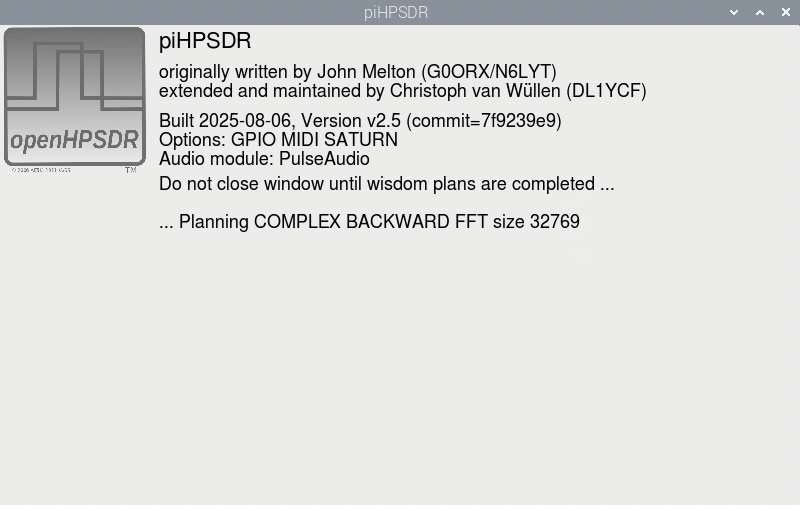
\includegraphics[scale=0.45]{Planning.png}
\caption{\pH screen while completing the \textit{wisdom plans}.}
\label{fig:Planning}
\end{figure}

If the \pH program is started for the first time, it opens a window that looks like Fig. \ref{fig:Planning}.
Besides stating a version number and the date \pH was built, the list of optional features is
documented (compile-time options,
in this case  GPIO, MIDI, SATURN) as well as the audio module used (here: ALSA) for attaching headphones
or microphones to the host computer running \pH. Information about compile-time options and the
audio modules available are given in Appendix \ref{sec:compiletime}.

What is important here that you have to wait. This only applies to the very first time you start \pH.
On CPUs with a rather simple instruction set (like the ARM processor in the Raspberry Pi, or the Apple
Silicon processor in recent Macintosh computers), this so-called  \textit{planning} step is quite fast. For
example, on my
Apple M2 Mac mini, this step only takes 6 seconds, and you have to wait for 34 seconds on a RaspberryPi 4.
On the contrary, on CPUs with
complex instruction sets, more planning is necessary: on my other Mac mini with a 3 GHz x86 processor, it
takes 16 minutes! But note
this has only to be done once, in subsequent starts of \pH, the wisdom will simply be read from
the file created during the \textit{planning}. These plans contain, for a large number of dimensions,
the fastest way to perform FFTs (\textit{fast Fourier transformations}) on the given CPU.
When this ,,wisdom'' is secured, \pH tries to detect a radio on the network. If everything went well with
the network connection, you then see a screen with a discovery menu (Fig. \ref{fig:Start}).

\clearpage
\textbf{The Start button}

\begin{figure}
\center
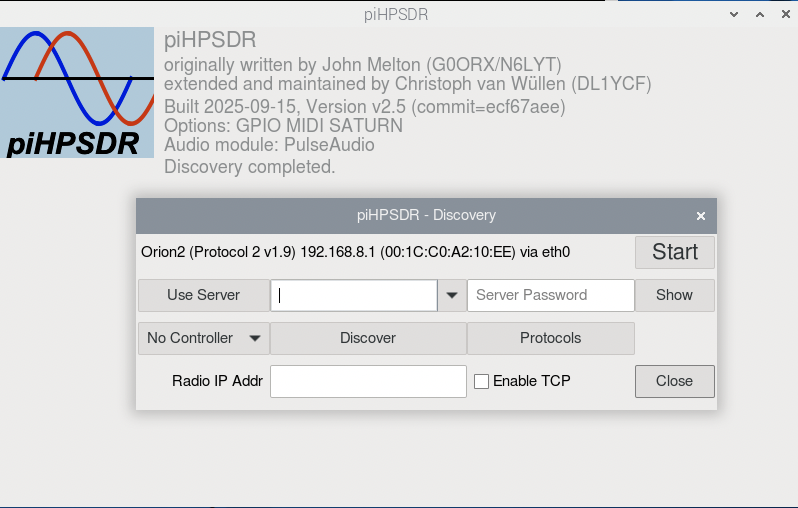
\includegraphics[scale=0.45]{Start.png}
\caption{A radio has been discovered. You are ready  to start it.}
\label{fig:Start}
\end{figure}

It is possible that the \rett{Start} button is deactivated and shows another text. \rett{In Use} at
this point means that the radio is already in use (connected by another SDR application), while
\rett{Incompatible} denotes that the radio is not compatible with this version of \pH. This
is only the case if \pH runs on the compute module inside the new Anan Saturn/G2
radios and the FPGA firmware is known to be too old (or too new)
for direct (XDMA) data transfer between the compute
module and the FPGA. Updating both \pH and the FPGA firmware to the latest version
should help in this case. Should the start button read \rett{Subnet!}, then the IP address of the
radio is outside the range of the network adapter which received the discovery packet.
In most cases when you see this, it results from a radio being caught in the act of initialising
itself, and pressing the \rett{Discover} button again to re-start the discovery process then
usually lets the problem vanish.

{\color{red} Note when using a VPN tunnel:} I have heard of cases where VPN is used to attach
a remote subnet as if it were a local one, and where the virtual  ,,ethernet adapter''
that realises the VPN tunnel is assigned a netmask that is too narrow such that the start
button is deactivated and shows the text \rett{Subnet!} although a connection is indeed possible.
In such cases, the easiest remedy is to manually type in the IP address of the radio (which is
shown in the line containing the deactivated button) in the \rett{Radio  IP Addr} text field
(see below) and then click the \rett{Discover} button.

If more than one radio is available, or a radio can be connected via more than one network interface,
you will see several \rett{Start} buttons.
If you see at least one \rett{Start} button, you can start the corresponding radio simply
by clicking that button.

The line of control elements following the radios discovered begins with the \rett{Use Server} button,
and belongs to the
client/server feature that is described in chapter \ref{sec:clientserver}, it will not be discussed
here where we now explain the purpose of the remaining control elements.
 Easiest to explain is the \rett{Close} button, this will simply terminate
the program. Most likely, you may want to go into the \rett{Protocols} menu sooner or later.
By default, \pH tries to discover the presence of a radio using all protocols known to \pH. However,
if you know that your radio, for example, uses Protocol-2, then trying to discover a Protocol-1
radio is just a waste of time. So if you know which types of radio you want to connect to, you can enable
(only) these in the \rett{Protocols} menu. The available protocols are

\begin{itemize}[font=\texttt, left=80pt]
\item[Protocol 1]{This is the "original" HPSDR protocol.}
\item[Protocol 2]{This is the "new" HPSDR protocol.}
\item[Saturn XDMA]{This is used to talk to a Saturn FPGA through the internal XDMA interface. Only available
if \pH is compiled with the \texttt{SATURN}  option.}
\item[USB OZY]{This is used to talk to a radio using the legacy USB OZY interface. Only available if \pH
is compiled with the \texttt{USBOZY} option.}
\item[SoapySDR]{This is used to talk to a radio through the SoapySDR library, for example to an AdalmPluto.
Only available if \pH is compiled with the \texttt{SOAPYSDR} option.}
\item[STEMlab]{This is used to connect to RedPitaya based SDRs through the WEB interface. Only available if
\pH is compiled with the \texttt{STEMLAB\_DISCOVERY} option. Starting the radio using this protocol is a
two-step process:
first, the RedPitaya's WEB interface is located, and the \texttt{Start} button then starts the SDR app
on the RedPitaya. Then, \pH tries to connect to this SDR app and upon success offers a new
\texttt{Start} button to start the radio. If the RedPitaya is exclusively used as a radio, it is recommended
to auto-start the SDR app
when the RedPitaya is powered up. In this case, the STEMlab protocol is not used, because the SDR app can be started through Protocol-2.}
\item[Autostart]{This is a very useful option. It indicates that if exactly one radio has been found, it is
automatically started. So in normal operation, when starting \pH subsequently, and all settings are
still valid, the radio is started without user intervention. If this option is activated and one radio is
present, you will not see this menu, so in order to make further changes here, you have to disconnect the
radio from the ethernet cable, start \pH until you see this menu, and update the \rett{Protocols}
settings. Then you can re-discover using the \rett{Discover} button.
If you have an Anan-G2 radio and activated \texttt{Autostart}, then you have a problem. Since always
exactly one radio (the G2) is discovered, you will always step over the discovery menu and start the
radio right away, which means you cannot change any setting in the discovery menu. The only way
to get of of this trap is to remove the file \texttt{protocols.props} in the directory where \pH
stores its settings. On a G2, this is usually \texttt{\$HOME/github/pihpsdr}.

}
\end{itemize}

\textbf{Connection to a radio with known IP address}

Sometime \pH \textit{needs} to know the IP address of the radio, for example to perform
a \texttt{STEMlab} discovery as described above. But also if the radio and the computer running
\pH are not on the same network segment, a successful radio discovery may only be possible
by directly querying the radio by its IP address. To use this feature,
the IP address in numerical form (xxx.xxx.xxx.xxx) can be entered in the box
with the label \rett{Radio IP Addr}. If a legal IP address is contained in this box, protocol-1 and
protocol-2 discovery queries
will  be sent to the IP address specified, in addition to the standard broadcast discovery packets which
can only reach
radios on the same network segment. With a known IP address (and if supported by the radio),  one can
connect to radios which are not on the same sub-net as the computer, in principle you can connect to any
radio on the world
provided it is on the internet. My advice is to always use this possiblitiy if the radio and the host
computer are not on the same network segment, for example if one connects to a distant radio via an
unsecured internet connection of via a VPN (VPN stands for \textit{virtual private network}) tunnel.

Note that if a radio IP address is specified, the discovery process skips sending broadcast discovery
packets if a radio could be detected on the specified IP address. So if you specify a radio IP address
and such a radio exists, \pH will not discover any other radio that might also be connected to the same
network segment. The advantage is, that the start of the radio speeds up considerably.

In rare cases (the RedPitaya STEMlab and RadioBerry cases are the only one I know of)
it is  possible to use the TCP protocol
rather than the standard UDP one for communicating with the radio. A ``TCP discovery'' will wait for three
seconds if there is no response (there will be no response unless a TCP-enabled radio is present).
Therefore, trying to connect via TCP is only done if the \rett{Enable TCP} box is checked.



The \rett{Discover} button re-starts the discovery process. This is useful if the radio has been powered up
too late and
was not yet ready when \pH was started. Simply press \rett{Discover} to start another attempt. This is
largely equivalent to quitting and restarting \pH but much more convenient.

\textbf{Specifying a ,,piHPSDR controller'' or a ,,Anan G2 panel''}


The combo-box (pop-down menu) to the left of the \rett{Discover} button lets you choose which type of GPIO
controller you
have attached to the computer.  If compiled with GPIO support (this can also be done for
programs running on a Raspberry Pi or on an internal Raspberry module of first-generation (2023) Anan G2 radios),
the menu lets you choose between

\begin{itemize}[font=\texttt, left=80pt]
\item[No Controller]{Choose this if no GPIO controller is wired to your Raspberry Pi. This is the default
when you first start \pH. Some GPIO lines are still used e.g. for PTT or CW. If this conflicts with other
hardware connected to the GPIO, it is better to compile \pH without the GPIO option.}
\item[Controller1]{Choose this if you have the original \pH controller put to the market by ApacheLabs
(or a clone thereof), called the Controller1 in the rest
of this manual.}
\item[Controller2 V1]{This option is valid for some early prototypes of the "version 2" controller with
single encoders. This special case is not covered in this manual.}
\item[Controller2 V2]{Choose this if you have a "version 2" \pH controller from ApacheLabs (with double encoders
on a single shaft), or a clone thereof.
This controller is denoted Controller2 in the rest of this manual.}
\item[G2 Front Panel]{Choose this if you have an Anan G2 radio with a built-in controller.}
\item[G2 Mk2 Panel]{Choose this if you have an Anan G2 Mk2 (also known as ,,G2 Ultra'')
radio (with LEDs in the front panel).
This tells \pH not to use any GPIO lines, if it is compiled with GPIO support. However, it is
strongly recommended \textit{not} to enable GPIO for G2 Ultras. Previously, \pH required this choice
to set up the serial line for the panel controller of the G2 Ultras, but this is now handled
automatically.}
\end{itemize}

\textbf{Attention.} Be sure to choose a controller only if such a controller is actually connected to your
Raspberry Pi. Unexpected things can happen if you chose one type of controller here but have totally different
hardware connected to the GPIO. For example, if you have a so-called ,,audio hat'' attached to the RaspPi
GPIO, then it is safest to compile \pH without GPIO support.
The same applies to G2 Ultras where GPIO lines may be used for serial connection
to the panel. Note that even if you choose \texttt{No Controller}, some GPIO lines are still used
e.g. for CW, as documented in Appendix \ref{sec:gpio}.

All settings (protocols, controller, IP address, Server address) made in this menu are stored in
radio-independent) files ( \texttt{gpio.props}, \texttt{ipaddr.props}, \texttt{protocols.props},
\texttt{remote.props})
and are restored when \pH is started the next time.

If all went well, a radio could be discovered and you hit the \rett{Start} button, the radio is started, and
if this succeeds, you see something like shown in Fig. \ref{fig:FirstDisplay}.

\begin{figure}
\center
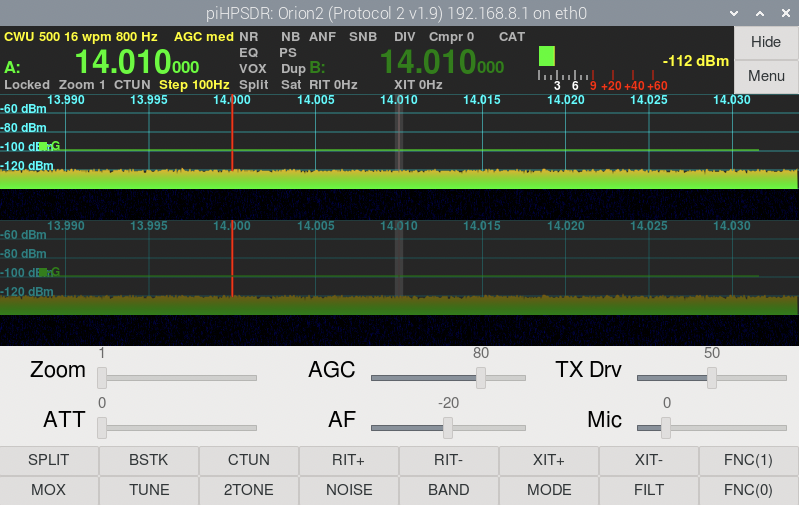
\includegraphics[scale=0.45]{FirstDisplay.png}
\caption{The radio with two RX. Sliders and Toolbar are not on display
by default when using a controller.}
\label{fig:FirstDisplay}
\end{figure}

The bottom of the window looks different (more controls) if you have chosen \rett{No Controller} in the
preceding menu.
You see two receiver panels stacked vertically, both of them having a spectrum display and a waterfall area.
At the top,
just below the window title, you have the VFO bar which contains information on the frequencies of the two
VFOs A and B,
as well as lots of further information, to be explained later. At the top right, there are two buttons
\rett{Hide}
and \rett{Menu} which will be explained in the next chapter. To the left of these two buttons, there is the
meter bar which by default is a digital S-meter. At this point, you have started \pH successfully for
the first time.

%%%%%%%%%%%%%%%%%%%%%%%%%%%%%%%%%%%%%%%%%%%%%%%%%%%%%%%%%%%%%%%%%%%%%%%%%%%%%%%%%%%%%%%%%%%%%%%%%%%%%%%%%%%%
%%%%%%%%%%%%%%%%%%%%%%%%%%%%%%%%%%%%%%%%%%%%%%%%%%%%%%%%%%%%%%%%%%%%%%%%%%%%%%%%%%%%%%%%%%%%%%%%%%%%%%%%%%%%
\chapter{Main window layout}

\section{One or two receivers}
At the end of the previous chapter (Fig. \ref{fig:FirstDisplay}),
there were two receiver panels in the
\pH window, and both including a spectrum scope
(the green-coloured noise floor) and a waterfall. The waterfall area
is completely black in the above picture since there was no RF signal.
\pH can be switched between having one or two receivers in the
\texttt{Radio} menu. If there are two receivers (called RX1 and RX2),
one of the two is the \textit{active receiver}. If you look closely
at the above picture, you will note that the spectrum scope of
the lower (RX2) panel is shaded, while it is in bright colour for RX1.
This indicates that RX1 is currently the active receiver. By simply
clicking into the panel of the other (inactive) receiver, either with
a mouse or on a touch screen, the formerly inactive receiver becomes
active.

Many conventional rigs with two independent receivers discriminate
between the \textit{main} and the \textit{sub} receiver. It is important that
this is \textbf{not} the case for \pH. In \pH, both  receivers are
largely equivalent. For example, if you start transmitting in
normal (non-split) mode, the TX frequency matches the frequency
of the active receiver, no matter whether this is RX1 or RX2.
Likewise, in split mode, the TX frequency matches the frequency
of the non-active receiver. Most of the receiver-specific controls,
for example adjusting the AF volume or the AGC gain, refer to the
current active receiver. If \pH runs with two receivers,
RX1 is always controlled by VFO-A while RX2 is controlled by VFO-B.
The VFO settings not only include the frequency but also the
current mode (e.g. LSB or CWU), the filter setting, the band and
band stack setting, whether RIT is enabled or not, and the RIT
offset. So changing the RIT value only changes it for the active
receiver. If you want  to change the RIT value for RX2 while RX1 is
the active receiver, you have to make RX2 active, change the RIT
value and then make RX1 active again.

RX1 and RX2 are largely independent. They can receive on different
bands. They can receive from different antennas provided the radio
has two RF front-end with two analog-to-digital converters (ADCs),
as most modern radios do. In this case, one usually
assigns the first ADC (ADC0) to RX1 and the second ADC (ADC1) to
RX2. This can be done in the \bltt{RX} menu.

By default, if there are two receivers, they are vertically stacked,
with RX1 in the upper part and RX2 in the lower part of the display.
This can be changed in the \bltt{Screen} menu to horizontal stacking,
where RX1 is  in the left half and RX2 in the right half of  the
display. Changing the stacking trades vertical against horizontal
resolution, of course.

\begin{figure}[ht]
\center
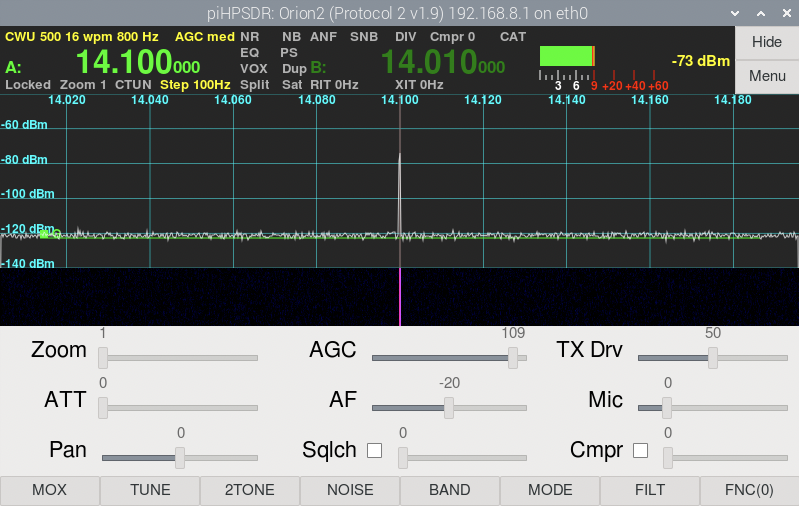
\includegraphics[scale=0.45]{SingleReceiver.png}
\caption{\pH with a single RX and all controls (Zoom/Pan,
Sliders, Toolbar) at the  bottom.}
\label{fig:SingleReceiver}
\end{figure}

Fig. \ref{fig:SingleReceiver} picture shows, for demonstration purpose, a \pH
window with a single receiver.
The RX panel only contains a
spectrum scope with a white line and no waterfall (this can be changed in the
\bltt{Display} menu). In addition, you see the toolbar
with eight buttons at the lower edge of the window, and above
it an area with sliders. Showing the sliders is the default
(and necessary) if there is no GPIO or MIDI controller attached,
since then these sliders are the only way to change, for example,
the AF volume. If there is only one receiver, it is controlled
by VFO-A. VFO-B then actually only controls controls the transmitter
if using split mode, but the data stored in VFO-B can
be quickly used, for example by copying VFO-B to VFO-A (the
\bltt{A<B} command), or by swapping the two VFOs (the \bltt{A<>B} command).

%%%%%%%%%%%%%%%%%%%%%%%%%%%%%%%%%%%%%%%%%%%%%%%%%%%%%%%%%%%%%%%%%%%%%%%%%%%%%%%%%%%%%%%%%%%%%%%%%%%%%%%%%%%%
\section{Spectrum scope options}
\label{sec:FillingGradient}

You have already seen two different spectrum scopes: in the first
picture, the  spectrum was a filled green area, while in the last
picture, there only was a white line (this is similar to what you
would see on a spectrum analyser). This can be adjusted to your
personal preference in the \bltt{Display} menu (see below). There
are two options which you can enable or disable, such that there
are four different outcomes. The first option is the ,,Filled'' option
which discriminates between a line spectrum and a spectrum which is
filled below the line. In the picture below, the first and third
example have no filling, while the second and fourth spectrum
are filled:

\begin{figure}[ht]
\center
\includegraphics[scale=0.40]{ScopeFilling.png}
\caption{Display options for the spectrum scope.}
\end{figure}

Then there is the ,,Gradient'' option. Without this option, the
spectrum is displayed in white colour. With the gradient option,
the colour changes from green over yellow towards red depending
on the signal strength (red colour is reached for S9). The above
picture demonstrates the four possible combinations, and in
the \bltt{Display} menu, you can make your choice. This setting
refers to both receivers when there are two. Note that the TX
spectrum can be a filled one or a line spectrum (to be specified
in the \bltt{TX} menu), but that there
is no gradient option.

%%%%%%%%%%%%%%%%%%%%%%%%%%%%%%%%%%%%%%%%%%%%%%%%%%%%%%%%%%%%%%%%%%%%%%%%%%%%%%%%%%%%%%%%%%%%%%%%%%%%%%%%%%%%
\section{Zoom and Pan}
\label{sec:ZoomPanArea}

\begin{figure}[ht]
\center
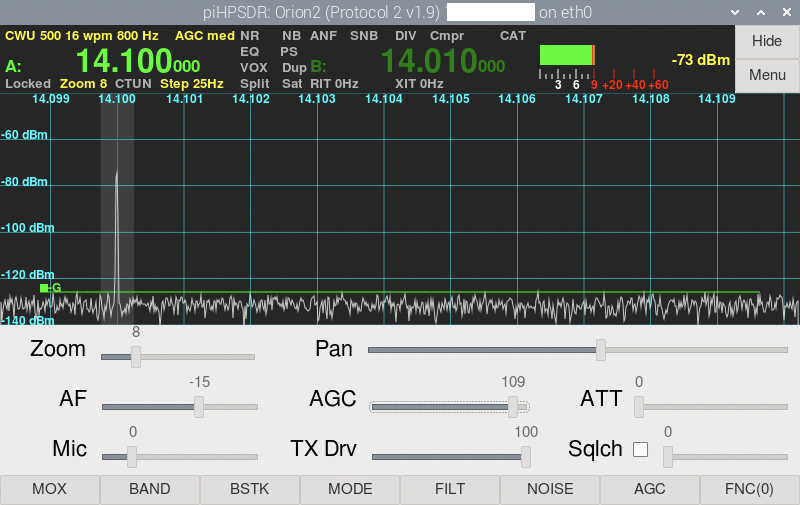
\includegraphics[scale=0.45]{ZoomPan.png}
\caption{The spectrum scope of Fig. \ref{fig:SingleReceiver} with a
large Zoom value.}
\end{figure}

The width of the RX spectrum equals the sample rate
of the receiver. This means that if you use, say,
a sample rate of 96 kHz for a receiver, its spectrum
will be 96 kHz wide, which may encompass a larger part
of the spectrum than you are interested in. As a drawback,
the part which is relevant to you may look a little bit
compressed. This is where the \bltt{Zoom} command
comes in. The zoom value can adopt integral values between
1 (no zoom) and 8. In the latter case, only 1/8 of the
overall spectrum is displayed on the screen. In the
picture below, you see that the RX scope is only 12 kHz
wide (which is 1/8 of the RX sample rate, 96 kHz in our
example). Note that what is displayed is in full resolution.
Internally, a spectrum with 8 times the number of pixels
of the screen width is created and only a part of it is
displayed. The zoom value can be changed using the \rett{Zoom}
slider (at the left edge below the RX panel).


When using a zoom value larger than one, this means that
a spectrum with more pixels than the actual screen width
is produced. One can select which part of that area
is displayed on the screen with the \rett{Pan} slider
(below the RX panel at the right side). Normally (Zoom=1),
the VFO dial frequency is exactly in the middle of the
RX scope, and marked with a thin red line. On the picture
above, the dial frequency (14.100 MHz) is found in the RX
panel close to the left edge, and this has been done
by moving the \rett{Pan} slider.

Note that the TX spectrum scope always has a fixed spectral
width, namely 24 kHz in non-duplex mode when the TX spectrum
scope is shown in the main window, and 6 kHz in duplex mode
when the TX spectrum is shown in a small separate window.

%%%%%%%%%%%%%%%%%%%%%%%%%%%%%%%%%%%%%%%%%%%%%%%%%%%%%%%%%%%%%%%%%%%%%%%%%%%%%%%%%%%%%%%%%%%%%%%%%%%%%%%%%%%%
\section{The slider area}
\label{sec:SliderArea}
Looking at Fig. \ref{fig:SingleReceiver}, one sees more sliders below the \rett{Zoom} and \rett{Pan}
sliders. Although they are largely self-explanatory, I take the occasion to describe them shortly.

The \rett{AF} slider controls the audio volume of the active receiver, from -40 to 0 dB. If moved to the
far left (at -40 dB) the audio is muted completely.

The \rett{AGC} slider controls the AGC of the currently active receiver, it goes from 0 to 120 dB. There
is a green horizontal line (with a letter G at the left edge) in the RX panadapter, and the \rett{AGC}
slider should be positioned such that the green line is at the level (or slightly above) the noise
floor. Note that the AGC value does not only depend on the attenuation/gain in the RF front end
(e. g. the position of the \rett{ATT} slider) but also on the current filter bandwidth (for a filter
10 times narrower the \rett{AGC} value can be increased by 10 dB). Note that if the green line
is higher up than the signals you want to receive, they will probably not be heard in the
RX audio.

The \rett{ATT} slider controls a programmable attenuator in the RF front end of the active receiver. For
HPSDR hardware, it goes from 0 to 31 dB. The HermesLite-II has a slider named \rett{RF} at this place,
since this radio has a programmable preamplifier/attenuator that goes from -12 to +48 dB. For the STEMlab
(RedPitaya based) radios, you find a combo-box here where you can select the fixed attenuators/preamps.
Radios which have a programmable RF gain rather than an attenuator (e.g. the HermesLite-II) have an
\rett{RF gain} slider at this position. Note that the position of these sliders is stored internally
for each band, and restored upon a band change. The idea behind this is that one usually wants no
attenuation, say, on the 10m band while it might be necessary to have some attenuation on the 80m band.

The \rett{Mic} slider adds an amplification from -12 to +50 dB to the audio signal fed to the transmitter.
This amplification is purely done numerically (no effect on any hardware) and applies to the audio signal
no matter where it comes from, let it be real microphones or virtual audio cable. For digital modes using
virtual audio cables, one normally uses no compression, no TX equaliser etc. and the \rett{Mic} slider
should stay at +0 dB. For many microphones, it might be useful to advance the \rett{Mic} slider
to positive values. For more information, see chapter \ref{sec:txchain} on the TX audio chain.

The \rett{TX Drv} slider controls the RF output power. It goes from 0 to 100 and is meant in percent. That is,
a 5-Watt radio such as the HermesLite-II should transmit 5 Watts if this slider is at position 100. See the
\bltt{PA} menu for adjusting the RF output levels.

The \rett{Squlch} slider adjusts the squelch level. If moved up from zero, the check-box will automatically
be activated. If moved down to zero, the check box will be deactivated. If you found a suitable squelch
level and want to disable squelch temporarily, you can uncheck the check box and active squelch later
on by checking it.

Note that the slider area can be hidden (removed) via the \bltt{Display} menu (see there).
%%%%%%%%%%%%%%%%%%%%%%%%%%%%%%%%%%%%%%%%%%%%%%%%%%%%%%%%%%%%%%%%%%%%%%%%%%%%%%%%%%%%%%%%%%%%%%%%%%%%%%%%%%%%
\section{The \texttt{Hide} button}
\begin{figure}[ht]
\center
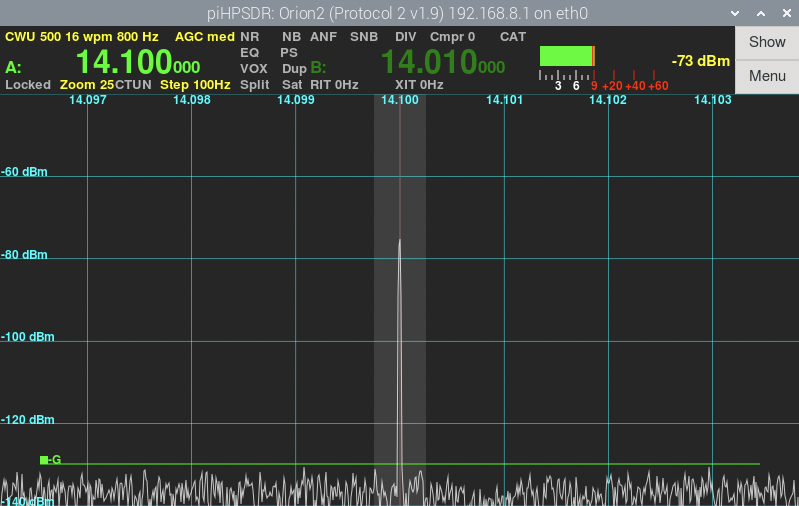
\includegraphics[scale=0.35]{Hidden.png}
\caption{\pH window with the Toolbar/Sliders/Zoom
area ,,hidden''.}
\end{figure}

On small screens, space is scarce. This in in particular true
for the vertical space if one used two RX panels and both
with a spectrum scope and a waterfall. I this case, it may be
hard to actually watch the signals if the screen is small.
This is where the \rett{Hide} button comes in. Clicking on
this button ,,hides'' the toolbar and slider area:


The text on the button then changes to \rett{Show}, and
clicking this button again will then return to the
previous display.

%%%%%%%%%%%%%%%%%%%%%%%%%%%%%%%%%%%%%%%%%%%%%%%%%%%%%%%%%%%%%%%%%%%%%%%%%%%%%%%%%%%%%%%%%%%%%%%%%%%%%%%%%%%%
\section{Window areas}

Look again at Fig. \ref{fig:SingleReceiver}! Starting from the
top, you see the title bar of the window. This bar is not visible
in full screen mode, where the size of the \pH window matches
the display size. The title bar contains some basis information
about the radio, e.g.  its type, the protocol used, the  IP
and the hardware address of the radio. If you are really interested
in this information, it is recommended to open the
\bltt{About} menu.

Between the title bar and the RX spectrum scope, you see
a small vertical area, most of  which is taken by the VFO bar
(containing the large frequency dials). At the rightmost
end of this area, you see two buttons \rett{Hide} (already
discussed) and \rett{Menu}. Clicking on the latter button opens
the main menu, which will be discussed in detail in the following
chapters. The \rett{Menu} button is really important, since it
enables access to one of the menus used for configuring \pH.
Between the VFO bar and the \rett{Hide}/\rett{Menu} buttons,
you see the meter area where you find the S-meter (during RX)
and information about output power, SWR, etc. during TX.

Below the RX  spectrum scope, you see the Zoom/Pan area with
the  Zoom and Pan sliders, as already discussed. This area
can be ,,hidden'' with the \bltt{Display} menu to save some
vertical space. Below the
Zoom/Pan sliders you see a larger  Sliders area containing
several sliders for adjusting AF volume, TX  drive level,
RX  AGC threshold, etc. Although the Sliders area can also
be hidden via the \bltt{Display} menu, you should not do so
unless you have a GPIO or MIDI controller which knobs that
you can assign to the slider functions. This is so since
for  normal operation, having access to the sliders is vital.
Remember that for temporarily enlarging the space for
the RX  panel, there is the \rett{Hide} button!

\begin{figure}
\center
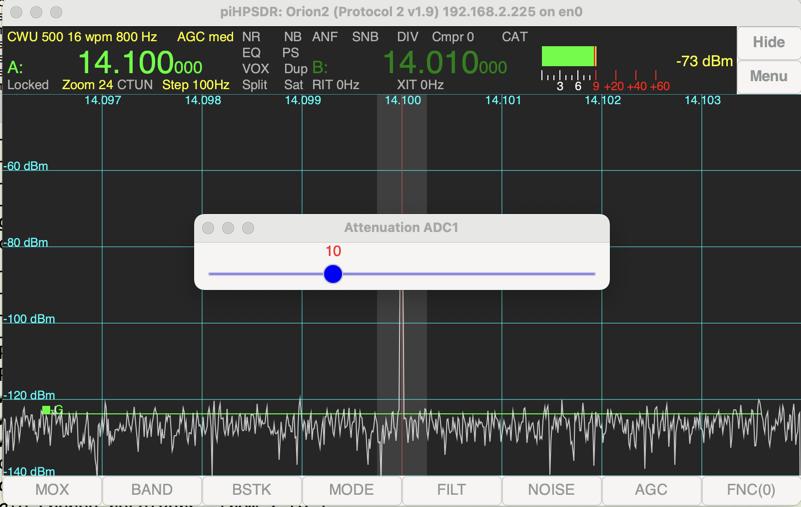
\includegraphics[scale=0.45]{SliderOnScreen.png}
\caption{A pop-up attenuation slider.}
\label{fig:SliderOnScreen}
\end{figure}

If you have a GPIO or  MIDI  console, and, say, assigned
a knob there to control the AF volume, then turning the
knob will auto-magically also move the AF slider if its
on display (that is, if the sliders area is not hidden).
If you turn a knob for which function there is slider
on display, either because the slider area is hidden or
because this function does not have a slider in that area,
then a graphical slider will temporarily pop up in the
middle of the window to inform you about the changes
you have  made. To give one example, a knob at a
MIDI console has been assigned to the RF attenuator (\bltt{Atten}
function, see Appendix A), which controls the step
attenuator in the RF front-end (if there is one). As long
as the  sliders  are  on display, the \rett{Att} slider
in the right part of the slider area moves when turning
the knob. But when the sliders are not displayed, then a slider image
pops up  on the middle of the screen, and the
bar contained therein moves when turning the knob,
and the numerical value is displayed as well (Fig. \ref{fig:SliderOnScreen}).
Such a pop-up slider always occurs if a knob on the GPIO or MIDI
console is turned and no slider associated with the value changing is
on display.

At the very bottom of the window, there is the toolbar. This can also be
individually hidden/shown via the \bltt{Display} menu. The toolbar consists
of eight ,,buttons'' which you can click with a mouse or on a touchscreen.
If you are using the original (V1) \pH GPIO controller, is has eight
push buttons below the screen and pressing those is equivalent to clicking
the buttons on the screen. You might still want to keep the toolbar on display
even if you are using the Controller1 since it shows you to which functions
the buttons are actually assigned. This assignments consists of six ,,layers''
(0 through 5). The rightmost button is hard-wired to the \bltt{Function}
command which cycles through the layers. The button text includes the
number of the currently active layer, and the button text of the other buttons
reflect the functions assigned to the buttons in the current layer.

\textbf{Bonus for mouse users only.} For the first seven toolbar buttons,
there is no difference if you do a primary or secondary mouse click on that
button (that is, it does not matter whether you use the left or right mouse
button). But for the rightmost toolbar button, a normally mouse click cycles
forward through the layers, while a secondary mouse click cycles backwards.
If you use a V2 or G2 front panel GPIO controller or a MIDI console, then you
can also map this function (\bltt{FuncRev}) to a spare button.


%%%%%%%%%%%%%%%%%%%%%%%%%%%%%%%%%%%%%%%%%%%%%%%%%%%%%%%%%%%%%%%%%%%%%%%%%%%%%%%%%%%%%%%%%%%%%%%%%%%%%%%%%%%%
\section{Mouse clicks in the main window}
The main window ,,accepts'' mouse or touchscreen click events.
Some of them come from the standard handlers of the GUI. It is
clear, for example, that clicking the \rett{Hide} or
\rett{Menu} buttons, as well as clicking one of the
toolbar buttons, will activate the function associated with
these buttons. Furthermore, the sliders (and the squelch enable/disable
checkbox) in the sliders and Zoom/Pan are are operated as usual.
But there are additional functions coded into \pH:

If there are two receivers, a mouse click (press and release) into
the panel of the non-active receiver makes it active. On the other
hand, a mouse click in the panel of the active receiver changes
the VFO frequency of that receiver to the value clicked on.
This means, if you see a signal in the spectrum scope, click
on that signal and your VFO will move (\textit{jump}) to that signal.
Note the VFO frequency will be  rounded to the next multiple of
the VFO step size when jumping by a mouse  click or
touch screen press.

The second option to change the VFO frequency of the active receiver
is to click (and hold) into its panel, then drag the mouse to the left
or to the right, and then release the button. This will shift the
VFO frequency by the amount dragged, it makes no difference
where the first click actually occurred, only the difference
in horizontal position between click and release is used. You must
drag at least three pixels so there is clear discrimination between
a \textit{VFO jump} (click then release) and a \textit{VFO drag} (click, drag,
and release) operation. Finally, the VFO frequency of the active
receiver can be changed by the scroll wheel of the mouse, if there
is any. Using the scroll wheel lets the VFO frequency move in multiples
of the VFO step size, while mouse dragging can also be used for
finer tuning.

Clicking into the VFO bar opens the \bltt{FREQ} (VFO) menu,
for the VFO-A if clicked into the left half of the bar, and for
VFO-B if clicked into the right half. This menu not only offers
the possibility for direct frequency entry, but also lets you
alter the RIT/XIT or VFO step size, or alter the Lock, Duplex,
CTUN, or Split states. So a simple click in the VFO bar
gets you quick access to often-used functions.

Clicking in the meter section (between the VFO bar and the
Hide/Menu buttons) opens the \bltt{METER} menu, where
you can change the meter properties (see below).

When operating with a mouse, there are usually two mouse buttons,
the primary button (for right-handed mouses, this is usually
the left button) and a secondary one. Secondary mouse clicks
are difficult to apply with a touch-screen. Although there are
touch-screen drivers which convert long presses to secondary clicks,
they generate, for a long press, a primary click first and a
secondary one later, so it is not possible to generate a
single ,,secondary press'' event. But for the benefit of
mouse users, secondary mouse clicks are handled in a special way:

A secondary click into the VFO bar will open the \bltt{BAND} menu,
so a band change can be made with really few mouse clicks. Likewise,
a secondary click into the panel of a receiver (no matter if it
the active or the non-active one) will open the \bltt{RX} menu
for that receiver. This can be used to change the settings of a
non-active receiver without making it temporarily active. In the
same way, a secondary click in the TX panel will open the
\bltt{TX} menu.

%%%%%%%%%%%%%%%%%%%%%%%%%%%%%%%%%%%%%%%%%%%%%%%%%%%%%%%%%%%%%%%%%%%%%%%%%%%%%%%%%%%%%%%%%%%%%%%%%%%%%%%%%%%%
\section{VFO bar and status  indicators}
\label{sec:VFObar}
\begin{figure}[ht]
\center
\includegraphics[scale=0.45]{VFObar.png}
\caption{The VFO bar}
\label{fig:VFObar}
\end{figure}

Fig. \ref{fig:VFObar} shows the VFO bar layout in more  detail.
The example shown is a VFO bar whose width is 745 pixels and
thus suitable for screens that are 1024 pixels wide (or more),
since the meter area has a fixed width of 200 pixels, and
the \rett{Hide}/\rett{Menu} buttons are 65 pixels wide. This layout is
denoted \texttt{VFO bar for 1024px windows}, as to the choice
of VFO bar layouts, see the description of the \bltt{Screen} menu.

The large dials indicating the frequencies of VFO-A and VFO-B
are easily recognised. The number to the left of the decimal
point is the MHz part of the frequency, the three  large digits
to the right  of  the decimal point is the kHz part, and
the last three (smaller) digits offer sub-kHz resolution.
You may wonder why there is  so much space to the left of
the frequencies. This is so because with the advent of
the QO-100 satellite, frequencies above 10 GHz can be
used (with the transverter bands) and therefore eleven
digits are needed!

Apart from the frequencies, you see a lot  of text, most in
light grey colour. As a general rule, a text  in grey
colour indicates a feature that is currently disabled,
while features currently active are normally shown in
yellow and sometimes in red.

At the top left  corner of the VFO bar, the mode and
filter width of the currently active receiver is displayed.
Note that this is not necessarily the width of the filter
which has been selected, if its width has been adjusted
e.g. by using controller knobs.
In Fig. \ref{fig:VFObar}, the text is \rett{USB 2.7k}
which indicates that the  mode
is USB and the filter width is about 2.7 kHz.
Note the VFO bar reports the
\textit{actual} filter width and not the name of the chosen filter,
the actual filter width can be temporarily modified for QRM fighting
if one has e.g. a console or a penal with knobs assigned to the \bltt{Filter Cut High/Low}
commands.
For the CW (CWU and CWL) modes, the CW speed (in wpm) and the side tone
frequency (in Hz) is stated as well. For CW, the filter size may be appended
by a ,,P'', which indicates whether the CW audio peak filter (see the
\bltt{Filter} menu) is effective on top of the normal filter.
For the FMN mode, an indicator of the form C=xxx.y is added if
CTCSS is enables, and then xxx.y shows the CTCSS frequency.

Now we continue line by line, from left to right and find
the string \rett{AGC med} printed in yellow. This means
that automatic gain control (AGC)  is effective  in the
active receiver, and that the AGC time constant is
intermediate. Possible values for the time constant
are Long, Slow, Medium and Fast which can be selected
in the \bltt{AGC} menu. Here one can  also disable AGC,
in this case the VFO bar shows \rett{AGC off} in grey
colour.

Continuing to the right, we see the noise reduction settings,
all printed in grey (that is, they are not effective). This
can be changed in the \bltt{Noise} menu. We have two different
noise reduction capabilities \rett{NR1} and \rett{NR2}, these
strings are printed in yellow instead of the grey \rett{NR} if
they are effective. There are also two different noise-blankers
\rett{NB1} and \rett{NB2}, the automatic notch  filter
\rett{ANF} and the spectral  noise blanker \rett{SNB}.
Besides enabling/disabling these functions, there are  further parameters
you can tweak in the \bltt{Noise} menu.

The following items indicate whether Diversity reception is enabled or disabled
(\rett{DIV}), or whether an equaliser is effective \rett{EQ}.
Since there is a separate equaliser for both RX and the TX,
the equaliser indicator, if it is effective, not only turns yellow
but reads \rett{RXEQ} while receiving and \rett{TXEQ} while
transmitting. This means, if only the TX equaliser is enabled,
the indicator will show a  grey \rett{EQ} while receiving
and a yellow \rett{TXEQ}  while  transmitting.

The last indicator in the top row  is \rett{CAT} which indicates
if the CAT module  (see the \bltt{CAT}  menu) has accepted at least
one connection. In total, \pH can be CAT-controlled simultaneously
by five different sources, two of them using a serial line and
three of them a TCP connection.

The indicators in the middle, between the VFO dials, are related to
transmitting. \rett{CMPR} indicates if a speech processor
(compressor) is enabled, if so, it prints in yellow, followed
by a number between 1 and 20 indicating the compression value in dB.
If the speech processor is used simultaneously with the continuous frequency
compressor (CFC), there is a yellow \rett{CprCfc} at this place, and if
the CFC is used but not the speech processor, the symbol is \rett{CFC on}.
\rett{Dexp} states whether the downward expander (DEXP) is active. Due to space
restrictions, this indicator is not shown for the smaller VFO bars.
\rett{PS} indicates whether adaptive pre-distortion (,,PureSignal'')
is enabled, PS settings can be made in the \bltt{PS} menu.
\rett{VOX} indicates whether VOX (voice control) is enabled. VOX means
that if  the microphone delivers an amplitude above a certain threshold,
the radio is automatically put into TX mode. Enabling/Disabling VOX
and setting the correct threshold can be done in the \bltt{VOX} menu.
Finally, \rett{DUP} indicates whether duplex mode is active.
In duplex mode, the receiver(s) continue to work during transmit. Duplex
mode when using the same antenna for RX and TX is  no fun: you not only hear
your own signal with a delay (from the cross-talk at the TRX relay), but
this cross-talk signal is  usually so strong that it leads to ,,AGC pumping'', so
your receiver is virtually deaf during the first second after TX/RX
transition. For satellite operation, on the other hand, duplex  mode
is very convenient. Here you usually have two separate and well-decoupled
antennas for RX and TX.

The bottom line of the VFO bar  indicators are related to the VFO status.
If the \rett{Locked} string is red, it indicates that the VFO is locked
and will not accept changes. There is a LOCK command which toggles the
LOCK status and which can be assigned to a toolbar button or a push-button
on a GPIO or MIDI console, but the Lock status can also be set/unset
via the \bltt{FREQ} menu, accessibly by the main menu window, or just by
clicking into the VFO bar.

The next indicator in the bottom  line indicates the Zoom factor. If the
Zoom factor is 1, the indicator is grey, otherwise it is yellow and
also indicates the factor. Then there is a string \rett{CTUN} which
indicates whether the CTUN (,,click to tune'') mode is off or on (the string
is yellow in the latter case). The step size of the VFO controlling the
active receiver is displayed next, this string is always yellow.

The split status is displayed by the next indicator, which is red in
split mode. If split mode is off, transmitting is done on the frequency
and the mode of the active receiver (if there are two receivers), or
on the frequency/mode of VFO-A (if there is only one receiver). If
split mode is on, transmitting occurs on the frequency/mode of the
non-active receiver (if there are 2) or on VFO-B (if there is only  one
receiver). Note that a frequent beginner error is to have, say,
SSB mode in VFO-A and CW mode in VFO-B. In this case, nothing is
transmitted when doing split and using the microphone. Normally one
starts with the \bltt{A>B} command (that is, copy VFO-A to VFO-B), and
then adjusts the transmit frequency.

The next indicator shows the SAT (satellite) mode, which can be off
(then the indicator reads \rett{SAT} in grey), or which can be SAT or RSAT
(then the indicator displays this string). Once SAT mode is engaged,
the two VFOs are tied together such that any frequency change of one
of the two VFOs also applies to the other VFO. This is the best way
to do cross-band operation with, e.g. the QO-100 satellite which is at
a fixed position. In RSAT mode, a frequency change of one of the VFOs
is applied to the other VFO with an opposite sign (so if you move up
VFO-A by 2 kHz, then VFO-B moves down by the same amount). This is
what one needs for low-flying satellites which have inverting
transponders which offer some sort of Doppler correction.

Finally there are the \rett{RIT} (receiver incremental tuning) and \rett{XIT}
(transmitter incremental tuning) indicators. If RIT is off,
receiving occurs on the VFO dial frequency. If RIT is on, the
indicator becomes yellow and also indicates the RIT offset, that is,
the frequency offset used while receiving. RIT is used, for example,
if during your CW QSO the frequency of the transmitter of your
QSO partner drifts and you want to follow without altering the
frequency of your own transmitted signal. The RIT indicator
corresponds to the active receiver. If XIT is active, the
indicator becomes yellow and shows the offset of the true
TX frequency from the VFO dial frequency.

Finally, in the top right corner you see a symbol with a green and a red line
which show the actual RX filter edges (in red) compared to the nominal
filter edges (in green). Both filter edges normally agree unless the actual
filter edge has been temporarily modified, e.g. to cope with QRM.
%%%%%%%%%%%%%%%%%%%%%%%%%%%%%%%%%%%%%%%%%%%%%%%%%%%%%%%%%%%%%%%%%%%%%%%%%%%%%%%%%%%%%%%%%%%%%%%%%%%%%%%%%%%%
\section{Meter section}
\label{sec:MeterSection}
Fig. \ref{fig:MeterDesigns} shows the different designs that exist for
the meter. To the left (right) there are the digital (analog) meters,
while the top panels show the meter during RX and the lower panels
during TX.

\begin{figure}[ht]
\center
\includegraphics[scale=0.45]{MeterDesigns.png}
\caption{Different designs for the meter.}
\label{fig:MeterDesigns}
\end{figure}

By default, the width of the meter section is 200 pixels, but if the current
choice of the VFO bar and the window width leaves enough space, the width
of the meter is increased to 250 pixels which allows for displaying some information
at a larger font size. For example, if the standard VFO bar for a \pH
window 800 pixels wide is chosen, and the width of the window exceeds 850
pixels, the meter automatically widens.

The design can be switched between digital and analog in the \bltt{Meter}
menu, which can be accessed quickly just by clicking into the meter area.
During RX, an S-meter is shown together with the signal level in dBm. Note
that -73 dBm corresponds to S9 for frequencies up to 30 MHz, while above
30 MHz, S9 corresponds to -93 dBm. Since the S meter is in steps of
6 dB, a signal level of S1 (below 30 MHz) corresponds to -121 dBm. In the
meter menu, one can also choose if the S-meter reading corresponds to a peak
or  an average value. Further info on the meters (e.g. switching between
,,peak'' and ,,average'' reporting)
is described in the \bltt{Meter} menu.

During TX, the output power is displayed, provided that the radio actually
reports this power. The output power meter can be calibrated (see the \bltt{PA}
menu). If the SWR exceeds a threshold for SWR warnings (the default is 1:3, but
this can be changed in the \bltt{TX} menu), the SWR indicator turns red. If,
in addition, SWR protection is enabled in the \bltt{TX} menu, the output
drive  will be reduced to zero if the SWR exceed that threshold.
Furthermore, the ALC (automatic level control) value of the transmitter is
shown. Negative ALC values (in peak mode) indicate that the volume of the TX input audio
could be increased to get full output  power. During TX (and also during RX when using
voice control (VOX), the actual level of the TX audio  signal is shown through
the small \rett{Mic Lvl} bar. The audio level is in dB from $-40\ldots0$ dB. Note that
this refers to the peak level of the  incoming ``TX microphone'' audio data, there can
be further amplification in the TX  chain through the \bltt{Mic} slider. All this
is explained in detail in chapter \ref{sec:txchain} on the TX audio chain.



%%%%%%%%%%%%%%%%%%%%%%%%%%%%%%%%%%%%%%%%%%%%%%%%%%%%%%%%%%%%%%%%%%%%%%%%%%%%%%%%%%%%%%%%%%%%%%%%%%%%%%%%%%%%
%%%%%%%%%%%%%%%%%%%%%%%%%%%%%%%%%%%%%%%%%%%%%%%%%%%%%%%%%%%%%%%%%%%%%%%%%%%%%%%%%%%%%%%%%%%%%%%%%%%%%%%%%%%%
\chapter{\pH menus: introduction}

\section{\pH menus}
Now we have a series of chapters that discuss all the \pH menus. Many menus can be
opened by a button click (or a push-button on an external controller), e.g. hitting the
\rett{MODE}, \rett{FILT}, or \rett{NOISE} button on the
toolbar you have seen in the last picture. You already know that the VFO and Meter
menus can be opened by clicking into the VFO or meter section at the top of the window.
When operating with a mouse, a secondary click in the RX or TX pan-adapter opens the
RX or TX menu.

Some remarks have to be made about menus in general. Since \pH is optimised for
working with small screens, only one menu can be open at a time. If a menu is open
and one tries to open another one, the first menu will be destroyed (closed) and the
new one will be opened. For example, if you hit the \rett{FILT} button in the toolbar
when starting from Fig. \ref{fig:MainMenu}, the main menu closes and the \bltt{Filter} menu
opens. If you try to open a menu that is already open, then the menu will be closed.
So, starting from Fig. \ref{fig:MainMenu} hitting the \rett{Menu} button again will close
the menu. Likewise, when the Filter menu has been opened, either via the Main Menu
or with the \rett{FILT} button, then hitting this button again will close the
\bltt{Filter} menu.

While the menus are looking quite diverse, some effort has been invested to keep
some things consistent throughout. For example, at the top left corner of the menu
you usually find the "Close" button which closes the menu. The close button is somewhat
emphasised (slightly larger letters, and a thin border) so you will always quickly find it.
Of course, it it possible to close a menu by deleting the menu window (on RaspberryPi,
this is the small cross at the left of the title bar) but this is neither necessary nor
recommended.

\section{Using menus \textit{and} controllers/panels}

Menus in \pH are windows that pop up if a menu is opened. These windows by default are positioned such
that they cover a relevant part of the \pH window. If you have a large display, you can move the menu
window such that it no longer covers the panadapter(s), if you want.

If a menu window pops open, its controls reflect the status of \pH when the menu opens. One can then operate
the menu, usually with a point-and-click device such as a mouse, a trackpad, or a touch screen.

If once changes the state of \pH this way, the change is immediately reflected in the menu. For example,
if you open the \bltt{Radio} menu and the split state is not active, the split checkbox in the radio
menu (see Fig. \ref{fig:RadioMenu}) is not checked. If you then click this check box, it changes to
the ''checked'' state and the Split state becomes active, as can be seen e.g. in the VFO bar. It is also
possible to change the Split state by assigning the \texttt{Split} command to a toolbar button, or to
a physical button of an external controller (GPIO, MIDI, ANDROMEDA) or a G2 built-in panel. If you do this
while the \bltt{Radio} menu is open, its Split check-box will not change although the split state changed,
as witnessed by the VFO bar.

This example demonstrates that as soon as one has opened a menu, one should use the point-and-click device
to make adjustments and then close it, before continuing operating \pH using a controller or a panel. While
\pH does not block the controller or the panel once a menu has popped open, using the panel while a menu
is open is not supported. In most cases, \pH will behave as expected, but
if you change a \pH setting with a controller or a panel while a menu is open that lets you change just
that setting, the behaviour may be unexpected or even undetermined.

\section{The main \pH menu}
\begin{figure}[ht]
\center
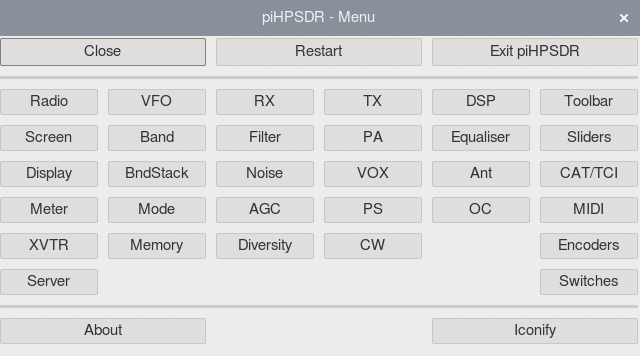
\includegraphics[scale=0.45]{MainMenu.png}
\caption{The Main men, opened by the \rett{Menu} button.}
\label{fig:MainMenu}
\end{figure}

There is one place from which \textit{all} \pH menus are at hand,
and this is the "Main Menu". It can be opened by clicking into the \rett{Menu} button at the
top right corner of the \pH window, the outcome is shown in Fig. \ref{fig:MainMenu}.
In the Main menu, there are some commands available here that do not directly affect the radio operation,
so these commands are found in the top and bottom line of the Main Menu. We first
mention the \rett{Restart} button in the middle of the top line. This restarts the
radio protocol. While not needed under normal circumstances, it my happen (especially
with beta releases of radio FPGA firmware) that the data exchange between \pH and
the radio gets out-of-sync. I observed such problems with early versions of the Protocol-2
firmware for Orion2 boards and that is the reason the \rett{Restart} button is
there, since this made a quick recovery possible without loosing the QSO.
At the bottom right, there is the \rett{Iconify} button which ,,minimises'' the
\pH window. Normally, if needed, one can do so by standard methods of the
operating system in the title bar of the \pH window. If \pH, however,
runs in full-screen mode (this is the case on very small touch screens), then the
\rett{Iconify} button to make the \pH window temporarily disappear without
breaking the connection to the radio, do some work with the operating system, and
get the \pH window back. Note in earlier versions of \pH this function was
associated with the "Hide" button in the top right corner of the main window.
Then, there are two menus (\bltt{Exit} and \bltt{About}) which are described in due course and which
one can open by clicking either \rett{Exit \pH} or \rett{About} in the main menu.

The other buttons, between the two horizontal separator lines, give access to \pH
control and fine tuning. They are organised in six columns, namely radio related
menus (first column), VFO related menus (second column), RX and TX related menus (third
and fourth column), menus affecting both RX and TX (fifth column) and, finally,
menus for adjusting how you can control \pH (sixth column), either via Toolbar,
MIDI, GPIO encoders/switches or the new G2-ultra front panel.

Not all menus appear in all cases: For example, the \bltt{Encoders} and \bltt{Switches}
menus shown in Fig. \ref{fig:MainMenu} are only present if \pH is controlled by
a GPIO-based controller. If, instead, a G2-Ultra type front panel is detected, a menu
\bltt{G2panel} appears in that place which lets you assign non-default functions to
buttons and encoders of the front panel. If there is neither a GPIO controller nor
a G2-Ultra front panel, the last column of the main menu ends with the \bltt{MIDI}
menu.

Whenever one of the sub-menus is closed, /pH writes its settings to the props file. This is not done
automatically (that is, periodically) because on some systems I/O operations affect
network traffic and may cause audio cracks. So restricting this command to situations
where ,,much happens'' anyway in the GUI seems a good compromise.
%%%%%%%%%%%%%%%%%%%%%%%%%%%%%%%%%%%%%%%%%%%%%%%%%%%%%%%%%%%%%%%%%%%%%%%%%%%%%%%%%%%%%%%%%%%%%%%%%%%%%%%%%%%%
\section{The \texttt{Exit} Menu}

\begin{figure}[ht]
\center
\includegraphics[scale=0.45]{ExitMenu.png}
\caption{The \bltt{Exit} menu.}
\end{figure}

Via the \bltt{Exit} menu, you can leave the \pH program. When leaving the program,
the radio protocol is stopped and all the settings are written to a preferences file. This
file is located in the \pH directory and takes the name XX-XX-XX-XX-XX-XX.props, where
the XX are hexadecimal numbers that encode the MAC address for the radio.
So the preferences for different radios (if you
have more than one) are stored in different files.
Note that the preferences are not only written to file when leaving the program, but also each
time a menu is opened, so the preferences file should reflect the changes you made even in the
case the \pH has crashed for whatever reason.

To leave the program, just click the
"Exit" button in this menu. If you decide you want to continue, you can leave the \bltt{Exit}
menu by clicking the "Cancel" button. This is the button which closes the menu and has
the same position and look as the "Close" buttons in all the other menus.

If \pH runs with administrator privileges, you can even leave the program and either re-boot
or switch off the computer via the "Reboot" and "Shutdown" buttons. This makes sense for setups
where a Raspberry Pi running \pH, a small SDR radio, a touch-screen and several encoders
and switches are built into a single common enclosure. On the other hand, when running
\pH on desktop or laptop computers, clicking "Reboot" or "Shutdown" both leave the \pH
program but no re-boot or shutdown takes place, due to missing administrator privileges.

%%%%%%%%%%%%%%%%%%%%%%%%%%%%%%%%%%%%%%%%%%%%%%%%%%%%%%%%%%%%%%%%%%%%%%%%%%%%%%%%%%%%%%%%%%%%%%%%%%%%%%%%%%%%
\clearpage
\section{The \texttt{About} Menu}

\begin{figure}[ht]
\center
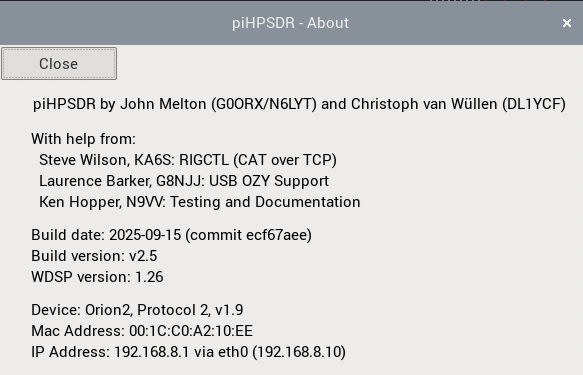
\includegraphics[scale=0.45]{AboutMenu.png}
\caption{The \bltt{About} menu.}
\end{figure}

The about menu gives you some information about \pH, first the original author,
John Melton,
and an (incomplete) list
of persons who contributed to the code, and then a statement which version of \pH
is working here, and when it has been compiled. Here you also find the version number of the WDSP
library which is the ,,engine''
running under the hood, and which does nearly all of the signal processing. If you file a bug report,
this is very important information so you should always include a screen shot of the \bltt{About}
menu when reporting problems. Of particular importance is the so-called \rett{commit},
this hexadecimal number (here: a1bbb70) identifies the exact status of the source code files
when the program has been compiled. If a string \texttt{-dirty} is appended to the version number
(here: v2.4, that is, \textit{not} dirty) this means that one or more files have been locally  modified
and do not match the commit, and problem reports from a ,,dirty'' version are difficult to handle.

Finally, there is
some data on the radio, namely the device type and version numbers, and which protocol is running.
For diagnostic purposes, you also see the MAC address of the radio, its IP address (here overwritten
with xxx.xxx.xxx.xxx)
and the
IP address of the computer running \pH (here overwritten with yyy.yyy.yyy.yyy). The IP and MAC address of
the radio are also given in the \pH main window title bar, the MAC address is of interest since the radio-specific
preferences are stored in a file whose name derived from the MAC address of the radio, replacing
the colons by dashes and appending ,,.props''.
%%%%%%%%%%%%%%%%%%%%%%%%%%%%%%%%%%%%%%%%%%%%%%%%%%%%%%%%%%%%%%%%%%%%%%%%%%%%%%%%%%%%%%%%%%%%%%%%%%%%%%%%%%%%
%%%%%%%%%%%%%%%%%%%%%%%%%%%%%%%%%%%%%%%%%%%%%%%%%%%%%%%%%%%%%%%%%%%%%%%%%%%%%%%%%%%%%%%%%%%%%%%%%%%%%%%%%%%%
\chapter[Radio-related menus]{The Main Menu: Radio-related menus}
\section{The \texttt{Radio} Menu}

\begin{figure}[ht]
\center
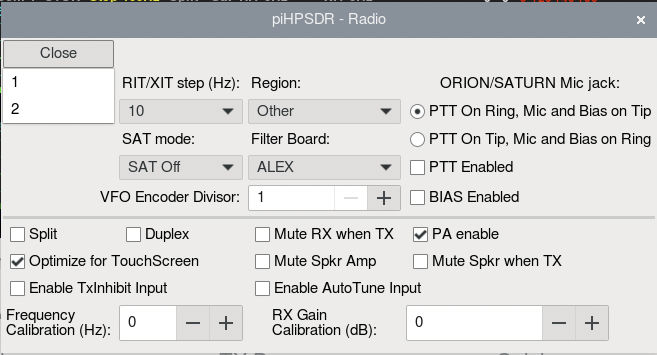
\includegraphics[scale=0.45]{RadioMenu.png}
\caption{The \bltt{Radio} menu.}
\label{fig:RadioMenu}
\end{figure}


The \bltt{Radio} menu lets you make settings which affect the general setting, and the hardware of the
radio.
The following figure (Fig. \ref{fig:RadioMenu}) shows the menu as it opens on an Anan G2 radio.
Note this menu looks slightly different for different radios and protocols, this will be discussed
at the end of the section. First, we go through all the elements we see in Fig. \ref{fig:RadioMenu},
they will be coloured red in the following list.

\rett{Receivers:} In the pop-down menu (GTK combo-box) below this string, you can select the number
of receivers that are running (well, you can choose between 1 and 2). When the number of receivers change,
the radio communication will shortly be stopped and then resumed, so do not be surprised if the spectrum
scope freezes for a second or so.

\rett{RIT/XIT step:} In the pop-down menu you can choose among three (1 Hz, 10 Hz, 100 Hz) RIT step sizes
for the VFO of the active receiver. For example, if the RIT step is 10 Hz, then you can change the RIT offset
in steps of 10 Hz with the RIT+ or RIT- buttons in the toolbar or a push-button, or with
an encoder assigned to the \bltt{RIT} command. Note that for the
\bltt{XIT+} and \bltt{XIT-} buttons, the XIT offset changes by 10 times the RIT step size. The RIT/XIT step
size is part of the RX/TX profile (see chapter \ref{sec:rxtxprofiles}) and therefore it is automatically updated
if you change the mode.

\rett{Region:} Although not obvious, this selects settings for the 60m band. Possible choices are "Other",
"UK" and "WRC15". The \texttt{Other} and \texttt{UK} choices implement the channel structure of the 60m
band according to the regulations valid in the USA and Great Britain. "WRC15" gives you a small (15 kHz
wide) 60m band according to the WRC15 (World Radio Conference 2015) document, which is now implemented in
many countries.

\rett{Orion/Saturn Mic jack:} This part of the menu is not shown for pre-Orion boards.
The Orion, Orion2, and Saturn boards can switch the connections
of the TRS microphone jack in software (hardware jumpers had to be used previously).
While the ring of the TRS plug is always connected to ground, the microphone and PTT connections are on the
ring an tip and you can choose which one is on the ring and which one on the tip. You can then separately
enable the PTT function of the jack, and select whether a bias (DC offset) is applied to the mic connection
(this is necessary for condenser (electret) microphones and detrimental if a dynamic microphone is connected without
a blocking capacitor).

\rett{Mic Input:} This is only shown for Anan G2 radios (Saturn boards).
These radios have two jacks for connecting a
microphone, either a 3.5mm TRS jack in the front panel, or an XLR connection in the back panel. The pop-down
menu lets you choose between these two options.

\rett{SAT mode:} Here you can choose between \texttt{SAT off}, \texttt{SAT}, and \texttt{RSAT}. In SAT mode,
frequency moves applied to one of the two VFOs are applied to the other VFO as well. This is convenient
for cross-band operation over satellites with (normal) linear transponders. In RSAT mode, frequency
moves applied to one of the two VFOs are applied to the other with the sign inverted, that is, if
for example you move the frequency of VFO A up by 3 kHz, the frequency of VFO B moves down by the same
amount. This is convenient for cross-band operation over satellites with inverted transponders. Inverted
transponders are sometimes find in low and fast moving satellites because this leads to some Doppler
correction.

\rett{Filter board:} Normally SDRs have some sort of built-in PA with a filter board. Filters in the TX path
between the PA and the antenna are always required, and filters in the RX path provide some protection
against ADC overloads from strong out-of-band signals. Here you can choose between \texttt{NONE},
\texttt{ALEX},
\texttt{APOLLO}, \texttt{CHARLY25}, and \texttt{N2ADR}. Choose \texttt{NONE} if none of the other cases
apply, and hope your radio does things right automatically. \texttt{ALEX} is the most frequent choice
and applies to the largest part of current HPSDR radios. \texttt{APOLLO} is an early design of a
PA/filter combination for Hermes boards, choose this if you have one. \texttt{CHARLY25} is a filter board
used in some RedPitaya based radios (STEMlab and HAMlab). If you choose this, the Attenuator slider will
disappear from the Slider area (because this design does not have a step attenuator), instead, you get
a combined Attenuator/Preamp check-box which lets you choose between zero, preamp values of 18 and 36 dB,
and attenuation values of 12, 24, and 36 dB. \texttt{N2ADR}, finally, is the filter board usually used
in combination with a HermesLite-II radio. It is controlled by the OC (open collector) bits in the HPSDR
protocol. This means if you use \texttt{N2ADR}, this will override your OC settings upon program startup.
It is possible to change the OC settings in the \bltt{OC} menu, and these settings are saved with the
preferences. Upon next program start, however, these preferences will again be overwritten as long
as the \texttt{N2ADR} filter board is chosen.

\rett{VFO Encoder Divisor:} This option applies to VFO knobs in front panels, GPIO
or MIDI controllers. In some cases, these encoders generate too many ticks per revolution,
such that it is difficult to fine tune on a signal.
If the VFO Encoder Divisor, as shown in the example, has a value of
15, only every 15$^\textrm{th}$ tick will we processed. For the default value of 1,
the divisor has no effect.

\rett{Split} Use this checkbox to enable/disable Split mode. In Split mode, the frequency of
the non-active receiver (when using two receivers) or the frequency of VFO-B (when using one
receiver) controls the TX frequency. In normal (non-Split) mode, it is the frequency of
the active receiver (2 RX) or the frequency of VFO-A (1 RX) that matters.
Note that a frequent beginner error is to have, say,
SSB mode in VFO-A and CW mode in VFO-B. In this case, nothing is
transmitted when doing split and using the microphone. Normally one
starts with the \bltt{A>B} command (that is, copy VFO-A to VFO-B), and
then adjusts the transmit frequency.

\rett{Duplex} Use this checkbox to enable/disable Duplex mode. In Duplex mode, the receiver(s)
continue working during TX. In normal setup, this is detrimental since the very strong
signal that originates from the cross-talk at the T/R relay will lead to AGC pumping,
making your receiver(s) essentially deaf for a short period after TX/RX switching.
However, when using different and well-decoupled antennas for RX and TX (this is typical
for some satellite operations), Duplex mode gives you important information, as you can
see your own down-link signal. In contrast to what is often stated, Duplex mode does not
affect the data stream between the computer and the radio, it \textit{only} determines
whether the receivers (within the WDSP library) are shut down during transmit or not.

\rett{Mute RX when TX} Normally, the receivers are shut down while transmitting, except
in duplex mode. This option (checkbox) mutes the RX audio while transmitting even if running
Duplex. It is important
to note that the RX continue to work, so you can see the signals on the RX panel, the
S-meter works, etc. This option is largely equivalent to moving the AF slider to the
minimum position while transmitting.

\rett{PA enable} This enables/disables the PA in the radio. In addition to this global
flag, there is a per-band PA enable option for the transverter bands (see the \bltt{XVTR}
menu).

Note that the last four options (\rett{Split}, \rett{Duplex}, \rett{Mute RX when TX},
and \rett{PA enable} are not shown for RX-only radios.

\rett{Optimise for TouchScreen} The normal procedure to make a selection from a
pop-down menu (such as the \rett{Receivers:} button on this screen) is to click
(and hold) it with a mouse, then drag the mouse to your choice, and then the selection
is made by releasing the mouse button. This is very difficult to achieve on a touch
screen. Therefore, if \rett{Optimise for TouchScreen} checkbox is checked, the pop-down
menus are modified as follows: You click and release on the menu button, then it pops
down and stays open. Then you make your selection by a second click/release sequence
on your choice. While this is (only a little bit) more involved than the normal procedure
when using a mouse, it is a great helper when using a touch screen. Therefore this
option is set by default, but you can uncheck it here if you prefer normal
mouse operation. Note that this option becomes effective when the next menu is opened.

\rett{Mute Spkr Amp} This box only appears on Anan-7000/8000 and G2 radios using protocol 2.
If checked, the audio amplifier driving the speakers (either the speaker jacks in the
back panel, or the built-in speakers) is disabled. This does not affect the audio signal
at the headphone jack.

\rett{Mute Spkr when TX} This box only appears on Anan-7000/8000 and G2 radios using protocol 2.
If checked, it mutes the audio amplifier driving the speakers upon transmit only.
Note that this box has no effect if TXing in CW mode or TUNE-ing such that a side tone
is not muted. It is generally \textit{not recommended} to use this option, because the
speakers emit an audible ``pop'' each time the speaker amplifier is muted or un-muted.
Some users have reported RFI problems with the speakers and this option has been added
to make it possible to mute the speakers during transmit only.

\rett{Enable TxInhibit Input} This box only appears for HPSDR (and not for SoapySDR)
radios.
For  protocol 1, TxInhibit is signalled for most radios by the Hermes IO1 bit being
cleared (the Hermes IO2 bit is used for Anan-7000/8000). For protocol 2, for most
radios the IO4 bit is used (Anan-7000/8000/G2 use the IO5 bit).
If the \rett{Enable TxInhibit Input} box is checked, ,,TX Inhibit'' will be drawn
in the top left corner of the RX1 pan-adapter if signalled. If TxInhibit is signalled
while \pH is transmitting, it will induce a TX/RX transition, and any RX/TX
transition is suppressed while TxInhibit is active. Some radios (e.g. Anan-7000) have
a RCA jack with an active-low input, and the TxInhibit bit follows that input.
Note that for effective hardware protection, processing the TxInhibit bit must
take place in the FPGA of the radio. This checkbox simply enables \pH to tell
the user about such an event.

\rett{Enable AutoTune  input} his box only appears for HPSDR (and not for SoapySDR)
radios. The AutoTune state is signalled for protocol 1 by the input bit IO3,
and for protocol 2 by the user input bit IO6 (the active state is represented
by the bit being cleared).
If \rett{Enable AutoTune  input} checked, \pH will initiate \bltt{TUNE}-ing if the
input bit becomes active, and stop \bltt{TUNE}-ing if it later on becomes inactive.
For the Anan-7000, there is no RCA jack connected with the IO3/IO6 bit, but the
input is available on the spread-out board (between the Orion-II and the PA board) and one
can easily solder a wire there to have this user input. The AutoTune input is meant to
be pulled down if e.g. a "Tune" button on an external automatic tuner is pressed.
For such a setup, it is usually recommended to use a reduced RF output level while
\bltt{TUNE}-ing  (see the \bltt{TX} menu, chapter \ref{sec:txmenu}).


\rett{Frequency Calibration} Here you can set a frequency offset (in Hz). This offset
will be added to all frequencies sent to the radio. This means that if you discover that
a reference signal occurs in your RX panel at 10001 kHz where it should occur at 10000
kHz, you have to set the calibration value to -1000. Note it is an absolute value,
which will we applied to all frequencies.

\rett{RX Gain Calibration} Here you can calibrate your RF front end. To this end, you
need a highly accurate signal source of, say, -73 dBm. Connect this source to your
radio and tune on the signal. If the signal reported by the meter
appears too strong (say, at -65 dBm),
\textit{decrease} the
calibration value with the spin button until the meter shows the correct level.
The RX gain calibration value can be viewed as the  amplification/attenuation of
a virtual device you
would need in your RF front end. Therefore, you need a negative calibration value (attenuation)
if the signal in the meter is too strong. For most HPSDR radios, the default value is
zero. For the HermesLite-II and other radios using the AD9866 chip, the default
value is 14, but this may depend on the RF front end.

There are some further check boxes in the \bltt{Radio} menu that you cannot see
in Fig. \ref{fig:RadioMenu}, since they only appear for specific radio hardware.
They appear to the right of the touch screen optimisation check box
and will be listed here.

\rett{HL2 audio codec} This box only appears if the radio is a HermesLite-II (HL2). Some
of these radios are equipped with an audio codec and a modified firmware. The
audio codec must be enabled by setting a specific bit in the HL2 protocol,
and this check box enables/disables this bit. Furthermore, if this check box
is enabled, RX audio data is sent to the HL2.

\rett{HL2 CL1/2} This box only appears if the radio is a HermesLite-II (HL2). This
radio has two SMA jacks denoted CL1 and CL2. If this box is checked, CL1 can be
used as a master clock input for a 10 MHz clock, while CL2 then is a master
clock output (also 10 MHz).

\rett{Anan-10E/100B} This box only appears for Hermes boards. While the Anan-10E and
the Anan-100B identify themselves as Hermes boards, they have a FPGA with limited
resources and this affects the allocation of PureSignal feedback channels. To make
PureSignal work on these machines, you have to check this box in the \bltt{Radio} menu.

\rett{Swap IQ} This box only appears for radios connected via the SoapySDR library. If checked
the I and Q samples are exchanged, both in the receivers and in the transmitter. An indication
that this is necessary is if you see signals with a frequency above your dial frequency in
the left half of the RX panel, or if you have to go to LSB to receive USB signals. If you
observe this behaviour, check this box.

\rett{Hardware AGC} This box only appears for radios connected via the SoapySDR library.
If checked, automatic gain control (AGC) that is implemented in hardware in the radio is enabled.

\textbf{ATLAS bus options.} For legacy ATLAS bus radios, a number of additional settings have to be
made. Therefore, the area where we have seen the Orion microphone options now contains ATLAS bus
settings, as shown in Fig. \ref{fig:RadioMenuMetis}. You will see this only if the radio identifies
itself as a METIS board.

\begin{figure}[ht]
\center
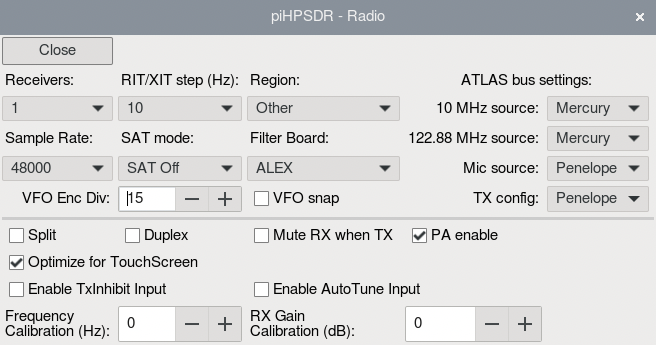
\includegraphics[scale=0.45]{RadioMenuMetis.png}
\caption{The \bltt{Radio} menu for a legacy METIS board.}
\label{fig:RadioMenuMetis}
\end{figure}

The first difference you notice is that at the left edge of the menu, in the middle,
there is a new \rett{Sample Rate:} pop-down menu. This has nothing to do with the
ATLAS bus, this occurs if the radio is connected via Protocol-1, as it is often the case for
legacy radios. In Protocol-1, all receivers share the sample rate, therefore it is set in the
\bltt{Radio} menu. The same applies for SoapySDR radios. In Protocol-2 on the other hand, each
of the two receivers can have its own sample rate, therefore the sample rate is specified
in the \bltt{RX} menu. The ATLAS bus settings are at the right edge of the menu (see Fig.
\ref{fig:RadioMenuMetis}. The ATLAS bus has separate receiver and transmitter plug-in boards.
To build a radio, they must be synchronised somehow, and therefore their clocks cannot run
independently, but there must be a master clock.

\rett{10 MHz source:} This selects the 10 MHz master clock, which can be either \texttt{ATLAS}
(the bus itself is the source), \texttt{Penelope} (the transmitter board is the source),
or \texttt{Mercury} (the receiver board is the source).

\rett{122.88 MHz source:} This selects the 122.88 MHz master clock, which can be either
\texttt{Penelope} or \texttt{Mercury}.

\rett{Mic source:} This selects where the microphone samples that are sent to the computer
originate, that is, where your microphone has to be connected. The default is
\texttt{Penelope}, this means the microphone is connected to the transmitter board. The
other choice is \texttt{Janus}. The \texttt{Janus} board is simply an ADC/DAC board (not
a radio) and used in some very early setups.

\rett{TX config:} This indicates which transmitter board is present on the bus. It can
be \texttt{No TX}, if this is a receive-only radio, \texttt{Penelope} or \texttt{Pennylane}.
The \texttt{Pennylane} is a later version of the Penelope transmitter board, the essential
difference is that it can control the output signal level. In the Penelope case,
\pH will scale the IQ samples to provide TX drive control.

\rett{Janus Only} This box is for ATLAS systems that only have a Janus ADC/DAC card,
and will only appear for OZY (USB-connected) boards. While this hardware is not a radio,
external hardware such as the SDR-1000 can be connected to the Janus card. If this
option is checked, \pH assumes that the radio is controlled outside \pH, and
will thus only process the data stream but not try to send any commands to the radio.

Note that I have no access to such legacy radios, so the \pH code to handle these radios
is partly built on speculation (that is, studying the specs) and exchanging e-mails with
people who still run such hardware. If you meet any inconsistencies, please contact
the author.

%%%%%%%%%%%%%%%%%%%%%%%%%%%%%%%%%%%%%%%%%%%%%%%%%%%%%%%%%%%%%%%%%%%%%%%%%%%%%%%%%%%%%%%%%%%%%%%%%%%%%%%%%%%%
\section{The \texttt{Screen} Menu}

The \bltt{Screen} menu lets you dynamically change the font used by \pH and
the size of the \pH main
window, it also lets you choose between different VFO bar layouts that are designed to fit
on a screen with a given width. Furthermore, one
can select whether the Zoom/Pan, the Sliders, or the Toolbar area are shown or hidden.
 The menu is opened
via the main menu and the \bltt{Screen} button and is shown in Fig. \ref{fig:ScreenMenu}.

\begin{figure}[ht]
\center
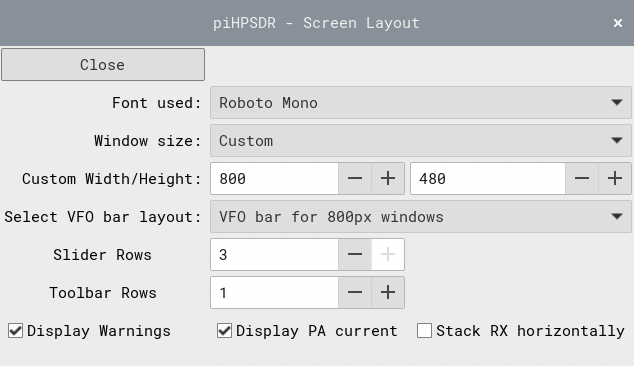
\includegraphics[scale=0.35]{ScreenMenu.png}
\caption{The \bltt{Screen} menu.}
\label{fig:ScreenMenu}
\end{figure}

In the first line, starting with \rett{Font used:},
 there is a combo-box for choosing the font. Currently, the choices
are \rett{FreeSans}, \rett{Roboto Mono}, \rett{Open Sans} and \rett{Piboto}. Changing
the font affects all menus, the slider, zoom and tool bars, as well as the VFO bar.
The default font is \rett{FreeSans} simply because it is supposed to be available on all
systems. The \rett{Open Sans} and \rett{Piboto} fonts are often told to have a
better on-screen legibility. Some people prefer mono-spaced fonts, therefore \rett{Roboto Mono}
is included in the list.

It is possible that the VFO bar layout does not look OK if you choose a font
that is not installed on your system because the system then falls back to some
default that is hard to predict. The list of fonts currently installed can be
obtained with the \texttt{fc-list} command, but
if one or more of these fonts are not available on your system, this can easily be
cured: all fonts offered in the menu can be downloaded
free of charge from the internet, installation on LINUX usually requires to create
a directory \texttt{\$HOME/.fonts} (if it not exists already), then copy the downloaded
font files (\texttt{*.otf} or \texttt{*.ttf}) to that directory and run the command
\texttt{fc-cache -v -f} in a terminal window. Installation on MacOS is even simpler:
double-clicking a font  (\texttt{*.ttf}) file will open the MacOS FontBook application
which shows you the new font, and then click on the "Install" button.

In the second line, starting with \rett{Window size:}, one can choose the size of the \pH window.
Currently the choices are \rett{Full Screen}, \rett{Custom}, \rett{640*400}, \rett{800*480},
\rett{1024*600}, and \rett{1280*720}. For the \rett{Full Screen}  choice, the \pH will occupy the entire
screen space (in a multi-monitor setup, this is the area of the monitor
on which the \pH window was opened upon program start).
For \rett{Custom}, \pH uses the screen dimensions specified by the spin buttons
in the third line. Note these buttons are only active if a custom layout is chosen. The other choices
set the screen dimensions as indicated. One can, for example, set and use a preferred custom size,
and temporarily switch to a small pre-defined geometry if one
needs screen space for other work. Switching back to \rett{Custom} then restores the preferred
window size.

\begin{figure}[ht!]
\center
\includegraphics[scale=0.30]{VFObarChoice.png}
\caption{Five choices for the VFO bar built into \pH.}
\label{fig:VFObarChoice}
\end{figure}

If the window width is decreased such that the VFO bar currently chosen does no longer fit,
\pH automatically switches to a smaller VFO bar, the
current choice shown in the
pop-down menu \rett{Select VFO bar layout} is updated. This menu lets you choose
the layout of the VFO
bar. In Fig. \ref{fig:VFObarChoice} five pre-defined layouts are shown.

These layouts require a screen size of 1152, 1024, 896, 800, and 640 pixels (from top to
bottom). Screens slightly wider (about 50 pixel) than these minimal values then allow for a larger meter
area with increased readability, this enlarged meter is automatically used if the display
width permits. There is one even larger VFO bar (for a screen width of 1960 pixels) available
that is not shown but does not look different from the topmost one in Fig. \ref{fig:VFObarChoice}.
The VFO bar has been described in detail in chapter
\ref{sec:VFObar}. If you choose a VFO bar layout that is wider than the current
window width allows, the window width is automatically adjusted (increased) when using a custom
dimension, and one advances to a larger pre-defined size if using a non-custom size. On the
other hand, choosing a VFO bar layout that is smaller than before does not affect
the screen dimensions, but there will then be some empty space between the VFO-B
frequency and the meter. Note that the smallest VFO bars do not offer enough space to display all controls:
for example, the indicator for the downward expander and the actual filter edges are  missing
in  the smallest layouts, but if one is restricted to such small screen one has to live with it.

\begin{figure}[ht!]
\center
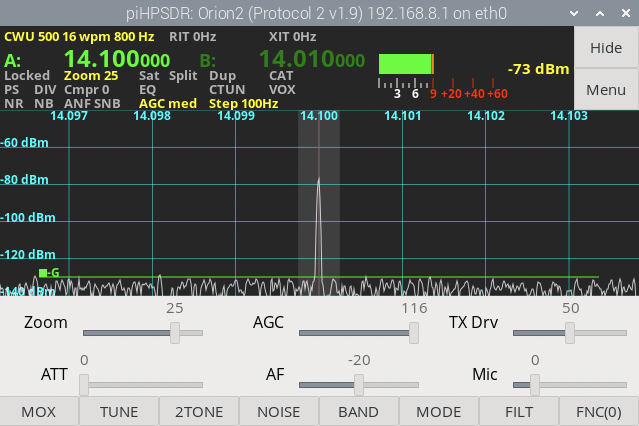
\includegraphics[scale=0.45]{640x400.png}
\caption{\pH running in a 640 x 400 window.}
\label{fig:640x400}
\end{figure}

Fig. \ref{fig:640x400} shows, as an example, \pH running in a window as small
as 640*400 pixels. It is admitted that this looks rather squeezed, and this
will probably look over-crowded when running two receivers. However, for
portable operations such small windows are often desired,
if \pH is to be run alongside with a logbook and digi mode program on a laptop.
Note that the \pH menus are designed to fit on a window 800*480 pixels large and might
not fit into a \pH window smaller than that.

\rett{Stack receivers horizontally}. If checked, this puts the panels
of the two receivers (if two receivers are used) side-by-side instead of on top
of each other.

\rett{Display Zoom/Pan} This option can be used to show/hide the Zoom and
Pan slider below the RX or TX panel. If you do not use Zoom, or control
Zoom via an external GPIO or MIDI controller, this can be used to save
some vertical space.

\rett{Display Sliders} This option can be used to show/hide the slider area
(that is where the AF gain and the Drive slider resides).
Hiding them makes little sense unless you
have a GPIO or MIDI controller. For temporarily gaining vertical space,
use the \rett{Hide} button at the top right of the main window.

\rett{Display Toolbar} This option can be used to show/hide the toolbar. This
only makes sense of using an external GPIO or MIDI controller. Note that
when using the \pH Controller1, the toolbar should remain on display since
this then serves as an indication which function is associated with each of
the 8 push buttons immediately below the screen.

\rett{Display Warnings} There are several non-fatal conditions that can
be displayed either on the pan-adapter of the first receiver or, in non-duplex
mode, on the TX pan-adapter. Normally these warnings are no reason to worry
if you see them  only occasionally. These conditions are

\textbf{Sequence Error}. Packets from the radio arrive in the wrong order, or packets
are missing. If this occurs frequently, check the connection between the radio and
the host computer.

\textbf{ADC overload}. The RF input level is too high for one of the analog-to-digital
converters. If you see this, increase attenuation in the RF front end.

\textbf{TX FIFO under run/over run} The TX IQ data packets sent to the radio while transmitting
either arrive too fast or too slow, such that the first-in/first-out queue of TX samples
inside the FPGA of the radio either overflows or drains.

\textbf{High SWR} During TX, an SWR above the SWR threshold has been detected. If this occurs
frequently, check your antenna. The SWR warning threshold (default: 3.0) can be set in the
\bltt{TX} menu. Because the forward and reflected power used to calculate the SWR have
possibly been measured at slightly different points in time, the calculated SWR may be
much too high at the beginning or the end of an RF pulse. \pH has been instrumented to
avoid such false warnings by using power readings averaged over some time, but it still
cannot be excluded that a too high SWR is reported for a short amount of time.

\rett{Display PA current} If this is checked, the PA supply voltage and the PA current
are shown while transmitting. Such data is only available for Orion-II and SATURN boards
(Anan-7000/8000 and Anan-G2) and the HermesLite-II.
For the HermesLite-II, the PA temperature and the PA current are shown.
%%%%%%%%%%%%%%%%%%%%%%%%%%%%%%%%%%%%%%%%%%%%%%%%%%%%%%%%%%%%%%%%%%%%%%%%%%%%%%%%%%%%%%%%%%%%%%%%%%%%%%%%%%%%
\section{The \texttt{Display} Menu}

The \bltt{Display} menu is used to customise the overall layout of the \pH
window and the pan-adapters of the active receiver. Adjustments
for the TX pan-adapter must be done in the \bltt{TX} menu. The menu has two sub-menus,
namely the general settings and the peak label settings, the selection is done
in the topmost row.

\subsection{Display Menu: General}

For the general settings, the \bltt{Display} menus shown
in Fig. \ref{fig:DisplayMenuGeneral}.

\begin{figure}[ht]
\center
\includegraphics[scale=0.45]{DisplayMenuGeneral.png}
\caption{The \bltt{Display} menu (General settings).}
\label{fig:DisplayMenuGeneral}
\end{figure}



\rett{Frames Per Second:} This adjust how often the RX display is re-drawn.
10 frames per second (the default) is a good value.

\rett{Panadapter High:} This value is the dBm value of the RX signal strength at the
top of the RX spectrum scope. A value of -40 dBm corresponds to S9 + 33 dB for HF
signals.

\rett{Panadapter Low:} This value is the dBm value of the RX signal strength at the
bottom of the RX spectrum scope. A value of -140 dBm is usually low enough such that
the noise floor is still on display.

\rett{Panadapter Step:} This value is the spacing of the horizontal lines on
the spectrum scope. Lines are drawn at dBm values that are multiples of the step
size.

\rett{Waterfall High:} This is the RX dBm value that will lead to the brightest
colour (yellow) in the waterfall. If the \rett{Waterfall Automatic:} box is checked
(see below), this spin button is greyed out and inactive.

\rett{Waterfall Low:} This is the RX dBm value below which the waterfall will be black.
If the \rett{Waterfall Automatic:} box is checked
(see below), this spin button is greyed out and inactive.

\rett{Waterfall Automatic:} If this box is checked, the \rett{Waterfall High} and
\rett{Waterfall Low} parameters are not used. Instead,
the lowest and highest signal strength in the RX spectrum are automatically determined
in each update of the waterfall, and these min/max values
are then used instead of the waterfall High/Low control values to determine which
colour belongs to which signal strength.

\rett{Detector:} Here one can choose between Peak, Rosenfell, Average and Sample. The
Rosenfell detector is probably closest to what one knows from a spectrum analyser.
The Average detector is usually preferred since it is less ,,nervous''.

\rett{Averaging:} Here the possible choices are None, Recursive, Time Window and
Log Recursive. For the details, see the WDSP manual.

\rett{Av. Time (ms):} If averaging is used for the spectrum scope, the time
constant involved in averaging can be set here.

\rett{Fill Panadapter} This is used to enable/disable the ,,Filling'' option
for the RX  spectrum scope (see chapter \ref{sec:FillingGradient}).

\rett{Gradient} This is used to enable/disable the ,,Gradient'' option
(colour coding) for the RX spectrum scope (see chapter \ref{sec:FillingGradient}).

\rett{Display Panadapter}. This option enables/disables the pan-adapter display
on the RX panels. With the pan-adapter enabled, you can have the waterfall alone.

\rett{Display Waterfall} This option enables/disables the waterfall display
of the RX panels. Note if both the waterfall and the pan-adapter is disabled,
there will simply be a large ,,hole'' in the \pH window. This makes little sense
except on machines with very weak CPUs, since \textit{not} displaying neither waterfall
nor pan-adapter saves some CPU time in the graphics back-end.

\rett{Waterfall Height (\%):} This parameter can be chosen between 20 and 80
(percent) with the spin button to the right of this label,
and only has an effect if \textit{both} the panadapter and the waterfall are displayed.
In this case, the parameter determines how much vertical space
the waterfall gets, as a percentage of the total height of the panel for the
receiver. The default value is 50 and means that panadapter and waterfall
are of equal height.

\subsection{Display Menu: Peak Labels}

The ``Peak Labels'' sub-menu allows one to control if and how labels
(values in dBm) are printed at the most prominent peaks on the
RX panadapter (Fig. \ref{fig:DisplayMenuPeak}):


\begin{figure}[ht]
\center
\includegraphics[scale=0.45]{DisplayMenuPeak.png}
\caption{The \bltt{Display} menu (Peak label settings).}
\label{fig:DisplayMenuPeak}
\end{figure}

\rett{Label Strongest Peaks} This enables peak detection and labelling.

\rett{Label in Passband Only} If the box is checked only the peaks within the
current filter pass-band  are shown.

\rett{No Labels Below Noise Floor} This suppresses labelling of peaks below the noise floor.

\rett{Number of Peaks to Label:} Set maximum number of peaks to be shown. There can always be less,
but no more than this number. The strongest peaks will be labelled first.

\rett{Ignore Adjacent Peaks:} Determine how close two peaks can be such that both are labelled.
The higher the number the closer the peaks can be to each other. It's a divisor of the
full window width so setting it to 1 will mean only one peak can occupy the entire window,

\rett{Noise Floor Percentile:} This is the percentile setting that defines the noise floor. If the
percentile is 50, then the noise floor is the level of that pixel that is in the middle of the list
if all pixels are sorted by their dBm value (a safety margin of 3 dBm is added).
If the \rett{No Labels Below Noise Floor} box is ticked
peaks below this value will not be labelled.


%%%%%%%%%%%%%%%%%%%%%%%%%%%%%%%%%%%%%%%%%%%%%%%%%%%%%%%%%%%%%%%%%%%%%%%%%%%%%%%%%%%%%%%%%%%%%%%%%%%%%%%%%%%%
\section{The \texttt{Meter} menu}

\begin{figure}[ht]
\center
\includegraphics[scale=0.45]{MeterMenu.png}
\caption{The \bltt{Meter} menu.}
\label{fig:Meter}
\end{figure}

The \bltt{Meter} can either be opened simply by clicking in the meter
area, or through the main menu. Only few choices can be made here.

\rett{Meter Type:} Here you can select between a digital and an analog
meter. The four different designs (either analog or digital, and during
RX or TX) have already been shown in Sec. \ref{sec:MeterSection}.

In both cases, there is a choice between Peak and Average reading, which
refers to peak envelope power and average power. Here averaging is done
over relatively short times. For a two-tone signal for example, the peak
reading is 3 dB above the average reading.

\rett{S-Meter Reading:} Here you can choose whether the S-meter reports
a Peak or an Average value (default is Average).
Note, however, that in order to make the
display less ,,nervous'' a moving average with a rather long time constant
(about 0.5 sec) has been implemented on top of both the Peak and Average
S-meter readings.


\rett{TX ALC reading:} Here, the possible values are again Peak and Average.
 Normally one uses the peak ALC value. If it is negative, the level
of the TX audio signal or the Mic gain slider should be increased.
This is very important since, for example,
PureSignal only works if the TX audio input has maximum amplitude,
so you can put the drive slider to zero, then put the radio into TX mode,
speak into the microphone and slowly increase the Mic gain until the
ALC value shown is about zero (if the ALC value is positive, you
have to reduce the Mic gain). The average TX ALC
value only is of interest if  you search for settings for the speech processor
or the continuous frequency compressor. For normal speaking into the microphone,
the average ALC value will be negative even if the Mic gain slider is adjusted
for zero peak ALC value. A compressor will distort the TX audio such that this
gap gets smaller. More details can be found in chapter \ref{sec:txchain}
discussing the entire TX audio chain.

For RX-only radios, the TX ALC setting will not be shown in the menu.

%%%%%%%%%%%%%%%%%%%%%%%%%%%%%%%%%%%%%%%%%%%%%%%%%%%%%%%%%%%%%%%%%%%%%%%%%%%%%%%%%%%%%%%%%%%%%%%%%%%%%%%%%%%%
\section{The \texttt{XVTR} (Transverter) Menu}

\begin{figure}[ht]
\center
\includegraphics[scale=0.45]{XVTRMenu.png}
\caption{The \bltt{XVTR} (transverter) menu.}
\label{fig:XVTRMenu}
\end{figure}

The \bltt{XVTR} menu lets you define up to ten additional bands
that you can work on using transverters. The bands
should normally be beyond the standard frequency range of
the radio, otherwise the calculation of a band from
a given frequency will sometimes not work.
Fig. \ref{fig:XVTRMenu} shows the \bltt{XVTR} menu with data
for an example for a transverter which you can drive with frequencies
between 28 and 30 MHz and which will convert them to the frequency
range 144 to 146 MHz, and which will receive frequencies in that
range and mix them down to the 10m band. The data you have to enter
in the \bltt{XVTR} menu (use the first free entry) are as follows:

\rett{Title} In this column, enter a name for your band. You can choose
whatever name you want, this is the one that will be displayed in the
\bltt{Band} menu. In the present example, use "144" or "144 MHz" or "2m".
If the title string is empty, all transverter data for this band will
be cleared.

\rett{Min Frq} Enter the lowest frequency of the transverter band in MHz,
in the present case, 144.

\rett{Max Frq} Enter the highest frequency of the transverter band in MHz,
in the present case, 146.

\rett{LO Frq} This is the frequency offset (in MHz) between the radio frequency and
the operating frequency. In this case, use 116. From this offset, radio frequencies
between 28 and 30 MHz will be used for operating frequencies between 144 and 146 MHz.

\rett{LO Err} This entry can be used for a fine calibration of the frequency. The value
(in Hz) is added to the local oscillator (LO) frequency in MHz.

\rett{Gain} For each transverter band, the RX gain of the transverter can be specified here.
If the transverter has a positive gain, the signal will appear too strong in the
meter and the pan-adapter, so
entering a positive number here will \textit{reduce} the dBm reading in the meter area.
This setting affects the meter reading, and the RX pan-adapter and waterfall.

\rett{Disable PA} This checkbox is only present for HPSDR (Protocol-1 and Protocol-2) radios and
indicates that the PA of the radio should be disabled
when using the transverter band. This implies that the radio has some sort of
low-power output that is used to drive the transverter.

\rett{Update} When entering data in the text fields, it does not become effective
immediately. The data is stored if you leave the menu, but also if you push the
\rett{Update} button. After pressing this button, the text fields will be re-generated,
so if you have typed in, for example, "144" as the minimum frequency, this text field
will change to "144.000". Consistency checks are performed as well: the minimum and maximum
frequencies are recalculated from the local oscillator frequency and the frequency range
of the radio, if something does not fit. It is therefore recommended to push
\rett{Update} and review the text fields before leaving the \bltt{XVTR} menu.

\begin{figure}[h!]
\center
\includegraphics[scale=0.45]{QO100-XVTR.png}
\caption{\bltt{XVTR} setup for QO-100 operation.}
\label{fig:QO100-XVTR}
\end{figure}

To give an example of how to setup transverter operation, a sample setup for QO-100 operation
with an AdalmPluto is given.
The Pluto is
operated via the SoapySDR interface. For receiving in the 10 GHz band, one uses a so-called
LNB (low noise block) in the focus of the parabolic antenna which converts the 10 GHz signal down
to about 740 MHz. The setup for defining the "QO100" transverter band is shown in Fig.
\ref{fig:QO100-XVTR}. Since the Adalm Pluto is operated via the SoapySDR interface, there are no check boxes
for disabling the PA.

\begin{figure}[ht]
\center
\includegraphics[scale=0.45]{QO100-BandMenu.png}
\caption{The \bltt{Band} menu after defining the QO100 band.}
\label{fig:QO100-BandMenu}
\end{figure}

The LO (local oscillator) frequency is always chosen such that it is below the RX frequency,
and the difference between the RX frequency and the LO frequency is the frequency the radio
is operating on. The name (here: QO100) can be chosen as one likes, but it cannot be left
empty. Once the transverter band has been defined, it shows up in the \bltt{BAND} menu
(see Chapter \ref{sec:bandmenu}), as shown in Fig. \ref{fig:QO100-BandMenu}. Note this is
a screen shot from operation with an Adalm PLUTO, where the 70 MHz (4 m) band is the lowest one.

\begin{figure}[ht]
\center
\includegraphics[scale=0.45]{QO100-Waterfall.png}
\caption{Working QO100 with \pH and the Pluto.}
\label{fig:QO100-Waterfall}
\end{figure}



To make QO-100 Operation easy, the working frequencies, the CTUN mode etc. should be
stored in the first band stack entry of the QO100 and the 13 cm band. To this end,
click on the QO100 in the band menu (Fig. \ref{fig:QO100-BandMenu} and adjust the VFO-A
frequency until the display reads 10489.500 MHz. Now swap VFO-A and VFO-B (\bltt{A<>B} command)
and enter 2400 MHz into VFO-A using the \bltt{VFO} menu (Chapter \ref{sec:vfomenu}). and
swap the VFOs again. SAT mode will now ensure the 10.489 GHz Receive
Frequencies and the 2.4GHz Transmit frequencies track correctly when changes are made
to the Receive frequency. \pH will now remember these settings when you select
the bands. The complicated swapping was necessary since band stack entries will
only be stored from VFO-A.


Fig. \ref{fig:QO100-Waterfall} (a contribution from a ham using the Adalm Pluto for QO-100
operation) gives an impression of how this actually works.
Note that the
default setup
is working Split, Duplex and SAT. Split mode implies that VFO-B is used for transmitting.
Duplex mode implies that the receiver continues to work while transmitting so you can watch
and hear your own signal.
The TX spectrum scope then appears during transmitting in a small separate window.

%%%%%%%%%%%%%%%%%%%%%%%%%%%%%%%%%%%%%%%%%%%%%%%%%%%%%%%%%%%%%%%%%%%%%%%%%%%%%%%%%%%%%%%%%%%%%%%%%%%%%%%%%%%%
\section{The \texttt{Server} Menu}
This menu is part of client/server remote operation, which is explained in chapter \ref{sec:clientserver}.
%%%%%%%%%%%%%%%%%%%%%%%%%%%%%%%%%%%%%%%%%%%%%%%%%%%%%%%%%%%%%%%%%%%%%%%%%%%%%%%%%%%%%%%%%%%%%%%%%%%%%%%%%%%%
%%%%%%%%%%%%%%%%%%%%%%%%%%%%%%%%%%%%%%%%%%%%%%%%%%%%%%%%%%%%%%%%%%%%%%%%%%%%%%%%%%%%%%%%%%%%%%%%%%%%%%%%%%%%
\chapter[VFO-related menus]{The Main Menu: VFO-related menus}

In this chapter we discuss the menus from the second column
of the main menu. These are all VFO-related menus.


\section{The \texttt{VFO}  menu}
\label{sec:vfomenu}

\begin{figure}[ht]
\center
\includegraphics[scale=0.45]{VFOmenu.png}
\caption{The \bltt{VFO} menu.}
\label{fig:VFOmenu}
\end{figure}

The \bltt{VFO} menu can be used for direct frequency entry and to
enable/disable some frequently used options. If the menu is opened,
it refers either to VFO-A or VFO-B. If opened via the main menu,
it automatically refers to the VFO controlling the active receiver.
The easiest (and therefore recommended) way to open the \bltt{VFO}
menu is just to make a mouse click (or a touch screen press) into the
VFO bar. If clicked in the left half of the VFO bar, the menu is opened
for VFO-A and if clicked in the right half, it is opened for VFO-B.
The \bltt{VFO} menu is shown in Fig. \ref{fig:VFOmenu}.


The ,,keypad'' is used for direct frequency entry. You can enter
digits and a decimal point. While entering a number the string
entered so far is not only shown in the upper part of the
\bltt{VFO} menu, but also (in yellow digits) in the VFO bar.
The other buttons of the ,,keypad'' have a special meaning:



\rett{BS} Backspace. This cancels the last entered character
(digit or decimal point).

\rett{Hz} This enters the frequency ,,as is''.

\rett{kHz} This multiplies the frequency just entered with 1000 and
enters it. This means, the number entered is interpreted as a
frequency in kHz.

\rett{MHz} The string typed in so far is interpreted as a frequency in MHz
and this frequency is transferred to the VFO.

\rett{Clear} The string typed in so far is deleted, the VFO frequency is not
updated.

The commands entered by clicking the buttons of the keypad in the VFO menu
can also be entered by push-buttons from a GPIO or MIDI controller, see
the NumPad commands in Appendix A.

In addition to frequency entry, the VFO menu offers a convenient way of changing
some \pH settings, simply because the VFO menu can be opened by a simple
mouse click into the VFO bar.

\rett{RIT Step:} In this pop-down menu, the RIT step size can be chosen (1/10/100 Hz).

\rett{VFO Step:} In this pop-down menu, the VFO step size can be chosen. The VFO step
sizes range from 1 Hz to 1 MHz.

\rett{Lock VFOs} With this check box enabled, VFO frequencies cannot be changed by
turning a VFO dial (GPIO or MIDI controller), or by clicking/dragging in the RX panel.
Band changes (via the \bltt{Band} menu) and other VFO related functions still work.

\rett{Duplex} and \rett{Split}. With these check boxes, you can put the radio
in Duplex or Split mode, see the \bltt{Radio} menu.

\rett{CTUN}. With this check-box, you can put the VFO this menu is referring to into
CTUN mode. In CTUN mode, the spectrum scope does not move when changing the frequency,
rather, the RX ,,window'' moves. CTUN mode does not affect TX operation.

%%%%%%%%%%%%%%%%%%%%%%%%%%%%%%%%%%%%%%%%%%%%%%%%%%%%%%%%%%%%%%%%%%%%%%%%%%%%%%%%%%%%%%%%%%%%%%%%%%%%%%%%%%%%
\section{The \texttt{Band} menu}
\label{sec:bandmenu}
The \bltt{Band} menu lets you change the band of the active receiver. It is shown
in Fig. \ref{fig:BandMenu}. When the menu opens, the button of the current band
is highlighted.

\begin{figure}[ht]
\center
\includegraphics[scale=0.45]{BandMenu.png}
\caption{The \bltt{Band} menu.}
\label{fig:BandMenu}
\end{figure}

Pressing a button corresponding to another band, two things happen: first, if the
active receiver is controlled by VFO-A, the current frequency is stored in the current
band stack (which is thus updated). Then, the new band is chosen, the frequency and mode
are from the active band stack entry of the new band. This means that if you switch
to another band and shortly thereafter switch back to the original band, the
frequency and mode is restored to what you had before. This also involves restoring
a RX/TX profile (see chapter \ref{sec:rxtxprofiles}) associated with that mode.

If you hit the highlighted button, you will not change the band (since you hit the
button of the current band) but instead will cycle through the band stack of that band
(see the \bltt{BndStack} menu).


Note that the band menu may look different from the one shown here: there are many bands
(24 bands plus up to 8 transverter bands) defined in \pH. However, the bands that
are outside of the radio's frequency limits are not shown. For example, a radio
whose maximum frequency is 30 MHz will not show the 6m band. The \rett{GEN} (General)
band encompasses the whole frequency range of the radio. If you set the frequency
(e.g. via the \bltt{VFO} menu) to a frequency outside of any of the other bands, you
will end up in the General band. If you have defined transverter bands (see the
\bltt{XVTR} menu) they will be shown, with the title you have chosen, in the
\bltt{Band} menu.

%%%%%%%%%%%%%%%%%%%%%%%%%%%%%%%%%%%%%%%%%%%%%%%%%%%%%%%%%%%%%%%%%%%%%%%%%%%%%%%%%%%%%%%%%%%%%%%%%%%%%%%%%%%%
\section{The  \texttt{BndStack} (Band stack) menu}

\begin{figure}[ht!]
\center
\includegraphics[scale=0.45]{BandstackMenu.png}
\caption{The \bltt{BndStack} (Band stack) menu.}
\label{fig:BandstackMenu}
\end{figure}

For each band, the band stack is collection of operating frequencies/parameters. The idea is that
you can have preferred or recently visited frequencies to which you can easily come back.
The parameters that are actually stored are the frequency, the mode (e.g. USB or FMN),
the filter, and whether CTUN is enabled or disabled. The band stack parameters
also encompass some FMN-specific parameters,  namely the deviation and
the  CTCSS setting.
If you open the \bltt{BndStack} menu (Fig. \ref{fig:BandstackMenu}), the buttons
tell you about the frequency and the mode, and the band stack entry currently selected is highlighted.

If you press the highlighted button, the parameters which are currently effective are stored in that band stack
entry. If you press another (non highlighted) band stack button, then first the current
parameters are stored in the highlighted band stack entry, and then the parameters of the
new entry become effective. Note that parameters in band stack entries are only changed if the active
receiver is controlled by VFO-A. Note further that when changing the mode as a consequence of
moving to another bandstack entry, the RX/TX profile associated with the new mode (see chapter \ref{sec:rxtxprofiles})
is restored.

%%%%%%%%%%%%%%%%%%%%%%%%%%%%%%%%%%%%%%%%%%%%%%%%%%%%%%%%%%%%%%%%%%%%%%%%%%%%%%%%%%%%%%%%%%%%%%%%%%%%%%%%%%%%
\section{The \texttt{Mode} menu}
\begin{figure}[ht]
\center
\includegraphics[scale=0.45]{ModeMenu.png}
\caption{The \bltt{Mode} menu.}
\label{fig:ModeMenu}
\end{figure}

The \bltt{Mode} menu lets you change the mode of the active receiver, so you can switch,
say, from LSB to CWU or DIGU. The mode menu simply lists the available modes, the current
one is highlighted (Fig. \ref{fig:ModeMenu}). As detailed in chapter \ref{sec:rxtxprofiles}
on RX/TX profiles,
a lot of settings are changed ''behind the scenes'' if you change a mode.

%%%%%%%%%%%%%%%%%%%%%%%%%%%%%%%%%%%%%%%%%%%%%%%%%%%%%%%%%%%%%%%%%%%%%%%%%%%%%%%%%%%%%%%%%%%%%%%%%%%%%%%%%%%%
\section{The \texttt{Memory}  menu}
\label{sec:memmenu}

\begin{figure}[ht]
\center
\includegraphics[scale=0.45]{MemMenu.png}
\caption{The \bltt{Memory} menu.}
\label{fig:MemMenu}
\end{figure}

The \bltt{Memory} menu gives you access to ten memory slots. The menu is shown in Fig. \ref{fig:MemMenu}.
You can store the current
operating frequency  of the active receiver in any of the five slots by clicking a
button in the left column (e.g. "Store M2"), or you can restore
data from any slot by clicking on one of the entries in the right column
which shows the frequency, mode and filter width stored in that slot.
In addition (not shown in the right column) the FM deviation and the CTCSS setting are stored
in the memory slots.
So if you have some often used frequencies (e.g. for a net), the
\bltt{Memory} menu allows you to become QRV there with only few mouse clicks.

\textbf{Special behaviour in SAT/RSAT mode.} Normally (that is, not in \bltt{SAT} or \bltt{RSAT} mode), a memory store
operation stores the frequency/band/mode/filter settings of the active receiver in the memory slot,
and a memory recall operation retrieves this data and modifies the active receiver accordingly. This would be
too little to become QRV if one operates one of the satellite  modes. So when \bltt{SAT} or \bltt{RSAT} is
active, the settings of both VFO-A and VFO-B are stored in the memory slot, together with the
\bltt{SAT/RSAT}, \bltt{Split}
and \bltt{Duplex} states. When recalling a memory slot where the \bltt{SAT} or \bltt{RSAT} state is set, then
(and only then!) both
the VFO-A/B frequencies/modes etc. are restored together with the \bltt{Split} and \bltt{Duplex} states. In the menu,
the SAT or RSAT flag is indicated with the mode.
%%%%%%%%%%%%%%%%%%%%%%%%%%%%%%%%%%%%%%%%%%%%%%%%%%%%%%%%%%%%%%%%%%%%%%%%%%%%%%%%%%%%%%%%%%%%%%%%%%%%%%%%%%%%
%%%%%%%%%%%%%%%%%%%%%%%%%%%%%%%%%%%%%%%%%%%%%%%%%%%%%%%%%%%%%%%%%%%%%%%%%%%%%%%%%%%%%%%%%%%%%%%%%%%%%%%%%%%%
\chapter[RX-related menus]{The Main Menu: RX-related menus}

The second column of the main menu contains menus which allow you to change
receiver settings.

\section{The \texttt{RX} Menu}

\begin{figure}[ht!]
\center
\includegraphics[scale=0.45]{RXMenu.png}
\caption{The \bltt{RX} menu.}
\label{fig:RXMenu}
\end{figure}

Invoking the \bltt{RX} menu through the main menu always implies that the settings
of the active receiver are to be modified. Using a mouse, you can also open the menu
by a secondary click (using the right mouse button) into the receiver panel. This way,
if \pH is running two receivers, you can open the \bltt{RX} menu for both receivers
(the active receiver as well as the other one), depending on in which panel you have
right-clicked. Note secondary clicks are usually not possible with a touch screen.
The menu is shown in Fig. \ref{fig:RXMenu}.

\rett{Sample Rate} This box is only shown for radios running Protocol-2, since only there the
receivers can have an individual sample rate. For radios running Protocol-1 or radios accessed
through the SoapySDR library, the sample rate is a global quantity that is modified
through the \bltt{Radio} menu (see above).

\rett{Select ADC} This box is only shown if the radio has more than one analog-to-digital
converter (ADC), such as Orion, Orion-II and Saturn boards. These radios have two ADCs so
you can choose whether the receiver gets data from ADC0 or ADC1. For these radios, nearly
all antenna jacks go to ADC0, while there is a jack denoted "RX2" (or similar) that
is connected with ADC1. In most cases, ADC0 is used for normal operation, while ADC1
can be used for connecting a dedicated RX antenna.

\textbf{Note: Diversity}. When using \bltt{Diversity} reception, the ADC setting is
overridden, since there data streams from ADC0 and ADC1 are combined (mixed).

\rett{Dither}. When checked, the ,,dither'' bit is set which affects the operation of
the ADC converter in some HPSDR boards.

\rett{Random}. When checked, the ,,random'' bit is set which affects the operation of
the ADC converter in some HPSDR boards.

\textbf{Note:} On radios where the ,,dither'' and ,,random'' bits have no effect, these
two check boxes do not appear. Examples for such radios are RedPitaya based radios,
the HermesLite-II or the RadioBerry, or all radios connected through the SoapySDR
library.

\rett{Preamp}. This checkbox is not shown in Fig. \ref{fig:RXMenu}, it only occurs
for some legacy HPSDR boards which had a switch-able RX preamp.

\rett{Mute when not active}. If checked, local audio (e.g. to a sound card)
from this receiver is muted when
it is not the active receiver.

\rett{Mute Receiver}. If checked, the audio from this receiver is muted.
This applies both to the audio data stream to the radio and local audio
(sound cards or virtual  audio cables).

\rett{Bypass ADC0 RX filters}. This box is only shown if the radio is an HPSDR radio
and an ALEX filter board
is selected (see the \bltt{Radio} menu). If checked, the filters in the RF front-end for ADC0
are by-passed during receive. This option will normally only be used for radios that
have band-pass filters in the front end, and if one operates two receivers both running
on ADC0 data on different bands. Without checking this option, only the signals for
the band of the active receiver will pass the RF front-end filters.
Older radios (up to Anan-100/200)  have a
combination of a low-pass and a high-pass filter in the RX path to ADC0. If these
radios run two receivers, the low-pass filter is selected based on the higher
of the two RX frequencies, and the high-pass filters is selected based on the
lower one. This ensures that the signals for both receivers fall into  the filter
pass band.

\rett{Bypass ADC1 RX filters}. This box is only shown for HPSDR radios with the ALEX filter board
selected (see the \bltt{Radio} menu), and if the RF front-end for ADC1
features a filter board (Anan-7000/8000 and G2 radios).
If checked, the filters in the RF front-end for ADC1
are by-passed during receive.

\rett{Local Audio Output:} If checked, the audio from this radio is sent to a local
sound card (or virtual audio cable). The sound card itself is selected in the
pop-down menu below this check box. One line further below, one can select between
\texttt{Stereo}, \texttt{Left} and \texttt{Right}, and select whether the RX
audio should be sent to both channels or to the left or right channel only.

In the example shown, checking the Local Audio box would send the RX audio
samples to the HDMI monitor attached to the RaspPi, but one could equally
well choose the headphone output or a virtual cable, if one wants to use
digital modes.

If running two receivers, it depends on the audio output module whether
it is possible to use the \textit{same} audio output device as local audio output
for both receivers. With PulseAudio (and PipeWire), this is possible which gives you an additional
bonus:
Choose the same output device for RX1 and RX2 and activate only
the left channel for the first and only the right channel for the second receiver.
With this setup,
one gets the audio output of the first receiver on the left ear and the audio output of
the second receiver on the right ear. This can be very convenient for hunting DX in split mode,
because one then hears the hounds and the fox on different ears.

%%%%%%%%%%%%%%%%%%%%%%%%%%%%%%%%%%%%%%%%%%%%%%%%%%%%%%%%%%%%%%%%%%%%%%%%%%%%%%%%%%%%%%%%%%%%%%%%%%%%%%%%%%%%
\section{The \texttt{Filter} menu}

\begin{figure}[ht]
\center
\includegraphics[scale=0.45]{FilterMenuUSB.png}
\caption{The \bltt{Filter} menu (single side band modes).}
\label{fig:FilterMenuUSB}
\end{figure}

With the \bltt{Filter} menu, you can change the filter of the active receiver. For each mode,
there
are ten fixed filters and two variable filters, see Fig. \ref{fig:FilterMenuUSB}. It
depends on the current mode which filters are at your disposal, and Fig. \ref{fig:FilterMenuUSB}
is what you see for USB and LSB modes. The filter currently active is highlighted, and
you can choose another filter simply clicking the button. For USB and LSB, the filters
are such the low-frequency cut (in the audio domain) is at 150 Hz, so a 2.7k filter
actually encompasses audio frequencies from 150 to 2850 Hz. With the two variable filters
(\texttt{Var1} and \texttt{Var2}) you can be more flexible in the low audio frequency range. Here you
can individually select the low- and high frequency cut (both frequencies refer to
the audio domain, and are thus both positive value for USB and LSB). There is one pair of
variable filters for each mode.

The pre-defined filters for the digital modes DIGU and DIGL are a little bit different.
For filter widths up to 3 kHz, the filter is centred around 1500 Hz. For example,
a 1.0k filter for DIGU/DIGL passes audio frequencies between 1000 and 2000 Hz.

\begin{figure}[ht]
\center
\includegraphics[scale=0.45]{FilterMenuCW.png}
\caption{The \bltt{Filter} menu for CWL/CWU.}
\label{fig:FilterMenuCW}
\end{figure}

For modes such as CW and AM, low/high cutoff frequencies have little meaning, so the
\bltt{Filter} menu looks slightly different (Fig. \ref{fig:FilterMenuCW}). The fixed
filters are designated by their width, they are centred around zero (for AM) or around
the CW side tone frequency (for CWU and CWL). For the variable filters \texttt{Var1}
and \texttt{Var2},
the spin buttons can set the filter width and the filter shift. Normally you will not
want to change the filter shift, but it may help in special cases.

If you click a filter that had already been selected, seemingly nothing happens.
But if filter edges of the active receiver haven been changed through
controller or panel buttons, then clicking the filter seemingly already in use
(and this includes the \texttt{Var1} and \texttt{Var2} filters!)
will restore the nominal filter edges, which for the variable filters are those
displays here in the \bltt{Filter} menu.
Restoring nominal filter edges also happens on each filter change and thus
also on each  mode, band, or band stack change, and on recalling a memory
location. This is so because a band/band stack/memory change restores
the mode stored for that case, and each mode change also sets a new filter
because it loads the RX/TR profile associated with that mode.

\rett{Enable additional CW Audio peak filter}. If the mode of the
active receiver is CWL or CWU, there will be an addition check box in the
top row of the menu. Here you can enable/disable an audio peak filter that
is applied to the final audio output of the receiver, that is, on top of
the regular filtering. The audio peak filter will only be effective in
the CW modes, its centre frequency is given by the CW side tone frequency
and its width is automatically calculated, depending on the
width of the primary filter. The audio peak filter can be used to dig out
the CW signal from the noise (making the regular filter narrower also
does this job). The audio peak filter can also help to tune to the correct
frequency: the regular filters have a flat pass band so the received
signal equally loud as long as it is in the pass band. The audio peak filter
has a marked peak at the side tone frequency so you can tune for maximum
signal volume to adjust your frequency to the received signal.

There is the function \bltt{CW Audio Peak Filter} that can be mapped on toolbar
buttons or GPIO/MIDI buttons so you can quickly enable/disable the audio peak
filter.

\textbf{Filter menu and FM mode.} In FM mode, the \bltt{Filter} menu only lets you
choose between a deviation of 2500 Hz or a deviation of 5000 Hz.
Irrespective of whether the box \rett{Use RX Filter} in the TX menu (see
Chapter \ref{sec:txmenu}) is checked, the deviation setting is used both for RX and TX.
Filter edges (both for
TX and RX) are then calculated according to Carson's rule. Assuming a maximum audio
frequency of 3000 Hz, a filter width of 11 kHz and 16 kHz result for deviations of 2500
and 5000 Hz.

%%%%%%%%%%%%%%%%%%%%%%%%%%%%%%%%%%%%%%%%%%%%%%%%%%%%%%%%%%%%%%%%%%%%%%%%%%%%%%%%%%%%%%%%%%%%%%%%%%%%%%%%%%%%
\section{The \texttt{Noise} Menu}



With the \bltt{Noise} menu you can select a variety of noise reduction and/or
noise blanker capabilities (Fig. \ref{fig:NoiseMenu1}). The upper part of the
menu always looks the same, the lower part lets you fine-tune noise reduction
or noise blanker parameters. For an in-depth explanation of the noise reduction
and noise blanker capabilities, the reader is referred to the WDSP manual.

\rett{SNB}. This check box lets you enable/disable the spectral noise blanker.

\rett{ANF}. This check box enables/disables the automatic notch filter. The ANF is
very good at eliminating a single-tone QRM carrier in SSB modes. It goes without
saying that activating the ANF in CW is detrimental rather than beneficial, because
here the signal is of the type the ANF tries to eliminate.

\rett{Noise Reduction}. With this pop-down menu, you can choose the type of noise reduction
namely no noise reduction, LMS noise reduction (NR1) or spectral noise reduction (NR2).

\rett{Noise Blanker}. With this pop-down menu, you can choose the type of noise blanker
(no noise blanker, the preemptive wide band blanker NB or the interpolating wide band
blanker NB2 ).

\begin{figure}[ht]
\center
\includegraphics[scale=0.45]{NoiseMenu1.png}
\caption{The \bltt{Noise} menu (with NR settings).}
\label{fig:NoiseMenu1}
\end{figure}

\rett{NR Settings} and \rett{NB Settings}. Choosing one of the two buttons determines whether the
lower part of the menu offers fine-tuning of the noise reduction or noise blanker settings.
The set up for changing the noise reduction settings is shown in Fig. \ref{fig:NoiseMenu1},
below (Fig \ref{fig:NoiseMenu2}) you find the set up for changing the noise blanker settings.
We discuss the noise reduction settings first, but note again for the details you have
to study the WDSP manual. It should also be noted that noise reduction in general has two
goals, namely to reduce fatigue (that is, quieting the background)
and to increase readability (that is, digging otherwise unreadable signals out of the noise).
This implies that which settings
are judged to be ,,best'' very much depends on the beholder,
and that you have to play around with the parameters until you find a setting that
suits your needs.

\rett{NR2 Gain Method}. The available choices for the NR2 gain-per-bin calculation
are \rett{Linear},
\rett{Log}, \rett{Gamma}, and \rett{Trained} (\rett{Gamma} is the default). The new method
\rett{Trained} has recently been introduced (since WDSP, version 1.25).

\rett{NR2 NPE Method}. The available choices for the NR2 noise power estimation
are OSMS
(Optimal Smoothing Minimum Statistics), MMSE (Minimum Mean-Square Error), and
NSTAT (Non-stationary Noise Method),
where OSMS is the default.

\rett{NR/NR2/ANF Position}. In the RX chain, the noise reduction can be placed before or after
the automatic gain control (AGC). The choice here refers to \textit{all} noise reduction
capabilities (SNB, ANF, NR1, NR2).

\rett{NR2 Artefact Elimination} The NR2 noise reduction algorithm is prone to producing
artefacts, so there is an option to reduce such artefacts.
Although \pH allows you to play with it, this option should nearly always be
checked (artefact elimination ,,enabled'').

\rett{NR2 Trained Thresh}. This spin-box sets a threshold (between $-5$ and $5$)
that is only used in the NR2 \rett{Trained} method. The default value, $-0.5$, should be
suitable in most cases.

\rett{NR2 Trained T2}. The so-called T2 value of the trained noise reduction may vary between
0.02 and 0.3, and the default value 0.2 should be OK in most cases. Sometimes it happens that
very weak signals are eliminated (that is, treated as noise). In this case one can try to \textit{reduce} the
T2 value.


\textbf{Noise blankers.} A noise blanker works very different from  noise reduction, since noise blanking
is applied to the original RX IQ samples before any frequency shifts and down-sampling take place.
Noise blanking is targeted at impulse noise, that is, small but strong impulses in the RX
signal that are almost exclusively man-made noise.
If you have a single source of noise (e.g. a Plasma TV) that drives you crazy, it is worth
the effort to play around with the NB2 parameters, especially the timings. Different
QRM sources will require different noise blanker parameters! The default parameters have been proven useful
for many situations, but for you a different setting may produce better results!
The options to control the noise blanker algorithms are:

\begin{figure}[ht]
\center
\includegraphics[scale=0.45]{NoiseMenu2.png}
\caption{The \bltt{Noise} menu (with NB settings).}
\label{fig:NoiseMenu2}
\end{figure}
\rett{NB2 Mode}. The available choices for the interpolating NB2 noise blanker here are Zero,
Sample\&Hold, Mean Hold, Hold Sample, and Interpolate.

\rett{NB Slew time/NB Lag time/NB Lead time/NB Threshold}.\\
These parameters apply both to NB and NB2.
\pH currently does not allow to have a separate set of parameters for NB and NB2.
The times are in the range $0\ldots0.1$ msec, and 0.01 msec is a good starting point. The Threshold
can vary from 15 to 500. If normal signals are blanked out (erroneously treated as impulse noise),
then this threshold should be increased. On the other hand, a too high value will prevent the
noise blanker from detecting (and blanking) impulse noise.


%%%%%%%%%%%%%%%%%%%%%%%%%%%%%%%%%%%%%%%%%%%%%%%%%%%%%%%%%%%%%%%%%%%%%%%%%%%%%%%%%%%%%%%%%%%%%%%%%%%%%%%%%%%%
\section{The \texttt{AGC} Menu}

\begin{figure}[ht]
\center
\includegraphics[scale=0.45]{AGCMenu.png}
\caption{The \bltt{AGC} menu.}
\label{fig:AGCMenu}
\end{figure}

Only few parameters can be controlled via the automatic gain control (AGC) menu.
The first is the AGC time constant, which can be Off (no AGC), Long, Slow, Medium,
and Fast. A very long AGC time constant protects your ears, but it also means that
the receiver becomes ,,deaf'' for a rather long time after a strong QRM burst. This
phenomenon is known as "AGC pumping". Generally, if you do SSB on a quiet band, the
AGC time constant can be longer, for CW on the other hand, I personally prefer short
time constants (Medium or Fast).

The \rett{AGC Hang Threshold} is only effective if the AGC time constant is Long or Slow,
since the AGC hang time is turned off for Medium and Fast.
In this case, the RX spectrum scope not only shows the ,,normal'' AGC line in green,
but also the hang threshold line in orange.


%%%%%%%%%%%%%%%%%%%%%%%%%%%%%%%%%%%%%%%%%%%%%%%%%%%%%%%%%%%%%%%%%%%%%%%%%%%%%%%%%%%%%%%%%%%%%%%%%%%%%%%%%%%%
\section{The \texttt{Diversity} Menu}

\bltt{Diversity} is a very powerful tool to improve reception by using two different
antennas and two ADCs. To explain how it works, suppose you live in a house which produces
a lot of local QRM. Your ,,normal'' antenna will pick up the wanted DX signals, but also
a lot of noise that originates somewhere in your house. Now suppose you have a second
receive-only antenna placed in your house that will predominantly pick up your local
QRM and only very little DX signal.

\begin{figure}[ht]
\center
\includegraphics[scale=0.45]{DiversityMenu.png}
\caption{The \bltt{Diversity} menu.}
\label{fig:DiversityMenu}
\end{figure}

Of course, this RX-only antenna does not deliver anything useful at first sight. But, imagine
you could shift the phase and the amplitude of the signal of the in-house antenna such that it
exactly opposes the local QRM picked up by your DX antenna! Adding this (phase shifted and amplitude
adjusted) signal from your in-house antenna to what comes from your DX antenna will produce
a signal where the local QRM is largely eliminated while the DX signal is only weakly affected.
This is what \bltt{Diversity} is all about.

%%%%%%%%%%%%%%%%%%%%%%%%%%%%%%%%%%%%%%%%%%%%%%%%%%%%%%%%%%%%%%%%%%%%%%%%%%%%%%%%%%%%%%%%%%%%%%%%%%%%%%%%%%%%
%%%%%%%%%%%%%%%%%%%%%%%%%%%%%%%%%%%%%%%%%%%%%%%%%%%%%%%%%%%%%%%%%%%%%%%%%%%%%%%%%%%%%%%%%%%%%%%%%%%%%%%%%%%%
\chapter[TX-related menus]{The Main Menu: TX-related menus}

Note that for RX-only radios, only the \bltt{CW} menu will be shown here
because there one can set the pitch of the CW side tone, which also affects
the RX ,,BFO frequency''.


\section{The \texttt{TX} Menu}

The \bltt{TX} menu can be opened from the main menu, or just by a secondary mouse click
into the TX pan-adapter (while transmitting). The menu is shown in Fig. \ref{fig:TXMenu}.
This menu has five sub-menus, called the \rett{TX Settings} for general transmitter settings,
the \rett{CFC settings} for controlling the continuous frequency compressor (CFC),  the
\rett{DExp Settings} for controlling the downward expander (DEXP),  the \rett{Peak Lables}
settings for controlling if and how peaks are labelled with their dBm values,
and finally the \rett{TUNE and SWR} settings with options for TUNE-ing and SWR control.
With the radio buttons
in the top row of the menu you can switch between the sub-menus. When you open the TX
menu for the first time after starting \pH, the TX settings are shown. Subsequently opening
the TX menu always shows the sub-menu that was on display when the TX  menu was closed the last
time.

\subsection{TX Menu: TX Settings}


\label{sec:txmenu}
\begin{figure}[ht!]
\center
\includegraphics[scale=0.45]{TXMenu.png}
\caption{The \bltt{TX} menu with the TX settings.}
\label{fig:TXMenu}
\end{figure}

\rett{Local Microphone}. If this box is checked, the TX audio samples come from a sound card
attached to the host computer, or from a virtual audio cable. The sound device can be
selected from the pop-down menu to the right.
This check box, and the pop-down menu, is absent if
there are no output sound devices available. Note that with PulseAudio/PipeWire, the
names of audio sources can be quite long, therefore much horizontal space has been
given to the pop-down menu.

\textbf{Note:} If the radio has the possibility
to connect a microphone, and if PTT comes from the radio, the radio microphone samples
and the local (sound device) microphone samples are mixed (added). This is very convenient
if one does SSB with a microphone attached to the radio, and digital modes with a
local sound device or virtual audio cable: when doing SSB, the local sound device normally
produces no audio, and while pressing PTT at the microphone, you can work SSB normally.
So you can go from digital mode to SSB without the need to change the microphone setup
in the TX menu.

\rett{Radio Mic} The pop-down menu to the right of this text
lets you choose between \rett{Mic In} which means
that a microphone can be connected to the microphone input jack, \rett{Mic Boost}, which
additionally switches on a hardware 20 dB mic amp, and \rett{Line In} which means that the
"Line In" jack of the radio is used for the audio samples transferred from the radio to the
host computer. This is part of the HPSDR protocol, it may well happen that your radio has a
microphone jack but no line-in input. The optional 20 dB preamp may be necessary when connecting
a dynamic microphone whose input level (few mV) is considerably lower that that of a
condenser (electret) microphone, or a dynamic microphone with built-in preamp.

\rett{LineIn Lvl (dB)} Here you can adjust the line-in level of the radio, if it
has one and if \rett{LineIn} is selected with the \rett{Radio Mic} check box.

\textbf{Note:} The controls in the second line (\rett{Radio Mic} and \rett{LineIn Lvl}) only
apply to (and are only
shown for) HPSDR (Protocol-1 and Protocol-2) radios.

\rett{TX Filter low} With this spin button you can set the low cut of the TX filter. The
frequency refers to the audio domain.

\rett{TX Filter high} With this spin button you can set the high cut of the TX filter. The
frequency refers to the audio domain.

\rett{TX uses RX Filter} If this check box is enabled, the TX filter low/high cuts are ignored,
and the filter edges of the current RX filter are used instead. The \rett{TX Filter Low}
and \rett{TX Filter High} check boxes will be inactive in this case.

\textbf{Note:}TX filter settings have no effect in FMN mode.
All the filter characteristics are then calculated from the deviation for
a maximum audio frequency of 3000 Hz.

\rett{Compression} With this box the TX compressor can be enabled/disabled.
The compression level (0-20 dB) can be chosen in the spin button to the right.
Setting TX compression on/off automatically engages/disengages the auto leveller
(with a maximum amplification of 8 dB), and using the compressor with a compression
level $> 5$  automatically activates the CESSB overshoot control.

\textbf{Note:} The compressor on/off flag, as well as the compression level, is
,,stored with the mode''. So it is possible to have the compressor enabled for SSB
(LSB/USB)
and disabled for digi modes (DIGL/DIGU), and when switching modes, the compressor
settings for the new mode are automatically restored. The compressor can be used (although
this might not be recommended together with the CFC).

\rett{CTCSS Enable} (FM only!) This checkbox enables/disables CTCSS (continuous tone coded squelch system).
If enabled, a low-frequency
tone is transmitted together with the normal TX audio. This can be used to trigger repeaters, or any other
function implemented
on the other side. The frequency itself can be chosen with the following menu point:

\rett{CTCSS Frequency} This pop-down menu lets you choose the CTCSS frequency. This choice has no effect if
CTCSS is disabled.
The frequency list includes 38 standard TIA/EIA-603-D CTCSS frequencies between 67.0 and 250.3 Hz.

\rett{FM PreEmp/ALC}. When transmitting FM, the audio input signals are ,,emphasised''.
This means that from 300 to 3000 Hz (the usual range of audio frequencies in amateur
radio FM), there is a 6 dB per octave (20 dB per decade) that leads to a 20 dB damping
of an input signal at 300 Hz (8 dB damping at 1200 Hz, and no damping ad 3000 Hz).
This of course distorts the audio, but the reverse process is built into FM demodulators
to correct for this. Because there is a lot of damping of the audio signal, \pH
applies a 15 dB boost to the TX audio input samples when the mode is FMN.

This boost is nearly ineffective if the FM pre-emphasis takes place \textit{after}
the TX ALC stage, since the ALC will cancel most of the extra boost and the FM
modulation sounds ,,thin''. If the \rett{FM PreEmp/ALC} box is checked, FM
pre-emphasis takes place \textit{before} the TX ALC, such that the ALC ,,sees''
the TX audio input after applying both the boost and the damping of the pre-emphasis. This gives the
transmitted signal a little more ,,punch''. It is generally recommended to have this box checked
if doing FM.

\rett{AM carrier level:} This sets the AM carrier level for the AM modulator. If set to zero, there is no
carrier and the
signal is a DSB signal. A reasonable value is 0.5 which leads to 100\% modulation. Values larger than
0.5 have less than 100\% modulation. This means too much power goes into the carrier.

\rett{Max Digi Drv} This spin button restricts the range of the drive slider from 0 to the
chosen value
for the DIGU and DIGL modes. If the value is 100, this has no effect. The primary use of this menu point is
PA protection,
since many digital modes (unlike SSB voice) are constantly transmitting at full power.

\rett{Panadapter High:} This spin button sets the upper edge (in dBm) of the TX pan-adapter.

\rett{Panadapter Low:} This spin button sets the lower edge (in dBm) of the TX pan-adapter.

\rett{Panadapter Step:} This spin button determines how many horizontal lines are drawn on the
TX pan-adapter. If set to 10, for example, there will be a horizontal line for every multiple
of 10 dBm.

\rett{Fill Panadapter} This is used to enable/disable the ,,Filling'' option
for the TX  spectrum scope (see chapter \ref{sec:FillingGradient}). No ,,gradient''
option is available for the TX scope.

\rett{Frames Per Second:} This spin button determines how many frames per second are drawn for the TX
pan-adapter. The default value, 10, is a good choice.

\subsection{TX Menu: CFC Settings}
\label{sec:cfc}

\begin{figure}[ht]
\center
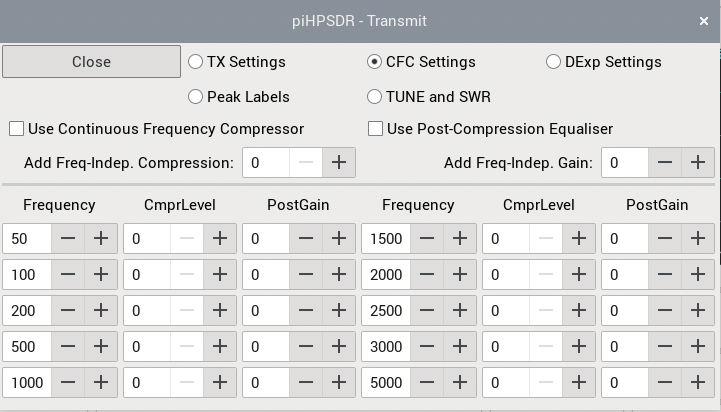
\includegraphics[scale=0.45]{TX_CFC.png}
\caption{The TX menu with the CFC settings}
\label{fig:CFCmenu}
\end{figure}

In the CFC sub-menu, the settings for the continuous frequency compressor can be made.
As the name indicates, the compression can be chosen frequency dependent. As for the
equaliser, one can specify corner frequencies with a given compression, between corner
frequencies the compression is interpolated linearly. In addition, there is an equaliser that
is applied after compression, so one give a gain (or attenuation) for each corner
frequency, with linear interpolation in-between. Gains in this menu are in dB and
can be chosen between -20 and +20 dB, compression levels are also in dB and can be chosen
between 0 dB (no compression) and +20 dB.

\rett{Use Continuous Frequency Compressor}. This checkbox is used to enable/disable the CFC. As with
the speech processor, using the CFC automatically enables the TX auto-leveller but note CESSB
overshoot control is \textit{not} enabled automatically.

\rett{Use Post-Compression Equaliser}. This checkbox is used  to enable/disable the post-compression
equaliser.

\rett{Add Freq.-Indep. Compression} With this spin button, one can specify an \textit{additional}
frequency-independent compression that applies to all frequencies.

\rett{Add Freq.-Indep. Gain} If using the post-compression equaliser, this spin button specifies an
\textit{additional} frequency-independent gain applied to all frequencies.

In the lower part of the menu, you find ten groups of three spin buttons that specify a frequency/level/gain
triple. The compression level and gain given (if the post-compression equaliser is used) applies to that
corner frequency while linear interpolation is used between corner frequencies.

\subsection{TX Menu: DEXP Settings}
\label{sec:dexp}

\begin{figure}[ht]
\center
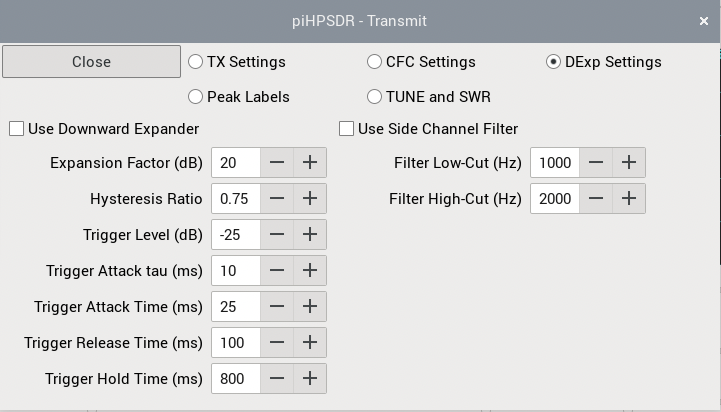
\includegraphics[scale=0.45]{TX_DEXP.png}
\caption{The TX menu with the DEXP settings}
\label{fig:DEXPmenu}
\end{figure}

In the sub-menu for the downward expander, you can control the settings for the downward expander
(DEXP). This can be viewed
as a configurable noise gate that applies to the TX audio input. Its main use is to suppress low noise
(e.g. from fans) that are taken up  by the microphone in speech pauses. The downward expander damps
such noise as long it is below a trigger level. Once the ,,noise'' exceeds the trigger level (that is,
the  operator speaks the next word or so) this damping is switched off. Sometimes, the ,,noise'' is
rather loud, such that noise alone leads to triggering, and in many cases such noise has rather low
frequencies. This is where a side channel filter comes in: this filter specifies a range of frequencies
used for triggering. For normal human voice for example, one expects that frequencies between 1000 and
2000 Hz are contained therein so one can only use these for triggering.

\rett{Use Downward Expander} With this check box, the DEXP can be enabled or disabled.

\rett{Use Side Channel Filter} With this check box, the side channel filter can be enabled of disabled.
With the  side channel filter enabled, only TX audio in the defined frequency  range will trigger the
noise gate.

\rett{Expansion Factor (dB)} This factor (in dB!) determines how strongly the noise will be damped as long
as it is below the trigger. The default (20 dB) should be OK in most cases.

\rett{Hysteresis ratio} If this  value is smaller than 1 (say, 0.75), then the hold time (the time in which the noise
gate is open starts when the input level drops below the trigger level, multiplied with the hysteresis ratio.

\rett{Trigger level (dB)} This spin button specifies the trigger level. It is given in dB relative to
full-amplitude audio samples. The default level (-25 dB, corresponding to an amplitude of 0.056) should
be OK in most cases.

\rett{Trigger Attack tau (ms)} This is the time constant (in ms) for averaging the input signal before
it goes to the detector.

\rett{Trigger Attack Time(ms)} This is the time used for opening the noise gate. To avoid plops in the
audio, the gate is not opened instantly but with a raised cosine characteristic. This time should not
be overly long, since otherwise parts of the first word spoken by the operator can get rejected by
the gate.

\rett{Trigger Release Time (ms)} This is the time used for closing the noise  gate. To avoid plops in the
audio, the gate is not opened instantly but with a raised cosine characteristic. The time for closing the
gate can usually be chosen much larger than for  opening.

\rett{Trigger Hold Time (ms)} After the operator has finished his speaking, the noise gate remains open
for some time (e.g. waiting for the next word). Typical hold times are of the order of 1 second, when no
new triggering audio arrives within that time, the gate is closed and the noise  thus suppressed.

\rett{Filter Low-Cut (Hz)} and \rett{Filter  High-Cut (Hz)} specify the frequency edges of the side
channel filter (if it is enabled). The defaults given here (1000--2000 Hz) are well suited  for distinguishing
human voice from humming noise coming from fans etc.

\subsection{TX Menu: Peak Labels}

The ``Peak Labels'' sub-menu allows one to control if and how labels
(values in dBm) are printed at the most prominent peaks on the
TX panadapter (Fig. \ref{fig:TXPeakMenu}):

\begin{figure}[ht]
\center
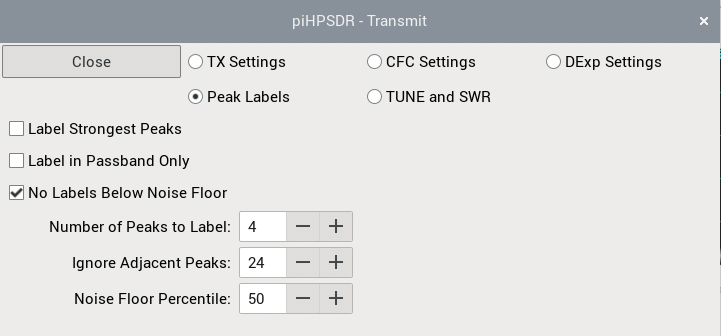
\includegraphics[scale=0.45]{TX_PEAK.png}
\caption{The TX menu with the peak label settings}
\label{fig:TXPeakMenu}
\end{figure}

\rett{Label Strongest Peaks} This enables peak detection and labelling.

\rett{Label in Passband Only} If the box is checked only the peaks within the
current filter pass-band  are shown.

\rett{No Labels Below Noise Floor} This suppresses labelling of peaks below the noise floor.

\rett{Number of Peaks to Label:} Set maximum number of peaks to be shown. There can always be less,
but no more than this number. The strongest peaks will be labelled first.

\rett{Ignore Adjacent Peaks:} Determine how close two peaks can be such that both are labelled.
The higher the number the closer the peaks can be to each other. It's a divisor of the
full window width so setting it to 1 will mean only one peak can occupy the entire window,

\rett{Noise Floor Percentile:} This is the percentile setting that defines the noise floor. If the
percentile is 50, then the noise floor is the level of that pixel that is in the middle of the list
if all pixels are sorted by their dBm value (a safety margin of 3 dBm is added).
If the \rett{No Labels Below Noise Floor} box is ticked
peaks below this value will not be labelled.

\subsection{TX Menu: TUNE and SWR}
This sub-menu allows to specify the TX drive level while TUNE-ing. For HPSDR radios which report forward
and reverse power (and thus the SWR), some SWR-dependent controls are added as well.

\begin{figure}[ht]
\center
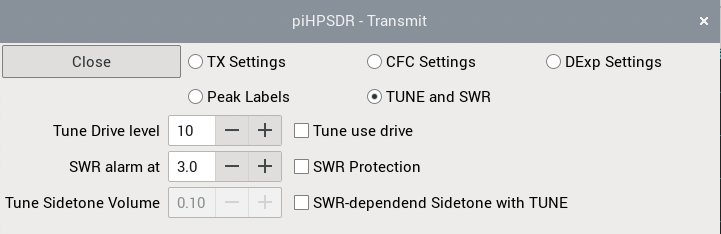
\includegraphics[scale=0.45]{TX_TUNE.png}
\caption{The TX menu TUNE/SWR settings}
\label{fig:TXTUNEMenu}
\end{figure}

\rett{Tune use Drive} If this box is checked, TUNE-ing will be done with the power that corresponds to the
current position of the drive slider, and the tune drive level is ignored.

\rett{Tune Drive Level} The value that can be adjusted with this spin box is the virtual position of the
drive slider while TUNE-ing. This value is ignored (and the spin-button made inactive)
if the \rett{Tune use Drive} box is checked.

\rett{SWR protection} If this box is checked, a very simple SWR protection is enabled. If the SWR exceeds
the threshold value (see next point), the drive slider is set to zero. The SWR protection is disabled
while TUNE-ing.

\rett{SWR alarm at} The spin button to the right determines the SWR threshold. If the SWR is beyond the
threshold, the SWR reported in the meter turns red. If SWR protection is enabled, the drive slider is set to
zero if the SWR exceeds the threshold.

\rett{SWR-dependent Sidetone with TUNE} If this box is checked, there will be a side tone while TUNE-ing.
This side tone is similar to a string of dots or dashes, separated by pauses which are 50 msec long.
The SWR is encoded both in the length and the frequency of the "dashes".  The higher
the SWR, the higher (with a limit of 5000 Hz) the pitch, an ideal 1:1 SWR results in a minimum pitch
of 500 Hz. Likewise, the "dot/dash" length is 50 msec for this ideal SWR and becomes longer as the SWR
gets larger. So for ideal SWR, the side tones sounds like a string of CW dots at 24 wpm at a pitch of
500 Hz. This ``dot length'' increases to 125 msec (with a pitch of 725 Hz) if the SWR is 1:1.5,
and to 500 msec (with a pitch of 1400 Hz) for an SWR of 1:3. The idea of
this feature is that one can operate a manual antenna tuner without looking at the screen.

\rett{TUNE Sidetone Volume} With this spin-button, one can adjust the volume of the SWR-dependent TUNE side tone
(allowed range: $0 \ldots 0.5$). \textbf{Attention!} Always start with small values to protect your ears.
This spin-box is inactive is the \rett{SWR-dependent Sidetone with TUNE} is not active.

%%%%%%%%%%%%%%%%%%%%%%%%%%%%%%%%%%%%%%%%%%%%%%%%%%%%%%%%%%%%%%%%%%%%%%%%%%%%%%%%%%%%%%%%%%%%%%%%%%%%%%%%%%%%
\clearpage
\section{The \texttt{PA} Menu}

In the \bltt{PA} menu, you can adjust the output level of your HPSDR board
to the PA being used, and you can establish a calibration of the
power that is displayed in the meter section while transmitting.
The menu presents itself as shown in Fig. \ref{fig:PAMenuCalibrate}.

\begin{figure}[ht]
\center
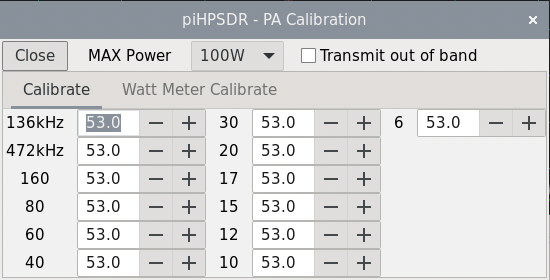
\includegraphics[scale=0.45]{PAmenuCalibrate.png}
\caption{The PA menu, PA calibration screen}
\label{fig:PAMenuCalibrate}
\end{figure}

In the first line, you can choose the maximum PA power of your
radio. The available values are 1, 5, 10, 30, 50, 100, 200, and
500 Watt. If your radio has a different maximum power, choose the
next largest value. The choice of this value only affects the
watt meter calibration (see below). If the  box
\rett{Transmit out of band} is checked, this allows \pH
to go TX if you are outside of the amateur radio bands.



\textbf{PA calibration.} If the \rett{Calibrate} sub-menu is active
(as shown in Fig. \ref{fig:PAMenuCalibrate}) you can adjust your
HPSDR board to your PA. This has to be done for each band separately,
and you need a dummy load and a watt meter to do so. Most watt meters
used by radio amateurs are not highly accurate, so if you can borrow
an accurate one, do so. The PA calibration values are the fictive
amplification of the PA. If the value is \textit{increased},
\pH assumes a higher amplification and will thus \textit{decrease}
the output power of the HPSDR board. Thus, \textit{increasing} the
PA calibration value will \textit{decrease} the output power. A calibration
value of 38.8 dB corresponds to the maximum RF output of the HPSDR board,
so the allowed range of values starts at 38.8.

To start calibration, go to the \bltt{TX} menu and check the
box \rett{Tune use Drive}. Then, hit the rightmost toolbar button
until one of these buttons reads \bltt{TUNE}. This way, when
TUNE-ing, you send a carrier with the power according to the drive
slider. For each band, go to the middle of the band, open the PA
menu, put the drive (\rett{TX Drv} slider) at 50 and hit the TUNE button. If the
output (measured with the Watt meter) is higher than half
of your nominal PA power, increase the
PA calibration value of that band, otherwise decrease it. Choose
a value such that your Watt meter reads half the nominal output
power. For fine adjusting, move the drive slider to 100 and
adjust the PA calibration value until your Watt meter shows the
nominal output  power. The calibration values will  (slightly)
differ from band to band, often one needs smaller values for the
higher bands since the amplification of the PA is smaller there.
If transverter bands have been defined via the \bltt{XVTR} menu,
they will also show up in this menu. Note that the PA calibration
value affects the level of the low-power TX output of the HPSDR board
an thus affects both the PA output (if the PA is enabled) as well
as the low-power TX output (if the Xvtr port is active as RX antenna).

\textbf{Watt meter calibration.} When PA calibration is complete,
you can calibrate the power reading within the meter section of
the \pH window. If you open the \bltt{PA} menu and click
on the text \rett{Watt Meter Calibrate}, the menu changes
and looks like in Fig. \ref{fig:PAMenuWatt}.

\begin{figure}[ht]
\center
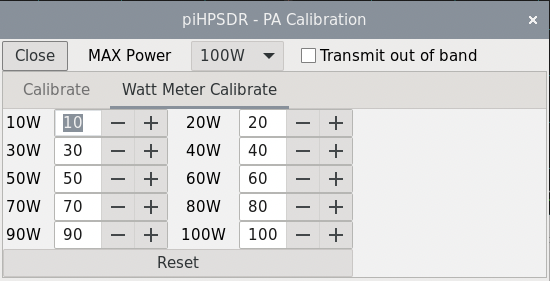
\includegraphics[scale=0.45]{PAmenuWatt.png}
\caption{The PA menu, Watt meter calibration}
\label{fig:PAMenuWatt}
\end{figure}
Note that for calibrating the Watt meter as well,
\rett{Tune use Drive} in the \bltt{TX} menu must be checked
to allow for high RF output
power while TUNE-ing.

You have 10 Watt values from $\frac{1}{10}$ to the full nominal power. Initially,
the values of the spin buttons beside the Watt ratings have the nominal value.
The calibration values can always be re-set to these nominal values by hitting
the \rett{Reset} button. Watt meter calibration is not done separately for all
bands, so it is suggested to perform the following procedure on the 20m band.
\pH will convert the ,,measured'' into the ,,reported'' value by linear
interpolation between two adjacent calibration values.

Start with resetting the value by hitting the \rett{Reset} button. Then, move the
drive slider to 100 (the unit of the drive slider is per cent, not Watt!) and hit
\texttt{TUNE} in the toolbar.
After the PA calibration described above, your (external) Watt meter should
show the nominal PA output power (e.g. 100 Watt for an Anan-7000). Now look at the
forward power reported in the meter section (top right of the \pH window).
Suppose you read "250 W" there although your output is 200 Watt. Then simply
insert the number 250 in the spin button to the right of the string
\rett{200W}. Now your watt meter reading should be close to 200W, you can fine-tune
it with the spin button. Note that \textit{increasing} the calibration value
with the spin button will \textit{decrease} the power indicated in the meter section.

You will observe that the calibration values for the lower powers also have changed.
This only happens if you start from nominal calibration values and change the
calibration value of the highest power. For example, if you have entered 250 in
the 200W spin button, then the value in the 100W spin button will read 125. So in a
single shot, you have roughly calibrated the Watt meter.

A finer calibration only makes sense if you have a highly accurate Watt meter, since
the (uncalibrated) reading in \pH may actually be more accurate than your
Watt meter. Using your highly accurate Watt meter,
you can now move the drive slider until your Watt meter exactly reads one of the
lower power values, and use the corresponding spin button to change the calibration
until \pH exactly reports the correct power.
The procedures is  virtually the same if our nominal output power is different.
The only complication arises if your radio has a nominal power that is not in the menu,
for example 150 Watt.

In this case, choose 200W (the next largest value)
in the top line of the PA menu. TUNE and move the drive
slider until your Watt meter reads the largest value possible that occurs
in the Watt meter calibration menu (in this example, it is 140W). Adjust the
140W spin button until \pH reports 140 Watt. Then go to full power
(150W) and adjust the 200W spin button until \pH reports 150 Watt.
Then, proceed with 120, 100, 80, etc. Watts.

%%%%%%%%%%%%%%%%%%%%%%%%%%%%%%%%%%%%%%%%%%%%%%%%%%%%%%%%%%%%%%%%%%%%%%%%%%%%%%%%%%%%%%%%%%%%%%%%%%%%%%%%%%%%
\section{The \texttt{VOX} Menu}

VOX (voice control) means that you can just speak into the microphone and the
radio goes TX, without the need to press a PTT button. VOX can also be used
in digital modes, if there is no possibility that the digi-mode program can
put \pH into TX mode via CAT commands or hardware lines. The VOX menu
is shown in Fig. \ref{fig:VOXMenu}.

\begin{figure}[ht]
\center
\includegraphics[scale=0.45]{VOXMenu.png}
\caption{The VOX menu}
\label{fig:VOXMenu}
\end{figure}

With the \rett{VOX Enable} check box, you can enable/disable VOX. For VOX operation,
there are two parameters, namely the VOX threshold and the VOX hang time. The VOX threshold
is the microphone amplitude required to trigger a RX/TX transition. If the radio goes TX
when the neighbour's hound starts barking, then the VOX threshold is too small. If the radio
does not go TX  although you speak loudly into the microphone, the threshold is too large.
The VOX menu features an indicator which can be green or red (in Fig. \ref{fig:VOXMenu}, this
is the green bar). This indicator flashes red if the microphone amplitude is above the VOX
threshold. Adjust the threshold with the slider such that the indicator becomes red if  you
speak into the microphone, but stays green if you don't speak.

The VOX hang time determines how long the radio stays in TX mode after the last time the
microphone delivered a signal that was above the VOX threshold. Typical values are 250 to
500 ms. If your radio produces relay chatter because it goes RX between your words,
increase the hang time. However, this will also increase the turn-around between you finished
your message and go RX.

VOX is very nice for rag-chew phone QSOs, I won't recommend it for contest operation.

%%%%%%%%%%%%%%%%%%%%%%%%%%%%%%%%%%%%%%%%%%%%%%%%%%%%%%%%%%%%%%%%%%%%%%%%%%%%%%%%%%%%%%%%%%%%%%%%%%%%%%%%%%%%
\section{The \texttt{PS} (PureSignal) Menu}

\begin{figure}[ht]
\center
\includegraphics[scale=0.45]{PSMenu.png}
\caption{The PureSignal (PS) menu}
\label{fig:PSMenu}
\end{figure}

PureSignal is the ,,street name'' for adaptive pre-distortion. What this means is, that
the signal from the \textit{output} of the PA (the ,,antenna signal'') is coupled
back (through an attenuator of typically 40-60 dB) to the radio and is analysed
whether is looks like it should. If it is distorted (e.g. by non-linearity of the PA),
then the PureSignal algorithm calculates how an input signal to the PA should look like
to produce the desired output. This is usually measured and calibrated with a so-called
two-tone experiment. In this experiment, two constant carriers, for example 7100 kHz
and 7101 kHz, are transmitted. If both carriers contain 25W power, this is
a 100W PEP signal. Non-linearity of the PA first lead to the occurrence of harmonics
(in this case around 14.2, 21.3, and 28.4 MHz). This is not a problem because
such harmonics are  damped by the TX low-pass filters. Higher-order non-linear effects,
however, lead to additional in-band signals, in our example they occur at
7102/7099, 7103/7098 etc. kHz. The low-pass filters cannot eliminate these signals,
they lead to unwanted signals (,,splatter'') that disturb QSOs on neighbouring
frequencies. With PureSignal, you can greatly reduce these unwanted signals.
If you open the \bltt{PS} menu for the first time it looks like shown in Fig.
\ref{fig:PSMenu}.



The elements have the following function:

\rett{Enable PS}. With this check box, PS can be enabled/disabled.

\rett{Two Tone}. With this button, a two-tone experiment can be started/stopped. The button
will be highlighted as long as the two-tone signal is transmitted. In the lower side band
modes (LSB, DIGL, CWL), an RF two-tone signal with frequencies 700 and 1900 Hz
\textit{below} the dial frequency are transmitted, in all other modes the two
RF frequencies are 700 and 1900 Hz \textit{above} the dial frequency. The same two-tone
experiment can be started/stopped via the toolbar, or by a GPIO- or MIDI-monitored
push button. At the beginning of a two-tone experiment, the diagnostic fields
are cleared and re-populated once a valid calibration has been obtained.

\rett{Auto Attenuate}. This enables/disables automatic adjustment of the RF input
attenuator to give the feedback level the correct strength. It is highly recommended
to use this option.

\rett{OFF}. With this button, the PS correction can be stopped (the \rett{status} will
then change to RESET).

\rett{Restart}. With this button, the PS correction can be resumed, for example after
it has been stopped.

\rett{MON}. With this button, it can be chosen whether the TX spectrum scope shows
the signal sent to the PA (MON button not highlighted) or whether the feedback signal
from the antenna is shown (MON button highlighted). Note that feedback data is only
available if PURESIGNAL is enabled. Without PS being enabled, the TX pan-adapter will
show the TX signal as it leaves \pH no matter if \rett{MON} is checked or not.

\rett{PS Feedback ANT}. Here it must be specified which antenna jack is used for the
PS feedback signal. It can be \rett{Internal} which means internal feedback
(for example as built into the Anan-7000 or  simply the cross-talk from the
TX/RX relay), or it can be \rett{Ext1} or \rett{ByPass} which refers to the
auxiliary antenna jacks.

\rett{PS MAP}. This box controls the PURESIGNAL ,,Map mode'' and is normally checked.
According to the WDSP manual, changing the Map mode allows easier calibration in
situations where a very poor PA is driven into heavy gain compression. The state
of this box has
no effect if there is no compression. \textit{PS is stopped and re-started if
this box is changed.}

\rett{PS Relax Tolerance}. This box is normally unchecked which means that the default
value 0.8 is used for the PURESIGNAL calibration tolerance. If checked, this tolerance
is reduced to 0.4. According to the WDSP manual, relaxing the tolerance my be helpful
for PAs with a very poor load regulation in the power supply such that there are
severe and slow memory effects. \textit{PS is stopped and re-started if
this box is changed.}

\rett{OneShot}. This box is unchecked by default. In the default case, the PURESIGNAL
algorithm constantly compares the transmitted and the feedback signal and thus
constantly updates the calibration. If \rett{OneShot} is checked, the calibration
is kept when the two tone experiment is finished. There are cases, especially if
CPU power is lacking, where the PURESIGNAL algorithm from time to time fails to obtain
a valid calibration, and when this happens during transmitting, a bad signal may
be transmitted for a short amount of time. Checking \rett{OneShot} can help in such
situations because the calibration, once obtained, is kept and not changed.
When a successful "one shot" PURESIGNAL calibration has been achieved, the \bltt{status}
field in the menu becomes stable and reads \texttt{STAYON}.

However, if something changes (e.g. output power, or the finals get warm, etc.) the
calibration is probably no longer valid but still kept. So unless you have good reason,
do not use the \rett{OneShot} option.


\rett{Feedback Lvl}. When doing a PS calibration through a two-tone experiment, this string
turns red if the feedback level is good. It turns yellow if the feedback level is slightly
to weak and read if it is too weak. A blue colour indicates a too string feedback level.
The feedback level reported by the PS calibration algorithm is further reported in the
,,feedbk'' field. The optimum value is about 154.

\rett{Correcting}. When doing a PS calibration through a two-tone experiment, this string
is green if calibration was successful and PS correction takes place, and the string is
red if no good calibration could be made.

\rett{TX ATT}. This element can occur both as a text field or as a spin button.
If PURESIGNAL is enabled while \rett{Auto Attenuate} is not enabled, it is a spin button with which
you can manually adjust the RF attenuation. For normal HPSDR radios, this is a value
between 0 and 31, other radios such as the HermesLite have an extended range from
-29 to 31. If the feedback level is too strong, this value must be increased, if it
is too strong, it must be decreased. It is, however, recommended to enable \rett{Auto Attenuate}.
In this case, the \rett{TX ATT} just shows the current attenuation.
Note that if \texttt{PURESIGNAL} is not enabled, the RF input attenuators
will automatically be set to maximum attenuation while transmitting with the PA enabled.

\rett{SetPk}. This field shows the currently assumed value of the peak value of the TX DAC
feedback signal. \pH chooses is automatically, depending on the radio hardware.
The standard value for Protocol-1 and Protocol-2 radios are 0.407 and 0.290. Notable exceptions are
the HermesLite-II running Protocol-1 (SetPK=0.240) and the Anan-G2 running Protocol-2 (SetPK=0.612).
The SetPK value is determined by the FPGA firmware of the radio can can experimentally
be determined by comparing the outgoing TX and the incoming TX feedback signal.
It should match the value reported
by the calibration algorithm in the GetPk field. You can change the value in the SetPk
field, the changed value is then also written to the props file and then restored
upon the next program start. This should only be done if the radio hardware has
a non-standard peak TX DAC value. One case I  know of is the "Brick2 SDR", which identifies
itself as a HERMES board but needs a quite large SetPk value of about 0.7800. But such
cases are easily identified when performing a two-tone test by a large difference
between the values in the SetPk field and the GetPk value which is obtained from analysing
the TX DAC data.

\textbf{Attention!} Specifying a wrong value in the \rett{SetPk} field will effectively
disable \texttt{PURESIGNAL}, and since this value is stored in the props file, this
adverse effect also shows up in the future, that is, until either the props file is deleted
or the correct value is again entered in the \rett{SetPk} field. This \textit{caveat} also
applies if you upgrade your radio firmware from protocol-1 to protocol-2, since then your props
file still contains the correct protocol-1 value (0.4067) and you have
to manually modify the \rett{SetPk} value (in this case, to 0.2899).

\begin{figure}[t!]
\center
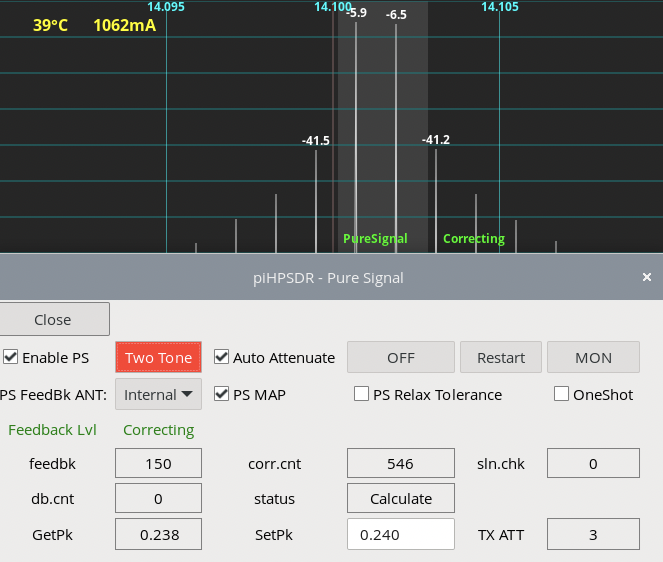
\includegraphics[scale=0.45]{PSnomon.png}
\caption{PS: TwoTone without MON}
\label{fig:PSnomon}
\end{figure}

If you want to use PURESIGNAL, it is required to enable PURESIGNAL by checking the
\rett{Enable PS} box, and it is recommended to use auto calibration (check the
\rett{Auto Attenuate} box). PURESIGNAL is then activated and calibrated by
performing a two-tone experiment. This can, but need not be, done by hitting
the \rett{Two Tone} button. PURESIGNAL restarting and calibration is also done
if a two-tone experiment is started via a GPIO/MIDI or toolbar button.
It is necessary to repeat such a two-tone experiment each time you change the
RF output power, since most likely a new TX attenuation value is needed. I also
recommend to repeat a two-tone experiment after each band change. If monitoring
the feedback signal (\rett{MON} button, this setting remains after closing the
PS menu) is enabled, a two-tone experiment also quickly shows how effective
the adaptive pre-distortion is. If everything works well, you only should see
two peaks on the TX pan-adapter during the two-tone experiment.

\begin{figure}[t!]
\center
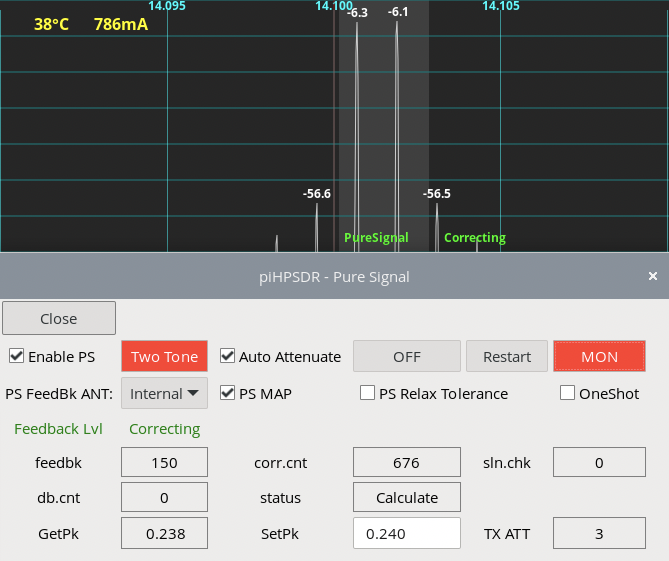
\includegraphics[scale=0.45]{PSmon.png}
\caption{PS: TwoTone with MON}
\label{fig:PSmon}
\end{figure}

\begin{figure}[t!]
\center
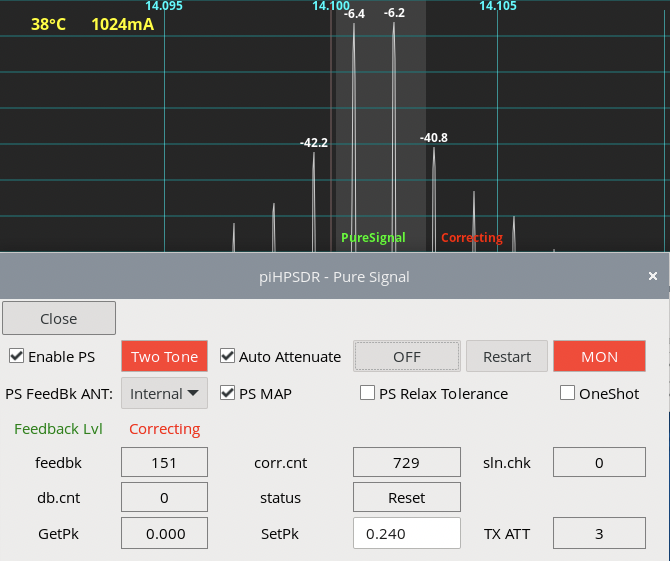
\includegraphics[scale=0.45]{PSoff.png}
\caption{PS: after hitting OFF}
\label{fig:PSoff}
\end{figure}

To demonstrate how PURESIGNAL works, I show an example performed with a Hermes\-Lite-II
radio running Protocol-1. The radio runs at a sample rate of 96 kHz, since it is my
experience that PURESIGNAL does not work too well in Protocol-1 when it is run
at 48 kHz. I also activated the optional ``peak labelling''
in the \bltt{TX Menu} such that the four main peaks heights are also printed
(in dBm) on the screen. Checking both \rett{Enable PS} and
\rett{Auto Attenuation}, and hitting the \rett{Two Tone} button, it needs only few
seconds to stabilise and then Fig. \ref{fig:PSnomon} results, where the TX
spectrum scope and the PS menu window have been arranged such that they do
not cover each other. Although both the PS menu and the spectrum scope state
that PS is working and correcting, the signal does not look good: a two-tone
signal should only have two peaks, but here one sees the two main peaks at $-7$ dBm
and two IM3 satellites at about $-43$ dBm (this amounts to an IM3 value of only $-36$ dBc).
The reason for this seemingly bad performance is of course, that the TX spectrum scope
normally shows the signal that is \textit{sent} to the PA, so we see a signal that
is distorted on purpose, and magically
exactly such that the PA makes a nice signal
out of this (\textit{adaptive pre-distortion}). If one wants to see what the antenna
is actually transmitting, one must
activate the \rett{MON} button such that it is highlighted.
This is shown in Fig. \ref{fig:PSmon}, where one sees the
feedback signal, that is, what the PA sends to the antenna.
This is a much cleaner two-tone signal (the IM3 value is about $-50$ dBc).
To demonstrate how effective the PS algorithm is,
I have pushed the \rett{OFF} button which stops the PureSignal correction, the result
is shown in Fig. \ref{fig:PSoff}. After hitting that button, IM3 satellites immediately
grow and IM3 decreases to
about $-35$ dBc which reflects the intrinsic
non-linearity of the PA.
Note that this is still a quite acceptable value.
Unless you have a class-A amplifier, your PA probably won't be much better.
This experiment demonstrates that adaptive pre-distortion is a mechanism that allows you to produce a clean
signal with a quality that would be impossible (or \textit{very} difficult) to achieve
with traditional hardware.

%%%%%%%%%%%%%%%%%%%%%%%%%%%%%%%%%%%%%%%%%%%%%%%%%%%%%%%%%%%%%%%%%%%%%%%%%%%%%%%%%%%%%%%%%%%%%%%%%%%%%%%%%%%%
\section{The \texttt{CW} Menu}
The CW menu controls parameters related to CW operation. The menu
is shown in Fig. \ref{fig:CWMenu}.

\begin{figure}[ht]
\center
\includegraphics[scale=0.45]{CWMenu.png}
\caption{The CW menu}
\label{fig:CWMenu}
\end{figure}

Many radios have a connection for a paddle or at least for
a straight key, and contain firmware to do CW. CW handling by
the radio firmware is enabled by the \rett{CW handled in Radio}
check box. If unchecked, CW (that is, generating and forming
the RF pulses) is done by \pH. For most radios, you can
still use the Morse paddle connected to the radio since the
radio sends the dash/dot paddle press events to the host
computer, but it is more versatile to connect
a Morse paddle, straight key or an external keyer is connected
to the host computer (see Appendix \ref{sec:ConnectCW}).

\rett{CW Speed}. Here the speed (in wpm) can be chosen. If CW is
handled in the Radio, the value is simply sent to the radio firmware,
which implements the (iambic) keyer. If CW is done within \pH,
this value is used by \pH's built-in iambic keyer. If using
a straight key, or an external keyer whose output is then treated
like a straight key, the speed has no meaning.

In either case, this speed is operative when sending CW text via
CAT commands (KY command), and it can also be changed by CAT
(KS command).

\rett{CW Break-In} This implements some sort of ,,CW-VOX''. In
break-in mode, the radio is automatically switched to TX when
a key or paddle is pressed. The delay, to be set by the spin
button to the right, is the time the radio goes RX after the
last Morse key closure.

\rett{Sidetone Level}. This is the level of the side tone,
either generated by the radio (if CW is handled there and the radio
has an audio codec) or
by \pH (if CW is not handled in the radio). The allowed range
is 0--127, typical values are between 10 and 20. The side tone level
is usually set to zero if, for example, a low latency side tone is
produced outside \pH. In this case, one usually wants to hear
the tone from CAT CW messages being sent, so if the side tone is
zero, a default side tone level (12) is used while transmitting
via CAT.

\rett{Sidetone Freq}. This is the frequency of the side tone and the
,,BFO offset''. That is, if a CW signal is received exactly at the
dial frequency, the CW audio signal has this pitch. Note that unless
one uses XIT, the transmitted CW signal is exactly on the VFO dial
frequency as well.

\rett{Weight:} If using a iambic keyer (either in the radio or
the builtin keyer), this value (0-100) determines the dash/dot ratio.
The normal value is 50, which means that a dash is three times longer
than a dot. The dash length is proportional to this value, so it can
be from zero to six times the dot length.

%\rett{CW ramp width (ms)}. This spin-box lets you choose the
%width of the ,,ramp'' used for RF CW pulses.
%At the beginning of a dot or dash, the
%amplitude of  the RF pulse is slowly
%increased from zero to full amplitude at the beginning,
%and at the end the amplitudes slowly fall down to zero.
%This avoids harsh clicks in the RF signal
%(which could possibly been heard all over the band for
%hard keying). An optimised ramp function has been implemented
%that gives good click suppression both at small and large
%offsets from the carrier frequency. The
%width is the rise/fall time of the pulse envelope, using the default value
%(9 msec) you will meet ARRL's CSI (clean signal initiative) specification
%for all CW speeds up to 40 wpm. Ramp widths can be chosen from
%5 to 16 msec (\pH does not allow values smaller than 5 msec
%to ensure that your CW signal does not produce overly strong clicks).
%If the RF pulse is shaped
%by \pH (\rett{CW handled in Radio} \textit{not} checked),
%you will get
%the optimised ramp function an the chosen ramp width.
%A very recent Protocol-2 update
%(March 2024) allows to send the ramp width to the radio as well.
%However, the FPGA firmware in the radio will ignore that value
%unless you run a very recent model, so with
%\rett{CW handled in Radio} checked, changing the ramp width in this menu
%has possibly no effect.
%
%The CW side tone needs pulse shaping as well to become pleasant.
%To make sure that the delay of the CW side tone is
%as small as possible, a ramp with a raised cosine shape
%and a constant width of 5 msec (independent of the ramp width
%used for RF) is used when \rett{CW handled in Radio} \textit{not} checked
%such that \pH shapes the side tone.

\rett{Paddle Mode:} Here the choice is Iambic Mode A, Iambic Mode B,
and  Straight Key. In Straight Key mode, the key has to be connected
to the dash paddle, since the built-in keyer implements a bug mode
there (automatic dots from the dot paddle, straight key behaviour
for the dash paddle). When using an external keyer, use StraightKey
mode and connect the keyer output to the dash paddle input.

\rett{Enforce letter spacing}. This option forces you to give ,,cleaner'' CW
when in iambic mode. If at the end of an inter-element pause no key is
pressed, then there is a forced additional pause of two times a dot length. While this
prevents you from sending too short spaces between two letters, it
might well corrupt a letter you want to send. For example, when sending
the letter "X" and the dot paddle is pressed a little too late, you
instead send "TU". This option is probably more useful for practising than
for doing real QSOs.

\rett{Keys reversed}. When checking this box, the dot and dash contacts
are reversed, so you need not re-wire your paddle.


%%%%%%%%%%%%%%%%%%%%%%%%%%%%%%%%%%%%%%%%%%%%%%%%%%%%%%%%%%%%%%%%%%%%%%%%%%%%%%%%%%%%%%%%%%%%%%%%%%%%%%%%%%%%
%%%%%%%%%%%%%%%%%%%%%%%%%%%%%%%%%%%%%%%%%%%%%%%%%%%%%%%%%%%%%%%%%%%%%%%%%%%%%%%%%%%%%%%%%%%%%%%%%%%%%%%%%%%%
\chapter[Menus for RX and TX]{The Main Menu: menus for RX and TX}

\section{The \texttt{DSP} (Signal Processing) Menu}

\begin{figure}[ht]
\center
\includegraphics[scale=0.45]{DSPMenu.png}
\caption{The DSP menu.}
\label{fig:DSPMenu}
\end{figure}

The \bltt{DSP} menu sets parameters related to DSP (digital signal processing)
within the WDSP library.
Filter characteristics can be specified separately for the RX1 (and RX2, if
running two receivers) and TX (if the radio does have a transmitter)
filters. In addition, enabling/disabling binaural receiver audio
is done here.  Most users will
very rarely need to invoke this menu, which is shown
in Fig. \ref{fig:DSPMenu}.

\rett{Filter Type} (RX only). Digital filters can be designed such that a signal within the
pass band leaves the filter in a shape as similar as possible
to what went into the filter. This requires that the phase
difference between input and output signal is a linear
function of the frequency. Another desirable property
of a linear filter is that the time delay between a signal
going into a filter and what comes out is as small as
possible. Unfortunately there some sort of uncertainty
relation between these two properties, so you only can
trade one for the other. The options for the filter type
are thus \rett{Linear Phase} or \rett{Low Latency}.
But note that there is a lot of latency in the HPSDR data
processing which you cannot avoid, so ,,low'' latency
is not really low. Therefore, the default option
is \rett{Linear Phase}, and there should be little reason
to change this. Note that \pH does not allow low latency
filters for TX, since in this case the TX compressor
could not be used with the CESSB overshoot correction.

\rett{Filter Size}. This is the number of ,,taps'' of the digital
filter. Increasing this size will inevitably increase the latency,
but makes the filter edges steeper. The allowed values are
powers of 2, and the minimum value equals the buffer size, which
is hard-coded in \pH to be 1024 (except for the transmitter in Protocol-2,
where it is reduced to 512). The default value of 2048 should be
fine in almost all cases, if you increase it, you can notice that
the filter edges become little more ,,brick wall'' like.

\rett{Binaural} The RX audio signal by default is a mono signal. Although
you have the RX audio signal on both ears if using a headphone, both the
left and right channel are the same. Checking \rett{Binaural} for a
receiver implies that its RX audio signal is stereo (left and right channel
differ). This is accomplished by copying the primary I and Q signal of the
RX output to the left and right channels instead of using the I signal
for both ears (which is the default). Some users report that in modes
such as CW and SSB, binaural audio is more pleasant than the default.
It is up to the user to try and set this parameter according to personal
preferences. This checkbox is available for all receivers but not for the
transmitter.

%%%%%%%%%%%%%%%%%%%%%%%%%%%%%%%%%%%%%%%%%%%%%%%%%%%%%%%%%%%%%%%%%%%%%%%%%%%%%%%%%%%%%%%%%%%%%%%%%%%%%%%%%%%%
\section{The \texttt{Equaliser} Menu}
\label{sec:eqmenu}

In the \bltt{Equaliser} menu, you can modify the frequency response of
the RX and TX audio. You can adjust the RX equaliser to your personal
preferences for listening to the RX audio. The TX equaliser affects
your transmitted signal. You can, for example, provide some extra
amplification to the low-frequency part of your voice. The menu
is shown in Fig. \ref{fig:EqualiserMenu}.

\begin{figure}[ht]
\center
\includegraphics[scale=0.45]{EqualiserMenu.png}
\caption{The Equaliser menu}
\label{fig:EqualiserMenu}
\end{figure}

With the radio buttons in the top row you can select
whether you want to control or modify the equaliser settings for the receivers
RX1 or RX2, or for the transmitter. If only one receiver is running,
the \rett{RX2 Settings} button does not appear. Likewise, if the radio
has no transmitter, the \rett{TX Settings} button does not appear.

Below the  top row, there are the controls that affect the equaliser
that has been selected there.
The \rett{Enable} checkbox enables/disables the equaliser.
If the equaliser of the active receiver
is enabled, the EQ indicator in the
VFO bar, upon receiving, turns yellow and reads \rett{RxEQ}.
If the TX equaliser is enabled, this indicator turns yellow
while transmitting and reads \rett{TxEQ}. So while receiving,
you cannot tell, from the VFO bar, whether the TX equaliser is
actually enabled or not!

The spin button \rett{Added Frequency-Independent Gain} specifies
an \textit{additional} gain (or attenuation) applied to all frequency
channels. Gains in this menu are in dB and can vary from -20 to +20,
-20 is of course  not a ,,gain'' but an attenuation by 20 dB.

In the bottom part of the menu, there are ten pairs of spin buttons
that specify 10 corner frequencies and the gains associated therewith.
This defines the 10 channels
of the equaliser. Note frequencies may appear in any order since they
are sorted before the equaliser settings are updated. Note however,
if you specify a frequency twice with two different gains, the outcome
is undetermined.

The gain at one of the   corner frequencies is exactly the gain
chosen by the spin button (plus any frequency-independent gain
selected by the spin button in the second row). Between two
corner frequencies, the gain is frequency dependent and obtained
by liner interpolation between the two corners. For a frequency
between  zero and the lowest corner frequency, the gain chosen for that corner
frequency applies, and likewise the gain selected for the largest corner frequency
applies to all frequencies above that frequency.

Equaliser settings are saved with the mode, so
if you adjust the equalisers when doing USB or LSB, and then switch to
DIGU or DIGL, the equaliser settings for DIGU/DIGL become effective
(normally, equalisers are disabled for digital modes).
They resume their USB/LSB
settings upon switching back to USB or LSB. This also applies to other
modes such as CWU/CWL, where the TX equaliser has no meaning
anyway, and where the RX equaliser is normally not needed.

%%%%%%%%%%%%%%%%%%%%%%%%%%%%%%%%%%%%%%%%%%%%%%%%%%%%%%%%%%%%%%%%%%%%%%%%%%%%%%%%%%%%%%%%%%%%%%%%%%%%%%%%%%%%
\section{The \texttt{Ant} (Antenna) Menu}

The \bltt{Ant} menu, as shown in Fig. \ref{fig:ANTmenu},
applies to HPSDR radios. For SoapySDR radios, the layout
is much simpler because there are much fewer choices possible.

\begin{figure}[ht]
\center
\includegraphics[scale=0.45]{ANTmenu.png}
\caption{The ANT (antenna) menu.}
\label{fig:ANTmenu}
\end{figure}

Standard HPSDR radios have, in most cases, three main antenna jacks
denoted \rett{Ant1}, \rett{Ant2}, \rett{Ant3}, which can be used both for receiving to
the first ADC and
transmitting. Then there are up to additional antenna jacks (\rett{Ext1}, \rett{Ext2},
and \rett{Xvtr}) which can only be used for receiving and are also connected
to the first ADC. If the radio has more than one ADC, the (RX only)
antenna jack, usually denoted RX2, is hard-wired to the second ADC.

If the menu is opened, the \rett{HF} button is checked, and the HF bands
are displayed. The WWV and general ,,bands'' are on display as well so you
can e.g. choose an antenna for listening to signals outside of
the amateur bands.
If one checks the \rett{XVTR} button, the transverter bands
are shown (this leads to an empty window if no transverter bands have
yet been defined), and one can go back to the HF bands by re-checking
\rett{HF}.
For each band, one can now choose one (out the three) antennas for
transmitting and one (out of six) antennas for receiving. The main purpose
of this is the possibility to connect an additional receive-only antenna
such as a beverage antenna which often has a better signal-to-noise
ration than standard antennas used for transmitting.

\textbf{Transverter operation.} Newer radios (Anan-7000, 8000, and Saturn/G2) have a
switchable low-power TX output, e.g. the \texttt{Xvtr Out} jack at the Anan-7000 back plane.
This output is automatically enabled if \rett{Xvtr} is selected as the RX antenna of RX1.

\begin{center}
\fbox{
\parbox{\textwidth - 1cm}{
\begin{center}
\textbf{\color{red} -------- Attention, potential damage! --------}
\end{center}
A problem that may potentially damage your external hardware occurs if
you use one of the antennas Ant1/2/3 for receive and another for transmit.
This is especially true if you have sensitive hardware (such as an
active RX antenna) connected to
the Ant jack used for RX and operate CW with the Key attached to the radio
with the \rett{CW handled in Radio} box checked in the \bltt{CW} menu.

In this case, starting CW transmission lets the FPGA (processing unit
inside the radio) put the
radio into TX mode, start forming the first RF pulse, and informs the
host computer running \pH that a RX/TX transition has been made.

Only then, \pH can start telling the radio to switch the relays that
connect the Ant jacks with the TX circuitry.

As as result, a small part (few ms) of the first RF pulse (dot or dash)
may appear at the Ant jack used for RX only. If, say, an active antenna is
connected there, this may well destroy the active antenna.

Even if not using CW this way, it cannot excluded that Ant relay switching
is so slow that such ,,RF spikes'' appear at an Ant jack intended for RX
only.

A very recent (Jan 2024) update of the Protocol-2 definition offers the possibility to
tell the radio which antenna settings is must use when it goes TX on its
own behalf. \pH fully supports this, and if you have an updated
Protocol-2 firmware in your radio then the problem disappears. For Protocol-1,
there is no such update so the problem remains.

\vspace{0.5cm}
\textbf{If possible, use the Ext1/Ext2/Xvtr jacks for connecting sensitive equipment.}
}
}
\end{center}


%%%%%%%%%%%%%%%%%%%%%%%%%%%%%%%%%%%%%%%%%%%%%%%%%%%%%%%%%%%%%%%%%%%%%%%%%%%%%%%%%%%%%%%%%%%%%%%%%%%%%%%%%%%%
\clearpage
\section{The \texttt{OC} (Open Collector) Menu}

\begin{figure}[ht]
\center
\includegraphics[scale=0.45]{OCMenu.png}
\caption{The OC (open collector) menu.}
\label{fig:OCMenu}
\end{figure}

Standard HPSDR radios have seven individually programmable outputs wired as
open collector output. In the \bltt{OC} menu, you can specify, separately
for each band, and separately for receive and transmit, which output should
be ,,set''. This can be used to switch the band filters of an external PA
or of an external RX pre-selector, to control an automatic antenna tuner,
and many more things, since it is
your external hardware which in the end has to make sense of the output
bit pattern.

For non-HPSDR radios, the \bltt{OC} menu does not appear in the main menu. Since
transverter bands are also shown at the bottom of the list, the \bltt{OC}
menu may become rather high, in this case its height is restricted to the
screen size and a vertical scroll bar is added.

To facilitate control of an automatic tuner, there are seven \rett{TuneBits}
which are OR-ed with the bit pattern chosen for TX on the actual band,
as long as you are TUNE-ing with \pH. Besides the \bltt{Tune} command,
there are the \bltt{Tune Full} and \bltt{Tune Mem} commands which are
functionally equivalent, except that the open collector tuning pattern
is removed for \bltt{Tune Full} after the full tune delay, and for \bltt{Tune Mem}
after the memory tune delay, which can also be specified in this menu.
This can be used to send tuning pulsed of varying length to the
external automatic tuner at the beginning of the tuning. If the open collector
outputs are not used, or if the \rett{TuneBits}  are all unchecked, there is
no functional difference between the \bltt{Tune}, \bltt{Tune Full} and
\bltt{Tune Mem} commands.

The \bltt{OC} bit pattern you see in Fig. \ref{fig:OCMenu} is what you automatically
get when selecting the
\texttt{N2ADR} filter board in the \bltt{Radio} menu
(this is usually the
case if you are working with a HermesLite-II radio). This means that
you \textit{can} change the \bltt{OC} patterns when using the \texttt{N2ADR} filter board
(e.g. for experimental purposes), but
these changes are lost once you select another filter board and then select \texttt{N2ADR} again,
and also upon the next program start.

%%%%%%%%%%%%%%%%%%%%%%%%%%%%%%%%%%%%%%%%%%%%%%%%%%%%%%%%%%%%%%%%%%%%%%%%%%%%%%%%%%%%%%%%%%%%%%%%%%%%%%%%%%%%
%%%%%%%%%%%%%%%%%%%%%%%%%%%%%%%%%%%%%%%%%%%%%%%%%%%%%%%%%%%%%%%%%%%%%%%%%%%%%%%%%%%%%%%%%%%%%%%%%%%%%%%%%%%%
\chapter[Controlling \pH]{The Main Menu: controlling \pH}

In this chapter, the customisation of the toolbar (at the bottom of the \pH window),
as well as how to configure GPIO and MIDI controllers, is described. Furthermore, in this
chapter we discuss the \bltt{CAT} menu which allows controlling \pH by some external program
such as a logbook or contest program, via standardised CAT commands that can be sent to
\pH either over a serial line or via TCP. If TCI is enabled at compile  time, this menu
is called \bltt{CAT/TCI} and also allows to control the built-in TCI server.

\textbf{Note for Controller1 owners:} The eight switches (push-buttons) of the controller,
that a positioned below the screen, are bound to the eight toolbar buttons on the screen.
Therefore, there is no "Switches" menu for this controller, and the switches are implicitly
configured via the Toolbar menu.

\begin{figure}[ht]
\center
\includegraphics[scale=0.45]{ToolbarMenu1.png}
\caption{The Toolbar menu, just opened.}
\label{fig:ToolbarMenu1}
\end{figure}

\section{The \texttt{Toolbar} Menu}
\label{sec:toolbarmenu}
We start with the "Toolbar" menu, that can be found at the top of the rightmost
column in the main menu. The toolbar consists of eight buttons that can be assigned
to a set of eight functions. There are six such sets, and pressing the rightmost button
of the toolbar cycles through these six sets. The text on the rightmost toolbar button, \rett{FNC(0)}, indicates which
layer is currently active.

\begin{figure}[ht!]
\center
\includegraphics[scale=0.45]{ToolbarMenu2.png}
\caption{Toolbar menu. Changing third button in \texttt{F1} layer.}
\label{fig:ToolbarMenu2}
\end{figure}

If the \bltt{Toolbar} menu is opened, it looks like Fig. \ref{fig:ToolbarMenu1}.
The rows correspond to the six different layers, and the rightmost button in each
row indicates to which layer this row belongs.
If one now clicks (just an example)
the \texttt{CTUN} button (third button in the second row) a ,,command dialog'' pops up that looks as
in Fig. \ref{fig:ToolbarMenu2}.


\begin{figure}[ht!]
\center
\includegraphics[scale=0.45]{ToolbarMenu3.png}
\caption{Just selected \texttt{Band20}.}
\label{fig:ToolbarMenu3}
\end{figure}

The current command selected (\texttt{CTUN}) is high-lighted. Lists of possible commands can be rather long,
so it might be necessary that you have to scroll up or down in such an command dialog until you have
found what you were looking for. Now (again just an example) the button \texttt{Band 20} has been clicked
in the command dialog, such that it gets high-lighted (Fig. \ref{fig:ToolbarMenu3}).

If one now closes the command dialog by clicking the \texttt{OK} button, the command select menu
closes and on sees that in the toolbar menu now reappearing (Fig. \ref{fig:ToolbarMenu4}), the third button
in the second
line of the toolbar menu has changed, it now gives the short text (\texttt{20}) of the command, which will
switch the active receiver to the 20m band (see the explanation of all the commands in Appendix A).

\begin{figure}[ht!]
\center
\includegraphics[scale=0.45]{ToolbarMenu4.png}
\caption{Toolbar assignment accomplished.}
\label{fig:ToolbarMenu4}
\end{figure}

You also see that the toolbar itself has not changed, because we have just changed the \texttt{FNC(1)} set,
while currently the \texttt{FNC(0)} set is active. If one now, however, clicks the rightmost
toolbar button with the text \texttt{FNC(0)} one advances to the next set and the toolbar labels
are updated (Fig. \ref{fig:ToolbarMenu5}).

\begin{figure}[ht!]
\center
\includegraphics[scale=0.45]{ToolbarMenu5.png}
\caption{The new \texttt{F1} layer is operative.}
\label{fig:ToolbarMenu5}
\end{figure}

It can be seen that the text of the first seven toolbar buttons has changed to reflect
the functions of the \texttt{F1} set, and also the rightmost button (which is always mapped
to \bltt{Function}) has changed to \texttt{FNC(1)} in order to indicate the \texttt{F1}
layer is now active. For mouse users (only), a secondary click on the rightmost toolbar
button cycles through the layers in in reverse order.

Note that it is not possible to change the assignment of the  rightmost button of the toolbar,
it will always be assigned to \bltt{Function}, since if one has no access to this
function, one is stuck and can no longer cycle through the function layers.

%%%%%%%%%%%%%%%%%%%%%%%%%%%%%%%%%%%%%%%%%%%%%%%%%%%%%%%%%%%%%%%%%%%%%%%%%%%%%%%%%%%%%%%%%%%%%%%%%%%%%%%%%%%%
\section{The \texttt{CAT/TCI} Menu}

\pH has a built-in rig control or CAT (computer aided transceiver) facility. This can be used to control
\pH from other programs or even other computers. You can have up to three simultaneous CAT connections
via TCP, and three additional CAT connections via serial lines (provided the host computer running \pH
has those serial interfaces available). Note that on the new Anan G2-Ultra radios, one of the serial lines
is used for controlling the front panel.
It is also possible to use FIFOs (also known as named pipes) instead of real serial devices, which offers a
hardware-free connection
of, say, a logbook program running on the same computer to \pH, even if the logbook program cannot use
TCP. On my Macintosh computer for example, using a named pipe and the Kenwood TS-2000 radio model,
I can connect the MacLogger DX logbook program with \pH.
\pH fully supports (thanks Rick!) the ANDROMEDA controller (see \texttt{github.com/laurencebarker/
Andromeda\_front\_panel}).
This controller (or rather the Arduino inside) is connected to the host computer via USB and appears as a
USB-to-serial
device on the host computer. The CAT command set is explained in Appendix \ref{sec:catcommands}. In most
cases, using
the Kenwood TS-2000 as the radio model would do it, if the digi mode or laptop program uses the
\texttt{hamlib} library  to interface with
radios, either choose TS-2000 or (preferably) the ,,OpenHPSDR PiHPSDR'' radio model because this
uses time-out values adapted to \pH.

If compiled  with TCI  support, \pH also offers a (substantially  stripped-down) TCI server, and in this
case this menu is named \bltt{CAT/TCI}. \pH cannot
be \textit{controlled} via TCI (all incoming TCI commands are  ignored) but it periodically (every 500 msec)
reports operating frequencies  and modes, if they have changed. This is meant  to support  logbook programs
and external PAs that use TCI  to get frequency and/or mode information.

The \bltt{CAT/TCI} menu is shown in Fig. \ref{fig:CATmenu}. Note that if \pH  is  not compiled
with TCI support,  this menu is simply called  \bltt{CAT} and lower part  of the menu is not shown.

\begin{figure}[ht]
\center
\includegraphics[scale=0.45]{CATmenu.png}
\caption{The CAT/TCI  menu.}
\label{fig:CATmenu}
\end{figure}

\rett{Enable CAT/TCI Debug Logging}. If enabled, the \pH CAT subsystem sends lots of debug messages to the standard output. If
\pH is run
from within a terminal window, these messages appear in the terminal window. If it is run from double-
clicking a desktop icon,
these messages can be found in a log file within the \pH working directory (this is the directory where
the preferences
are stored. This checkbox is only of interest for software developers to analyse programming or connection
errors, and should
not be checked for normal use.

\rett{TCP}. This sets the TCP port number for CAT connection to TCP. The default value (19090)
is rather standard, using another one is only necessary if you are running more than one
SDR program on the host computer at the same time.
This port number must match the port number used in the (digi-mode or logbook) program that wants to connect.

\rett{Serial}. \pH support up two three CAT connections over serial lines or named pipes.
In the text field, enter the device name of the serial port or the named pipe to use.
Which names to use
is highly operating system dependent. On a RaspPi,  USB-to-serial
adapters (which are nowadays the standard way to add serial ports to a computer) have names such as
\texttt{/dev/ttyACM0} or \texttt{/dev/USB0} (on RaspPi) or \texttt{/dev/tty.usbserial-....} (on MacOS).
On Anan G2-Ultra radios, a serial line is used for the communication with the front panel. This
port is detected automatically and the third "Serial" line done not contain any controls but simply
states the auto-detected port name and whether the connection to the panel has been successfully
established.


To the right of the serial port text field, there is a pop-down menu for choosing the baud rate. Only 4800,
9600, 19200, and 38400 baud are offered, but this should cover most cases.

\rett{Enable}. This checkbox enables or disables the \pH CAT subsystem for that particular case.
Enabling and disabling can be done separately for the TCP CAT subsystem, for each of the serial
CAT connections, and the TCI server.

\rett{Andromeda}. This checkbox enables the TCP or  serial CAT connection for use with ANDROMEDA consoles
of the G2-MkII front panel. Serial lines are
forced to 9600 baud if enabled for ANDROMEDA. Furthermore, status changes of \pH (e.g. RIT on/off) are
automatically reported via ZZZI CAT commands (see Appendix \ref{sec:catcommands}). These messages are
used by the ANDROMEDA console or the G2-MkII front panel
to switch LED indicators such that they reflect the current state
of \pH. Note that the \rett{Andromeda} flag is only inspected when the connection is opened. Serial CAT connections
are established when successfully opened upon program start or via this menu.
TCP CAT connections are established when the \textit{client} successfully connects.

\rett{AutoRprt}. If a CAT connection (either via TCP or via a serial line) is opened and this box is checked,
the connection is put in ,,auto reporting'' mode. This mode can generally be enabled and disabled with the
ZZAI or AI CAT commands (see Appendix \ref{sec:catcommands}), but with this checkbox, the connection can be put
into ``level 1'' auto reporting mode without the CAT client sending AI commands. ``Level 1'' means that \pH
behaves as if an \texttt{AI1;} or \texttt{ZZAI1;} command had been received. In this level, frequency changes
are transmitted via FA and FB CAT messages, but mode changes are not transmitted.
The main use for auto reporting mode is, if a buggy power amplifier or a buggy logbook program
is connected via a serial line that needs frequency or mode  info via CAT but fails to send a proper
\texttt{AI} command.  If you do not have hardware that depends
on such unsolicited (without requesting them via ZZAI or AI commands) messages, this box should never be checked.

\rett{TCI}. To the right of this string, there is a spin button which selects the TCP port used by the
TCI  server (the default value is 40001). The TCI server identifies itself as an ExpertsSDR3 program
running TCI version 1.8 with a SunSDR2PRO radio, but in fact it ignores all incoming commands and only
reports VFO-A/B frequencies and modes, if they have changed. It also reports the TX frequency if it has changed.
This is necessary since the TX frequency can jump from the VFO-A to the VFO-B frequency and back e.g. when
changing the split status or the active receiver.

\rett{Report TX  Frequency Only}. If power amplifiers connect to \pH, they usually only want to know the
TX frequency to adjust the output low-pass filters. Checking this box restricts the TCI outgoing commands
to the TX  frequency messages. It is important  to note that the TX frequency is only  checked every
500 msec, so after a band change, the PA may  not be aware of  the changed TX frequency for half  a second.


%%%%%%%%%%%%%%%%%%%%%%%%%%%%%%%%%%%%%%%%%%%%%%%%%%%%%%%%%%%%%%%%%%%%%%%%%%%%%%%%%%%%%%%%%%%%%%%%%%%%%%%%%%%%
\section{The \texttt{MIDI} Menu}
\label{sec:midimenu}
MIDI (musical instrument digital interface) is a protocol designed for the communication of
musical instruments, such as keyboards and tone generators. Because of its widespread use,
support in all major operating systems, and it inherent ability to deliver real-time ,,events'',
it is also an ideal protocol to control an SDR program. The only MIDI messages \pH processes
are NoteOn, NoteOff, and ControllerChange messages. Typically, a NoteOn message is sent if
a key on a keyboard is hit. The first parameter of a NoteOn/Off message is the key
it refers to. Although keyboards rarely have more than 88 keys, the allowed range for
the key is 0-127. There is an additional parameter (,,velocity'', range 0-127) that tells how
fast the key has been hit (this makes the difference between a soft and loud tone on the piano).
NoteOn/Off messages are ideally suited for indicating button press and release events. In principle,
\pH does not need the velocity. However, several MIDI consoles, in a sloppy interpretation of
the MIDI standard, send a NoteOn value with zero velocity if a button is released. Therefore,
\pH interprets a NoteOn message with a velocity different from zero as a ,,button press'',
and interprets both a NoteOn messages with zero velocity and a NoteOff message as a ,,button release''.

The original MIDI standard was built upon a daisy-chained serial connection. Each device
echos all messages it receives at its input side to the output. Therefore, a key-down
message that originated on one keyboard is sent to all tone generators. Likewise, a tone
generator receiving a key-down message cannot tell from which device the message
was originally sent. To resolve possible conflicts, each MIDI message contains a channel
number. There is some confusion about channel numbers: the MIDI says channel numbers
go from 1 to 16. Because this is encoded in a 4-bit data field whose numerical value
goes from 0 to 15, computer users normally refer to channel numbers from 0 to 15,
and this convention is also followed by \pH. Different channel numbers can be used
to discriminate MIDI events from different sources (devices). An example of such a setup
is if you connect a DJ console as well as a micro controller to which a CW key is attached.

The second type of messages are ControllerChange messages. Typically, they report the value of
an expression pedal, if it has changed. A ControllerChange message also has two parameters,
namely the number of the controller (0-127) and the value (0-127). A ControllerChange
message could be sent if the MIDI controller has a potentiometer, to report its position,
encoded from 0 (full counter clock wise) to 127 (full clock wise). Such a message could then be
used to control in \pH, say, the AF volume or the TX drive. Such a potentiometer is
not suited to become a ,,VFO knob''. Here one uses rotary encoders, a piece of hardware which
you can turn (as long as you like) in either direction, and which reports (by hardware pulses)
how fast and it which direction it is turned. Unfortunately, there is no standard how to
encode these increments into MIDI ControllerChange messages. My Behringer CMD-PL1 console,
for examples, uses ControllerChange numbers 65, 66, 67, $\ldots$ for clockwise rotations
and 63, 62, 61, $\ldots$ for counter clock wise rotations, and further encodes the speed of
rotation in how far the value differs from 64. Other brands interpret the 7-bit number
as a signed quantity, such that values 0, 1, 2, $\ldots$ correspond to clockwise,
and numbers 127, 126, 125, $\ldots$ to counter-clockwise rotations. It is clear that
the \pH MIDI configuration menu must be flexible enough to handle all these situations.

\begin{figure}[ht]
\center
\includegraphics[scale=0.45]{MIDImenu1.png}
\caption{The (virgin) MIDI menu.}
\label{fig:MIDImenu1}
\end{figure}

From this it is clear that within \pH, we have to distinguish three types of sources
of MIDI commands:

\rett{KEY}. This type is generated by NoteOn/Off MIDI events. \pH commands (,,Actions'') that
can be assigned to this type are typically those which can also be assigned to toolbar
buttons.

\rett{KNOB/SLIDER}. This type is generated by ControllerChange MIDI events. It can be used
for \pH functions that are usually controlled by a slider, such as adjusting the AF
volume, setting the TX drive, setting the AGC gain, etc.

\rett{WHEEL}. This type is also generated by ControllerChange MIDI events. This means
that if such an event is configured, the user has to decide whether this event
originated from a potentiometer or from a rotary encoder. The prototypical \pH
function controlled by a WHEEL is a VFO knob, which you can spin forever. However,
you can also assign to to the AF volume control. \pH takes care that the
AF volume stops at the extreme cases (-40 and 0 dB for AF volume) even if you continue
spinning.

The first kind of MIDI device which is often used for SDRs are the so-called MIDI DJ
consoles. If you search the internet for ,,Hercules DJ controller'' or ,,Behringer
DJ controller'' you will find lots of examples. For a very decent price, you
can obtain a device which features lots of controls which you can conveniently use
as VFO knobs, smaller knobs for controlling the AF volume etc., and push buttons
to be used, for example, instead of toolbar buttons. The second kind of MIDI devices
are small MIDI-capable micro controllers, starting with Teensy and Arduino devices
which have a 32U4 micro controller which has built-in MIDI capability. With such a
micro controller, you can build your own "DJ controller". Let the 32U4 control
lots of push buttons and rotary encoders, and send the MIDI messages via USB to the
computer. Using such a micro controller is also the most convenient and general way
to connect a Morse key or paddle to the host computer running \pH (see
Appendix \ref{sec:ConnectCW}, you can but need not use the same micro controller
for taking care of the buttons/encoders and the CW key).

If you open the \bltt{MIDI} menu for the first time, it presents itself as shown
in Fig. \ref{fig:MIDImenu1}.



At the top of the menu, besides the close button, you find a list of MIDI devices
in the system, each of which with a check box. In Fig. \ref{fig:MIDImenu1}, there is only
one such device with name ,,CMD PL-1 MIDI 1''. You will find all MIDI devices attached
to the host computer here. With the check box(es), enable those you want to use.
This way it is possible to run two instances of \pH on the same computer, both
connected to different radios, and control them independently with two different MIDI
consoles. The first thing you have to do is to check all MIDI devices you want to use.

\rett{Ignore Controller Pairs}. This check box  which is unchecked by default
The MIDI standard offers the possibility to combine two controllers, one
(primary one) in the range 0--31 and the other (auxiliary one)
with a a controller number larger by 32, thus in
the range 32--63. The value of the auxiliary controller is then interpreted as a
fine resolution correction of the value of the primary controller. Technically
speaking,
a pair of ControllerChange events sets a 14-bit value for the lower controller.
Some MIDI consoles
from the music market (for example, the Hercules DJ200 controller)
use this mechanism. \pH, especially the MIDI menu, gets confused
by these "controller pairs". Checking the \rett{Ignore Controller Pairs} box just tells
\pH to ignore MIDI ControllerChange event if the controller number is between 32 and 63.
As a consequence, only the most significant 7 bits of the 14-bit value are used, which
is fine for most applications.

\begin{figure}[ht]
\center
\includegraphics[scale=0.45]{MIDImenu2.png}
\caption{The MIDI menu, VFO wheel turned.}
\label{fig:MIDImenu2}
\end{figure}

It is important to note that as long as the MIDI menu is open, the radio cannot be
operated through MIDI since all MIDI messages are captured by the menu and
displayed. This is used to implement a ,,self-learning'' configuration. To explain
this in detail, we demonstrate how to configure MIDI such that the big wheel on the
controller is used as a VFO knob. After I have activated the checkbox of our
MIDI device, I just turned the big wheel of the MIDI console a bit. This resulted
in a menu window that is shown in Fig. \ref{fig:MIDImenu2}. In the third line,
below \rett{Event}, you see \texttt{CTRL} which indicates that the last MIDI messages
received was a ControllerChange message. In the case of a NoteOn/Off messages, this
field would read \texttt{NOTE}. You should rotate the knob in both directions to
see what happens: below \rett{Value} the ControllerChange value of the latest
message is recorded, while the \rett{Min} and \rett{Max} fields report the smallest
and largest value seen (all in the range 0-127). By playing around, it became
quickly clear that this is a rotary encoder, sending messages in the range 65, 66, 67,
$\ldots$ for clockwise rotation and values 63, 62, 61, $\ldots$ for counter clockwise
rotation. If it were a potentiometer, you would see values between 0 and 127
depending on the position of the potentiometer.

Below \rett{Channel}, you see the value zero which
indicates that the channel number of that MIDI message was 1 (see above on the
different channel numbering). Below \rett{Type}, you see a pop-down menu, here
you can choose between \rett{WHEEL} and \rett{Knob/Slider}. In the example shown,
it must be a \rett{WHEEL} since this is a rotary encoder. Because there is no
standard how the values map to increments, a separate panel
\rett{Configure WHEEL parameters} pops up when a wheel is to be configured.
Here one has to define ranges of values that apply for very fast left turns,
fast left turns, normal left turns, normal right turns, fast right turns,
and very fast right turns. Specifying an interval from $-1$ to $-1$ means that
this case will never be realised. In the example shown (Fig. \ref{fig:MIDImenu2}),
we have chosen to map all values from 0-63 to a left turn, and all values from 65-127
to a right turn.
\begin{figure}[ht!]
\center
\includegraphics[scale=0.45]{MIDImenu3.png}
\caption{The MIDI menu, selecting VFO command}
\label{fig:MIDImenu3}
\end{figure}

\begin{figure}[ht!]
\center
\includegraphics[scale=0.45]{MIDImenu4.png}
\caption{The MIDI menu, VFO command selected}
\label{fig:MIDImenu4}
\end{figure}
Now we have to specify which \pH function should be triggered when moving the wheel.
The current command is shown in a button below the string \rett{Action} and defaults to \bltt{NONE}.
By clicking this button, a dialog to choose the function opens as described for the
\bltt{Toolbar} menu (chapter \ref{sec:toolbarmenu}), with the current choice (\bltt{NONE})
highlighted. The only difference is that now only functions are listed that can be
assigned to encoders.
Because we want to assign the wheel to the \bltt{VFO} function, we click
the \bltt{VFO} button, which then becomes highlighted (Fig. \ref{fig:MIDImenu3}).



Then one has to click the OK button to make the choice, and one returns to the
MIDI menu (see Fig. \ref{fig:MIDImenu4}).

One sees that the choice just made has entered the MIDI configuration, as documented by the
list in the bottom right part of the menu. At this stage, we can continue
assigning more encoders, potentiometers, or buttons. If we close the menu at
this point, then the big wheel on the MIDI console can immediately be used
to change the VFO frequency.

%%%%%%%%%%%%%%%%%%%%%%%%%%%%%%%%%%%%%%%%%%%%%%%%%%%%%%%%%%%%%%%%%%%%%%%%%%%%%%%%%%%%%%%%%%%%%%%%%%%%%%%%%%%%
\section{The \texttt{Encoders} Menu}
\begin{figure}[ht!]
\center
\includegraphics[scale=1.00]{g2_frontpanel.png}
\caption{A picture of the (first generation) G2 front panel (image courtesy of Apache Labs).}
\label{fig:g2_frontpanel}
\end{figure}

\begin{figure}[ht]
\center
\includegraphics[scale=0.45]{EncoderMenuG2.png}
\caption{The Encoder menu for the G2 front panel controller}
\label{fig:EncoderMenuG2}
\end{figure}
The \bltt{Encoders} menu can be used to assign functions to the encoders of a
GPIO-based controller, that is, either a
Controller1, Controller2 or the G2 front panel of the first-generation Anan-G2 radios
(those without LEDs and a 7-inch screen). For the second-generation G2 radios
(``G2 Ultra'') with LEDs and an 8-inch screen in the panel, see the \bltt{G2panel}
menu, chapter \ref{sec:G2panelMenu}.

This implies that this menu is only available if \pH has been compiled with GPIO support,
and if furthermore on the initial (discovery) screen one of the controllers mentioned above have
been selected. Note further that the ,,large knob'' of these controllers
cannot be assigned a non-default function, this knob is hard-wired to the \bltt{VFO} function.


While the function of this menu is the same in all three cases (Controller1, Controller2,
G2 front panel), the layout is different, because the position of the menu buttons
are meant to indicate which encoder is referred to.



The G2 front panel (Fig. \ref{fig:g2_frontpanel}) has,
in addition to the large VFO knob at the bottom right,
four small knobs, two (one above the other)
at the left edge and two at the right edge. All four knobs are double encoders with
a switch. This means that there is an inner/upper knob (,,top encoder'')
and an outer/lower knob (,,bottom encoder''), which
are two separate encoders. Furthermore, you can push the knob and have and additional
push button function (,,Switch''). If you open the \bltt{Encoders} menu for
a G2 front panel controller, the menu opens as shown in Fig. \ref{fig:EncoderMenuG2}.
You see four groups with three buttons (Switch, Top, Bottom) each, and it should be
clear which group belongs to which encoder. With the buttons, you can choose which function
to assign, in the same way as described for the \bltt{Toolbar} (chapter \ref{sec:toolbarmenu})
and \bltt{MIDI} (chapter \ref{sec:midimenu}) menus. With the \rett{Default} button, you can
re-assign the default values (those shown in Fig. \ref{fig:EncoderMenuG2})
to the encoder functions, which match the silk printing
on the enclosure (see Fig. \ref{fig:g2_frontpanel}).

\begin{figure}[ht!]
\center
\includegraphics[scale=0.8]{Apache_Controller2.png}
\caption{A picture of the Controller2 (image by courtesy of Apache Labs).}
\label{fig:Apache_Controller2}
\end{figure}

The Controller2 (see Fig. \ref{fig:Apache_Controller2}
has (besides the VFO knob at the bottom right) three knobs (arranged horizontally) at the bottom left,
and a fourth knob at the top right, all of which are double encoders with a switch.
So if you run \pH with a Controller2, then the menu looks different (Fig. \ref{fig:EncoderMenuV2}).
The menu shows
for groups with three buttons each, and it should be clear which group belongs to which button. The
\rett{Default} button again re-installs the default functions (those shown in Fig. \ref{fig:EncoderMenuV2}).

\begin{figure}[ht!]
\center
\includegraphics[scale=0.45]{EncoderMenuV2.png}
\caption{The Encoder menu for Controller2}
\label{fig:EncoderMenuV2}
\end{figure}

\begin{figure}[ht!]
\center
\includegraphics[scale=0.75]{Apache_Controller1.png}
\caption{A picture of the Controller1 (image by courtesy of Apache Labs).}
\label{fig:Apache_Controller1}
\end{figure}


Finally, the Controller1 (see Fig. \ref{fig:Apache_Controller1})
has (besides the big VFO knob at the bottom right)
three knobs (denoted E1, E2, E3), arranged vertically at the right edge. These knobs
are single encoders with a switch (you can turn the knob, but you can also push it). Therefore,
the \bltt{Encoders} menu in this case (Fig. \ref{fig:EncoderMenuV1}) shows three groups with
two buttons each. The \rett{Default} button again re-installs the default values shown in
Fig. \ref{fig:EncoderMenuV1}, these are chosen just for convenience since there are no default
function printed on the enclosure.

\begin{figure}[ht!]
\center
\includegraphics[scale=0.45]{EncoderMenuV1.png}
\caption{The Encoder menu for Controller1}
\label{fig:EncoderMenuV1}
\end{figure}

\clearpage
%%%%%%%%%%%%%%%%%%%%%%%%%%%%%%%%%%%%%%%%%%%%%%%%%%%%%%%%%%%%%%%%%%%%%%%%%%%%%%%%%%%%%%%%%%%%%%%%%%%%%%%%%%%%
\section{The \texttt{Switches} Menu}

he \bltt{Switches} menu can be used to assign functions to the encoders of a
GPIO-based controllers Controller2 or the G2 front panel of the first-generation Anan-G2 radios
(those without LEDs and a 7-inch screen). For the second-generation G2 radios
(``G2 Ultra'') with LEDs and an 8-inch screen in the panel, see the \bltt{G2panel}
menu, chapter \ref{sec:G2panelMenu}.

This implies that this menu is only available if \pH has been compiled with GPIO support,
and if furthermore on the initial (discovery) screen one of the controllers mentioned above have
been selected. Note that this menu is also not available
for the Controller1 because the eight push buttons of this controller are hard-wired to
the toolbar buttons and their functions as thus assigned via the \bltt{Toolbar} menu
(see Chapter \ref{sec:toolbarmenu}).


On the G2 front panel (see Fig. \ref{fig:g2_frontpanel}),
there are a lot of push buttons: at the left edge, to the right
of the left edge encoders, are two buttons, at the bottom right, below the VFO knob,
there are two more buttons, and at the top right, to the right of the left edge
encoders, is an array of 12 (4x3) buttons. The layout of the \bltt{Switches} menu
for the G2 front panel (Fig. \ref{fig:SwitchMenuG2}) features (besides the Close
button) sixteen buttons, and their arrangement is such that you can easily guess
which menu button refers to which button on your G2 front panel. Assigning functions
to these buttons is done exactly as described for the \bltt{Toolbar} menu
(chapter \ref{sec:toolbarmenu}). With \rett{Default} one re-installs the default values
shown in Fig. \ref{fig:SwitchMenuG2} which match the functions printed on the enclosure.

\begin{figure}[ht]
\center
\includegraphics[scale=0.45]{SwitchMenuG2.png}
\caption{The Switches menu for the G2 front panel controller.}
\label{fig:SwitchMenuG2}
\end{figure}

The Controller2 (see Fig. \ref{fig:Apache_Controller2} in the last section)
also has 16 push buttons, but they are arranged differently:
at the bottom edge there are 7 buttons arranged horizontally. At the right
edge, there is an array of 8 buttons (4x2) with one additional button
above the right column that is to the right of the fourth encoder, just
below the power button. Looking at the \bltt{Switches} menu for the
Controller2 (Fig. \ref{fig:SwitchMenuV2}), you see representations of
these 16 buttons in an arrangement for which it is self evident which
menu button refers to which Controller2 push button.
Assigning functions
to these buttons is done exactly as described for the \bltt{Toolbar} menu
(chapter \ref{sec:toolbarmenu}).
With \rett{Default} one re-installs the default values
shown in Fig. \ref{fig:SwitchMenuV2} which match the functions printed on the enclosure.

\begin{figure}[ht]
\center
\includegraphics[scale=0.45]{SwitchMenuV2.png}
\caption{The Switches menu for Controller2.}
\label{fig:SwitchMenuV2}
\end{figure}
%%%%%%%%%%%%%%%%%%%%%%%%%%%%%%%%%%%%%%%%%%%%%%%%%%%%%%%%%%%%%%%%%%%%%%%%%%%%%%%%%%%%%%%%%%%%%%%%%%%%%%%%%%%%
\section{The \texttt{G2panel} Menu}
\label{sec:G2panelMenu}

\begin{figure}[ht]
\center
\includegraphics[scale=0.25]{g2ultra.png}
\caption{The front panel of a second-generation G2 radio(image courtesy of Apache Labs).}
\label{fig:g2ultrapanel}
\end{figure}

The \bltt{G2panel} menu becomes available as soon as the presence of a second-generation G2 front panel
(G2 Ultra or upgraded first-generation G2s) has been detected. These panels communicate with \pH through
a serial line connection using an ANDROMEDA-like protocol. Fig. \ref{fig:g2ultrapanel} shows the front
panel of a G2-Ultra. In contrast to a first-generation G2, it has an 8-inch screen and panel contains
several LEDs. The \bltt{G2panel} menu also applies to first-generation G2 radios with an upgraded
compute module running \pH. Part of such an upgrade is an additional micro controller that handles the
panel and communicates with \pH via a serial line connection.

Note that this menu cannot be used to assign a non-default command to the VFO knob.
After first opening the \bltt{G2panel} menu, it looks quite empty (Fig. \ref{fig:g2panelmenu-initial}):

\begin{figure}[ht]
\center
\includegraphics[scale=0.45]{g2panelmenu-1.png}
\caption{The \bltt{G2panel} menu, just opened.}
\label{fig:g2panelmenu-initial}
\end{figure}

As long as this menu is open, the front panel seems inoperative. The reason is, that all button and
encoder event are ``digested'' by the menu itself. As soon as a button is pressed or an encoder is
turned in either direction, the menu records which controller was last used, and reports the last
recorded action (either a button press or turning an encoder knob). For example, after pressing
the TUNE button, the menu changes to the following (Fig. \ref{fig:g2panelmenu-recorded}):

\begin{figure}[ht]
\center
\includegraphics[scale=0.45]{g2panelmenu-2.png}
\caption{The \bltt{G2panel} menu, reporting the last ``panel action''.}
\label{fig:g2panelmenu-recorded}
\end{figure}

So the menu states that the last ``panel action'' recorded was a button press (the internal code number
of the button is of little importance here), and that the \pH command assigned to this button was
\bltt{Tune}. Furthermore, once there has been communication between the panel and the \bltt{G2panel}
menu, a large button appears at the bottom of the menu which can be used to overwrite all button and
encoder assignments with the factory default.

I you wish to assign a new command to this button (it is the last button you have touched), simply
click into the button in the second line which states which command is currently assigned. In our
example, it is the button with the label \bltt{Tune}. Clicking this button opens the same
``action dialog'' already discussed in the previous sections. In this dialog, you can choose a
new command to be assigned with that button. In our example, I have chosen the \bltt{Cmpr On/Off}
command which switches TX compression on/off (Fig. \ref{fig:g2panelmenu-chosen}).

\begin{figure}[ht]
\center
\includegraphics[scale=0.45]{g2panelmenu-3.png}
\caption{The \bltt{G2panel} menu, reporting the newly chosen command.}
\label{fig:g2panelmenu-chosen}
\end{figure}

If one wants to assign new commands to other buttons or encoder, just press the button or turn the
encoder, and the menu will report a new ``last panel action'' and lets you assign a new command
to that button or encoder. If all assignments have been made, close the menu and the new panel
functions become operative.

Note that your assignments are permanent. They will be stored in the props file and be restored
the next time you start \pH. If you think your choices were not that clever, you can always go back
to the factory settings, which will then overwrite your personal assignments in the props file as well.

%%%%%%%%%%%%%%%%%%%%%%%%%%%%%%%%%%%%%%%%%%%%%%%%%%%%%%%%%%%%%%%%%%%%%%%%%%%%%%%%%%%%%%%%%%%%%%%%%%%%%%%%%%%%
%%%%%%%%%%%%%%%%%%%%%%%%%%%%%%%%%%%%%%%%%%%%%%%%%%%%%%%%%%%%%%%%%%%%%%%%%%%%%%%%%%%%%%%%%%%%%%%%%%%%%%%%%%%%
\chapter{Client/Server remote operation}
\label{sec:clientserver}

In client/server operation, two instances of \pH are running closely coupled. The ,,local'' \pH program
(called the server) runs as usual on a computer with direct network connection to the radio. This computer is usually located
in the vicinity of the radio. On the other hand, the ,,remote'' \pH program (called the client) my run
on a computer quite far away from the radio. Both instances of \pH are connected via a network connection
that may bridge a long distance. Wireless connection is perfectly possible between the client and the server.
The connection of the two \pH instances need much lower bandwidth as e.g. the server/radio connection.
The data stream from the server to the client is dominated by the RX audio samples,(48k 16-bit
stereo samples per second, or  1.5 MBit/sec) while the data stream from the client to the server requires
only half as much since the TX microphone samples are mono. Note the TX microphone samples are only sent
while TXing in modes other than CW, so no heavy protection/encryption is necessary: the data flowing is
essentially that what can be heard on the air anyway. The method of generating CW inside \pH has been
converted to a ,,time-stamped event model'', so sending CW is perfectly possible with remote operation.

Since this is a legal requirement in many countries, access to the server is password protected to prevent
illegal use of the transmitter. While the password is stored unencrypted on the server side, a challenge/response
model ensures that a non-encrypted password is never contained in the data stream connection the client and
the server.

In the \pH ``server`` instance (connected directly to the radio), client/server operation must be enabled
via the \bltt{Server} menu, to be opened by a button in the bottom  part of the leftmost  column of the  main menu.
The server menu is shown in Fig. \ref{fig:servermenu} and only has a few controls.

\begin{figure}[ht]
\center
\includegraphics[scale=0.45]{ServerMenu.png}
\caption{The \bltt{Server} menu}
\label{fig:servermenu}
\end{figure}

The \rett{Server Enable} check-box can be used to enable or disable remote operation. If the box is not
checked, a client cannot connect. The  spin-box  to the right of the \rett{Server Port} label lets the user
choose the TCP port to be  used for remote operation. This must be a port that is not yet used on the
computer running the \pH server instance. The default value 50000 works in most cases, but you can choose
another value should the port 50000 be in use on your computer. Other ports used by \pH are 19090 (the default
port for CAT-over-TCP) and 40000 (the default port for the TCI server).

In the text entry field to the left of   the \rett{Server Password} label, you must enter a password for
client-server operation. If it is a really long password, only the first 64 characters are used, and if it
is shorter than 5 characters, no client is allowed to connect. No particular security measure is taken
to protect the password on the server side: it is  shown while you type it into the  text field, and it is
stored in the local preferences file without encryption. The idea here is that you set up the server
in a private environment, and against those who manage to hack your computer running the \pH server instance
there is nothing one can do from within \pH.

Let us assume you have a server instance of \pH running, so how to connect  to it from a  remote location?
Here it is useful to show again the discovery menu on the \pH start screen (Fig. \ref{fig:clientmenu}):

\begin{figure}[ht]
\center
\includegraphics[scale=0.45]{ClientMenu.png}
\caption{The discovery menu on the client side}
\label{fig:clientmenu}
\end{figure}

Here, no local radios have been found as indicated in the first line. The second line contains the controls
relevant for  client/server operation. There is a pop-down menu to the right of the \rett{Use Server} button.
Here one has to specify the host address and port number of the server, address and port separated by a colon.
For the host address, on can use numerical IP addresses of the form xxx.xxx.xxx.xxx but equally well a
host name. The port number must, of course, match the port number specified in the \bltt{Server} menu in
the \pH server instance (see above).

In the \texttt{host:addr} pop-down menu, you can choose the entry matching your server. On a virgin system, this menu
will  only show a default entry which is 127.0.0.1:50000, and an empty entry. By clicking into the text field, you
can change an entry such that it matches for \pH server instance. You can also select the empty entry from
the pop-down menu and enter a new \texttt{host:addr} pair, which will then be added to the list.
 The last element of
the pop-down menu is always an empty one, so you can add as many different entries as you wish. If you select
an entry, click  into the text  field and clear it, then this entry is  removed from the pop-down menu.
In this way, you can configure your client computer to use several different \pH server instances, but also
to use a \pH server instance that has different IP addresses or host names depending from where you connect.

The second text field in the server line must be used to enter a password. This password will not be
stored in the preferences file so you have to enter it each time you connect (I might change this in the
future, but at the moment this seems to be the most secure option). By default, the last button in
the server line reads \rett{Show} and the password is hidden (each character is represented by a bullet).
If clicking the \rett{Show} button, its label changes to \rett{Hide} and the password becomes visible. You
might have guessed that clicking the \rett{Hide} button then conceals the password again and the button
label reads \rett{Show} again.

\clearpage
\textbf{A note on network security:}

The password you enter is \textbf{never ever} transmitted ``as is'' over the line. Instead, the server sends a random
512 bit (64 byte) \textit{challenge} which is different for each connection.
On the client side, a four-byte version number and the password is added
to the challenge and a SHA512 key is built from the result.  Using the last result as the new challenge,
this process is repeated 99999 times to make brute-force attacks compute intensive,
and the last hash generated is then sent back to the server. The server
does the same with its version number and the password entered in the \bltt{Server} menu and then asserts
that the two SHA512 keys are identical.
On a RaspberryPi5, generation of the hash takes about 120 msec, and about 3 times less on powerful desktop
computers. Once a hacker has ``sniffed'' a valid challenge/hash pair, trying to guess the password
from generating all possible hashes
from the challenge for, say, passwords of length 8 and consisting of lower-case letters and numbers only
(2.8 * 10$^{12}$ possibilities) will take about 10$^{11}$ seconds (3500 years) of CPU time, and better
passwords which also include upper-case letters are even better.
Although this still  not  top-notch cyber security, it should be good enough
to fulfil your  (legal) obligations as a radio amateur to prevent your gear from unlawful use.
If you feel you must go beyond, one option is to set up a VPN \textit{virtual private network} in which
you can have expert-level cyber security provided by your network infrastructure rather than by an application such
as \pH.

\textbf{Auto disconnect feature:}

Equally important is to prevent that your radio stops transmitting if
the connection to the client breaks down. To this end, the server closes the connection and goes RX if
it has not received any command from the client for about 30 seconds, or if the attempt to read the
next command from the client failed (the client will send a
``heartbeat'' message every 15 seconds).

\textbf{Network bandwidth required for client/server operation:}

 The user commands and even the spectrum
data to be displayed in the panadapters and waterfalls are the smallest part of the data flowing between the client
and the server. The (by far) largest part is the audio data. Audio data is transferred as signed 16-bit integers
at a sample rate of 48 kHz, in stereo for the RX audio (Server $\to$ Client) and in mono for the TX
microphone data (Client $\to$ server). During RX, and also during TX when doing CW, no TX microphone data
is transferred. If not using duplex, no RX audio data is transferred when TXing because the receivers are shut down.

This means that during RX, about 96 kByte/sec (768 kbit/sec) are transferred from the Server to the Client
(twice as much if running two receivers), while only half of this is transferred from the Client to the Server during
TX if doing SSB. When TXing in CW, very little data (the CW key-down/up time stamps) is actually sent from the client
to the server.
My first tests indicate that client/server operation works very well even
if parts of the connection between Client and Server
is using a WiFi. I mention this because my attempts using WiFi for connection to the \textit{radio}
(that is, for the base band IQ data) were not entirely satisfactory.
%%%%%%%%%%%%%%%%%%%%%%%%%%%%%%%%%%%%%%%%%%%%%%%%%%%%%%%%%%%%%%%%%%%%%%%%%%%%%%%%%%%%%%%%%%%%%%%%%%%%%%%%%%%%
%%%%%%%%%%%%%%%%%%%%%%%%%%%%%%%%%%%%%%%%%%%%%%%%%%%%%%%%%%%%%%%%%%%%%%%%%%%%%%%%%%%%%%%%%%%%%%%%%%%%%%%%%%%%
\chapter{Miscellaneous Topics}
There are several topics that are not best explained in the course of the \textit{tour de force} through
the menus. These will be handled in this section.

\section{RX/TX profiles}
\label{sec:rxtxprofiles}
Many settings such as VFO step sizes, filter choices, noise reduction
settings, equaliser settings, and TX compressor settings
are only reasonable for a specific mode and need be re-adjusted if one changes
the mode. For example, one might wish to use
different VFO step sizes for different modes, and get the step size chosen for that
mode automatically if one switches to that mode. The same applies to noise reduction
settings which are very different for CW and SSB. For digital modes (DIGU/DIGL),
one normally does not want neither noise reduction or equaliser being active on the RX
side, nor a speech processor for transmitting.

On the other side, one often wants the same settings for USB and LSB, or for DIGU and DIGL.
Therefore three mode groups have been defined that encompass USB/LSB/DSB, CWU/CWL, and
DIGU/DIGL. There are two more mode ,,groups'' with AM and FM  as the only one member.

Each mode  has an associated RX/TX profile containing lots of settings (see below).
When switching a mode (either by an explicit request, or implicitly by a VFO swap/copy
operation, a band or band stack change, or by recalling a memory slot), the profile of
that mode overwrites the current settings.

The RX/TX profile for a specific mode (group) is updated whenever one of the settings
contained in the profile is updated for RX1 or for the transmitter. Note that the
mode-specific RX/TX profile is also applied to RX2 if the mode of RX2 is changed,
but changing the settings for RX2 does not update the profile.

For example, if you have adjusted the noise reduction settings while operating USB,
these settings are stored in the RX/TX profiles of the USB, LSB, and DSB modes. Whenever
switching to USB, LSB or DSB in the future (until the profile is changed again), these
settings become active. So you can quickly cycle, say, between USB, CWU and
DIGU and upon each mode change you get the settings that you have chosen for that mode.

Here is the list of settings that form the RX/TX profile:

\begin{center}
\begin{tabular}{l}
\toprule
$\bullet$ VFO step size  \cr
$\bullet$ VFO RIT step size \cr
$\bullet$ RX Filter (which one to use) \cr
$\bullet$ RX CW peak filter (on/off) \cr
$\bullet$ RX Noise reduction (all settings) \cr
$\bullet$ RX Noise blanker (all settings) \cr
$\bullet$ RX Automatic notch filter (on/off) \cr
$\bullet$ RX Spectral  noise blanker (on/off) \cr
$\bullet$ RX AGC characteristic (slow/medium/fast etc.) \cr
$\bullet$ RX equaliser (all settings) \cr
$\bullet$ TX equaliser (all settings) \cr
$\bullet$ TX speech processor (on/off, compression level) \cr
$\bullet$ TX continuous frequency compressor (CFC, all settings) \cr
$\bullet$ TX downward expander (DEXP, all settings) \cr
$\bullet$ TX mic gain slider position \cr
$\bullet$ TX filter settings (low/high or use RX filter)\cr
\bottomrule
\end{tabular}
\end{center}
%%%%%%%%%%%%%%%%%%%%%%%%%%%%%%%%%%%%%%%%%%%%%%%%%%%%%%%%%%%%%%%%%%%%%%%%%%%%%%%%%%%%%%%%%%%%%%%%%%%%%%%%%%%%
\clearpage
\section{The TX audio chain}
\label{sec:txchain}
It seems that how the TX audio chain works is a field where myths and facts are equally dominant, therefore
this section tries to shed some light on this. We will discuss the most relevant parts of the TX
chain which process the input signal in the following order

\begin{itemize}
\item{The downward expander (DEXP)}
\item{The Mic gain slider (MicGain)}
\item{The equaliser (TXEQ)}
\item{The auto-leveller (AUTOLVL)}
\item{The continuous frequency compressor (CFC)}
\item{The speech processor (CMPR)}
\item{The controlled envelope SSB overshoot control (CESSB)}
\item{The automatic level control (ALC)}
\end{itemize}

In \pH, there are no user-accessible controls for AUTOLVL and CESSB as they are activated
automatically when appropriate (see below).

For digital modes, the input audio level is fairly constant and can be set to be just below full scale
clipping. In this case, the Mic gain slider can stay at 0 dB and CMPR, CRC, DEXP, and TXEQ should
all be switched off. If the audio level is constant but below full scale, the input signal can be
amplified via MicGain until the TX ALC value is just below or at 0 dB.
All what follows is concerned with the potential problems of human speech
that comes from a microphone. Note that for FM mode, things are slightly more complicated
because of the FM pre-emphasis, this is explained in chapter \ref{sec:txmenu}, set the
explanation of the \rett{FM PreEmp/ALC} button.

\subsection{Start of the TX chain: The MicLvl indicator}

At the beginning of the signal chain, there invariably is an analog-to-digital converter (ADC)
in the sound card (or the codec) the microphone is connected to via an analog wire (the ADC may
be built into the microphone in the case of USB microphones). The ADC has a maximum input amplitude
beyond which clipping sets on, and the digitised microphone signal at the beginning of the chain
is usually represented by a finite range of integers (usually a signed 16 bit number). This input signal
may or may not be processed by the computer's operating system and eventually arrives in \pH, where it
is converted to a floating point number in the range $\-1.0\ldots+1.0$. Here we shall denote a signal
whose peak amplitudes are $\pm 1.0$ a \textit{full scale} (FS) signal. Due to the clipping of the ADC,
the signal cannot exceed FS. The adjustment should be such that you reach FS if you violently
whistle into the microphone, you reach FS but since clipping leads to extreme distortion, most audio
gear is levelled such that you stay significantly below FS during normal speech. Note that once you
represent the signal as a floating point number, you can apply virtually any amplification without
introducing distortion, so from here on until close to the end of the TX chain, clipping is not an issue.

It is clearly of interest how the peak input levels are, and this is displayed in the \texttt{Mic Lvl}
meter that shows up at the top of the meter (to the right of the VFO bar) during TX. This is the input
level that \pH ``sees'' before any processing takes place. The scale of this meter is $-40\ldots 0$ dBFS,
so at normal speech it should show more than half-deflection. If it stays below, this can be
compensated by advancing MicGain to positive values. But in this case you may want to first check
whether  the operating system applies extra attenuation (PulseAudio/PipeWire: \texttt{pavucontrol} program,
 MacOS: Audio/MIDI setup utility). Dynamic microphones have rather low  output levels, so
adding a battery powered preamplifier (I have built a small one that could be fitted inside
the microphone stand) could also be useful. To warn about possible clippings (integer overflows) of the
microphone signal, the \texttt{Mic Lvl} bar
is shown in green colour if peak levels are below -3 dB FS (71\% of the peak amplitude), a yellow colour is used
between -3 and -0.5 dB,  and a red colour if peak microphone levels are above -0.5 dB FS (94\% of the peak amplitude).
 For example, when using a microphone, connected to the radio, with an adjustable preamplifier,
its gain should be reduced if the \texttt{Mic Lvl} bar regularly flashes yellow or red.
This can also occur if a microphone is connected to the radio which does not need the extra (20 dB)
mic level boost (see the \bltt{TX menu}, but the mic boost is engaged  regardless.
On the other hand,
for digital modes when using a virtual audio cable, the peak level is about 100\% almost constantly
and here it is no reason to worry if the \texttt{Mic Lvl} bar is constantly red.

\subsection{The downward expander (DEXP), a flexible noise gate}

The first processor in the TX chain is the downward expander (DEXP). This is best simply viewed as
a noise gate. Well, it is a fancy noise gate. It only opens if there is input signal of sufficient
strength in a certain frequency window (see chapter \ref{sec:dexp}, the default is 1000 $\ldots$ 2000 Hz),
so even strong low-frequency noise (such as the noise from a heavy PA fan transported to the microphone stand
through the desktop) won't open it. Furthermore, when the gate is closed, it does not just block the input
signal but applies a non-linear amplification. Usually you will have the DEXP activated with default
settings for phone operation and it is not discussed further here.

\subsection{MicGain and peak TX ALC value}

The problem is now that the TX chain needs data that is about 0 dBFS. If it is below, you have not only
low output power (in SSB) or thin modulation (AM, FM) but also parts of the machine, e.g. the speech
processor (CMPR) or the adaptive pre-distortion (PURESIGNAL) won't work.
So on one hand we should stay
well below FS do avoid clipping in the ADC, but on the other hand we need amplification to reach FS.
At the very end of the TX chain, the base-band signal is converted again from a floating point
to an integer representation (in the range $\pm 2^{23}$) so it is critical to ensure that the base-band
signal (in floating point representation) does not exceed $\pm 1.0$. This is where the ALC (automatic
level control) at the end of the TX chain sets in: it attenuates the base-band signal such that it
``fits''. The optimum level is reached when the ALC (peak) value is about zero, since this means
the signal is about FS (negative ALC peak reading indicate a signal below FS, while positive readings
indicate it is above FS).
This is why the TX meter shows ALC info. The TX ALC peak value is most useful here.  The operator should then adjust
the TX signal chain (e.g. slowly increasing or decreasing  MicGain) until the TX ALC peak value is about 0.

Note that the TX meter can both show the TX ALC peak and average values, at this place the peak value
is important. So in the simplest case, the recipe for adjusting the TX input chain is:
{\color{red} Slowly adjust MicGain until the TX ALC peak is about zero when applying normal speech to the
microphone.}

\subsection{The TX equaliser}

Then comes the TX equaliser, which is described in chapter \ref{sec:eqmenu} and I guess any reader knows what
an equaliser is. What is relevant here is, that the filtering
involved in the equaliser changes the peak signal amplitude. This could be compensated
by changing the MicGain slider, but the preferred way is to adjust the frequency independent gain
of the equaliser such that the peak amplitude remains unchanged when switching on/off the equaliser.

\subsection{The auto leveller}

The next important part is the auto leveller (AUTOLVL). It solves the problem that the input
signal may vary in amplitude, for example because the distance between your mouth and the microphone is
not really constant. So if the signal is below FS, the auto leveller applies an extra amplification (up
to 8 dB, this is hard coded in \pH) so it ``levels out'' the signal if the input has varying strength.
In \pH, there is user-accessible control for the auto leveller, it is automatically engaged if you
use the speech processor (CMPR) or the continuous frequency compressor (CFC).  So if you want the auto
leveller but no compression just activate CMPR with a compression value of 0 dB.

\subsection{The continuous frequency compressor (CFC)}

This is again a part that is not of prime importance. It is a generalised version of the speech processor
that applies a frequency-dependent compression value. The CFC settings are part of the \bltt{TX} menu
and are described in chapter \ref{sec:cfc}.

\subsection{The speech processor (CMPR)}

Normal speech is very different from a constant sine signal. The amplitudes are greatly varying, and
the average power emitted by your transmitter will be considerably below its PEP rating even if the
peak amplitude of your TX signal reaches FS. The bad news is, there is nothing you can do to increase
average TX power without distorting your audio signal. The good news is, you can increase average TX
power if you accept that your audio signal is distorted. While it is a little more involved, imagine
that the input signal is amplified beyond FS and then clipped at FS. This increases the average power
but introduces a lot of distortions. If the input signal is already filtered such that it is confined,
say, in a frequency window from 150 to 2850 Hz, then the compressed signal will contain components outside
of these limits. This is taken care of by introducing additional filtering after compression.

Having said this, it should be clear that one probably does \textit{not} want compression in a rag-chew
local QSO and in all situations where the transmitted signal should be as natural as possible, while
compression is often activated in contests of when working a DX station with a pile-up. The
speech processor can be switched on/off in the \bltt{TX} menu, and a compression level between 0 dB
(no compression) and 20 dB (very strong compression) can be chosen. In my  experience, a compression
level of 8 dB is usually enough and still tolerable, but this is a very personal notion.

Since the speech processor implicitly assumes that the input signal peaks at FS, the auto leveller is
always used if the speech processor is activated. It therefore seems a good idea to always use the
compressor when operating phone, but to select 0 dB compression level when you do not want compression.

The additional filtering that has to be applied after clipping may introduce some artefacts, namely
that the signal after filtering exceeds FS. This overshooting can be eliminated by the
\textit{controlled envelope SSB} (CESSB) correction, and \pH automatically activates CESSB if the
speech processor is on and the compression level larger than 5 dB.

\subsection{The automatic level control (ALC)}

At the very end of the TX audio signal chain, it has to be \textit{guaranteed} that the base-band
signal does not exceed FS. The ALC does nothing if the signal at the end of the chain stays below FS,
and it attenuates the signal to not exceed FS in the other case. The TX ALC peak meter shows the
peak amplitude \textit{before} ALC, so it is positive (negative) if the input signal is too strong
(weak).

\pH also offers the possibility to show the average TX ALC value. This is the average output power
w.r.t. to a FS single-tone signal, so for a correctly chosen PA calibration value this is the
average output power w.r.t. to the PEP rating of your PA. It reads zero if you feed a FS single-tone
sine signal to the TX chain, it reads -3 dB if you feed a two-tone signal consisting of two sines
with the same (half of FS) amplitude and different frequencies. Choose this reading to assess
the efficiency of the speech processor: narrowing the gap between the peak and average value is
what the speech processor is supposed to do. Note that the average TX ALC value can never be larger
than zero.
%%%%%%%%%%%%%%%%%%%%%%%%%%%%%%%%%%%%%%%%%%%%%%%%%%%%%%%%%%%%%%%%%%%%%%%%%%%%%%%%%%%%%%%%%%%%%%%%%%%%%%%%%%%%
\clearpage
\section{Audio recording and replay}
\label{sec:capture}
Audio recording and replay is typically used in QSOs to let your QSO partner listen to its own transmission,
and how it arrived at your site. It is not meant to do automatic SSB CQ calls etc., here a dedicated
,,voice keyer'' software should be used. The main restriction of the record\&replay facility in \pH is
that only a single piece of audio can be stored, and that the maximum length of this piece is about 20 seconds.

Because the main purpose of this feature is to play back a recorded transmission of your QSO partner,
the RX equaliser is not used while recording (but noise reduction etc. is still active!). Likewise,
when replaying, the TX equaliser, the TX speech processor, the continuous frequency compressor (CFC),
and the downward expander (DEXP)
are temporarily deactivated. Furthermore, the recorded audio is normalised such that it peaks at full
amplitude, and therefore, the TX mic gain is set to 0 dB while replaying.

The \pH recording and replay feature requires a single button triggering the \bltt{Capture} command,
so this command must either be mapped to a MIDI/GPIO push-button or to one of the toolbar buttons.
To avoid blind flying, the status of the recording/playback is indicated in the top right corner of
the pan adapter in the main window, thus a pan adapter is required (waterfall-only setups won't show the
record/playback status).

In the normal ,,idle'' situation, nothing is shown on the pan adapter. This is the case if the \bltt{Capture}
button has not yet been used since the start of the \pH program, or if the last recording/playback is
more then 30 seconds ago. If noting is on the screen, one has to push the \bltt{Capture} button once and
a string \rett{Recorded} string in yellow colour will appear in the top right corner of the pan adapter,
and below a horizontal progress bar that indicates how long the actual recording is: a full bar corresponds
to maximum filling which corresponds to 20 seconds, but this can easily be changed at compile time.
Fig. \ref{fig:capture1} shows the status bar, as it has been brought up by hitting the \bltt{Capture} button.

\begin{figure}[ht]
\center
\includegraphics[scale=0.45]{Capture1.png}
\caption{The Recording/Playback status bar.}
\label{fig:capture1}
\end{figure}

As can be seen, the length of the currently stored recording is about half of the maximum length. If hitting
the \bltt{Capture} button for the very first time, the length of the stored recording is of course zero. If
the \rett{Recorded} string is shown in the pan adapter, hitting the \bltt{Capture} button again will either
start a new recording (while RXing) or start the replay (if hitting the button while TXing).
If a new recording is done, the status string will change to \rett{Recording} and the yellow progress bar
will fill from the left to the right. Recording will stop at the latest if the bar hits the right end
(that is, if the audio buffer is full), but can also by stopped before that if hitting the \bltt{Capture}
button. During replay, the status string changes to \rett{Replay} (written in red colour), the progress bar
turns read and starts from the left until (at the latest) all of the actual recording (marked by a small
vertical yellow line) is completely replayed (Fig. \ref{fig:capture2}). Again, the replay can be stopped any time by hitting
the \bltt{Capture} button.

\begin{figure}[ht]
\center
\includegraphics[scale=0.45]{Capture2.png}
\caption{Replaying recorded audio data}
\label{fig:capture2}
\end{figure}

After the replay is done, the status line again changes to \rett{Recorded} (see Fig. \ref{fig:capture1})
and the recorded audio can, if one wants, be replayed again. If the status line has been shown for about
30 seconds without any recording or replaying taking place, it is hidden and can be shown again by
hitting the \bltt{Capture} button.

So the things to remember are:
\begin{itemize}
\item{If no recording/playback status is shown in the top left of the pan adapter, hit the  \bltt{Capture} button
to show it.}
\item{If the status line reads \rett{Recorded}, then the bar indicates how much audio data has been recorded. Hitting
\bltt{Capture} now deletes this audio and starts a new recording (if RXing) or replays the recorded audio
(if TXing).}
\item{If recording (status text = \rett{Recording}) or replaying (status text = \rett{Replay}, a moving progress
bar shows how much has already been recorded/replayed.}
\item{Recording automatically stops if the buffer is full, and replaying automatically stops is all recorded audio
has been replayed. In both cases, hitting the \bltt{Capture} button ends recording/replay before the end has been reached.}
\end{itemize}
%%%%%%%%%%%%%%%%%%%%%%%%%%%%%%%%%%%%%%%%%%%%%%%%%%%%%%%%%%%%%%%%%%%%%%%%%%%%%%%%%%%%%%%%%%%%%%%%%%%%%%%%%%%%
\section{HermesLite-II support}
\label{sec:hl2support}

A. \texttt{https://github.com/softerhardware/Hermes-Lite2/wiki/Releases} \\
B. \texttt{https://james.ahlstrom.name/hl2filter/}  \\
C. \texttt{https://www.hermeslite2plus.com/}\\
D. \texttt{https://github.com/jimahlstrom/HL2IOBoard}



The HermesLite-II (HL2 for  short, see internet link A above) is an open software / open hardware project,
a small SDR radio with a QRP (5 watts) PA
and covering the HF bands up to about 38 MHz. Unlike standard HPSDR boards, it does not have a fixed
pre-amplifier and a programmable step attenuator in the RF front end, but instead a single combined
preamp/attenuator that goes from -12 to +48 dB (a negative value indicates attenuation). The RX
calibration value (see the \bltt{Radio} menu) which is around zero for standard HPSDR boards must
be in the range 11--14 for the HL2, depending on the filtering in the RF front end
(a value of 14 is the default one if a HL2 is detected). The sliders
area of \pH does not show an attenuation (\texttt{ATT}) slider, but instead a \texttt{RF gain}
slider that encompasses values from -12 to +48. A value of about 14 lets the HL2 behave similar
to a standard HPSDR radio with the \texttt{ATT} slider at zero. Note that when using adaptive
pre-distortion (PURESIGNAL), the whole range of these values is used when auto-levelling the
RX feedback signal.

Normally, the HL2 is used together with the N2ADR  filter
board (link B) featuring the low-pass filters that are required before connecting the HL2 to an antenna.
Some have also included the so-called AK4951 companion board (link C) that features, among others,
 an audio codec so you can connect a headphone and a microphone. There is also a more recent HL2 I/O-board
 (link D) that offers a variety of I/O resources. All these boards are supported by \pH.

\subsection{Default PA calibration values}

The default value for the PA calibration value (see the \bltt{PA} menu) is 53.0 dB. The (by far) most
prominent  problem for beginners with the HL2 and \pH is, that it seemingly produces no RF output. The reason for this
is, that well-adjusted PA calibration values for a HL2 are rather small (about 40.5 dB) so much below the default
value that this leads to essentially no RF output. While this would not be a problem if  users read the manual
carefully and went to the PA menu first, this is obviously not the case. Therefore, as a bonus to HL2 users,
the default PA calibration value (for all bands) is
reduced to 40.5 dB for HermesLite-II (and RadioBerry) radios. This only applies at the very first start
of \pH, since in later runs the default value will be overwritten anyway when reading the settings (the props
file).



\subsection{Additional controls in the \bltt{Radio} menu}

\begin{figure}[ht]
\center
\includegraphics[scale=0.45]{RadioMenuHL2.png}
\caption{The \bltt{Radio} menu for the HL2}
\label{fig:hl2radiomenu}
\end{figure}

 Fig \ref{fig:hl2radiomenu} shows the \bltt{Radio} menu as it shows when \pH runs a HL2. To use the N2ADR
 filter board, choose \texttt{N2ADR} in the \rett{Filter Board:} pop-down menu. Using this filter board
 requires a special settings of the open-collector outputs, so to be sure these are set, the safest way
 after playing around in the \bltt{OC} menu
 is to choose another filter board in the \bltt{Radio} menu and then again the \texttt{N2ADR} board
 because then the necessary adjustment to the open-collector settings are automatically made.
 Note that when
 using the \texttt{N2ADR} filter board, you should  change  settings in the open collector (\bltt{OC})
 menu for transverter bands only!

 \rett{HL2 audio codec} Check this box if you have the AK4951 companion board installed. \pH then activates
 (and used) the audio codec on that board.

 \rett{HL2 CL1/2} The HL2 has two SMA jacks denoted CL1 and CL2 in the front panel. When checking this box,
 you can feed a 10 MHz reference clock to the (input) CL1 jack, and the (output) Cl2 jack then
 has an internally re-generated 10 Mhz output signal with about 3.3 V$_{pp}$.

\subsection{Support for the HL2 I/O board}

If the presence of an HL2 I/O board has been detected,
\pH transfers in regular intervals and in round-robin fashion
the current TX frequency and the RX1/RX2 band codes. Note that the dial (!) frequencies are sent.
When using a 2m transverter the TX frequency and the RX frequency codes are for the
144 MHz band although the HL2 transmits and receives at frequencies < 38 Mhz.
 While the TX frequency is sent as a 40-bit word (covering frequencies up to 100 GHz),
the RX frequencies are sent as 8-bit  ``band codes'' $C$ calculated from the frequency $f$ (in Hz) as

\begin{align}
C = \textrm{Floor}\left( 0.5 + 15.47 * \ln(f / 18748.1)\right)
\end{align}

so frequencies in the 80m band generated code 81 or 82, frequencies in the 2m band code 138 or 139,
and the 3cm (10 GHz) band generates a band code that is 204.

What the HL2 I/O board actually does with this information is up to the firmware of the board, in the
easiest case it generates a band voltage for an external PA, but it also has enough I/O lines
to switch transverters, external filter boards etc. This all need be implemented in the board firmware
on the built-in RaspberryPico micro controller,
\pH just passed the information needed.

\subsection{``TX latency'' and ``PTT hang time''}

There has been much discussion about which are the optimal values for these parameters. \pH has no
user interface to change these values but rather sets the TX-latency to 40 msec and the PTT hang time to 20 msec,
and a modification of the source code and recompilation is required if you are not happy with these values.

After a RX/TX transition, the HL2 does not start transmitting until the internal buffer (within the FPGA)
for the TX samples reaches a  minimum filling, this is the TX latency. A too low value may lead to
frequent TX buffer under-runs especially for a  sloppy network connection, a too high value does not
only delay the TX signal but also risks TX buffer overflows. Experience in the HL2  discussion group
seems to be that the default value of 20 msec of the HL2 firmware
is somewhat small, so \pH sets the TX latency to 40 msec. My measurements
indicate that the buffer can hold about 75 msec of TX data so a value of 40 msec should leave enough headroom.

The so-called PTT hang time stops transmitting if the TX sample buffer became empty for the specified
amount of time. Together with a too small TX latency value this leads to ``relay chatter'' during transmit
if the network connection is sloppy because the T/R relay is frequently switched. With a decently chosen
value of the TX latency, the PTT hang time is not very critical so I set it to 20 msec.

\subsection{HL2 parameters displayed in the panadapter}

The HL2 transfers some non-standard information about its state to the host program (\pH) that can be displayed.
If the box \rett{Display PA current} is checked in the \bltt{Screen} menu (see Fig. \ref{fig:ScreenMenu}),
the PA temperature and the PA current is shown (while transmitting) in the panadapter in the upper
left corner in yellow colour. If \rett{Display Warnings} is checked in the same menu, then in addition to
the usual warnings, also an under-run or an overflow of the FPGA TX sample buffer is reported.

%%%%%%%%%%%%%%%%%%%%%%%%%%%%%%%%%%%%%%%%%%%%%%%%%%%%%%%%%%%%%%%%%%%%%%%%%%%%%%%%%%%%%%%%%%%%%%%%%%%%%%%%%%%%
\section{RadioBerry support}
\label{sec:radioberry}

Information on RadioBerry project created by Johan PA3GSB can be found on his home page
\texttt{https://www.pa3gsb.nl/}. It is built around the same Analog Devices modem chip AD9866
as the HermesLite-II (see previous section) and even identifies itself as a HermesLite-II. So from
the viewpoint of an SDR program such as \pH, there is little difference between the RadioBerry and
the HermesLite-II.

Normally the RadioBerry hardware is a ``hat'' that is mounted on a RaspberryPi computer which runs
the drivers for the RadioBerry but which also can run the SDR software. The communication between
 \pH and the RadioBerry driver is via the local loop-back internet
interface. Normally \pH does not query loop-back devices when discovering radios, but to support
the RadioBerry, local loop-back devices are queried for protocol-2.

The communication between the RaspberryPi and the RadioBerry uses nearly all GPIO lines of the
RaspPi, so the general recommendation is to compile \pH without GPIO support. However, two GPIO lines
are actually available, namely GPIO14/15for first-generation RadioBerries
 (with firmware versions smaller than 73.2),
and GPIO17/18 for second-generation ones (with firmware versions 73.2 and larger).
Therefore, if \pH is compiled with GPIO support and detects a RadioBerry ``hat''
from the presence of the special device file  \texttt{/dev/radioberry},
then it enforces
the \texttt{No Controller} GPIO choice and only uses the two available lines for
\texttt{CWL}/\texttt{CWR}, so one can attach a paddle to the two lines and use the iambic
keyer built into \pH.


\appendix
%%%%%%%%%%%%%%%%%%%%%%%%%%%%%%%%%%%%%%%%%%%%%%%%%%%%%%%%%%%%%%%%%%%%%%%%%%%%%%%%%%%%%%%%%%%%%%%%%%%%%%%%%%%%
%%%%%%%%%%%%%%%%%%%%%%%%%%%%%%%%%%%%%%%%%%%%%%%%%%%%%%%%%%%%%%%%%%%%%%%%%%%%%%%%%%%%%%%%%%%%%%%%%%%%%%%%%%%%
\chapter{List of \pH Commands}
\label{sec:commandlist}

In this chapter, we give a list of commands implemented in the \pH program. These commands can be
assigned to toolbar buttons on the screen, or push-buttons/encoders of a GPIO-connected or MIDI controller.
Not all commands can be assigned to all control elements. Changing the AF volume, for example, can only be
assigned to a knob
which you can turn, while switching RIT on/off can only be assigned to a button that you can push. For each
command in the following table, there is a long and a short string assigned. The long string will be used
when there is enough space, while the short string is used for small buttons and to store commands in
preference files (therefore the short strings never contain a blank character or a line break). Then, for
each command we give the type of control element allowed for this command as a combination of the letters B,
P, E, which stand for

\begin{itemize}[font=\texttt, left=0pt]
\item[B] {"Button": A button in the toolbar, or a push-button or switch on a GPIO or MIDI connected console}
\item[P] {"Potentiometer": A potentiometer or a slider on a MIDI connected console}
\item[E] {"Encoder": A rotary encoder on a GPIO or MIDI connected console}
\end{itemize}

The main difference between a "potentiometer" and an "encoder" is, that the former reports a
value in a predefined interval between a minimum and a maximum,
while
an encoder can be turned in either direction without stopping. This means that a potentiometer
reports a value (between minimum and maximum), while an encoder reports an increment,
that is, whether it has been turned clock wise or counter clock wise.
The existing GPIO consoles do not have potentiometers (most likely because of the lack of analog inputs),
but many MIDI consoles do have, and Arduino-based MIDI controllers might have it because Arduinos have
analog inputs to which a potentiometer can be connected.

To give an example, controlling the TX drive can be down both with a slider and with an encoder. While for
a slider/potentiometer, the values from min to max are simple mapped to the TX drive values from 0 to 100,
the signals from an encoder will just increase or decrease the value until one of a limits has been reached.

All ,,button'' commands can be assigned to toolbar buttons via the \bltt{TOOLBAR} menu
(see Sec. \ref{sec:toolbarmenu}). Some of the ,,potentiometer'' commands are by default connected
with sliders in the Zoom/Pan or the Slider area (see Sec. \ref{sec:ZoomPanArea} and \ref{sec:SliderArea}).
This is then indicated in the following description in red colour. Note that some ,,button''commands
can also be triggered through check-boxes in the menus, and some ,,potentiometer'' commands can be controlled
by sliders in the menus. This is described in the preceding sections.

In the following, the commands are alphabetically sorted by their long name, with the "empty" command listed
first.

\renewcommand{\belowrulesep}{0pt}
\renewcommand{\aboverulesep}{0pt}
\def\phcommand#1#2#3#4{
\begin{center}
\begin{tabular}{|p{7cm}|p{3cm}|p{1cm}|}
\toprule
\bltt{\large #1} & \texttt{\large #2} & \texttt{\large #3}$\phantom{\Big|}$ \\\cline{1-3}
\multicolumn{3}{|p{\textwidth}|}{#4} \\
\bottomrule
\end{tabular}
\end{center}
}


\phcommand{NONE}{NONE}{BPE}{This is a command which does nothing. It can be assigned to buttons or enco\-ders
that
are often accidentally operated. Some MIDI consoles, for example, report a button press event if the VFO
knob is touched, and this we want to ignore.}

\phcommand{A<>B}{A<>B}{B}{Swap VFOs A and B. This will not only swap the frequencies, but also all other
settings
associated with that VFO, such as mode, filter, CTUN, and RIT settings.}

\phcommand{A<B}{A<B}{B}{Copy VFO B to VFO A.}

\phcommand{A>B}{A>B}{B}{Copy VFO A to VFO B.}

\phcommand{AF Gain}{AFGAIN}{PE}{
{\color{red} This command is connected to the \texttt{AF Gain} slider in the slider area.}
Change the AF gain (headphone volume, $-40\ldots 0$ dB) of the active receiver.}

\phcommand{AF Gain RX1}{AFGAIN1}{PE}{Change the AF gain (headphone volume, $-40\ldots 0$ dB) of the RX1 receiver.}

\phcommand{AF Gain RX2}{AFGAIN2}{PE}{Change the AF gain (headphone volume, $-40\ldots 0$ dB) of the RX2 receiver. This operation is
a no-op if only one receiver is running.}

\phcommand{AGC}{AGCT}{B}{
Cycle through the AGC modes (slow, medium, fast, $\ldots$) of the current receiver.}

\phcommand{AGC Gain}{AGCGain}{PE}{
{\color{red} This command is connected to the \texttt{AGC} slider in the slider area.}
Change AGC gain ($-20\ldots 120$ dB) of the active receiver. Changing the AGC gain moves the
horizontal green line (doted by a green 'G') on the pan adapter. Its optimal position is
at or slightly below the noise floor level.}

\phcommand{AGC Gain RX1}{AGCGain1}{PE}{Change AGC gain ($-20\ldots 120$ dB) of RX1.}

\phcommand{AGC Gain RX2}{AGCGain1}{PE}{Change AGC gain ($-20\ldots 120$ dB) of RX2. This is a no-op if
only one receiver is running.}

\phcommand{AGC Menu}{AGC}{B}{Opens the \texttt{AGC} menu.}

\phcommand{ANF}{ANF}{B}{Toggles the state (on/off) of the automatic notch filter for the active receiver.}

\phcommand{Atten}{ATTEN}{PE}{
{\color{red} This command is connected to the \texttt{ATT} slider in the slider area.}
Changes the value (0-31 dB) of the step attenuator of the active receiver.
This function is only available for radios that have such an attenuator. Increasing the attenuation
is required if ADC overload occurs, otherwise there is little reason for having high attenuation.
If the attenuation value is changed for RX1, this is stored "with the band" in a database.
Changing the band for RX1 will set the attenuation from that database.}

\phcommand{Band 10}{10}{B}
{Change band of the active receiver to the 10m band. If already on that band, move to
the next band stack entry. This command is a no-op if the frequency of the band falls outside the frequency
range of the radio.}

\phcommand{Band 12}{12}{B}
{Change band of the active receiver to the 12m band. If already on that band, move to
the next band stack entry. This command is a no-op if the frequency of the band falls outside the frequency range
of the radio.}

\phcommand{Band 1240}{1240}{B}
{Change band of the active receiver to the 1240 MHz (23 cm) band. If already on that band, move to
the next band stack entry. This command is a no-op if the frequency of the band falls outside the frequency
range of the radio.}

\phcommand{Band 136}{136}{B}
{Change band of the active receiver to the 136 kHz
band. If already on that band, move to the next band stack entry.
This command is a no-op if the frequency of the band falls outside the frequency
range of the radio.}

\phcommand{Band 144}{144}{B}
{Change band of the active receiver to the 144 MHz (2m) band. If already on that band, move to
the next band stack entry. This command is a no-op if the frequency of the band falls outside the frequency
range of the radio.}

\phcommand{Band 15}{15}{B}
{Change band of the active receiver to the 15m band. If already on that band, move to
the next band stack entry. This command is a no-op if the frequency of the band falls outside the frequency
range of the radio.}

\phcommand{Band 160}{160}{B}
{Change band of the active receiver to the 160m band. If already on that band, move to
the next band stack entry. This command is a no-op if the frequency of the band falls outside the frequency
range of the radio.}

\phcommand{Band 17}{17}{B}
{Change band of the active receiver to the 15m band. If already on that band, move to
the next band stack entry. This command is a no-op if the frequency of the band falls outside the frequency
range of the radio.}

\phcommand{Band 20}{20}{B}
{Change band of the active receiver to the 15m band. If already on that band, move to
the next band stack entry. This command is a no-op if the frequency of the band falls outside the frequency
range of the radio.}

\phcommand{Band 220}{220}{B}
{Change band of the active receiver to the 220 MHz (1.25 m) band. If already on that band, move to
the next band stack entry. This command is a no-op if the frequency of the band falls outside the frequency
range of the radio.}

\phcommand{Band 2300}{2300}{B}
{Change band of the active receiver to the 2300 MHz (13 cm) band. If already on that band, move to
the next band stack entry. This command is a no-op if the frequency of the band falls outside the frequency
range of the radio.}

\phcommand{Band 30}{30}{B}
{Change band of the active receiver to the 30m band. If already on that band, move to
the next band stack entry. This command is a no-op if the frequency of the band falls outside the frequency
range of the radio.}

\phcommand{Band 3400}{3400}{B}
{Change band of the active receiver to the 3400 MHz (9 cm) band. If already on that band, move to
the next band stack entry. This command is a no-op if the frequency of the band falls outside the frequency
range of the radio.}

\phcommand{Band 40}{40}{B}
{Change band of the active receiver to the 40m band. If already on that band, move to
the next band stack entry. This command is a no-op if the frequency of the band falls outside the frequency
range of the radio.}

\phcommand{Band 430}{430}{B}
{Change band of the active receiver to the 430 MHz (70 cm) band. If already on that band, move to
the next band stack entry. This command is a no-op if the frequency of the band falls outside the frequency
range of the radio.}

\phcommand{Band 6}{6}{B}
{Change band of the active receiver to the 6m band. If already on that band, move to
the next band stack entry. This command is a no-op if the frequency of the band falls outside the frequency
range of the radio.}

\phcommand{Band 60}{60}{B}
{Change band of the active receiver to the 60m band. If already on that band, move to
the next band stack entry. This command is a no-op if the frequency of the band falls outside the frequency
range of the radio.}

\phcommand{Band 70}{70}{B}
{Change band of the active receiver to the 70 MHz (4m)  band. If already on that band, move to
the next band stack entry. This command is a no-op if the frequency of the band falls outside the frequency
range of the radio.}

\phcommand{Band 80}{80}{B}
{Change band of the active receiver to the 80m band. If already on that band, move to
the next band stack entry. This command is a no-op if the frequency of the band falls outside the frequency
range of the radio.}

\phcommand{Band 902}{902}{B}
{Change band of the active receiver to the 902 MHz (33 cm) band. If already on that band, move to
the next band stack entry. This command is a no-op if the frequency of the band falls outside the frequency
range of the radio.}

\phcommand{Band AIR}{AIR}{B}
{Change band of the active receiver to the 108 MHz band, used for aircraft communication. If already on that
band, move to
the next band stack entry. This command is a no-op if the frequency of the band falls outside the frequency
range of the radio.}

\phcommand{Band GEN}{GEN}{B}
{Change band of the active receiver to the current band stack entry of the "general" band. If already on that
band, move to
the next band stack entry. This command is a no-op if the frequency of the band falls outside the frequency
range of the radio.}

\phcommand{Band -}{BND-}{B}
{Change band of the active receiver to the next lower band in the list of bands. If already at the lowest
band, switch to the highest band (including transverter bands which have been defined) whose frequency is
with the radio's frequency range.}

\phcommand{Band +}{BND+}{B}
{Change band of the active receiver to the next higher band in the list of bands (including transverter
bands that have been defined). If already at the highest band, switch to the lowest band whose frequency is
with the radio's frequency range.}

\phcommand{Band WWV}{WWV}{B}
{Change band of the active receiver to the current band stack entry of the WWV band. If already on that band,
move to the next band stack entry. This command is a no-op if the frequency of the band falls outside the
frequency range of the radio.}

\phcommand{BndStack -}{BSTK-}{B}
{Cycle backward through the band stack entries of the active receiver.}

\phcommand{BndStack +}{BSTK+}{B}
{Cycle forward through the band stack entries of the active receiver.}

\phcommand{Band Menu}{BAND}{B}
{Open the \texttt{BAND} menu.}

\phcommand{BndStack MENU}{BSTK}{B}
{Open the \texttt{BANDSTACK} menu.}

\phcommand{Capture}{CAPTUR}{B}
{Capture/Replay button: The procedure for audio recording and replay is described
in detail in chapter \ref{sec:capture}.}

\phcommand{Cmpr On/Off}{COMP}{B}
{Toggle the state (on/off) of the compressor used in the TX audio input. Note that the CESSB overshoot
correction is automatically engaged when using compression.}

\phcommand{Cmpr Level}{COMPVAL}{PE}
{Change the value of the compressor (0-20 dB) used in the TX audio input. The compressor is automatically
switched on (off) if the "new" value of the compressor is larger then  (equal to) zero.}

\phcommand{CTUN}{CTUN}{B}
{Toggle the state (on/off) of the CTUN state of the active receiver. CTUN stands for "click to tune". In
CTUN mode, you can move
the RX frequency over the whole spectrum scope, whose centre then remains at a fixed frequency.}

\phcommand{CW Audio Peak Fltr}{CW-APF}{B}
{Toggle (on/off) the CW audio peak filter for the active receiver. Note that the width of this
filter (default: 75 Hz) can only be modified through the \bltt{CW} menu.}

\phcommand{CW Frequency}{CWFREQ}{PE}
{Change the CW side tone frequency in the range 300-1000 Hz. This also changes the BFO frequency upon
receive.}

\phcommand{CW Left}{CWL}{B}
{This command indicates the closure/opening of the left paddle of a CW key. It is usually assigned to a GPIO
line or a MIDI
controller to which a Morse paddle is attached, and works with the iambic keyer that is built into \pH.
This keyer
is only active if CW is \textit{not} handled in the radio (see CW menu).}

\phcommand{CW Right}{CWR}{B}
{This command indicates the closure/opening of the right paddle of a CW key. It is usually assigned to a GPIO
line or a MIDI
controller to which a Morse paddle is attached, and works with the iambic keyer that is built into \pH.
This keyer
is only active if CW is \textit{not} handled in the radio (see CW menu).}

\phcommand{CW Speed}{CWSPD}{PE}
{Change the CW side tone frequency in the range 1-60 wpm. This affect the built-in iambic keyer or the keyer
inside the radio,
depending on whether CW is handled in the radio or not (see CW menu).}

\phcommand{CW Key (keyer)}{CWKy}{B}{Straight key key-down or key-up event. Usually assigned to a GPIO line of
MIDI controller to
which a straight key or an external keyer is attached. Note that this command does not automatically switch
to TX, so it must
be used together with either manual RX/TX switching, or with the "\texttt{PTT (CW Keyer)}" command.}

\phcommand{PTT (keyer)}{CWKyPTT}{B}{This very similar to the \texttt{PTT} command (see below) with the exception
that CW handling in the radio is temporarily disabled (thus, CW handling in \pH is enabled). This allows
to have, e.g. a paddle attached
to the radio while a contest logging program ,,talks'' to \pH.}

\phcommand{DIV On/Off}{DIVT}{B}{Toggles (enabled/disabled) DIVERSITY reception.}

\phcommand{DIV Gain}{DIVG}{E}{Adjust DIVERSITY gain. One tick of the encoder increments of decrements the gain
by an amount of 0.5}

\phcommand{DIV Gain Coarse}{DIVGC}{E}{Adjust DIVERSITY gain (coarse adjustment).  One tick of the encoder
increments of decrements the gain by an amount of 2.5}

\phcommand{DIV Gain Fine}{DIVGF}{E}{Adjust DIVERSITY gain (fine adjustment).  One tick of the encoder
increments of decrements the gain by an amount of 0.1.
Since adjusting the DIVERSITY gain (or phase) is sometimes difficult, assigning one encoder to a coarse and
another encoder to a fine adjustment may
help in locating the ,,sweet spot''.}

\phcommand{DIV Phase}{DIVP}{E}{Adjust DIVERSITY phase (fine adjustment). One tick of the encoder increments of
decrements the gain by an amount of 0.5}

\phcommand{DIV Phase Coarse}{DIVPC}{E}{Adjust DIVERSITY gain (coarse adjustment). One tick of the encoder
increments of decrements the gain by an amount of 2.5}

\phcommand{DIV Phase Fine}{DIVPF}{E}{Adjust DIVERSITY gain (coarse adjustment). One tick of the encoder
increments of decrements the gain by an amount of 20.1}

\phcommand{DIV Menu}{DIV}{B}{Open the DIVERSITY menu.}

\phcommand{Duplex}{DUP}{B}{Toggle (on/off) DUPLEX status. IN the DUPLEX mode, the receivers continue to work
during TX, and the RX panels are not
removed during TX. Instead, a separate TX window opens during transmitting. Generally, DUPLEX only make
sense when using different and well
decoupled RX and TX antennas.}

\phcommand{Filter -}{FL-}{B}{Cycle forward (!) through the list of filters for the current mode of the active
receiver. Normally, this means switching
to a narrower filter (hence the name \texttt{FILTER -}). When reaching the last filter in the list, further
cycling switches to the first
(widest) filter.}

\phcommand{Filter +}{FL+}{B}{Cycle backward (!) through the list of filters for the current mode of the active
receiver. Normally, this means switching
to a wider filter (hence the name \texttt{FILTER +}). When reaching the first filter in the list, further
cycling switches to the last
filter which is the variable \texttt{Var2} filter.}

\phcommand{Filter Cut Default}{FCUTDEF}{B}{This commands restores the filter edges of the active
receiver to the nominal values of the currently selected filter. It thus reverts any changes made
with the \bltt{Filter Cut Low/High}, \bltt{IF Shift/Width}, etc. commands.}

\phcommand{Filter Cut Low}{FCUTL}{E}{Adjust the low-cut of the filter of the active receiver.
Note that for the single side band modes LSB, CWL, DIGL, the filter edge affecting the low
\textit{audio} frequencies is changed.
This command is meant for temporary QRM fighting, and
the filter edges will be restored to their nominal values upon the next filter, mode, band, or
band stack change as well when recalling a memory slot. For creating a permanent filter with
user-defined filter edges, there are two filters (\texttt{Var1}, \texttt{Var2}) for each mode which can be
changed permanently in the \bltt{Filter} menu.}

\phcommand{Filter Cut High}{FCUTH}{E}{Adjust the high-cut of the filter of the active receiver.
Note that for the single side band modes LSB, CWL, DIGL, the filter edge affecting the high
\textit{audio} frequencies is changed.
This change is temporary, see the remark in the \bltt{Filter Cut Low} command.}

\phcommand{Filter Menu}{FILT}{B}{This opens the \texttt{Filter} menu.}

\phcommand{VFO Menu}{FREQ}{B}{This opens the \texttt{FREQ} (VFO) menu.}

\phcommand{Function}{FUNC}{B}{Cycle through the six toolbar sets. For the \pH GPIO Controller1, where
the eight switches follow the toolbar buttons, this also affects the function
of the switches. Note that this command is \textit{always} connected with the right-most toolbar button.}

\phcommand{FuncRev}{FUNC-}{B}{Cycle backwards through the six toolbar sets. For the \pH GPIO Controller1,
where the eight switches follow the toolbar buttons, this also affects the function
of the switches. When using a mouse, this command can be invoked by a secondary mouse click
on the rightmost toolbar button.}

\phcommand{IF Shift}{IFSHFT}{E}{This command shifts the filter edges of the active receiver, that is,
it affects  the low and high cut in the same way.
This change is temporary, see the remark in the \bltt{Filter Cut Low} command.}

\phcommand{IF Shift RX1}{IFSHFT1}{E}{Shift the filter edges of the receiver RX1 (low and high cut move the same way).
This change is temporary, see the remark in the \bltt{Filter Cut Low} command.}

\phcommand{IF Shift RX2}{IFSHFT2}{E}{Shift the filter edges of the receiver RX2 (low and high cut move the same way).
This change is temporary, see the remark in the \bltt{Filter Cut Low} command.}

\phcommand{IF Width}{IFWIDTH}{E}{Change the width of the filter of the active receiver.
This change is temporary, see the remark in the \bltt{Filter Cut Low} command.}

\phcommand{IF Width RX1}{IFWIDTH1}{E}{Change the width of the filter of the receiver RX1.
This change is temporary, see the remark in the \bltt{Filter Cut Low} command.}

\phcommand{IF Width RX2}{IFWIDTH2}{E}{Change the width of the filter of the receiver RX2.
This change is temporary, see the remark in the \bltt{Filter Cut Low} command.}

\phcommand{Linein Gain}{LIGAIN}{PE}{Change the line-in gain of the radio. If the
radio does not have a line-in input, this control has no effect.}

\phcommand{Lock}{LOCK}{B}{Lock the VFOs. A locked VFO will not accept VFO frequency steps in either direction,
and cannot be moved by dragging with the  mouse. Band changes etc.
are still possible, though. The command is intended to guard against accidentally moving the VFO dial.}

\phcommand{Main Menu}{MAIN}{B}{Open the main menu.}

\phcommand{Memory Menu}{MEM}{B}{Open the \texttt{MEM} (Memory) menu (see Chapter \ref{sec:memmenu}).}

\phcommand{Mic Gain}{MICGAIN}{PE}{
{\color{red} This command is connected to the \texttt{Mic Gain} slider in the slider area.}
Change the mic gain (from -12 to 50 dB). The amplification of the microphone
audio data is done in software, and applies to the TX audio
input samples wherever they come from. (See the discussion of local microphones in the \texttt{TX} menu.}

\phcommand{Mode -}{MD-}{B}{Cycle backwards through the list of modes for the active receiver. When the first
mode (LSB) has been reached, jump to the last one (DRM). Note that when
changing the mode, the current filter, noise reduction, equaliser, VFO step size, and TX compressor settings
are stored for the old mode, and the settings last used with the
new mode are restored. This allows to quickly switch between SSB and CW, or between SSB and digi modes,
without re-adjusting these settings.}

\phcommand{Mode +}{MD+}{B}{Cycle forward through the list of modes for the active receiver. When the last mode
(DRM) has been reached, jump to the first one (LSB). Note that when
changing the mode, the current filter, noise reduction, equaliser, VFO step size, and TX compressor settings
are stored for the old mode, and the settings last used with the
new mode are restored. This allows to quickly switch between SSB and CW, or between SSB and digi modes,
without re-adjusting these settings.}

\phcommand{Mode Menu}{MODE}{B}{Open the \bltt{Mode} menu.}

\phcommand{MOX}{MOX}{B}{Toggle between TX and RX. Unlike the PTT command, which puts the radio into TX when
pressed and into RX when released, this button toggles the PTT state
when pressed.}

\phcommand{Multi}{MULTI}{E}{This is the multi-function encoder. It executes the encoder command it is
currently assigned to.}

\phcommand{Multi Select}{MULTISEL}{E}{With this encoder, one cycles through the list of commands
assigned to the multi-function encoder. The currently active command is displayed in the VFO bar.
For examples, if the \bltt{AFGAIN} command (change audio volume of the current receiver) is assigned
to the multi-function encoder, it will change the AF gain. This command it used if one used two
encoders to activate the multi-function encoder feature.}

\phcommand{Multi Toggle}{MULTIBTN}{B}{This button toggles the ,,multi-encoder select'' state. If this
state is active, one can change the command assigned to the multi-function encoder using that encoder.
This function is used if one uses one encoder and one push-button to activate the multi-function
encoder feature.}

\phcommand{Mute}{MUTE}{B}{Toggles the ,,mute'' state of the active receiver. If a receiver is muted,
its audio is replaced by  silence.
This applies both to the audio data stream to the radio and local audio
(if enabled).}

\phcommand{Mute RX1}{MUTE1}{B}{Toggles the ,,mute'' state of  RX1. If a receiver is muted,
its audio is replaced by  silence.
This applies both to the audio data stream to the radio and local audio
(if enabled).}

\phcommand{Mute RX2}{MUTE2}{B}{Toggles the ,,mute'' state of  RX2. This operation is a no-op
if only one receiver is running. If a receiver is muted,
its audio is replaced by  silence.
This applies both to the audio data stream to the radio and local audio
(if enabled).}

\phcommand{NB}{NB}{B}{Cycles through the noise blanker states (NB off/NB1/NB2).}

\phcommand{NR}{NR}{B}{Cycles through the noise reduction states (NR off/NR1/NR2).}

\phcommand{Noise Menu}{NOISE}{B}{Opens the \texttt{NOISE} menu.}

\phcommand{NumPad 0}{0}{B}{Used for direct frequency entry. This is the same as hitting the corresponding
button ,,0'' in the \texttt{VFO} (VFO) menu.}

\phcommand{NumPad 1$\ldots$NumPad 9}{1$\ldots$9}{B}{The same as \bltt{NumPad 0}, except that digits
(button)  ,,1'' through ,,9'' are referred to.}

\phcommand{NumPad BS}{BS}{B}{Used for direct frequency entry (BS = back-step). This is the same as hitting the
corresponding button  in the \texttt{VFO} menu. It cancels the last-entered digit.}

\phcommand{NumPad CL}{CL}{B}{Used for direct frequency entry (CL = clear). This is the same as hitting the
corresponding button  in the \texttt{VFO}  menu. It cancels all entered digits so far.}

\phcommand{NumPad Dec}{DEC}{B}{Used for direct frequency entry (DEC = decimal point). This is the same as
hitting the corresponding button  in the \texttt{VFO} menu.}

\phcommand{NumPad kHz}{KHZ}{B}{Used for direct frequency entry. This is the same as hitting the corresponding
button  in the \texttt{VFO}  menu. The VFO frequency is changed to the value entered so far, multiplied with
1000. For example, to go to 7.040 MHz, one can enter the sequence ,,7'', ,,0'', ,,4'', ,,0'', ,,KHZ''.}

\phcommand{NumPad MHz}{MHZ}{B}{Used for direct frequency entry. This is the same as hitting the corresponding
button
in the \texttt{VFO}  menu. The VFO frequency is changed to the value entered so far, multiplied with
1,000,000.
For example, to go to 7.040 MHz, one can enter the sequence ,,7'', ,,DEC'', ,,0'', ,,4'', ,,MHZ''.}

\phcommand{NumPad Enter}{EN}{B}{Used for direct frequency entry. This is the same as hitting the corresponding
button  in the \texttt{VFO}  menu. The VFO frequency is changed to the value entered so far.
For example, to go to 7.040 MHz, one can enter the
sequence ,,7'',  ,,0'', ,,4'', ,,0'', ,,0'', ,,0'', ,,0''. This
is rarely used but offers Hz-resolution for the direct frequency entry.}

\phcommand{PanZoom}{PAN}{E}{
{\color{red} This command is connected to the \texttt{Pan} slider in the Zoom/Pan area.}
Change the Pan value. This control is only effective when the Zoom value is larger
than 1.}

\phcommand{Pan-}{PAN-}{B}{Decrease the PAN value by 100. This control is only effective when the Zoom value is
larger than 1.}

\phcommand{Pan+}{PAN+}{B}{Increase the PAN value by 100. This control is only effective when the Zoom value is
larger than 1.}

\phcommand{Panadapter High}{PANH}{PE}{Change the dBm value (from -60 to +20) at the top of the spectrum scope
of the active receiver. Values outside
this range can be set in the \texttt{DISPLAY} menu.}

\phcommand{Panadapter Low}{PANL}{PE}{Change the dBm value (from -160 to -60) at the bottom of the spectrum
scope of the active receiver.
Values outside this range can be set in the \texttt{DISPLAY} menu.}

\phcommand{Panadapter Step}{PANS}{PE}{Change the step size (from 5 to 30) of the pan-adapter of the active
receiver. This is the spacing
of the thin horizontal  lines in the spectrum scope.}

\phcommand{Preamp On/Off}{PRE}{B}{Toggle the preamp of the active receiver. Although the preamp switching is
part of the HPSDR protocol,
this has no effect in current radio models since the preamp is hard-wired ,,on''.}

\phcommand{PS On/Off}{PST}{B}{Toggle (on/off) adaptive pre-distortion (PureSignal).}

\phcommand{PS Menu}{PS}{B}{Open the \texttt{PS} (PureSignal) menu.}

\phcommand{PTT}{PTT}{B}{Put the radio  into TX mode when the button is pressed, and go back to RX when the
button is released. This is
one of the few commands where a button release event is significant. When attaching, say, the PTT contact of
a microphone to
a GPIO line for this purpose, take care of proper debouncing, since \pH is not good at debouncing
switches where both
the press and release events are significant.}

\phcommand{Rcl 0}{RCL0}{B}{Recall (restore) data from the memory slot 0 (see the \bltt{Memory} menu, Chapter \ref{sec:memmenu}).}

\phcommand{Rcl 1$\ldots$Rcl 9}{RCL1$\ldots$RCL9}{B}{The same as \bltt{Rcl 0}, except that memory slots 1 through 9
are referred to.}

\phcommand{RF Gain}{RFGAIN}{PE}{
{\color{red} This command is connected to the \texttt{RF Gain} slider in the slider area.}
Set the gain of the RF front end of the active receiver. Only effective for
radios that have such a
gain control. Most HPSDR radios do not have RF  gain, they have a step attenuator in the RF front end
instead. Small SDR radios
using the AD9866 chip (HermesLite, RadioBerry) and radios connected via the SoapySDR library usually do have
an RF gain control. If ADC overload occurs, one has to decrease the RF gain.
If the attenuation value is changed for RX1, this is stored "with the band" in a database.
Changing the band for RX1 will set the attenuation from that database.}

\phcommand{RF Gain RX1}{RFGAIN1}{PE}{Set the gain of the RF front end of RX1. Only effective for radios that
have such a
gain control. Most HPSDR radios do not have RF  gain, they have a step attenuator in the RF front end
instead. Small SDR radios
using the AD9866 chip (HermesLite, RadioBerry) and radios connected via the SoapySDR library usually do have
an RF gain control. If ADC overload occurs, one has to decrease the RF gain.
If the attenuation value is changed for RX1, this is stored "with the band" in a database.
Changing the band for RX1 will set the attenuation from that database.}

\phcommand{RF Gain RX2}{RFGAIN2}{PE}{Set the gain of the RF front end of RX2. Only effective for radios that
have such a
gain control. Most HPSDR radios do not have RF  gain, they have a step attenuator in the RF front end
instead. Small SDR radios
using the AD9866 chip (HermesLite, RadioBerry) and radios connected via the SoapySDR library usually do have
an RF gain control. If ADC overload occurs, one has to decrease the RF gain.}

\phcommand{RIT}{RIT}{E}{Change the RIT value of the active receiver in the range -9999 to 9999 Hz.
Each tick of the encoder changes the value by the current RIT step size. If a zero
value results, RIT is
automatically disabled, if a non-zero value is set, RIT is enabled.}

\phcommand{RIT Clear}{RITCL}{B}{Set the RIT value of the active receiver to zero. As a side effect, RIT is
disabled for the active receiver}

\phcommand{RIT On/Off}{RITT}{B}{Toggle RIT (enabled/disabled) for the active receiver. Note the RIT value is
not changed, so you can
temporarily disable RIT, and then enable it with the same offset (RIT value) used before.}

\phcommand{RIT -}{RIT-}{B}{Decrement the RIT value of the active receiver by the RIT step size, in the range
-9999 to 9999 Hz. If a value of zero
results, RIT is automatically disabled, and if a nonzero value is reached, RIT is automatically enabled.
Note that this command belongs to the few ones for which a button release event has an effect. If you press
and hold RIT- (either
on the toolbar, or on a GPIO or MIDI console), there is an auto-repeat such that the command will be repeated
every 250 msec until
the RIT- button is released.}

\phcommand{RIT +}{RIT+}{B}{Increment the RIT value of the active receiver by the RIT step size, in the range
-9999 to 9999 Hz. If a value of zero
results, RIT is automatically disabled, and if a nonzero value is reached, RIT is automatically enabled.
Note that this command belongs to the few ones for which a button release event has an effect. If you press
and hold RIT+ (either
on the toolbar, or on a GPIO or MIDI console), there is an auto-repeat such that the command will be repeated
every 250 msec until
the RIT+ button is released.}

\phcommand{RIT RX1}{RIT1}{E}{Change the RIT value of VFO-A in the range -9999 to 9999 Hz. If a zero value is set,
RIT is automatically disabled, if a non-zero value is set, RIT is enabled.}

\phcommand{RIT RX2}{RIT2}{E}{Change the RIT value of VFO-B in the range -9999 to 9999 Hz. If a zero value is set,
RIT is automatically disabled, if a non-zero value is set, RIT is enabled.}

\phcommand{RIT Step}{RITST}{B}{Cycle through the possible values (1 Hz, 10 Hz, 100 Hz) of the RIT step.}

\phcommand{RIT/XIT}{RITXIT}{E}{This dual-purpose encoder changes the XIT value if (and only if) XIT is enabled
and RIT is disabled for the active receiver, otherwise it changes the RIT value of the active receiver.}

\phcommand{RIT/XIT Cycle}{RITXTCYC}{B}{Cycle between RIT on, XIT on, and both off. This is meant to be used
with the RIT/XIT dual-purpose encoder.}

\phcommand{RIT/XIT Clear}{RITXTCLR}{B}{Clear both the XIT value, and the RIT value of the active receiver.
As a side effect, both RIT and XIT will be disabled.}

\phcommand{RSAT}{RSAT}{B}{If the SAT mode is either Off or SAT, change it to RSAT. If the SAT mode  is RSAT,
change it to Off. In RSAT mode
all VFO frequency \textit{changes} applied to one of the two VFOs will be applied to the other VFO with the
sign reversed.}

\phcommand{RX Menu}{RX}{B}{Opens the \texttt{RX} menu for the active receiver.}

\phcommand{RX1}{RX1}{B}{Make the first receiver the active one, if \pH is running two receivers.}

\phcommand{RX2}{RX2}{B}{Make the second receiver the active one, if \pH is running two receivers.}

\phcommand{SAT}{SAT}{B}{If the SAT mode is either Off or RSAT, change it to SAT. If the SAT mode  is SAT,
change it to Off. In SAT mode
all VFO frequency \textit{changes} applied to one of the two VFOs will be applied to the other VFO as well.}

\phcommand{Shutdown OS}{SDWN}{B}
{Terminate \pH and shut down operating system. Note that \pH will terminate in any case, but shutting
down the operating system may fail, e.g. due to missing administrator privileges. This command
is primarily meant for shutting down a radio where a radio board and a small single-board computer
running \pH are built into a single case.}

\phcommand{SNB}{SNB}{B}{Toggle (enable/disable) the spectral noise blanker for the active  receiver.}

\phcommand{Split}{SPLIT}{B}{Toggle (on/off) the  split status of the radio.
Note that a frequent beginner error is to have, say,
SSB mode in VFO-A and CW mode in VFO-B. In this case, nothing is
transmitted when doing split and using the microphone. Normally one
starts with the \bltt{A>B} command (that is, copy VFO-A to VFO-B), and
then adjusts the transmit frequency.}

\phcommand{Squelch}{SQUELCH}{PE}{
{\color{red} This command is connected to the \texttt{Sqlch} slider in the slider area.}
Change the squelch threshold value of the active receiver. Squelch is
automatically enabled (disabled) if
the resulting value  is non-zero (zero).}

\phcommand{Squelch RX1}{SQUELCH1}{PE}{Change the squelch threshold value of RX1. Squelch is automatically
enabled (disabled) if  the resulting value  is non-zero (zero).}

\phcommand{Squelch RX2}{SQUELCH2}{PE}{Change the squelch threshold value of RX2. Squelch is automatically
enabled (disabled) if the resulting value  is non-zero (zero).}

\phcommand{Swap RX}{SWAPRX}{B}{Make the inactive receiver the active one. This command is only effective if
\pH is running two receivers.}

\phcommand{ToolBar1}{TBAR1}{B}{Pressing/Releasing this button is equivalent to pressing the leftmost
(first) of the eight toolbar buttons on the screen.}

\phcommand{ToolBar2}{TBAR2}{B}{Pressing/Releasing this button is equivalent to pressing the second
(from the left) of the eight toolbar buttons on the screen.}

\phcommand{ToolBar3}{TBAR3}{B}{Pressing/Releasing this button is equivalent to pressing the third
(from the left) of the eight toolbar buttons on the screen.}

\phcommand{ToolBar4}{TBAR4}{B}{Pressing/Releasing this button is equivalent to pressing the fourth
(from the left) of the eight toolbar buttons on the screen.}

\phcommand{ToolBar5}{TBAR5}{B}{Pressing/Releasing this button is equivalent to pressing the fifth
(from the left) of the eight toolbar buttons on the screen.}

\phcommand{ToolBar6}{TBAR6}{B}{Pressing/Releasing this button is equivalent to pressing the sixth
(from the left) of the eight toolbar buttons on the screen.}

\phcommand{ToolBar7}{TBAR7}{B}{Pressing/Releasing this button is equivalent to pressing the seventh
(from the left) of the eight toolbar buttons on the screen.}

\phcommand{ToolBar8}{TBAR8}{B}{Pressing/Releasing this button is equivalent to pressing the rightmost
(last) of the eight toolbar buttons on the screen, and thus scroll through the six possible
assignments. Note that this toolbar button is always
and constantly mapped to the \bltt{FUNCTION} command.}


\phcommand{Tune}{TUNE}{B}{Toggle (on/off) TUNE. If \texttt{TuneBits} are checked in the \bltt{OC} menu,
the corresponding open collector outputs will become active
(low) during TUNEing. This can then be used to start an external automatic tuner.}

\phcommand{Tune Drv}{TUNDRV}{E}{Change the drive  level (0-100) used for TUNE-ing. This is equivalent to
changing the "Tune drive level"
spin button in the \texttt{TX} menu \textbf{and} to check the "Tune use drive" box.}

\phcommand{Tune Full}{TUNF}{B}{This command is largely equivalent to the \bltt{Tune} command, except that
open collector bits which became active at the beginning of the TUNE cycle will become inactive again
after the "full tune delay" (to be specified in the \bltt{OC} menu). Note the TUNEing itself will continue
after that.}

\phcommand{Tune Mem}{TUNM}{B}{This command is largely equivalent to the \bltt{Tune} command, except that
open collector bits which became active at the beginning of the TUNE cycle will become inactive again
after the "memory tune" delay (to be specified in the \bltt{OC} menu). Note the TUNEing itself will continue
after that.}

\phcommand{TX Drive}{TXDRV}{PE}{
{\color{red} This command is connected to the \texttt{TX Drv} slider in the slider area.}
Set the TX drive level (0-100).}

\phcommand{TX Menu}{TX}{B}{Opens the \texttt{TX} menu.}

\phcommand{Two-Tone}{2TONE}{B}{Toggle (on/off) the two-tone state of the transmitter. If the two-tone state is
engaged, the radio will go TX and emit a two-tone signal. If PURESIGNAL is enabled with auto calibration,
then the PURESIGNAL engine will be restarted and the attenuation of the feedback
signal re-adjusted while the two-tone signal is being sent.
In the lower side band
modes (LSB, DIGL, CWL), an RF two-tone signal with frequencies 700 and 1900 Hz
\textit{below} the dial frequency are transmitted, in all other modes the two
RF frequencies are 700 and 1900 Hz \textit{above} the dial frequency. }

\phcommand{VFO}{VFO}{E}{This is  the VFO frequency control of the active receiver.}

\phcommand{VFO A}{VFOA}{E}{This is  the VFO frequency control of VFO-A.}

\phcommand{VFO B}{VFOB}{E}{This is  the VFO frequency control of VFO-B.}

\phcommand{VFO Step -}{STEP-}{E}{Cycle downwards through the VFO step sizes of the VFO
controlling the active receiver. If the step size was already the smallest one,
jump to the largest.}

\phcommand{VFO Step +}{STEP+}{E}{Cycle upwards through the VFO step sizes of the VFO
controlling the active receiver. If the step size was already the largest one,
jump to the smallest.}

\phcommand{VOX On/Off}{VOX}{B}{Toggle (on/off) VOX status. If VOX is enabled, you can automatically key the
transmitter
by talking into the microphone, without the need to press a PTT button. See the \texttt{VOX} menu.}

\phcommand{VOX Level}{VOXLEV}{E}{Change the VOX level threshold. If  you operate VOX, and the radio does not go
TX
while talking into the  microphone, decrease the VOX threshold. If the radio goes TX simply because the
neighbour's
hound starts barking, increase the VOX threshold.}

\phcommand{Wfall High}{WFALLH}{E}{Change the "high" level (-100 dBm ... 0 dBm) of the waterfalls. Signal levels
between low and high are colour
coded from black to yellow, while signals above "high" are yellow and signals below "low" are black. This
value has
no effect if the automatic waterfall colouring is chosen ("waterfall automatic"), which is usually
preferable.}

\phcommand{Wfall Low}{WFALLL}{E}{Change the "low" level (-150 dBm ... -50 dBm) of the waterfalls. Signal levels
between low and high are colour
coded from black to yellow, while signals above "high" are yellow and signals below "low" are black. This
value has
no effect if the automatic waterfall colouring is chosen ("waterfall automatic"), which is usually
preferable.}

\phcommand{XIT}{XIT}{E}{Change the XIT value of the transceiver in the range -9999 to 9999 Hz. If a zero value
is set, XIT is
automatically disabled, if a non-zero value is set, XIT is enabled. Each tick of the encoder changes
the value by  the current RIT step size.}

\phcommand{XIT Clear}{XITCL}{B}{Set the XIT value of the transmitter to zero. As a side effect, XIT is
disabled.}

\phcommand{XIT On/Off}{XITT}{B}{Toggle XIT (enabled/disabled) for the transceiver. Note the XIT value is not
changed, so you can
temporarily disable XIT, and then enable it with the same offset (XIT value) used before.}

\phcommand{XIT -}{XIT-}{B}{Decrement the XIT value of the transmitter by 10 times the RIT step size, in the range
-9999 to 9999 Hz. If a value of zero
is reached, XIT is automatically disabled, and if a nonzero value is reached, XIT is automatically enabled.
Note that this command belongs to the few ones for which a button release event has an effect. If you press
and hold XIT- (either
on the toolbar, or on a GPIO or MIDI console), there is an auto-repeat such that the command will be repeated
every 250 msec until
the XIT- button is released.}

\phcommand{XIT +}{XIT+}{B}{Increment the XIT value of the transmitter  by  10 times the RIT step size, in the range
-9999 to 9999 Hz. If a value of zero
is reached, XIT is automatically disabled, and if a nonzero value is reached, XIT is automatically enabled.
Note that this command belongs to the few ones for which a button release event has an effect. If you press
and hold XIT+ (either
on the toolbar, or on a GPIO or MIDI console), there is an auto-repeat such that the command will be repeated
every 250 msec until
the XIT+ button is released.}

\phcommand{Zoom}{ZOOM}{PE}{
{\color{red} This command is connected to the \texttt{Zoom} slider in the Zoom/Pan area.}
Change the ZOOM value (1...8) of the active receiver.}

\phcommand{Zoom -}{ZOOM-}{B}{Decrease the ZOOM value of the active receiver by one. If the ZOOM value was
already 1, this is a no-op.}

\phcommand{Zoom +}{ZOOM+}{B}{Increase the ZOOM value of the active receiver by one. If the ZOOM value was
already 8, this is a no-op.}

%%%%%%%%%%%%%%%%%%%%%%%%%%%%%%%%%%%%%%%%%%%%%%%%%%%%%%%%%%%%%%%%%%%%%%%%%%%%%%%%%%%%%%%%%%%%%%%%%%%%%%%%%%%%
%%%%%%%%%%%%%%%%%%%%%%%%%%%%%%%%%%%%%%%%%%%%%%%%%%%%%%%%%%%%%%%%%%%%%%%%%%%%%%%%%%%%%%%%%%%%%%%%%%%%%%%%%%%%
\chapter{The MULTI encoder}
\label{sec:multiencoder}

When using a controller (GPIO, MIDI or G2 front panel), one (and only one) of the encoders can be chosen as
\textit{the} multi-function encoder by assigning the \bltt{Multi} command (For the G2 Mk2, the assignment
is fixed, as for all other encoders an push-buttons there).
This means that an command (say, changing the AF volume, the TX drive or
the step attenuator of the RF front-end) can be dynamically assigned to that encoder, making it very
facile to use a single ,,knob'' for various purposes. One has to sacrifice either another encoder
or a push-button to have an easy-to-use handle to change the command currently assigned with the
multi-function encoder. Two such setups are possible:

In the first setup, one uses two encoders to implement the multi-function feature. Besides the multi-function
encoder, one uses another encoder called the multi-selection encoder and assigns
the \bltt{Multi Select} command to this encoder. With the latter one, one can
(alphabetically) cycle
through the list of commands assigned to the multi-function encoder. Currently, one can choose between
28 such commands, they are listed here by the long name (see Appendix \ref{sec:commandlist}):

\begin{center}
\begin{tabular}{llll}
\bltt{AF Gain}         & \bltt{AGC Gain} & \bltt{Atten}       & \bltt{Cmpr Level}     \\
\bltt{CW Frequency} & \bltt{CW Speed}        & \bltt{DIV Gain} & \bltt{DIV Phase}  \\
\bltt{Filter Cut Low} & \bltt{Filter Cut High} & \bltt{IF Shift}        & \bltt{IF Width} \\
\bltt{Linein Gain} & \bltt{Mic Gain}       & \bltt{PanZoom} & \bltt{Panadapter High} \\
\bltt{Panadapter Low} & \bltt{Panadapter Step} & \bltt{RF Gain} & \bltt{RIT} \\
\bltt{Squelch} & \bltt{Tune Drv} & \bltt{TX Drive} & \bltt{VOX Level}  \\
\bltt{WFall High} & \bltt{WFall Low} & \bltt{XIT} & \bltt{Zoom}
\end{tabular}
\end{center}

For those controllers with double encoders on a single shaft, one can preferably assign the encoder
operated with the outer ring  to \bltt{Multi Select} and the encoder operated with the inner
knob to \bltt{Multi}. Of course, one can equally well use two different encoders for this purpose.

In the second setup, one only uses one encoder and a push button to implement the multi-function
feature. The \bltt{Multi Toggle} command is assigned to the push button which is used to toggle
between the ,,select'' and ,,command'' states. The normal state is the ,,command'' state, where
turning the encoder executes the function it is assigned to. When in ,,select'' state, one can
assign a new command to the multi-function encoder exactly as in the first setup, except that
one now turns the multi-function encoder itself. Toggling between the
two states with the \bltt{Multi Toggle} button
thus eliminates the need for a second encoder to implement the multi-function feature.

The current \bltt{Multi} command is shown in the VFO bar at the bottom right, that is, below
the VFO B frequency, using a short and (hopefully) descriptive text, since space there is
scarce for the smaller VFO bars. The text is printed in yellow in the normal (,,command'') state and
turns red in the ,,select'' state. This text is not shown until the first multi function command
(\bltt{MULTI}, \bltt{Multi Select}, or \bltt{Multi Toggle}) is executed such that it is not
shown as long as no multi function encoder is defined or used. The \bltt{Multi} command is not
stored in the preferences file, the default command at program startup always is the first in the list,
namely \bltt{AF gain}.
%%%%%%%%%%%%%%%%%%%%%%%%%%%%%%%%%%%%%%%%%%%%%%%%%%%%%%%%%%%%%%%%%%%%%%%%%%%%%%%%%%%%%%%%%%%%%%%%%%%%%%%%%%%%
%%%%%%%%%%%%%%%%%%%%%%%%%%%%%%%%%%%%%%%%%%%%%%%%%%%%%%%%%%%%%%%%%%%%%%%%%%%%%%%%%%%%%%%%%%%%%%%%%%%%%%%%%%%%
\chapter[Keyboard bindings]{\pH keyboard bindings}

There are a lot of keyboard bindings effective if you run \pH. Most of them are
standard key bindings of the GTK user interface. For example, when using a normal
slider, you can use the up-arrow and down-arrow keys to fine adjust the value. In this
section we will only list the keyboard binding that are captured and processed by \pH.

\section{Accessibility for the Blind}
\label{sec:accessibility}
\pH has built-in support for making operating easier for those with very limited
eye-sight. The idea is that when a radio is running, pressing one of the function keys generates
a message that
is read aloud and that informs about frequency, mode, etc. While the radio is still in the
discovery process, information about the discovery status is reported by reading this aloud.

In all cases (MacOS and Linux) a broadcast UDP packet containing the text to be spoken
is ent out to port number 19080. A program running on the same computer, or even on another
computer on the same network, can
then receive the packet and take care of the reading. A sample program that does so
is included in the \pH source code tree (\texttt{udplistener.c}) for demonstration purposes,
that is instrumented to use  the \texttt{eSpeak} program. It is the task of the user to
make good use of the data contained in the UDP packet.

Additionally, the MacOS builtin speech synthesiser is used so there should be no need
for the \texttt{udplistener.c} program there. \pH specifies english (en-GB)
language for the text to be spoken.

The whole text-to-speech feature, if it is not needed, can be suppressed by compiling
\pH \textit{without} the \texttt{TTS} compile-time option (see Sec. \ref{sec:compiletime}).
Note that even without \texttt{TTS},
the function keys F3 (start first radio) and F4 (restart
discovery process) still work on the discovery screen, but without producing any speech.

\textbf{Functions currently implement during startup/discovery are}

\begin{itemize}
\item[\rett{F1}]{Hitting the F1 function key reports the status of the discovery process,
whether it has not yet started, or whether it is running, or whether it is completed.
In the latter case the number of radios discovered is reported as well.}

\item[\rett{F2}]{Hitting the F2 function key reports information (which radio model, and
which protocol it is running) for the first discovered radio,
or reports that  this could not be done since no radio has been
discovered.}

\item[\rett{F3}]{Hitting the F3 function key starts the discovered radio that is first
discovered radio, or reports that  this could not be done since no radio has been
discovered.}
\item[\rett{F4}]{Hitting the F4 function key restarts the discovery process.}
\end{itemize}

\textbf{Functions currently implemented for a radio that is  already running are}

\begin{itemize}
\item[\rett{F1}]{Hitting the F1 function key reads the frequency of the active receiver.}

\item[\rett{F2}]{Hitting the F2 function key reads the mode of the active receiver.}

\item[\rett{F3}]{Hitting the F3 function key reads the filter width of the active receiver.}

\item[\rett{F4}]{Hitting the F4 function key reads the S-meter value of the active receiver.
Note there may be strong fluctuations in the reported value.}

\item[\rett{F5}]{Hitting the F5 function key reads the value of the TX drive slider.}

\item[\rett{F6}]{Hitting Hitting the F6 function key reads the RF gain/attenuation in the front
end of the active receiver.}
\end{itemize}

\section{Other keyboard shortcuts}

\rett{space bar} Hitting the space bar will execute the \bltt{MOX} command, that is, a
transition from RX to TX or from TX to RX. Use this as the last resort for TRX switching
if your microphone does not have PTT.

\rett{u} Hitting a lower-caps letter ,,u'' moves the VFO frequency up by the current VFO
step size.

\rett{d} Hitting a lower-caps letter ,,d'' moves the VFO frequency up by the current VFO
step size.

\rett{U} Hitting a upper-caps letter ,,U'' moves the VFO frequency of the ,,other'' VFO, that is,
the VFO that is \textit{not} controlling the active receiver, up by 10 times the VFO step size.

\rett{D} Hitting a upper-caps letter ,,D'' moves the VFO frequency of the ,,other'' VFO, that is,
the VFO that is \textit{not} controlling the active receiver, down by 10 times the VFO step size.

This (U/D) is for stations chasing DX and using split mode. One can tune to the DX station,
then copy the VFO of the active receiver to the other one using \bltt{A>B} or \bltt{A<B}, then then
one can  move the TX frequency (in split mode) using these keys in large steps.

\rett{Keypad 0} $\ldots$ \rett{Keypad 9} Hitting a digit on the numerical keypad executes one of the
\bltt{NumPad 0} to \bltt{NumPad 9} commands. This can be used for direct frequency entry
via the keyboard.

\rett{Keypad Decimal} Hitting the decimal point on the keypad executes the \bltt{NumPad Dec}
command which will enter a decimal point during direct frequency entry.

\rett{Keypad Subtract} Hitting the ,,subtract'' (minus) key on the numerical keypad executes the
\bltt{NumPad BS} (back space) command.

\rett{Keypad Divide} Hitting the ,,divide'' key on the numerical keypad executes the \bltt{NumPad CL}
command which will clear any frequency entered so far.

\rett{Keypad Multiply} Hitting the ,,multiply'' key on the numerical keypad executes the \bltt{NumPad Hz}
command which will transfer the frequency entered (in Hz) to the VFO of the active receiver.

\rett{Keypad Add} Hitting the ,,add'' (plus) key on the numerical keypad executes the \bltt{NumPad kHz}
command which will transfer the frequency entered (in kHz) to the VFO of the active receiver.

\rett{Keypad Enter} Hitting the ,,enter'' key on the numerical keypad executes the \bltt{NumPad MHz}
command which will enter the frequency entered (in MHz) to the VFO of the active receiver.


%%%%%%%%%%%%%%%%%%%%%%%%%%%%%%%%%%%%%%%%%%%%%%%%%%%%%%%%%%%%%%%%%%%%%%%%%%%%%%%%%%%%%%%%%%%%%%%%%%%%%%%%%%%%
%%%%%%%%%%%%%%%%%%%%%%%%%%%%%%%%%%%%%%%%%%%%%%%%%%%%%%%%%%%%%%%%%%%%%%%%%%%%%%%%%%%%%%%%%%%%%%%%%%%%%%%%%%%%
\chapter{\pH CAT commands}
\label{sec:catcommands}
The CAT model of \pH largely follows that for other SDR programs. It is based upon the Kenwood TS-2000
CAT command
set, which can easily be found on the internet (see the Appendix of the Kenwood TS-2000 instruction manual)
So if you want to connect a logbook
or contest logging program to \pH, you will normally tell this program that it has to control a Kenwood
TS-2000. Modern version of these programs are not restricted to serial lines and can use TCP as well.

Many digi mode programs (and perhaps others as well) use the \texttt{hamlib} library for radio control. The digi mode
program communicates with \texttt{hamlib} using an abstract interface, and \texttt{hamlib} then communicates with the radio
using CAT commands. \pH is supported by \texttt{hamlib}, the radio model name is ,,\texttt{OPENHPSDR PiHPSDR}''.

In the SDR community, there exist a heavily extended TS-2000 CAT command set known as the ,,PowerSDR CAT
command set''. In contrast to the two-letter commands characteristic for the original (TS-2000) CAT
command set, the extended commands have four letters and begin with two 'Z'.
A small subset of the extended commands  has been implemented in \pH. This set has later been extended
somewhat to support the  ANDROMEDA open-source radio controller developed by Laurence Barker G8NJJ, see

\texttt{https://github.com/laurencebarker/Andromeda\_front\_panel}

and the additional commands have been implemented in
the CAT module of \pH by Rick Koch N1GP (thanks Rick).
Furthermore, if "Andromeda" is selected in the CAT/TCI menu,
\pH will constantly
\textit{send} status information to the ANDROMEDA controller using. Status information is
sent if something
changes (active receiver,  diversity status, PTT status, TUNE mode, PS status, CTUN mode, RIT and XIT
status, and LOCK status),
such that the ANDROMEDA controller can update the corresponding LEDs.

The ANDROMEDA protocol is also used for the communication with the panel of the Saturn G2 Mk2 radios.


%
% Note that the Tex-Code for the CAT commands is automatically
% generated from the comments in the source code file rigctl.c
% and should NOT BE EDITED here in the manual
%



\section[Kenwood CAT commands]{Kenwood (two-letter) CAT commands supported by \pH}

\begin{center}
\begin{tabular}{|p{2cm}|p{11cm}|}
\toprule
$\phantom{\Big|}$\textbf{\large AG} & Sets/Reads audio volume (AF slider) \\\cline{1-2}
$\phantom{\Big|}${\large Set} & {AGp$_1$p$_2$p$_2$p$_2$;} \\\hline
$\phantom{\Big|}${\large Read} & {AGp$_1$;} \\\hline
$\phantom{\Big|}${\large Response} & {AGp$_1$p$_2$p$_2$p$_2$;} \\\hline
$\phantom{\Big|}${\large Notes} & \multicolumn{1}{|p{11cm}|}{p$_1$=0 sets RX1 audio volume, p$_1$=1 sets RX2 audio volume.} \\
& \multicolumn{1}{|p{11cm}|}{p$_2$ is 0...255 and mapped logarithmically to the volume -40...0 dB} \\
\bottomrule
\end{tabular}
\end{center}

\begin{center}
\begin{tabular}{|p{2cm}|p{11cm}|}
\toprule
$\phantom{\Big|}$\textbf{\large AI} & Sets/Reads auto reporting status \\\cline{1-2}
$\phantom{\Big|}${\large Set} & {AIp$_1$;} \\\hline
$\phantom{\Big|}${\large Read} & {AI;} \\\hline
$\phantom{\Big|}${\large Response} & {AIp$_1$;} \\\hline
$\phantom{\Big|}${\large Notes} & \multicolumn{1}{|p{11cm}|}{p$_1$=0: auto-reporting disabled, p$_1$$>$0: enabled.} \\
& \multicolumn{1}{|p{11cm}|}{Auto-reporting is affected for the client that sends this command. For p$_1$=1, only frequency changes are sent via FA/FB commands. For p$_1$$>$1, mode changes are also sent via MD commands.} \\
\bottomrule
\end{tabular}
\end{center}

\begin{center}
\begin{tabular}{|p{2cm}|p{11cm}|}
\toprule
$\phantom{\Big|}$\textbf{\large BD} & VFO-A Band down \\\cline{1-2}
$\phantom{\Big|}${\large Set} & {BD;} \\\hline
$\phantom{\Big|}${\large Notes} & \multicolumn{1}{|p{11cm}|}{Wraps from the lowest to the highest band.} \\
\bottomrule
\end{tabular}
\end{center}

\begin{center}
\begin{tabular}{|p{2cm}|p{11cm}|}
\toprule
$\phantom{\Big|}$\textbf{\large BU} & VFO-A Band up \\\cline{1-2}
$\phantom{\Big|}${\large Set} & {BU;} \\\hline
$\phantom{\Big|}${\large Notes} & \multicolumn{1}{|p{11cm}|}{Wraps from the highest to the lowest band.} \\
\bottomrule
\end{tabular}
\end{center}

\begin{center}
\begin{tabular}{|p{2cm}|p{11cm}|}
\toprule
$\phantom{\Big|}$\textbf{\large CN} & Sets/Reads the CTCSS frequency \\\cline{1-2}
$\phantom{\Big|}${\large Set} & {CNp$_1$p$_1$;} \\\hline
$\phantom{\Big|}${\large Read} & {CN;} \\\hline
$\phantom{\Big|}${\large Response} & {CNp$_1$p$_1$;} \\\hline
$\phantom{\Big|}${\large Notes} & \multicolumn{1}{|p{11cm}|}{p$_1$ =  1...38. CTCSS frequencies in Hz are: 67.0 (p$_1$=1),  71.9 (p$_1$=2),  74.4 (p$_1$=3),  77.0 (p$_1$=4), 79.7 (p$_1$=5),  82.5 (p$_1$=6),  85.4 (p$_1$=7),  88.5 (p$_1$=8), 91.5 (p$_1$=9),  94.8 (p$_1$=10), 97.4 (p$_1$=11), 100.0 (p$_1$=12) 103.5 (p$_1$=13), 107.2 (p$_1$=14), 110.9 (p$_1$=15), 114.8 (p$_1$=16) 118.8 (p$_1$=17), 123.0 (p$_1$=18), 127.3 (p$_1$=19), 131.8 (p$_1$=20) 136.5 (p$_1$=21), 141.3 (p$_1$=22), 146.2 (p$_1$=23), 151.4 (p$_1$=24) 156.7 (p$_1$=25), 162.2 (p$_1$=26), 167.9 (p$_1$=27), 173.8 (p$_1$=28) 179.9 (p$_1$=29), 186.2 (p$_1$=30), 192.8 (p$_1$=31), 203.5 (p$_1$=32) 210.7 (p$_1$=33), 218.1 (p$_1$=34), 225.7 (p$_1$=35), 233.6 (p$_1$=36) 241.8 (p$_1$=37), 250.3 (p$_1$=38).} \\
\bottomrule
\end{tabular}
\end{center}

\begin{center}
\begin{tabular}{|p{2cm}|p{11cm}|}
\toprule
$\phantom{\Big|}$\textbf{\large CT} & Enable/Disable CTCSS \\\cline{1-2}
$\phantom{\Big|}${\large Set} & {CTp$_1$;} \\\hline
$\phantom{\Big|}${\large Read} & {CT;} \\\hline
$\phantom{\Big|}${\large Response} & {CTp$_1$;} \\\hline
$\phantom{\Big|}${\large Notes} & \multicolumn{1}{|p{11cm}|}{p$_1$ = 0: CTCSS off, p$_1$=1: on} \\
\bottomrule
\end{tabular}
\end{center}

\begin{center}
\begin{tabular}{|p{2cm}|p{11cm}|}
\toprule
$\phantom{\Big|}$\textbf{\large DN} & VFO-A down  one step \\\cline{1-2}
$\phantom{\Big|}${\large Set} & {DN;} \\\hline
$\phantom{\Big|}${\large Notes} & \multicolumn{1}{|p{11cm}|}{Parameters may be given, but are ignored.} \\
\bottomrule
\end{tabular}
\end{center}

\begin{center}
\begin{tabular}{|p{2cm}|p{11cm}|}
\toprule
$\phantom{\Big|}$\textbf{\large FA} & Set/Read VFO-A frequency \\\cline{1-2}
$\phantom{\Big|}${\large Set} & {FAp$_1$p$_1$p$_1$p$_1$p$_1$p$_1$p$_1$p$_1$p$_1$p$_1$p$_1$;} \\\hline
$\phantom{\Big|}${\large Read} & {FA;} \\\hline
$\phantom{\Big|}${\large Response} & {FAp$_1$p$_1$p$_1$p$_1$p$_1$p$_1$p$_1$p$_1$p$_1$p$_1$p$_1$;} \\\hline
$\phantom{\Big|}${\large Notes} & \multicolumn{1}{|p{11cm}|}{p$_1$ in Hz, left-padded with zeroes} \\
\bottomrule
\end{tabular}
\end{center}

\begin{center}
\begin{tabular}{|p{2cm}|p{11cm}|}
\toprule
$\phantom{\Big|}$\textbf{\large FB} & Set/Read VFO-B frequency \\\cline{1-2}
$\phantom{\Big|}${\large Set} & {FBp$_1$p$_1$p$_1$p$_1$p$_1$p$_1$p$_1$p$_1$p$_1$p$_1$p$_1$;} \\\hline
$\phantom{\Big|}${\large Read} & {FB;} \\\hline
$\phantom{\Big|}${\large Response} & {FBp$_1$p$_1$p$_1$p$_1$p$_1$p$_1$p$_1$p$_1$p$_1$p$_1$p$_1$;} \\\hline
$\phantom{\Big|}${\large Notes} & \multicolumn{1}{|p{11cm}|}{p$_1$ in Hz, left-padded with zeroes} \\
\bottomrule
\end{tabular}
\end{center}

\begin{center}
\begin{tabular}{|p{2cm}|p{11cm}|}
\toprule
$\phantom{\Big|}$\textbf{\large FR} & Set/Read active receiver \\\cline{1-2}
$\phantom{\Big|}${\large Set} & {FRp$_1$;} \\\hline
$\phantom{\Big|}${\large Read} & {FR;} \\\hline
$\phantom{\Big|}${\large Response} & {FRp$_1$;} \\\hline
$\phantom{\Big|}${\large Notes} & \multicolumn{1}{|p{11cm}|}{p$_1$ = 0 (RX1) or 1 (RX2)} \\
\bottomrule
\end{tabular}
\end{center}

\begin{center}
\begin{tabular}{|p{2cm}|p{11cm}|}
\toprule
$\phantom{\Big|}$\textbf{\large FT} & Set/Read Split status \\\cline{1-2}
$\phantom{\Big|}${\large Set} & {FTp$_1$;} \\\hline
$\phantom{\Big|}${\large Read} & {FT;} \\\hline
$\phantom{\Big|}${\large Response} & {FTp$_1$;} \\\hline
$\phantom{\Big|}${\large Notes} & \multicolumn{1}{|p{11cm}|}{p$_1$=0: TX VFO is the VFO controlling the active receiver, p$_1$=1: the other VFO.} \\
\bottomrule
\end{tabular}
\end{center}

\begin{center}
\begin{tabular}{|p{2cm}|p{11cm}|}
\toprule
$\phantom{\Big|}$\textbf{\large FW} & Set/Read VFO-A filter width (CW, AM, FM) \\\cline{1-2}
$\phantom{\Big|}${\large Set} & {FWp$_1$p$_1$p$_1$p$_1$;} \\\hline
$\phantom{\Big|}${\large Read} & {FW;} \\\hline
$\phantom{\Big|}${\large Response} & {FWp$_1$p$_1$p$_1$p$_1$;} \\\hline
$\phantom{\Big|}${\large Notes} & \multicolumn{1}{|p{11cm}|}{When setting, this switches to the Var1 filter and sets its  width to p$_1$. Only valid for CW, FM, AM. Use SH/SL for LSB, USB, DIGL, DIGU.} \\
& \multicolumn{1}{|p{11cm}|}{For AM, 8kHz filter width (p$_1$=0) or  16 kHz (p$_1$$\ne$0)} \\
& \multicolumn{1}{|p{11cm}|}{For FM, 2.5kHz deviation (p$_1$=0) or 5 kHz (p$_1$$\ne$0)} \\
\bottomrule
\end{tabular}
\end{center}

\begin{center}
\begin{tabular}{|p{2cm}|p{11cm}|}
\toprule
$\phantom{\Big|}$\textbf{\large GT} & Set/Read RX1 AGC \\\cline{1-2}
$\phantom{\Big|}${\large Set} & {GTp$_1$p$_1$p$_1$;} \\\hline
$\phantom{\Big|}${\large Read} & {GT;} \\\hline
$\phantom{\Big|}${\large Response} & {GTp$_1$p$_1$p$_1$;} \\\hline
$\phantom{\Big|}${\large Notes} & \multicolumn{1}{|p{11cm}|}{p$_1$=0: AGC OFF, p$_1$=5: LONG, p$_1$=10: SLOW, p$_1$=15: MEDIUM, p$_1$=20: FAST.} \\
\bottomrule
\end{tabular}
\end{center}

\begin{center}
\begin{tabular}{|p{2cm}|p{11cm}|}
\toprule
$\phantom{\Big|}$\textbf{\large ID} & Get radio model ID \\\cline{1-2}
$\phantom{\Big|}${\large Read} & {ID;} \\\hline
$\phantom{\Big|}${\large Response} & {IDp$_1$p$_1$p$_1$;} \\\hline
$\phantom{\Big|}${\large Notes} & \multicolumn{1}{|p{11cm}|}{/pH responds ID019; (so does the Kenwood TS-2000)} \\
\bottomrule
\end{tabular}
\end{center}

\begin{center}
\begin{tabular}{|p{2cm}|p{11cm}|}
\toprule
$\phantom{\Big|}$\textbf{\large IF} & Get VFO-A Frequency/Mode etc. \\\cline{1-2}
$\phantom{\Big|}${\large Read} & {IF;} \\\hline
$\phantom{\Big|}${\large Response} & {IFp$_1$p$_1$p$_1$p$_1$p$_1$p$_1$p$_1$p$_1$p$_1$p$_1$p$_1$p$_2$p$_2$p$_2$p$_2$p$_3$p$_3$p$_3$p$_3$p$_3$p$_3$p$_4$p$_5$p$_6$
p$_7$p$_7$p$_8$p$_9$p$_{10}$p$_{11}$p$_{12}$p$_{13}$p$_{14}$p$_{14}$p$_{15}$;} \\\hline
$\phantom{\Big|}${\large Notes} & \multicolumn{1}{|p{11cm}|}{p$_1$ : VFO-A Frequency (11 digit)} \\
 & \multicolumn{1}{|p{11cm}|}{p$_2$ : VFO-A step size} \\
 & \multicolumn{1}{|p{11cm}|}{p$_3$ : VFO-A rit step size} \\
 & \multicolumn{1}{|p{11cm}|}{p$_4$ : VFO-A rit enabled (0/1)} \\
 & \multicolumn{1}{|p{11cm}|}{p$_5$ : VFO-A xit enabled (0/1)} \\
 & \multicolumn{1}{|p{11cm}|}{p$_6$ : always 0} \\
 & \multicolumn{1}{|p{11cm}|}{p$_7$ : always 0} \\
 & \multicolumn{1}{|p{11cm}|}{p$_8$ : RX (p$_8$=0) or TX (p$_8$=1)} \\
 & \multicolumn{1}{|p{11cm}|}{p$_9$ : mode (TS-2000 encoding, see MD command)} \\
 & \multicolumn{1}{|p{11cm}|}{p$_{10}$ : always 0} \\
 & \multicolumn{1}{|p{11cm}|}{p$_{11}$ : always 0} \\
 & \multicolumn{1}{|p{11cm}|}{p$_{12}$ : Split enabled (p$_{12}$=1) or disabled (p$_{12}$=0)} \\
 & \multicolumn{1}{|p{11cm}|}{p$_{13}$ : CTCSS enabled (p$_{12}$=2) or disabled (p$_{12}$=0)} \\
 & \multicolumn{1}{|p{11cm}|}{p$_{14}$ : CTCSS frequency (1 - 38), see CN command} \\
 & \multicolumn{1}{|p{11cm}|}{p$_{15}$ : always 0} \\
\bottomrule
\end{tabular}
\end{center}

\begin{center}
\begin{tabular}{|p{2cm}|p{11cm}|}
\toprule
$\phantom{\Big|}$\textbf{\large KS} & Set CW speed \\\cline{1-2}
$\phantom{\Big|}${\large Set} & {KSp$_1$p$_1$p$_1$;} \\\hline
$\phantom{\Big|}${\large Read} & {KS;} \\\hline
$\phantom{\Big|}${\large Response} & {KSp$_1$p$_1$p$_1$;} \\\hline
$\phantom{\Big|}${\large Notes} & \multicolumn{1}{|p{11cm}|}{p$_1$ (1 - 60) is in wpm} \\
\bottomrule
\end{tabular}
\end{center}

\begin{center}
\begin{tabular}{|p{2cm}|p{11cm}|}
\toprule
$\phantom{\Big|}$\textbf{\large KY} & Send Morse/query Morse buffer \\\cline{1-2}
$\phantom{\Big|}${\large Set} & {KYp$_1$p$_2$p$_2$p$_2$...p$_2$p$_2$p$_2$;} \\\hline
$\phantom{\Big|}${\large Read} & {KY;} \\\hline
$\phantom{\Big|}${\large Response} & {KYp$_1$;} \\\hline
$\phantom{\Big|}${\large Notes} & \multicolumn{1}{|p{11cm}|}{When setting (sending), p$_1$ must be a space. When reading, p$_1$=1 indicates buffer space is available, p$_1$=0  buffer full} \\
 & \multicolumn{1}{|p{11cm}|}{p$_2$: string of up to 24 characters NOT containing ';'. Trailing blanks are ignored in p$_2$, but if it is completely blank it causes an inter-word space.} \\
\bottomrule
\end{tabular}
\end{center}

\begin{center}
\begin{tabular}{|p{2cm}|p{11cm}|}
\toprule
$\phantom{\Big|}$\textbf{\large LK} & Set/Read Lock status \\\cline{1-2}
$\phantom{\Big|}${\large Set} & {LKp$_1$p$_1$;} \\\hline
$\phantom{\Big|}${\large Read} & {LK;} \\\hline
$\phantom{\Big|}${\large Response} & {LKp$_1$p$_1$;} \\\hline
$\phantom{\Big|}${\large Notes} & \multicolumn{1}{|p{11cm}|}{When setting, any nonzero p$_1$ sets lock status. When reading, p$_1$ = 00 (not locked) or p$_1$ = 11 (locked)} \\
\bottomrule
\end{tabular}
\end{center}

\begin{center}
\begin{tabular}{|p{2cm}|p{11cm}|}
\toprule
$\phantom{\Big|}$\textbf{\large MD} & Set/Read VFO-A modes \\\cline{1-2}
$\phantom{\Big|}${\large Set} & {MDp$_1$;} \\\hline
$\phantom{\Big|}${\large Read} & {MD;} \\\hline
$\phantom{\Big|}${\large Response} & {MDp$_1$;} \\\hline
$\phantom{\Big|}${\large Notes} & \multicolumn{1}{|p{11cm}|}{Kenwood-type  mode  list: LSB (p$_1$=1), USB (p$_1$=2), CWU (p$_1$=3), FMN (p$_1$=4), AM (p$_1$=5), DIGL (p$_1$=6), CWL (p$_1$=7), DIGU (p$_1$=9)} \\
\bottomrule
\end{tabular}
\end{center}

\begin{center}
\begin{tabular}{|p{2cm}|p{11cm}|}
\toprule
$\phantom{\Big|}$\textbf{\large MG} & Set/Read Mic gain (Mic gain slider) \\\cline{1-2}
$\phantom{\Big|}${\large Set} & {MGp$_1$p$_1$p$_1$;} \\\hline
$\phantom{\Big|}${\large Read} & {MG;} \\\hline
$\phantom{\Big|}${\large Response} & {MGp$_1$p$_1$p$_1$;} \\\hline
$\phantom{\Big|}${\large Notes} & \multicolumn{1}{|p{11cm}|}{p$_1$ 0-100 mapped to -12 ... +50 dB} \\
\bottomrule
\end{tabular}
\end{center}

\begin{center}
\begin{tabular}{|p{2cm}|p{11cm}|}
\toprule
$\phantom{\Big|}$\textbf{\large NB} & Set/Read RX1 noise blanker \\\cline{1-2}
$\phantom{\Big|}${\large Set} & {NBp$_1$;} \\\hline
$\phantom{\Big|}${\large Read} & {NB;} \\\hline
$\phantom{\Big|}${\large Response} & {NBp$_1$;} \\\hline
$\phantom{\Big|}${\large Notes} & \multicolumn{1}{|p{11cm}|}{p$_1$=0: NB off, p$_1$=1: NB1 on, p$_1$=2: NB2 on} \\
\bottomrule
\end{tabular}
\end{center}

\begin{center}
\begin{tabular}{|p{2cm}|p{11cm}|}
\toprule
$\phantom{\Big|}$\textbf{\large NR} & Set/Read RX1 noise reduction \\\cline{1-2}
$\phantom{\Big|}${\large Set} & {NRp$_1$;} \\\hline
$\phantom{\Big|}${\large Read} & {NR;} \\\hline
$\phantom{\Big|}${\large Response} & {NRp$_1$;} \\\hline
$\phantom{\Big|}${\large Notes} & \multicolumn{1}{|p{11cm}|}{p$_1$=0: NR off, p$_1$=1: NR1 on, p$_1$=2: NR2 on} \\
\bottomrule
\end{tabular}
\end{center}

\begin{center}
\begin{tabular}{|p{2cm}|p{11cm}|}
\toprule
$\phantom{\Big|}$\textbf{\large NT} & Set/Read RX1 auto notch filter \\\cline{1-2}
$\phantom{\Big|}${\large Set} & {NTp$_1$;} \\\hline
$\phantom{\Big|}${\large Read} & {NT;} \\\hline
$\phantom{\Big|}${\large Response} & {NTp$_1$;} \\\hline
$\phantom{\Big|}${\large Notes} & \multicolumn{1}{|p{11cm}|}{p$_1$=0: Automatic Notch Filter off, p$_1$=1: on} \\
\bottomrule
\end{tabular}
\end{center}

\begin{center}
\begin{tabular}{|p{2cm}|p{11cm}|}
\toprule
$\phantom{\Big|}$\textbf{\large PA} & Set/Read RX1 preamp status \\\cline{1-2}
$\phantom{\Big|}${\large Set} & {PAp$_1$;} \\\hline
$\phantom{\Big|}${\large Read} & {PA;} \\\hline
$\phantom{\Big|}${\large Response} & {PAp$_1$;} \\\hline
$\phantom{\Big|}${\large Notes} & \multicolumn{1}{|p{11cm}|}{Applies to RX1} \\
 & \multicolumn{1}{|p{11cm}|}{p$_1$=0: RX1 preamp off, p$_1$=1: on} \\
 & \multicolumn{1}{|p{11cm}|}{newer HPSDR radios do not have a switchable preamp} \\
\bottomrule
\end{tabular}
\end{center}

\begin{center}
\begin{tabular}{|p{2cm}|p{11cm}|}
\toprule
$\phantom{\Big|}$\textbf{\large PC} & Set/Read TX power (Drive slider) \\\cline{1-2}
$\phantom{\Big|}${\large Set} & {PCp$_1$p$_1$p$_1$;} \\\hline
$\phantom{\Big|}${\large Read} & {PC;} \\\hline
$\phantom{\Big|}${\large Response} & {PCp$_1$p$_1$p$_1$;} \\\hline
$\phantom{\Big|}${\large Notes} & \multicolumn{1}{|p{11cm}|}{p$_1$ = 0...100} \\
\bottomrule
\end{tabular}
\end{center}

\begin{center}
\begin{tabular}{|p{2cm}|p{11cm}|}
\toprule
$\phantom{\Big|}$\textbf{\large PL} & Set/Read TX compressor level \\\cline{1-2}
$\phantom{\Big|}${\large Set} & {PLp$_1$p$_1$p$_1$p$_2$p$_2$p$_2$;} \\\hline
$\phantom{\Big|}${\large Read} & {PL;} \\\hline
$\phantom{\Big|}${\large Response} & {PLp$_1$p$_1$p$_1$p$_2$p$_2$p$_2$;} \\\hline
$\phantom{\Big|}${\large Notes} & \multicolumn{1}{|p{11cm}|}{p$_1$ = 0...100, maps to compression 0...20 dB.} \\
 & \multicolumn{1}{|p{11cm}|}{p$_2$ ignored when setting, p$_2$=0 when reading} \\
\bottomrule
\end{tabular}
\end{center}

\begin{center}
\begin{tabular}{|p{2cm}|p{11cm}|}
\toprule
$\phantom{\Big|}$\textbf{\large PS} & Set/Read power status \\\cline{1-2}
$\phantom{\Big|}${\large Set} & {PSp$_1$;} \\\hline
$\phantom{\Big|}${\large Read} & {PS;} \\\hline
$\phantom{\Big|}${\large Response} & {PSp$_1$;} \\\hline
$\phantom{\Big|}${\large Notes} & \multicolumn{1}{|p{11cm}|}{p$_1$ = 0: Power on, p$_1$=1: off} \\
 & \multicolumn{1}{|p{11cm}|}{When setting, p$_1$=0 is ignored and p$_1$=1 leads to shutdown} \\
 & \multicolumn{1}{|p{11cm}|}{Reading always reports p$_1$=1} \\
\bottomrule
\end{tabular}
\end{center}

\begin{center}
\begin{tabular}{|p{2cm}|p{11cm}|}
\toprule
$\phantom{\Big|}$\textbf{\large RA} & Set/Read RX1 attenuator or RX1 gain \\\cline{1-2}
$\phantom{\Big|}${\large Set} & {RAp$_1$p$_1$;} \\\hline
$\phantom{\Big|}${\large Read} & {RA;} \\\hline
$\phantom{\Big|}${\large Response} & {RAp$_1$p$_1$p$_2$p$_2$;} \\\hline
$\phantom{\Big|}${\large Notes} & \multicolumn{1}{|p{11cm}|}{p$_1$ = 0 ... 99 is mapped to the attenuation range available.} \\
 & \multicolumn{1}{|p{11cm}|}{HPSDR radios: attenuator range 0...31 dB, HermesLite-II etc.: gain range -12...48 dB. p$_2$ is always zero.} \\
\bottomrule
\end{tabular}
\end{center}

\begin{center}
\begin{tabular}{|p{2cm}|p{11cm}|}
\toprule
$\phantom{\Big|}$\textbf{\large RC} & Clear VFO-A RIT value \\\cline{1-2}
$\phantom{\Big|}${\large Set} & {RC;} \\\hline
\bottomrule
\end{tabular}
\end{center}

\begin{center}
\begin{tabular}{|p{2cm}|p{11cm}|}
\toprule
$\phantom{\Big|}$\textbf{\large RD} & Set or Decrement VFO-A RIT value \\\cline{1-2}
$\phantom{\Big|}${\large Set} & {RDp$_1$p$_1$p$_1$p$_1$p$_1$;} \\\hline
$\phantom{\Big|}${\large Notes} & \multicolumn{1}{|p{11cm}|}{When p$_1$ is not given (RD;)  decrement by 10 Hz (CW modes) or 50 Hz (other modes). When p$_1$ is given, set VFO-A rit value to the negative of p$_1$.} \\
\bottomrule
\end{tabular}
\end{center}

\begin{center}
\begin{tabular}{|p{2cm}|p{11cm}|}
\toprule
$\phantom{\Big|}$\textbf{\large RT} & Read/Set VFO-A RIT status \\\cline{1-2}
$\phantom{\Big|}${\large Set} & {RTp$_1$;} \\\hline
$\phantom{\Big|}${\large Read} & {RT;} \\\hline
$\phantom{\Big|}${\large Response} & {RTp$_1$;} \\\hline
$\phantom{\Big|}${\large Notes} & \multicolumn{1}{|p{11cm}|}{p$_1$=0: VFO-A RIT off, p$_1$=1: on} \\
\bottomrule
\end{tabular}
\end{center}

\begin{center}
\begin{tabular}{|p{2cm}|p{11cm}|}
\toprule
$\phantom{\Big|}$\textbf{\large RU} & Set or Increment VFO-A RIT value \\\cline{1-2}
$\phantom{\Big|}${\large Set} & {RUp$_1$p$_1$p$_1$p$_1$p$_1$;} \\\hline
$\phantom{\Big|}${\large Notes} & \multicolumn{1}{|p{11cm}|}{When p$_1$ is not given (RU;)  increment by 10 Hz (CW modes) or 50 Hz (other modes). When p$_1$ is given, set VFO-A rit value to p$_1$} \\
\bottomrule
\end{tabular}
\end{center}

\begin{center}
\begin{tabular}{|p{2cm}|p{11cm}|}
\toprule
$\phantom{\Big|}$\textbf{\large RX} & Enter RX mode \\\cline{1-2}
$\phantom{\Big|}${\large Set} & {RX;} \\\hline
\bottomrule
\end{tabular}
\end{center}

\begin{center}
\begin{tabular}{|p{2cm}|p{11cm}|}
\toprule
$\phantom{\Big|}$\textbf{\large SA} & Set/Read SAT mode \\\cline{1-2}
$\phantom{\Big|}${\large Set} & {SAp$_1$p$_2$p$_3$p$_4$p$_5$p$_6$p$_7$p$_8$p$_8$p$_8$p$_8$p$_8$p$_8$p$_8$p$_8$;} \\\hline
$\phantom{\Big|}${\large Read} & {SA;} \\\hline
$\phantom{\Big|}${\large Response} & {SAp$_1$p$_2$p$_3$p$_4$p$_5$p$_6$p$_7$p$_8$p$_8$p$_8$p$_8$p$_8$p$_8$p$_8$p$_8$;} \\\hline
$\phantom{\Big|}${\large Notes} & \multicolumn{1}{|p{11cm}|}{p$_1$=0: neither SAT nor RSAT, p$_1$=1: SAT or RSAT} \\
 & \multicolumn{1}{|p{11cm}|}{p$_2$,p$_3$,p$_4$ always zero} \\
 & \multicolumn{1}{|p{11cm}|}{p$_6$ = 1 indicates SAT mode (TRACE)} \\
 & \multicolumn{1}{|p{11cm}|}{p$_7$ = 1 indicates RSAT mode (TRACE REV)} \\
 & \multicolumn{1}{|p{11cm}|}{p$_8$ = eight-character label, here "SAT     "} \\
 & \multicolumn{1}{|p{11cm}|}{when setting, p$_6$=1 and/or p$_7$=1 is illegal, and p$_4$ is ignored.} \\
\bottomrule
\end{tabular}
\end{center}

\begin{center}
\begin{tabular}{|p{2cm}|p{11cm}|}
\toprule
$\phantom{\Big|}$\textbf{\large SD} & Set/Read CW break-in hang time \\\cline{1-2}
$\phantom{\Big|}${\large Set} & {SDp$_1$p$_1$p$_1$p$_1$;} \\\hline
$\phantom{\Big|}${\large Read} & {SD;} \\\hline
$\phantom{\Big|}${\large Response} & {SDp$_1$p$_1$p$_1$p$_1$;} \\\hline
$\phantom{\Big|}${\large Notes} & \multicolumn{1}{|p{11cm}|}{p$_1$ = 0...1000 (in milli seconds). When setting, p$_1$ = 0  disables break-in} \\
\bottomrule
\end{tabular}
\end{center}

\begin{center}
\begin{tabular}{|p{2cm}|p{11cm}|}
\toprule
$\phantom{\Big|}$\textbf{\large SH} & Set/Read VFO-A filter high-water (LSB, USB, DIGL, DIGU only) \\\cline{1-2}
$\phantom{\Big|}${\large Set} & {SHp$_1$p$_1$;} \\\hline
$\phantom{\Big|}${\large Read} & {SH;} \\\hline
$\phantom{\Big|}${\large Response} & {SHp$_1$p$_1$;} \\\hline
$\phantom{\Big|}${\large Notes} & \multicolumn{1}{|p{11cm}|}{When setting, the Var1 filter is activated} \\
 & \multicolumn{1}{|p{11cm}|}{p$_1$ = 0...11 encodes filter high water mark in Hz:} \\
 & \multicolumn{1}{|p{11cm}|}{1400 (p$_1$=0), 1600 (p$_1$=1), 1800 (p$_1$=2), 2000 (p$_1$=3) 2200 (p$_1$=4), 2400 (p$_1$=5), 2600 (p$_1$=6), 2800 (p$_1$=7) 3000 (p$_1$=8), 3400 (p$_1$=9), 4000 (p$_1$=10), 5000 (p$_1$=11).} \\
\bottomrule
\end{tabular}
\end{center}

\begin{center}
\begin{tabular}{|p{2cm}|p{11cm}|}
\toprule
$\phantom{\Big|}$\textbf{\large SL} & Set/Read VFO-A filter low-water (LSB, USB, DIGL, DIGU only) \\\cline{1-2}
$\phantom{\Big|}${\large Set} & {SLp$_1$p$_1$;} \\\hline
$\phantom{\Big|}${\large Read} & {SL;} \\\hline
$\phantom{\Big|}${\large Response} & {SLp$_1$p$_1$;} \\\hline
$\phantom{\Big|}${\large Notes} & \multicolumn{1}{|p{11cm}|}{When setting, the Var1 filter is activated} \\
 & \multicolumn{1}{|p{11cm}|}{p$_1$ = 0...11 encodes filter low water mark in Hz:} \\
 & \multicolumn{1}{|p{11cm}|}{10 (p$_1$=0), 50 (p$_1$=1), 100 (p$_1$=2), 200 (p$_1$=3) 300 (p$_1$=4), 400 (p$_1$=5), 500 (p$_1$=6), 600 (p$_1$=7) 700 (p$_1$=8), 800 (p$_1$=9), 900 (p$_1$=10), 1000 (p$_1$=11).} \\
\bottomrule
\end{tabular}
\end{center}

\begin{center}
\begin{tabular}{|p{2cm}|p{11cm}|}
\toprule
$\phantom{\Big|}$\textbf{\large SM} & Read S-meter \\\cline{1-2}
$\phantom{\Big|}${\large Read} & {SMp$_1$;} \\\hline
$\phantom{\Big|}${\large Response} & {SMp$_1$p$_2$p$_2$p$_2$p$_2$;} \\\hline
$\phantom{\Big|}${\large Notes} & \multicolumn{1}{|p{11cm}|}{p$_1$=0: read RX1, p$_1$=1: read RX2} \\
 & \multicolumn{1}{|p{11cm}|}{p$_2$ : 0 ... 30 mapped to -127...-19 dBm} \\
\bottomrule
\end{tabular}
\end{center}

\begin{center}
\begin{tabular}{|p{2cm}|p{11cm}|}
\toprule
$\phantom{\Big|}$\textbf{\large SQ} & Set/Read squelch level (Squelch slider) \\\cline{1-2}
$\phantom{\Big|}${\large Set} & {SQp$_1$p$_2$p$_2$p$_2$;} \\\hline
$\phantom{\Big|}${\large Read} & {SQp$_1$;} \\\hline
$\phantom{\Big|}${\large Response} & {SQp$_1$p$_2$p$_2$p$_2$} \\\hline
$\phantom{\Big|}${\large Notes} & \multicolumn{1}{|p{11cm}|}{p$_1$=0: read/set RX1 squelch, p$_1$=1: RX2.} \\
 & \multicolumn{1}{|p{11cm}|}{p$_2$ : 0-255 mapped to 0-100} \\
\bottomrule
\end{tabular}
\end{center}

\begin{center}
\begin{tabular}{|p{2cm}|p{11cm}|}
\toprule
$\phantom{\Big|}$\textbf{\large TX} & Enter TX mode \\\cline{1-2}
$\phantom{\Big|}${\large Set} & {TX;} \\\hline
\bottomrule
\end{tabular}
\end{center}

\begin{center}
\begin{tabular}{|p{2cm}|p{11cm}|}
\toprule
$\phantom{\Big|}$\textbf{\large TY} & Read firmware version \\\cline{1-2}
$\phantom{\Big|}${\large Read} & {TY;} \\\hline
$\phantom{\Big|}${\large Response} & {TYp$_1$p$_1$p$_1$;} \\\hline
$\phantom{\Big|}${\large Notes} & \multicolumn{1}{|p{11cm}|}{p$_1$ is always zero} \\
\bottomrule
\end{tabular}
\end{center}

\begin{center}
\begin{tabular}{|p{2cm}|p{11cm}|}
\toprule
$\phantom{\Big|}$\textbf{\large UP} & Move VFO-A one step up \\\cline{1-2}
$\phantom{\Big|}${\large Set} & {UP;} \\\hline
$\phantom{\Big|}${\large Notes} & \multicolumn{1}{|p{11cm}|}{use current VFO-A step size} \\
\bottomrule
\end{tabular}
\end{center}

\begin{center}
\begin{tabular}{|p{2cm}|p{11cm}|}
\toprule
$\phantom{\Big|}$\textbf{\large VG} & Set/Read VOX threshold \\\cline{1-2}
$\phantom{\Big|}${\large Set} & {VGp$_1$p$_1$p$_1$;} \\\hline
$\phantom{\Big|}${\large Read} & {VG;} \\\hline
$\phantom{\Big|}${\large Response} & {VGp$_1$p$_1$p$_1$;} \\\hline
$\phantom{\Big|}${\large Notes} & \multicolumn{1}{|p{11cm}|}{p$_1$ is in the range 0-9, mapped to an amplitude threshold 0.0-1.0} \\
\bottomrule
\end{tabular}
\end{center}

\begin{center}
\begin{tabular}{|p{2cm}|p{11cm}|}
\toprule
$\phantom{\Big|}$\textbf{\large VX} & Set/Read VOX status \\\cline{1-2}
$\phantom{\Big|}${\large Set} & {VXp$_1$;} \\\hline
$\phantom{\Big|}${\large Read} & {VX;} \\\hline
$\phantom{\Big|}${\large Response} & {VXp$_1$;} \\\hline
$\phantom{\Big|}${\large Notes} & \multicolumn{1}{|p{11cm}|}{p$_1$=0: VOX disabled, p$_1$=1: enabled} \\
\bottomrule
\end{tabular}
\end{center}

\begin{center}
\begin{tabular}{|p{2cm}|p{11cm}|}
\toprule
$\phantom{\Big|}$\textbf{\large XT} & Set/Read XIT status \\\cline{1-2}
$\phantom{\Big|}${\large Set} & {XTp$_1$;} \\\hline
$\phantom{\Big|}${\large Read} & {XT;} \\\hline
$\phantom{\Big|}${\large Response} & {XTp$_1$;} \\\hline
$\phantom{\Big|}${\large Notes} & \multicolumn{1}{|p{11cm}|}{p$_1$=0: XIT disabled, p$_1$=1: enabled} \\
\bottomrule
\end{tabular}
\end{center}



%%%%%%%%%%%%%%%%%%%%%%%%%%%%%%%%%%%%%%%%%%%%%%%%%%%%%%%%%%%%%%%%%%%%%%%%%%%
%%%%%%%%%%%%%%%%%%%%%%%%%%%%%%%%%%%%%%%%%%%%%%%%%%%%%%%%%%%%%%%%%%%%%%%%%%%
\section[Extended CAT commands]{Extended CAT commands supported by \pH}

\begin{center}
\begin{tabular}{|p{2cm}|p{11cm}|}
\toprule
$\phantom{\Big|}$\textbf{\large \#S} & Shutdown Console \\\cline{1-2}
$\phantom{\Big|}${\large Set} & {\#S;} \\\hline
\bottomrule
\end{tabular}
\end{center}

\begin{center}
\begin{tabular}{|p{2cm}|p{11cm}|}
\toprule
$\phantom{\Big|}$\textbf{\large ZZAC} & Set/read VFO-A step size \\\cline{1-2}
$\phantom{\Big|}${\large Set} & {ZZACp$_1$p$_1$;} \\\hline
$\phantom{\Big|}${\large Read} & {ZZAC;} \\\hline
$\phantom{\Big|}${\large Response} & {ZZACp$_1$p$_1$;} \\\hline
$\phantom{\Big|}${\large Notes} & \multicolumn{1}{|p{11cm}|}{p$_1$ 0...16 encodes the step size:} \\
 & \multicolumn{1}{|p{11cm}|}{1 Hz (p$_1$=0), 10 Hz (p$_1$=1), 25 Hz (p$_1$=2), 50 Hz (p$_1$=3) 100 Hz (p$_1$=4), 250 Hz (p$_1$=5), 500 Hz (p$_1$=6) 1000 Hz (p$_1$=7), 5000 Hz (p$_1$=8), 6250 Hz (p$_1$=9) 9 kHz (p$_1$=10), 10 kHz (p$_1$=11), 12.5 kHz (p$_1$=12) 100 kHz (p$_1$=13), 250 kHz (p$_1$=14) 500 kHz (p$_1$=15), 1 MHz (p$_1$=16).} \\
\bottomrule
\end{tabular}
\end{center}

\begin{center}
\begin{tabular}{|p{2cm}|p{11cm}|}
\toprule
$\phantom{\Big|}$\textbf{\large ZZAD} & Move down VFO-A frequency by a selected step \\\cline{1-2}
$\phantom{\Big|}${\large Set} & {ZZACp$_1$p$_1$;} \\\hline
$\phantom{\Big|}${\large Notes} & \multicolumn{1}{|p{11cm}|}{p$_1$ encodes the step size, see ZZAC command.} \\
\bottomrule
\end{tabular}
\end{center}

\begin{center}
\begin{tabular}{|p{2cm}|p{11cm}|}
\toprule
$\phantom{\Big|}$\textbf{\large ZZAE} & Move down VFO-A frequency by several steps \\\cline{1-2}
$\phantom{\Big|}${\large Set} & {ZZAEp$_1$p$_1$;} \\\hline
$\phantom{\Big|}${\large Notes} & \multicolumn{1}{|p{11cm}|}{VFO-A frequency moved down by p$_1$ (0...99) times the current step size} \\
\bottomrule
\end{tabular}
\end{center}

\begin{center}
\begin{tabular}{|p{2cm}|p{11cm}|}
\toprule
$\phantom{\Big|}$\textbf{\large ZZAF} & Move up VFO-A frequency by several steps \\\cline{1-2}
$\phantom{\Big|}${\large Set} & {ZZAFp$_1$p$_1$;} \\\hline
$\phantom{\Big|}${\large Notes} & \multicolumn{1}{|p{11cm}|}{VFO-A frequency moved up by p$_1$ (0...99) times the current step size} \\
\bottomrule
\end{tabular}
\end{center}

\begin{center}
\begin{tabular}{|p{2cm}|p{11cm}|}
\toprule
$\phantom{\Big|}$\textbf{\large ZZAG} & Set/Read RX1 volume (AF slider) \\\cline{1-2}
$\phantom{\Big|}${\large Set} & {ZZAGp$_1$p$_1$p$_1$;} \\\hline
$\phantom{\Big|}${\large Read} & {ZZAG;} \\\hline
$\phantom{\Big|}${\large Response} & {ZZAGp$_1$p$_1$p$_1$;} \\\hline
$\phantom{\Big|}${\large Notes} & \multicolumn{1}{|p{11cm}|}{p$_1$ = 0...100, mapped logarithmically to -40 ... 0 dB.} \\
\bottomrule
\end{tabular}
\end{center}

\begin{center}
\begin{tabular}{|p{2cm}|p{11cm}|}
\toprule
$\phantom{\Big|}$\textbf{\large ZZAI} & Set/Read auto-reporting \\\cline{1-2}
$\phantom{\Big|}${\large Set} & {ZZAIp$_1$;} \\\hline
$\phantom{\Big|}${\large Read} & {ZZAI;} \\\hline
$\phantom{\Big|}${\large Response} & {ZZAIp$_1$;} \\\hline
$\phantom{\Big|}${\large Notes} & \multicolumn{1}{|p{11cm}|}{p$_1$=0: auto-reporting disabled, p$_1$$>$0: enabled.} \\
 & \multicolumn{1}{|p{11cm}|}{Auto-reporting is affected for the client that sends this command. For p$_1$=1, only frequency changes are sent via FA/FB commands. For p$_1$$>$1, mode changes are also sent via MD commands.} \\
\bottomrule
\end{tabular}
\end{center}

\begin{center}
\begin{tabular}{|p{2cm}|p{11cm}|}
\toprule
$\phantom{\Big|}$\textbf{\large ZZAR} & Set/Read RX1 AGC gain \\\cline{1-2}
$\phantom{\Big|}${\large Set} & {ZZARp$_1$p$_1$p$_1$p$_1$;} \\\hline
$\phantom{\Big|}${\large Read} & {ZZAR;} \\\hline
$\phantom{\Big|}${\large Response} & {ZZARp$_1$p$_1$p$_1$p$_1$;} \\\hline
$\phantom{\Big|}${\large Notes} & \multicolumn{1}{|p{11cm}|}{p$_1$ -20...120, must contain + or - sign.} \\
\bottomrule
\end{tabular}
\end{center}

\begin{center}
\begin{tabular}{|p{2cm}|p{11cm}|}
\toprule
$\phantom{\Big|}$\textbf{\large ZZAS} & Set/Read RX2 AGC gain \\\cline{1-2}
$\phantom{\Big|}${\large Set} & {ZZASp$_1$p$_1$p$_1$p$_1$;} \\\hline
$\phantom{\Big|}${\large Read} & {ZZAS;} \\\hline
$\phantom{\Big|}${\large Response} & {ZZASp$_1$p$_1$p$_1$p$_1$;} \\\hline
$\phantom{\Big|}${\large Notes} & \multicolumn{1}{|p{11cm}|}{p$_1$ -20...120, must contain + or - sign.} \\
\bottomrule
\end{tabular}
\end{center}

\begin{center}
\begin{tabular}{|p{2cm}|p{11cm}|}
\toprule
$\phantom{\Big|}$\textbf{\large ZZAU} & Move up VFO-A frequency by selected step \\\cline{1-2}
$\phantom{\Big|}${\large Set} & {ZZAUp$_1$p$_1$;} \\\hline
$\phantom{\Big|}${\large Notes} & \multicolumn{1}{|p{11cm}|}{p$_1$ 0...16 selects the size of the step, see ZZAC command.} \\
\bottomrule
\end{tabular}
\end{center}

\begin{center}
\begin{tabular}{|p{2cm}|p{11cm}|}
\toprule
$\phantom{\Big|}$\textbf{\large ZZBA} & Move VFO-B one band down \\\cline{1-2}
$\phantom{\Big|}${\large Set} & {ZZBA;} \\\hline
$\phantom{\Big|}${\large Notes} & \multicolumn{1}{|p{11cm}|}{Wraps from lowest to highest band.} \\
\bottomrule
\end{tabular}
\end{center}

\begin{center}
\begin{tabular}{|p{2cm}|p{11cm}|}
\toprule
$\phantom{\Big|}$\textbf{\large ZZBB} & Move VFO-B one band up \\\cline{1-2}
$\phantom{\Big|}${\large Set} & {ZZBB;} \\\hline
$\phantom{\Big|}${\large Notes} & \multicolumn{1}{|p{11cm}|}{Wraps from highest to lowest band.} \\
\bottomrule
\end{tabular}
\end{center}

\begin{center}
\begin{tabular}{|p{2cm}|p{11cm}|}
\toprule
$\phantom{\Big|}$\textbf{\large ZZBD} & Move VFO-A one band down \\\cline{1-2}
$\phantom{\Big|}${\large Set} & {ZZBD;} \\\hline
$\phantom{\Big|}${\large Notes} & \multicolumn{1}{|p{11cm}|}{Wraps from lowest to highest band.} \\
\bottomrule
\end{tabular}
\end{center}

\begin{center}
\begin{tabular}{|p{2cm}|p{11cm}|}
\toprule
$\phantom{\Big|}$\textbf{\large ZZBE} & Move down VFO-B frequency by multiple steps \\\cline{1-2}
$\phantom{\Big|}${\large Set} & {ZZBEp$_1$p$_1$;} \\\hline
$\phantom{\Big|}${\large Notes} & \multicolumn{1}{|p{11cm}|}{VFO-B frequency moves down by p$_1$ (0..99) times the current step size} \\
\bottomrule
\end{tabular}
\end{center}

\begin{center}
\begin{tabular}{|p{2cm}|p{11cm}|}
\toprule
$\phantom{\Big|}$\textbf{\large ZZBF} & Move up VFO-B frequency by multiple steps \\\cline{1-2}
$\phantom{\Big|}${\large Set} & {ZZBFp$_1$p$_1$;} \\\hline
$\phantom{\Big|}${\large Notes} & \multicolumn{1}{|p{11cm}|}{VFO-B frequency moves up by p$_1$ (0...99) times the current step size} \\
\bottomrule
\end{tabular}
\end{center}

\begin{center}
\begin{tabular}{|p{2cm}|p{11cm}|}
\toprule
$\phantom{\Big|}$\textbf{\large ZZBM} & Move down VFO-B frequency by selected step. \\\cline{1-2}
$\phantom{\Big|}${\large Set} & {ZZBMp$_1$p$_1$;} \\\hline
$\phantom{\Big|}${\large Notes} & \multicolumn{1}{|p{11cm}|}{p$_1$ 0...16 selects the size of the step, see ZZAC command.} \\
\bottomrule
\end{tabular}
\end{center}

\begin{center}
\begin{tabular}{|p{2cm}|p{11cm}|}
\toprule
$\phantom{\Big|}$\textbf{\large ZZBP} & Move up VFO-B frequency by selected step. \\\cline{1-2}
$\phantom{\Big|}${\large Set} & {ZZBPp$_1$p$_1$;} \\\hline
$\phantom{\Big|}${\large Notes} & \multicolumn{1}{|p{11cm}|}{p$_1$ 0...16 selects the size of the step, see ZZAC command.} \\
\bottomrule
\end{tabular}
\end{center}

\begin{center}
\begin{tabular}{|p{2cm}|p{11cm}|}
\toprule
$\phantom{\Big|}$\textbf{\large ZZBS} & Set/Read VFO-A band \\\cline{1-2}
$\phantom{\Big|}${\large Set} & {ZZBSp$_1$p$_1$p$_1$;} \\\hline
$\phantom{\Big|}${\large Notes} & \multicolumn{1}{|p{11cm}|}{p$_1$ 0...999 encodes the band:} \\
 & \multicolumn{1}{|p{11cm}|}{136 kHz (p$_1$=136), 472 kHz (p$_1$=472), 160M (p$_1$=160) 80M (p$_1$=80), 60M (p$_1$=60), 40M (p$_1$=40), 30M (p$_1$=30) 20M (p$_1$=20), 17M (p$_1$=17), 15M (p$_1$=15), 12M (p$_1$=12) 10M (p$_1$=10), 6M (p$_1$=6), Gen (p$_1$=888), WWV (p$_1$=999).} \\
\bottomrule
\end{tabular}
\end{center}

\begin{center}
\begin{tabular}{|p{2cm}|p{11cm}|}
\toprule
$\phantom{\Big|}$\textbf{\large ZZBT} & Set/Read VFO-B band \\\cline{1-2}
$\phantom{\Big|}${\large Set} & {ZZBTp$_1$p$_1$p$_1$;} \\\hline
$\phantom{\Big|}${\large Notes} & \multicolumn{1}{|p{11cm}|}{p$_1$ 0...999 encodes the band, see ZZBS command.} \\
\bottomrule
\end{tabular}
\end{center}

\begin{center}
\begin{tabular}{|p{2cm}|p{11cm}|}
\toprule
$\phantom{\Big|}$\textbf{\large ZZBU} & Move VFO-A one band up \\\cline{1-2}
$\phantom{\Big|}${\large Set} & {ZZBU;} \\\hline
$\phantom{\Big|}${\large Notes} & \multicolumn{1}{|p{11cm}|}{Wraps from highest to lowest band.} \\
\bottomrule
\end{tabular}
\end{center}

\begin{center}
\begin{tabular}{|p{2cm}|p{11cm}|}
\toprule
$\phantom{\Big|}$\textbf{\large ZZCN} & Set/Read VFO-A CTUN status \\\cline{1-2}
$\phantom{\Big|}${\large Set} & {ZZCNp$_1$;} \\\hline
$\phantom{\Big|}${\large Read} & {ZZCN;} \\\hline
$\phantom{\Big|}${\large Response} & {ZZCNp$_1$;} \\\hline
$\phantom{\Big|}${\large Notes} & \multicolumn{1}{|p{11cm}|}{p$_1$=0: CTUN disabled, p$_1$=1: enabled} \\
\bottomrule
\end{tabular}
\end{center}

\begin{center}
\begin{tabular}{|p{2cm}|p{11cm}|}
\toprule
$\phantom{\Big|}$\textbf{\large ZZCO} & Set/Read VFO-B CTUN status \\\cline{1-2}
$\phantom{\Big|}${\large Set} & {ZZCOp$_1$;} \\\hline
$\phantom{\Big|}${\large Read} & {ZZCO;} \\\hline
$\phantom{\Big|}${\large Response} & {ZZCOp$_1$;} \\\hline
$\phantom{\Big|}${\large Notes} & \multicolumn{1}{|p{11cm}|}{p$_1$=0: CTUN disabled, p$_1$=1: enabled} \\
\bottomrule
\end{tabular}
\end{center}

\begin{center}
\begin{tabular}{|p{2cm}|p{11cm}|}
\toprule
$\phantom{\Big|}$\textbf{\large ZZFA} & Set/Read VFO-A frequency \\\cline{1-2}
$\phantom{\Big|}${\large Set} & {ZZFAp$_1$p$_1$p$_1$p$_1$p$_1$p$_1$p$_1$p$_1$p$_1$p$_1$p$_1$;} \\\hline
$\phantom{\Big|}${\large Read} & {ZZFA;} \\\hline
$\phantom{\Big|}${\large Response} & {ZZFAp$_1$p$_1$p$_1$p$_1$p$_1$p$_1$p$_1$p$_1$p$_1$p$_1$p$_1$;} \\\hline
$\phantom{\Big|}${\large Notes} & \multicolumn{1}{|p{11cm}|}{p$_1$ in Hz, left-padded with zeroes} \\
\bottomrule
\end{tabular}
\end{center}

\begin{center}
\begin{tabular}{|p{2cm}|p{11cm}|}
\toprule
$\phantom{\Big|}$\textbf{\large ZZFB} & Set/Read VFO-B frequency \\\cline{1-2}
$\phantom{\Big|}${\large Set} & {ZZFBp$_1$p$_1$p$_1$p$_1$p$_1$p$_1$p$_1$p$_1$p$_1$p$_1$p$_1$;} \\\hline
$\phantom{\Big|}${\large Read} & {ZZFB;} \\\hline
$\phantom{\Big|}${\large Response} & {ZZFBp$_1$p$_1$p$_1$p$_1$p$_1$p$_1$p$_1$p$_1$p$_1$p$_1$p$_1$;} \\\hline
$\phantom{\Big|}${\large Notes} & \multicolumn{1}{|p{11cm}|}{p$_1$ in Hz, left-padded with zeroes} \\
\bottomrule
\end{tabular}
\end{center}

\begin{center}
\begin{tabular}{|p{2cm}|p{11cm}|}
\toprule
$\phantom{\Big|}$\textbf{\large ZZFH} & Set/Read RX1 filter high water \\\cline{1-2}
$\phantom{\Big|}${\large Set} & {ZZFHp$_1$p$_1$p$_1$p$_1$p$_1$;} \\\hline
$\phantom{\Big|}${\large Read} & {ZZFH;} \\\hline
$\phantom{\Big|}${\large Response} & {ZZFHp$_1$p$_1$p$_1$p$_1$p$_1$p$_1$;} \\\hline
$\phantom{\Big|}${\large Notes} & \multicolumn{1}{|p{11cm}|}{p$_1$ must be in the range -9999 ... 9999 and start with a minus sign if negative. If setting, this switches to the Var1 filter first. The convention is such that LSB, the filter high cut is negative and affects the low audio frequencies.} \\
\bottomrule
\end{tabular}
\end{center}

\begin{center}
\begin{tabular}{|p{2cm}|p{11cm}|}
\toprule
$\phantom{\Big|}$\textbf{\large ZZFL} & Set/Read RX1 filter low water \\\cline{1-2}
$\phantom{\Big|}${\large Set} & {ZZFLp$_1$p$_1$p$_1$p$_1$p$_1$;} \\\hline
$\phantom{\Big|}${\large Read} & {ZZFL;} \\\hline
$\phantom{\Big|}${\large Response} & {ZZFLp$_1$p$_1$p$_1$p$_1$p$_1$p$_1$;} \\\hline
$\phantom{\Big|}${\large Notes} & \multicolumn{1}{|p{11cm}|}{p$_1$ must be in the range -9999 ... 9999 and start with a minus sign if negative. If setting, this switches to the Var1 filter first. The convention is such that LSB, the filter low cut is negative and affects the high audio frequencies.} \\
\bottomrule
\end{tabular}
\end{center}

\begin{center}
\begin{tabular}{|p{2cm}|p{11cm}|}
\toprule
$\phantom{\Big|}$\textbf{\large ZZGT} & Set/Read RX1 AGC \\\cline{1-2}
$\phantom{\Big|}${\large Set} & {ZZGTp$_1$;} \\\hline
$\phantom{\Big|}${\large Read} & {ZZGT;} \\\hline
$\phantom{\Big|}${\large Response} & {ZZGTp$_1$;} \\\hline
$\phantom{\Big|}${\large Notes} & \multicolumn{1}{|p{11cm}|}{p$_1$=0: AGC OFF, p$_1$=1: LONG, p$_1$=2: SLOW, p$_1$=3: MEDIUM, p$_1$=4: FAST} \\
\bottomrule
\end{tabular}
\end{center}

\begin{center}
\begin{tabular}{|p{2cm}|p{11cm}|}
\toprule
$\phantom{\Big|}$\textbf{\large ZZGU} & Set/Read RX2 AGC \\\cline{1-2}
$\phantom{\Big|}${\large Set} & {ZZGUp$_1$;} \\\hline
$\phantom{\Big|}${\large Read} & {ZZGU;} \\\hline
$\phantom{\Big|}${\large Response} & {ZZGUp$_1$;} \\\hline
$\phantom{\Big|}${\large Notes} & \multicolumn{1}{|p{11cm}|}{p$_1$=0: AGC OFF, p$_1$=1: LONG, p$_1$=2: SLOW, p$_1$=3: MEDIUM, p$_1$=4: FAST} \\
\bottomrule
\end{tabular}
\end{center}

\begin{center}
\begin{tabular}{|p{2cm}|p{11cm}|}
\toprule
$\phantom{\Big|}$\textbf{\large ZZLA} & Set/Read RX1 volume (AF slider) \\\cline{1-2}
$\phantom{\Big|}${\large Set} & {ZZLAp$_1$p$_1$p$_1$;} \\\hline
$\phantom{\Big|}${\large Read} & {ZZLA;} \\\hline
$\phantom{\Big|}${\large Response} & {ZZLAp$_1$p$_1$p$_1$;} \\\hline
$\phantom{\Big|}${\large Notes} & \multicolumn{1}{|p{11cm}|}{p$_1$ = 0...100, mapped logarithmically to -40 ... 0 dB.} \\
\bottomrule
\end{tabular}
\end{center}

\begin{center}
\begin{tabular}{|p{2cm}|p{11cm}|}
\toprule
$\phantom{\Big|}$\textbf{\large ZZLC} & Set/Read RX2 volume (AF slider) \\\cline{1-2}
$\phantom{\Big|}${\large Set} & {ZZLCp$_1$p$_1$p$_1$;} \\\hline
$\phantom{\Big|}${\large Read} & {ZZLC;} \\\hline
$\phantom{\Big|}${\large Response} & {ZZLCp$_1$p$_1$p$_1$;} \\\hline
$\phantom{\Big|}${\large Notes} & \multicolumn{1}{|p{11cm}|}{p$_1$ = 0...100, mapped logarithmically to -40 ... 0 dB.} \\
\bottomrule
\end{tabular}
\end{center}

\begin{center}
\begin{tabular}{|p{2cm}|p{11cm}|}
\toprule
$\phantom{\Big|}$\textbf{\large ZZLI} & Set/Read PURESIGNAL status \\\cline{1-2}
$\phantom{\Big|}${\large Set} & {ZZLIp$_1$;} \\\hline
$\phantom{\Big|}${\large Read} & {ZZLI;} \\\hline
$\phantom{\Big|}${\large Response} & {ZZLIp$_1$;} \\\hline
$\phantom{\Big|}${\large Notes} & \multicolumn{1}{|p{11cm}|}{p$_1$=0: PURESIGNAL disabled, p$_1$=1: enabled.} \\
\bottomrule
\end{tabular}
\end{center}

\begin{center}
\begin{tabular}{|p{2cm}|p{11cm}|}
\toprule
$\phantom{\Big|}$\textbf{\large ZZMA} & Mute/Unmute RX1 \\\cline{1-2}
$\phantom{\Big|}${\large Set} & {ZZMAp$_1$;} \\\hline
$\phantom{\Big|}${\large Read} & {ZZMA;} \\\hline
$\phantom{\Big|}${\large Response} & {ZZMAp$_1$;} \\\hline
$\phantom{\Big|}${\large Notes} & \multicolumn{1}{|p{11cm}|}{p$_1$=0: RX1 not muted, p$_1$=1: muted.} \\
\bottomrule
\end{tabular}
\end{center}

\begin{center}
\begin{tabular}{|p{2cm}|p{11cm}|}
\toprule
$\phantom{\Big|}$\textbf{\large ZZMB} & Mute/Unmute RX2 \\\cline{1-2}
$\phantom{\Big|}${\large Set} & {ZZMBp$_1$;} \\\hline
$\phantom{\Big|}${\large Read} & {ZZMB;} \\\hline
$\phantom{\Big|}${\large Response} & {ZZMBp$_1$;} \\\hline
$\phantom{\Big|}${\large Notes} & \multicolumn{1}{|p{11cm}|}{p$_1$=0: RX2 not muted, p$_1$=1: muted.} \\
\bottomrule
\end{tabular}
\end{center}

\begin{center}
\begin{tabular}{|p{2cm}|p{11cm}|}
\toprule
$\phantom{\Big|}$\textbf{\large ZZMD} & Set/Read VFO-A modes \\\cline{1-2}
$\phantom{\Big|}${\large Set} & {ZZMDp$_1$p$_1$;} \\\hline
$\phantom{\Big|}${\large Read} & {ZZMD;} \\\hline
$\phantom{\Big|}${\large Response} & {ZZMDp$_1$p$_1$;} \\\hline
$\phantom{\Big|}${\large Notes} & \multicolumn{1}{|p{11cm}|}{Modes: LSB (p$_1$=0), USB (p$_1$=1), DSB (p$_1$=3), CWL (p$_1$=4) CWU (p$_1$=5), FMN (p$_1$=6), AM (p$_1$=7), DIGU (p$_1$=7) SPEC (p$_1$=8), DIGL (p$_1$=9), SAM (p$_1$=10), DRM (p$_1$=11)} \\
\bottomrule
\end{tabular}
\end{center}

\begin{center}
\begin{tabular}{|p{2cm}|p{11cm}|}
\toprule
$\phantom{\Big|}$\textbf{\large ZZME} & Set/Read VFO-B modes \\\cline{1-2}
$\phantom{\Big|}${\large Set} & {ZZMEp$_1$;} \\\hline
$\phantom{\Big|}${\large Read} & {ZZME;} \\\hline
$\phantom{\Big|}${\large Response} & {ZZMEp$_1$;} \\\hline
$\phantom{\Big|}${\large Notes} & \multicolumn{1}{|p{11cm}|}{p$_1$ encodes the mode (see ZZMD command)} \\
\bottomrule
\end{tabular}
\end{center}

\begin{center}
\begin{tabular}{|p{2cm}|p{11cm}|}
\toprule
$\phantom{\Big|}$\textbf{\large ZZMG} & Set/Read Mic gain (Mic gain slider) \\\cline{1-2}
$\phantom{\Big|}${\large Set} & {ZZMGp$_1$p$_1$p$_1$;} \\\hline
$\phantom{\Big|}${\large Read} & {ZZMG;} \\\hline
$\phantom{\Big|}${\large Response} & {ZZMGp$_1$p$_1$p$_1$;} \\\hline
$\phantom{\Big|}${\large Notes} & \multicolumn{1}{|p{11cm}|}{p$_1$ 0-70 mapped to -12 ... +50 dB} \\
\bottomrule
\end{tabular}
\end{center}

\begin{center}
\begin{tabular}{|p{2cm}|p{11cm}|}
\toprule
$\phantom{\Big|}$\textbf{\large ZZSA} & Move down VFO-A frequency one step \\\cline{1-2}
$\phantom{\Big|}${\large Set} & {ZZSA;} \\\hline
$\phantom{\Big|}${\large Notes} & \multicolumn{1}{|p{11cm}|}{VFO-A frequency moved down by the current step size} \\
\bottomrule
\end{tabular}
\end{center}

\begin{center}
\begin{tabular}{|p{2cm}|p{11cm}|}
\toprule
$\phantom{\Big|}$\textbf{\large ZZSB} & Move up VFO-A frequency one step \\\cline{1-2}
$\phantom{\Big|}${\large Set} & {ZZSB;} \\\hline
$\phantom{\Big|}${\large Notes} & \multicolumn{1}{|p{11cm}|}{VFO-A frequency moved up by the current step size} \\
\bottomrule
\end{tabular}
\end{center}

\begin{center}
\begin{tabular}{|p{2cm}|p{11cm}|}
\toprule
$\phantom{\Big|}$\textbf{\large ZZSG} & Move down VFO-B frequency one step \\\cline{1-2}
$\phantom{\Big|}${\large Set} & {ZZSG;} \\\hline
$\phantom{\Big|}${\large Notes} & \multicolumn{1}{|p{11cm}|}{VFO-B frequency moved down by the current step size} \\
\bottomrule
\end{tabular}
\end{center}

\begin{center}
\begin{tabular}{|p{2cm}|p{11cm}|}
\toprule
$\phantom{\Big|}$\textbf{\large ZZSH} & Move up VFO-B frequency one step \\\cline{1-2}
$\phantom{\Big|}${\large Set} & {ZZSG;} \\\hline
$\phantom{\Big|}${\large Notes} & \multicolumn{1}{|p{11cm}|}{VFO-B frequency moved up by the current step size} \\
\bottomrule
\end{tabular}
\end{center}

\begin{center}
\begin{tabular}{|p{2cm}|p{11cm}|}
\toprule
$\phantom{\Big|}$\textbf{\large ZZTX} & Get/Set MOX status \\\cline{1-2}
$\phantom{\Big|}${\large Set} & {ZZTXp$_1$;} \\\hline
$\phantom{\Big|}${\large Read} & {ZZTX;} \\\hline
$\phantom{\Big|}${\large Response} & {ZZTXp$_1$;} \\\hline
$\phantom{\Big|}${\large Notes} & \multicolumn{1}{|p{11cm}|}{p$_1$=1: MOX on, p$_1$=0: off.} \\
\bottomrule
\end{tabular}
\end{center}

\begin{center}
\begin{tabular}{|p{2cm}|p{11cm}|}
\toprule
$\phantom{\Big|}$\textbf{\large ZZUT} & Get/Set TwoTone status \\\cline{1-2}
$\phantom{\Big|}${\large Set} & {ZZUTp$_1$;} \\\hline
$\phantom{\Big|}${\large Read} & {ZZUT;} \\\hline
$\phantom{\Big|}${\large Response} & {ZZTXp$_1$;} \\\hline
$\phantom{\Big|}${\large Notes} & \multicolumn{1}{|p{11cm}|}{p$_1$=1: TwoTone on, p$_1$=0: TwoTone off.} \\
\bottomrule
\end{tabular}
\end{center}

\begin{center}
\begin{tabular}{|p{2cm}|p{11cm}|}
\toprule
$\phantom{\Big|}$\textbf{\large ZZVS} & Swap VFO A and B \\\cline{1-2}
$\phantom{\Big|}${\large Set} & {ZZVS;} \\\hline
$\phantom{\Big|}${\large Notes} & \multicolumn{1}{|p{11cm}|}{The contents (frequencies, CTUN mode, filters, etc.) of VFO A and B are exchanged.} \\
\bottomrule
\end{tabular}
\end{center}

\begin{center}
\begin{tabular}{|p{2cm}|p{11cm}|}
\toprule
$\phantom{\Big|}$\textbf{\large ZZXV} & Get extended status information \\\cline{1-2}
$\phantom{\Big|}${\large Read} & {ZZVS;} \\\hline
$\phantom{\Big|}${\large Response} & {ZZVSp$_1$p$_1$p$_1$p$_1$;} \\\hline
$\phantom{\Big|}${\large Notes} & \multicolumn{1}{|p{11cm}|}{Status is reported bit-wise in the status word p$_1$=0-1023.} \\
 & \multicolumn{1}{|p{11cm}|}{Bit 0: RIT; Bit 1: Lock, Bit2: Lock, Bit3: Split,} \\
 & \multicolumn{1}{|p{11cm}|}{Bit 4: VFO-A CTUN, Bit 5: VFO-B CTUN, Bit 6: MOX,} \\
 & \multicolumn{1}{|p{11cm}|}{Bit 7: TUNE, Bit 8: XIT, Bit 9: always cleared.} \\
\bottomrule
\end{tabular}
\end{center}

\begin{center}
\begin{tabular}{|p{2cm}|p{11cm}|}
\toprule
$\phantom{\Big|}$\textbf{\large ZZYR} & Get/Set active receiver \\\cline{1-2}
$\phantom{\Big|}${\large Set} & {ZZYRp$_1$;} \\\hline
$\phantom{\Big|}${\large Read} & {ZZYR;} \\\hline
$\phantom{\Big|}${\large Response} & {ZZYRp$_1$;} \\\hline
$\phantom{\Big|}${\large Notes} & \multicolumn{1}{|p{11cm}|}{The active receiver is either RX1 (p$_1$=0) or RX2 (p$_1$=1).} \\
\bottomrule
\end{tabular}
\end{center}

\begin{center}
\begin{tabular}{|p{2cm}|p{11cm}|}
\toprule
$\phantom{\Big|}$\textbf{\large ZZZD} & Move down frequency of active receiver \\\cline{1-2}
$\phantom{\Big|}${\large Set} & {ZZZDp$_1$p$_1$;} \\\hline
$\phantom{\Big|}${\large Notes} & \multicolumn{1}{|p{11cm}|}{ANDROMEDA extension. p$_1$ = number of VFO steps.} \\
 & \multicolumn{1}{|p{11cm}|}{For p$_1$$>$10, the number of VFO steps is multiplied with a speed-up factor that increases up to 4 at p$_1$=30 (corresponds to 3 turns of the VFO dial per second). This implements an over-proportional tuning speed if turning the VFO knob faster and faster.} \\
\bottomrule
\end{tabular}
\end{center}

\begin{center}
\begin{tabular}{|p{2cm}|p{11cm}|}
\toprule
$\phantom{\Big|}$\textbf{\large ZZZE} & Handle ANDROMEDA encoders \\\cline{1-2}
$\phantom{\Big|}${\large Set} & {ZZZEp$_1$p$_1$p$_2$;} \\\hline
$\phantom{\Big|}${\large Notes} & \multicolumn{1}{|p{11cm}|}{ANDROMEDA extension.} \\
 & \multicolumn{1}{|p{11cm}|}{p$_1$ encodes the encoder and the direction.} \\
 & \multicolumn{1}{|p{11cm}|}{p$_1$= 1-20 maps to encoder 1-20, clockwise} \\
 & \multicolumn{1}{|p{11cm}|}{p$_1$=51-70 maps to encoder 1-20, counter clockwise} \\
 & \multicolumn{1}{|p{11cm}|}{p$_2$=0-9 is the number of ticks} \\
 & \multicolumn{1}{|p{11cm}|}{} \\
\bottomrule
\end{tabular}
\end{center}

\begin{center}
\begin{tabular}{|p{2cm}|p{11cm}|}
\toprule
$\phantom{\Big|}$\textbf{\large ZZZI} & ANDROMEDA reports \\\cline{1-2}
$\phantom{\Big|}${\large Response} & {ZZZIp$_1$p$_1$p$_2$;} \\\hline
$\phantom{\Big|}${\large Notes} & \multicolumn{1}{|p{11cm}|}{Automatic generated response for ANDROMEDA controller.} \\
 & \multicolumn{1}{|p{11cm}|}{The LED with number p$_1$ shall be switched on (p$_2$=1)} \\
 & \multicolumn{1}{|p{11cm}|}{or off (p$_2$=0).} \\
\bottomrule
\end{tabular}
\end{center}

\begin{center}
\begin{tabular}{|p{2cm}|p{11cm}|}
\toprule
$\phantom{\Big|}$\textbf{\large ZZZP} & Handle ANDROMEDA push-buttons \\\cline{1-2}
$\phantom{\Big|}${\large Set} & {ZZZPp$_1$p$_1$p$_2$;} \\\hline
$\phantom{\Big|}${\large Notes} & \multicolumn{1}{|p{11cm}|}{ANDROMEDA extension.} \\
 & \multicolumn{1}{|p{11cm}|}{p$_1$ encodes the button and p$_2$ means released (p$_2$=0),} \\
 & \multicolumn{1}{|p{11cm}|}{pressed(p$_2$=1) or pressed for a longer time (p$_2$=2).} \\
\bottomrule
\end{tabular}
\end{center}

\begin{center}
\begin{tabular}{|p{2cm}|p{11cm}|}
\toprule
$\phantom{\Big|}$\textbf{\large ZZZS} & Log ANDROMEDA version \\\cline{1-2}
$\phantom{\Big|}${\large Set} & {ZZZSp$_1$p$_1$p$_2$p$_2$p$_3$p$_3$p$_3$;} \\\hline
$\phantom{\Big|}${\large Notes} & \multicolumn{1}{|p{11cm}|}{ANDROMEDA extension.} \\
 & \multicolumn{1}{|p{11cm}|}{The ANDROMEDA type (p$_1$), hardware (p$_2$) and software (p$_3$) version is printed in the log file. The type (p$_1$) sent by a client does affect the processing of ZZZE and ZZZP commands from that client. Only the cases p$_1$=1 (original ANDROMEDA console) and p$_1$=5 (G2 Ultra console) are implemented.} \\
\bottomrule
\end{tabular}
\end{center}

\begin{center}
\begin{tabular}{|p{2cm}|p{11cm}|}
\toprule
$\phantom{\Big|}$\textbf{\large ZZZU} & Move up frequency of active receiver \\\cline{1-2}
$\phantom{\Big|}${\large Set} & {ZZZUp$_1$p$_1$;} \\\hline
$\phantom{\Big|}${\large Notes} & \multicolumn{1}{|p{11cm}|}{ANDROMEDA extension. p$_1$ = number of steps.} \\
 & \multicolumn{1}{|p{11cm}|}{For p$_1$$>$10, the number of VFO steps is multiplied with a speed-up factor that increases up to 4 at p$_1$=30 (corresponds to 3 turns of the VFO dial per second). This implements an over-proportional tuning speed if turning the VFO knob faster and faster.} \\
\bottomrule
\end{tabular}
\end{center}



%%%%%%%%%%%%%%%%%%%%%%%%%%%%%%%%%%%%%%%%%%%%%%%%%%%%%%%%%%%%%%%%%%%%%%%%%%%%%%%%%%%%%%%%%%%%%%%%%%%%%%%%%%%%
%%%%%%%%%%%%%%%%%%%%%%%%%%%%%%%%%%%%%%%%%%%%%%%%%%%%%%%%%%%%%%%%%%%%%%%%%%%%%%%%%%%%%%%%%%%%%%%%%%%%%%%%%%%%
\chapter[Connecting a Morse Key]{Attaching Morse Keys or Paddles}
\label{sec:ConnectCW}

\section{CW priorities}
As detailed in the next section, there are many ways to produce CW with \pH,
namely
\begin{itemize}
\item[a)]{A key/paddle attached to the radio, and CW handled in the radio FPGA.}
\item[b)]{A key/paddle attached to the radio, but using \pH's built-in iambic keyer}
\item[c)]{A key/paddle attached via GPIO/MIDI controlling \pH's built-in iambic keyer}
\item[d)]{An external keyer attached via GPIO/MIDI}
\item[e)]{Sending CW using CAT messages (see Appendix \ref{sec:catcommands}).}
\end{itemize}

Case a) requires that the check box \rett{CW handled in Radio} within the \bltt{CW} menu
is active. On the other hand, cases b) and c) require that this box is inactive. Cases
d) and e) work in either case. This implies that with \rett{CW handled in Radio} checked,
you can still operate CW via CAT messages or via a keyer attached to GPIO or MIDI
(this is a standard setup while contesting).

For example, a contest logger might key \pH using CAT commands, while the CW key is
attached to the radio. In this case, one wants to be able to abort the message from the contest
logger just by hitting the key and smoothly continue CW transmission using the key. This
makes clear that one has to prioritise the CW sources such that a CW event with a higher
priority aborts a CW event running a lower priority. \pH assigns CAT CW (case e)
the lowest priority, a key attached to the radio (cases a, b, c) the highest priority
and an external, GPIO or MIDI attached keyer (case d) intermediate priority. In other words,
hitting a key attached to the radio aborts a CW message being sent either by CAT CW or
by a GPIO/MIDI attached keyer, and hitting the key of a GPIO/MIDI attached keyer aborts
a CAT CW message. Note that one can also make dual use of an external keyer, having a key
attached there and talking to the keyer from a contest logger. In this case, the priorities
are handled inside the keyer, usually in the sense that hitting a key aborts a message
being sent that came from the contest logger.

\section{How to connect}
Most SDR radios have the possibility to connect a Paddle or at least a straight key to the
radio itself, and then the firmware inside the radio takes care of all the CW processing.
If, in addition, the radio has the option to  connect a headphone, you will get a low-latency
side tone, generated by the radio firmware, in this headphone.
This is the easiest case (do not forget to check \rett{CW handled in Radio} within the
\bltt{CW} menu). If the radio (such as the HermesLite-II) can only connect a straight key,
use an external keyer and connect the output of the keyer to the straight key input of the radio.
Note, however, that the HermesLite-II does not have an audio codec and thus does not produce a
side tone. You can use the keyer output to key a hardware side tone generator and mix its
output with the audio that you feed to your headphone. This gives a hardware generated low
latency side tone.

It is only slightly more difficult if you have to connect the Morse key to the host computer running
\pH. This is necessary, for example, if there is a considerable distance between the
radio and the host computer running \pH. Imagine, for example, that the radio is
in the attic close to the antenna feed point, but that you are sitting in your living room
in front of the host computer running \pH, and that there is a long ethernet cable
between your computer and your radio.

\textbf{RaspPi GPIO.} If your host computer is a RaspPi, and if you are running either no controller
or Controller1, then there are spare GPIO input lines which you can use for connecting a Morse
key. The pre-defined GPIO lines are, if there is "No Controller":

\begin{itemize}
\item{GPIO line 5 for \bltt{CW Left}}
\item{GPIO line 6 for \bltt{CW Right}}
\item{GPIO line 16 for \bltt{PTT (keyer)}}
\item{GPIO line 12 for \bltt{CW Key (keyer)}}
\end{itemize}

Note that this is different for the RadioBerry, see chapter \ref{sec:radioberry}.
In the case of \texttt{Controller1} the GPIO lines that can be used for CW are

\begin{itemize}
\item{GPIO line 9 for \bltt{CW Left}}
\item{GPIO line 11 for \bltt{CW Right}}
\item{GPIO line 14 for \bltt{PTT (keyer)}}
\item{GPIO line 10 for \bltt{CW Key (keyer)}}
\end{itemize}

For the other controllers, there are not enough ,,spare'' GPIO lines to fully
support CW over GPIO. Appendix \ref{sec:gpio} lists in detail which GPIO line
is used by which controller option.

All lines are active-low lines with a pull-up, so the active state is reached
by connecting the input line to ground. See Appendix \ref{sec:commandlist} for
an explanation of the commands. Briefly, use \bltt{CW Left} and \bltt{CW Right}
when using the \pH internal iambic keyer, and use \bltt{PTT (keyer)} and
\bltt{CW Key (keyer)} when using an external keyer. Note when using an external
keyer. The external keyer must generate both a key-down and a PTT signal, and it must be configured
such that the PTT signal arrives earlier than the first key-down. The required time
delay between PTT and the first key-down depends  on how fast \pH can do the
RX/TX transition, and this for examples depends on whether you have one or two receivers
running. A delay in the range 100-150 msec is usually long enough.
K1EL ,,WinKey'' keyers and Arduino clones thereof, which are the most frequently
used sort
of keyers, can easily be configured to do so. Depending on the audio subsystem,
the latency of the side tone, when using the internal keyer, may be a problem.
The ALSA audio module for Linux, as well as the PortAudio audio  module for MacOS,
 take special provisions to keep this latency small. Still, ,,small'' might not
 be small enough for CW at higher speeds, so the present author normally uses
 external hardware to generate a nearly zero latency side tone that is then
 mixed with the audio from \pH.

\textbf{MIDI.}
If running \pH on non-RaspPi Linux or Macintosh computers, there are no GPIO
lines. The same problem arises for \pH running on a RaspPi and using a controller
which does not leave enough spare GPIO lines. In these cases, the best
choice to get "the key into the computer" is to use MIDI. There are low-cost
micro controllers which can be programmed such that they act as MIDI input devices
if connected (via USB) to the host computer (in the simplest case, 32U4 based
micro controllers like the Arduino Leonardo or the Teensy LC). You can
run a WinKey Clone on the micro controller and add code that for key-up/down and
PTT on/off sends MIDI NoteOn/Off messages to the computer. Then, use the
\bltt{MIDI} menu to configure. More powerful micro controllers (e.g. the Teensy4)
can even show up at the computer as a MIDI input device \textit{and} a serial port,
in this case you can even connect from a contest logging program to  the keyer
via the WinKey protocol over the serial port, and get the key-up/down messages
via MIDI back to \pH. The Teensy4 is even so powerful that it can act, in
addition to a MIDI device and a serial port, as a USB audio sound card.
Using all these three components together you can route the RX audio to the
Teensy, which then takes care of mixing the CW side tone with this audio
before sending it to the headphone attached. This is perhaps the most
sophisticated way to connect a key, see \texttt{https://github.com/softerhardware/CWKeyer}.
Using the \bltt{MIDI} menu to assign the \bltt{CW Key (Keyer)} and \bltt{PTT (keyer)}
commands is a little bit tricky, since the menu only allows to assign an command to
the latest event received. Proceed as follows:

\begin{itemize}
\item{Press and hold one of the two paddles. The keyer will start sending a NoteOn
message for PTT, but then soon infinitely send NoteOn/Off messages for key up/down.
Use the \bltt{MIDI} menu to assign the \bltt{CW Key (keyer)} command to this MIDI event.}
\item{Then, release the paddle. Some time (the hang time of the keyer) after the last
key-up, a NoteOff message for PTT will be sent. After this, you can assign the
\bltt{PTT (keyer)} command to this MIDI event. You should see that it has a different
Note value than you saw while the keyer was sending the infinite string of dots or
dashes.}
\end{itemize}

As an example, we show a short sketch which has been tested with the Arduino Leonardo
You must install the MIDIUSB library from within the Arduino IDE, through the
\texttt{Tools} $\to$ \texttt{Manage Libraries ...}  menu. The sketch monitors four
input lines (0, 1, 2, 3 in the example) with debouncing. You can connect a CW paddle
to lines 0 and 1, or the Key and PTT outputs of a Keyer to lines 2 and 3.
If you are experienced, you can combine this code with a ,,WinKey'' compatible
Arduino sketch and thus build an external keyer which then communicates with \pH
via MIDI over the USB cable.

\begin{small}
\begin{verbatim}
/*
 * Small Arduino sketch to demonstrate MIDI connection to piHPSDR
 * ===============================================================
 */

// Define four I/O lines for the four inputs

#define CWLEFT_IO   0   // Dot paddle
#define CWRIGHT_IO  1   // Dash paddle or StraightKey
#define CWKEY_IO    2   // from Keyer: CW
#define PTT_IO      3   // from Keyer: PTT

// Define MIDI channel four MIDI notes for these four events

#define MIDI_CHANNEL 10
#define CWLEFT_NOTE  10
#define CWRIGHT_NOTE 11
#define CWKEY_NOTE   12
#define PTT_NOTE     13
\end{verbatim}
\clearpage
\begin{verbatim}

 // Define a debouncing time for CWLEFT/CWRIGHT
 // and a (possibly shorter) one for CWKEY/PTT

#define DEBOUNCE_PADDLE 15
#define DEBOUNCE_KEYER   5

#include "MIDIUSB.h"

// Debouncing timers

static uint8_t CWLEFT_time;
static uint8_t CWRIGHT_time;
static uint8_t CWKEY_time;
static uint8_t PTT_time;

// Last reported states

static uint8_t CWLEFT_last;
static uint8_t CWRIGHT_last;
static uint8_t CWKEY_last;
static uint8_t PTT_last;

void setup() {
  pinMode(CWLEFT_IO,  INPUT_PULLUP);
  pinMode(CWRIGHT_IO, INPUT_PULLUP);
  pinMode(CWKEY_IO,   INPUT_PULLUP);
  pinMode(PTT_IO,     INPUT_PULLUP);
  CWLEFT_time =255;
  CWRIGHT_time=255;
  CWKEY_time  =255;
  PTT_time    =255;
  CWLEFT_last =0;
  CWRIGHT_last=0;
  CWKEY_last  =0;
  PTT_last    =0;
}
\end{verbatim}
\clearpage
\begin{verbatim}
/*
 * Send MIDI NoteOn/Off message
 * This is for the Arduino "MIDIUSB" package
 */

void SendOnOff(int note, int state) {
  midiEventPacket_t event;
  if (state) {
    // Note On
    event.header = 0x09;
    event.byte1  = 0x90 | MIDI_CHANNEL;
    event.byte2  = note;
    event.byte3  = 127;
  } else {
    // NoteOff, but we use NoteOn with velocity=0
    event.header = 0x09;
    event.byte1  = 0x90 | MIDI_CHANNEL;
    event.byte2  = note;
    event.byte3  = 0;
  }
  MidiUSB.sendMIDI(event);
  // this is CW, so flush each single event
  MidiUSB.flush();
}
\end{verbatim}
\clearpage
\begin{verbatim}
/*
 * Process an input line.
 * Note that HIGH input means "inactive"
 * and LOW input means "active"
 * This function does noting during the debounce
 * settlement time.
 * After the settlement time, if the input state
 * has changed, the settlement time is reset and
 * a MIDI message (with the new state) sent.
 */

void process(uint8_t *time, uint8_t *oldstate,
             uint8_t ioline, uint8_t note,
             uint8_t debounce) {
  if (*time < 255) (*time)++;
  if (*time > debounce) {
    uint8_t newstate = !digitalRead(ioline);
    if (newstate != *oldstate) {
      *time=0;
      *oldstate = newstate;
      SendOnOff(note, newstate);
    }
  }
}
\end{verbatim}
\clearpage
\begin{verbatim}
void loop() {
  uint8_t state;
 /*
  * For each line, do nothing during the debounce settlement
  * time. After that, look at the input line, if it changed,
  * reset debounce timer and report value
  */

  process (&CWLEFT_time,
           &CWLEFT_last,
           CWLEFT_IO,
           CWLEFT_NOTE,
           DEBOUNCE_PADDLE);

  process (&CWRIGHT_time,
           &CWRIGHT_last,
            CWRIGHT_IO,
            CWRIGHT_NOTE,
            DEBOUNCE_PADDLE);

  process (&CWKEY_time,
           &CWKEY_last,
           CWKEY_IO,
           CWKEY_NOTE,
           DEBOUNCE_KEYER);

  process (&PTT_time,
           &PTT_last,
           PTT_IO,
           PTT_NOTE,
           DEBOUNCE_KEYER);


 /*
  * Execute loop() approximately (!) once per ms
  */
 delayMicroseconds(950);
}
\end{verbatim}
\end{small}
\clearpage
Copy-and-Paste from an PDF file often does not give you what you think, so
this sketch is available under the name \texttt{MIDI.ino} in the \texttt{release}
directory in the \pH repository. Note you can
also use this sketch to connect a microphone PTT button to input line 3. Once the
Leonardo has been programmed,
it will show up as an ,,Arduino Leonardo'' in the \bltt{MIDI} menu. As a basic test,
open the \bltt{MIDI} menu, check the box for the Leonardo device,
 and shortly ground input pin 0. Then the menu should report
that a ,,NOTE'' event on channel 10 with a note 10 occurred, which you can then
(by clicking the \rett{Action} button) assign to, say, \bltt{CW Left}.

\textbf{Note}. It should be obvious how to extend this sketch to monitor additional
input lines where you can then connect push buttons to which you can assign \pH
functions via the MIDI menu. Monitoring rotary encoders is more difficult and not
shown here.
%%%%%%%%%%%%%%%%%%%%%%%%%%%%%%%%%%%%%%%%%%%%%%%%%%%%%%%%%%%%%%%%%%%%%%%%%%%%%%%%%%%%%%%%%%%%%%%%%%%%%%%%%%%%
%%%%%%%%%%%%%%%%%%%%%%%%%%%%%%%%%%%%%%%%%%%%%%%%%%%%%%%%%%%%%%%%%%%%%%%%%%%%%%%%%%%%%%%%%%%%%%%%%%%%%%%%%%%%
\chapter[\pH and digi mode programs]{Running \pH alongside with DigiMode programs}

In this section, we will cover four different scenarios, namely
\begin{itemize}
\item{\pH and digi mode program running on different computers.}
\item{\pH and digi mode program running on the same LINUX computer
(including RaspPi) using ALSA.}
\item{\pH and digi mode program running on the same LINUX computer
(including RaspPi) using PulseAudio or PipeWire. {\color{red} In the most recent Linux distributions,
 PulseAudio has been abandoned and is replaced by
PipeWire. From the user's perspective the difference is marginal.
The manual covers both cases separately but they are essentially the same.}}
\item{\pH and digi mode program running on the same MacOS computer.}
\end{itemize}



\section[\pH and Digi on different computers]{Running \pH and Digi on different computers}

This typically is the situation if \pH is running on a computer with a very small
screen, such as it is the case if you are using a \pH controller or the G2 front panel.
This situation also occurs if you want to run the digi mode program on a Windows computer,
since (as far as I know) \pH has not yet been adapted to run with the Windows operating
system.

There is not much to say here, because this setup is largely the same as for conventional
(analog) rigs: you need a sound card connected to the computer running the digi program,
and then you connect the sound card either to the headphone and mic jacks of the radio,
or to the input/output of a sound card connected to the computer running \pH. In the
latter case, you have to select this sound-card for local audio output in the \bltt{RX} menu,
and for local microphone input in the \bltt{TX} menu.

Unless you are using VOX, you also need a CAT command connection between the digi mode program
and \pH. Via CAT commands, the digi mode program can induce RX/TX transitions in \pH,
change frequencies or modes, etc. If both computers are connected via ethernet,
TCP is the method of choice for such a connection. \pH listens on port 19090 (TCP CAT
connection must be enabled in the \bltt{CAT/TCI} menu, and the port number can also
be changed there). For standard digi mode operation, choose the
Kenwood TS-2000 radio model. If your digi mode program can use the \texttt{hamlib} CAT connection
library (for example, both FLdigi and WSJTX can), choose the ,,OpenHPSDR PiHPSDR'' radio
model.

If there is no ethernet connection between the computer running \pH and the computer
running the digi mode program, you need two USB-to-serial interfaces and must connect them
via a null modem. Then enable CAT on the serial port both in \pH (\bltt{CAT/TCI} menu) and the
digi mode program.

\section[\pH and Digi on same computer]{Running \pH and Digi on the same computer}
In this case it is strongly recommended that the audio never goes analog, but is
exchanged (transferred to and from)
as digital data between \pH and the digi mode program. To this end, you need
virtual audio devices known as {\color{red} virtual audio cables} or {\color{red}
loop-backs}. A virtual audio cable is a pair of connected (virtual) audio devices,
one input (,,microphone'') device and one output (,,headphone'') device. You can,
for example, open the output device of such a virtual cable in program X at a place
where you could also open a device driving a headphone. In another program Y, you can
open the input device of the same virtual audio cable at a place where you could also
open a device attached to a microphone. The ,,trick'' is now that all audio data which
program X sends to the output device can be retrieved by program Y by reading the input device.



For digi mode operation, you need two such virtual audio cables, which we will name here
RXcable and TXcable, just to give an example. The idea behind the names is, that audio data
flows through the RXcable upon RX and through the TXcable while transmitting. Having said this,
it is clear that

\begin{itemize}
\item{In the \pH \bltt{RX} menu, chose the output device of RXcable for local audio output.}
\item{In the \pH \bltt{TX} menu, chose the input device of TXcable for local microphone input.}
\item{In the audio menu of the digi mode program, choose the input device of RXcable for audio input.}
\item{In the audio menu of the digi mode program, choose the output device of TXcable for output output.}
\end{itemize}

With this, the only question remaining is, how to create virtual audio cables, and how to access them.
This is not only different between Linux and MacOS, but also is different on Linux depending on
whether the ALSA compile time option (see Appendix \ref{sec:compiletime}) was activated during
compilation of \pH. If compiling from the sources you get the PulseAudio module if you
do not change the Makefile (see Appendix \ref{sec:compiletime}).


\subsection[ALSA: virtual audio cables]{Virtual audio cables in ALSA}
Using the ALSA sound library,
the command for creating the two virtual cables (put everything in one line) is

\texttt{sudo modprobe snd-aloop index=5,6 id=RXcable,TXcable\\
enable=1,1 pcm\_substreams=2,2}

The two indices chosen (5, 6) should leave enough head-room for sound devices
already present. On a ,,naked'' Pi4, indices 0 and 1 refer to the HDMI
and headphone audio output devices, but more indices may already be assigned
if you have plugged in additional sound cards. You can verify the existence of
the virtual audio cables using the command

\texttt{aplay -l}

and part of the output, as obtained on my Pi4, is printed here:

\begin{small}
\begin{verbatim}
card 5: RXcable [Loopback], device 0: Loopback PCM [Loopback PCM]
  Subdevices: 2/2
  Subdevice #0: subdevice #0
  Subdevice #1: subdevice #1
card 5: RXcable [Loopback], device 1: Loopback PCM [Loopback PCM]
  Subdevices: 2/2
  Subdevice #0: subdevice #0
  Subdevice #1: subdevice #1
card 6: TXcable [Loopback], device 0: Loopback PCM [Loopback PCM]
  Subdevices: 2/2
  Subdevice #0: subdevice #0
  Subdevice #1: subdevice #1
card 6: TXcable [Loopback], device 1: Loopback PCM [Loopback PCM]
  Subdevices: 2/2
  Subdevice #0: subdevice #0
  Subdevice #1: subdevice #1
\end{verbatim}
\end{small}
Remember that the device with index 5 is our RXcable and index 6 belongs to TXcable since
not all programs (including \pH) report the names (RXcable, TXcable) assigned. It is
important to realise that each ,,cable'' offers two devices: the first one (0) is
the input device and the second one (1) is the output device.
Note that
the two devices created by ,,modprobe'' only exist until the next shut-down of the computer and
you have to re-create them each time after booting. There are ways to make this permanent (search
the internet) or to include the ,,modprobe'' in a startup script that is executed once after each
boot (again, search the internet). Now we show how to set this up and show \pH's \bltt{RX} and
\bltt{TX} menu, as well as the audio menu of WSJTX.

We begin with the \pH settings in the \bltt{RX} (Fig. \ref{fig:rx_settings_alsa_audio}) and
\bltt{TX} (Fig. \ref{fig:tx_settings_alsa_audio}) menu:

\begin{figure}[ht]
\center
\includegraphics[scale=0.45]{rx_settings_alsa_audio.png}
\caption{RX menu settings for using loop-back with ALSA.}
\label{fig:rx_settings_alsa_audio}
\end{figure}

\begin{figure}[ht]
\center
\includegraphics[scale=0.45]{tx_settings_alsa_audio.png}
\caption{TX menu settings for using loop-back with ALSA.}
\label{fig:tx_settings_alsa_audio}
\end{figure}

Is clearly seen that the output device of RXcable (5,1) is used for local RX audio, and the input
device of TXcable (6,0) is used for local microphone input. The corresponding WSJTX settings audio
tab looks similar (Fig. \ref{fig:wsjtx_settings_alsa_audio}, only the upper part of the
window is shown):

\begin{figure}[ht]
\center
\includegraphics[scale=0.45]{wsjtx_settings_alsa_audio.png}
\caption{WSJTX audio settings for using loopback with ALSA.}
\label{fig:wsjtx_settings_alsa_audio}
\end{figure}

Here, the \textit{input} device of RXcable is used for audio input, and the
\textit{output} device of TXcable for audio output. Note this program reports the
clear names of the devices rather than its ID numbers. Finally, we show the WSJTX ,,Radio''
tab for establishing the CAT connection, although this is not specific to ALSA
(Fig. \ref{fig:wsjtx_settings_radio}):

\begin{figure}[ht]
\center
\includegraphics[scale=0.45]{wsjtx_settings_radio.png}
\caption{WSJTX radio settings for CAT connection to \pH.}
\label{fig:wsjtx_settings_radio}
\end{figure}

Important here is to choose the correct rig model \rett{OpenHPSDR PiHPSDR} and
port \rett{:19090} (note the colon!). The other parameters in the left side of the tab
have no meaning for a TCP connection. In the right tab, choose \rett{CAT} as
the PTT method (TRX transition controlled by CAT commands). Checking \rett{Data/Pkt}
takes care WSJTX switches \pH to DIGU mode, and using \rett{Fake It} for the Split
Operation method is just my personal preference.

\subsection[PulseAudio: NullSink modules]{PulseAudio: Null-Sink modules as virtual audio cables}

\textbf{Important:}In nearly all latest LINUX releases, PulseAudio has been replaced by
PipeWire, the difference is covered in the following section!

There are no explicit loop-back devices with PulseAudio since they are not needed.
For \textit{every} PulseAudio output device, there is a corresponding ,,Monitor'' device
which can be used for sound input, and where the data sent to the primary (output) device
can be red. This means, you can send the RX audio to the headphone device as you would do
for normal SSB operation, and can then use the Monitor of the headphone device as audio
input in WSJTX. We describe a different setup where we create two dummy
 ("null-sink") output devices. It should be clear how to change this procedure if
 you want to listen (with the headphone) to the digi mode RX signal while it is processed
 in the digi mode program.  We call the two dummy output devices
 RXcable and TXcable just to demonstrate how it works.
  This is done by the commands (do not enter the line breaks)

\texttt{pacmd load-module module-null-sink sink\_name=RXcable rate=48000 \\
sink\_properties="device.description=RXcable"
}

\texttt{pacmd load-module module-null-sink sink\_name=TXcable rate=48000 \\
sink\_properties="device.description=TXcable"
}

To control whether the output devices have been created correctly, we use the command
\texttt{pacmd list-sinks}, which produces
a very long output from which only the relevant parts are reported here:

\begin{small}
\begin{verbatim}

...
    index: 2
	name: <RXcable>
	driver: <module-null-sink.c>
	flags: DECIBEL_VOLUME LATENCY DYNAMIC_LATENCY
	state: IDLE
...
    index: 3
	name: <TXcable>
	driver: <module-null-sink.c>
	flags: DECIBEL_VOLUME LATENCY DYNAMIC_LATENCY
	state: IDLE
...
\end{verbatim}
\end{small}

Note the index numbers which are 2 for RXcable and 3 for TXcable, these index numbers my
be different on your machine. The index number of TXcable (here: 3) is needed in the
case of FLdigi and qSSTV (see note at the end of this section).
The state may also be different from IDLE depending on whether
you (already) make use of that device.

Likewise, check the availability of the input devices using
the command \texttt{pacmd list-sources}, from the output we quote

\begin{small}
\begin{verbatim}

...
    index: 2
	name: <RXcable.monitor>
	driver: <module-null-sink.c>
	flags: DECIBEL_VOLUME LATENCY DYNAMIC_LATENCY
	state: IDLE
...
    index: 3
	name: <TXcable.monitor>
	driver: <module-null-sink.c>
	flags: DECIBEL_VOLUME LATENCY DYNAMIC_LATENCY
	state: IDLE
...
\end{verbatim}
\end{small}

Again, note the index numbers, here they are 2 for the Monitor of RXcable and 3 for the Monitor
of TXcable. The index number of RXcable.monitor (here: 2) is needed in the
case of FLdigi and qSSTV (see note at the end of this section).
The state may also be different from IDLE depending on whether
you (already) make use of that device.

Note that these devices are created once, the commands have to be repeated after rebooting
the machine or restarting PulseAudio, the devices can be made permanent but you have to
search the internet on how to do this. My recommendation is to include such command in a
shell script that is automatically executed when you start the computer.

The necessary configuration for \pH and WSJTX is  almost evident. The
\pH settings are shown in Fig. \ref{fig:rx_settings_pa_audio} (\bltt{RX} menu)
and in Fig. \ref{fig:tx_settings_pa_audio} (\bltt{TX} menu): RXcable has been selected
for local RX audio output, while the Monitor of TXcable is chosen as the local
microphone.

\begin{figure}[ht]
\center
\includegraphics[scale=0.45]{rx_settings_pa_audio.png}
\caption{RX menu settings with PulseAudio}
\label{fig:rx_settings_pa_audio}
\end{figure}

\begin{figure}[ht]
\label{fig:pa2}
\center
\includegraphics[scale=0.45]{tx_settings_pa_audio.png}
\caption{TX menu settings with PulseAudio}
\label{fig:tx_settings_pa_audio}
\end{figure}

In the WSJTX audio tab, the input/output assignments are just reversed, as shown
in Fig. \ref{fig:wstx_settings_pa_audio}. The CAT connection between WSJTX and \pH is
the same as in the ALSA case.

\begin{figure}[ht]
\center
\includegraphics[scale=0.45]{wsjtx_settings_pa_audio.png}
\caption{WSJTX audio settings with PulseAudio}
\label{fig:wstx_settings_pa_audio}
\end{figure}



\begin{center}
\fbox{
\parbox{\textwidth - 1cm}{
\begin{center}
\textbf{\color{red} -------- Note on FLdigi and qSSTV --------}
\end{center}
Some popular programs, including FLdigi and qSSTV, can use PulseAudio but have
not user interface to choose the PulseAudio device. This means, they will only
use the default PulseAudio input and output device. So to use FLdigi and/or
qSSTV, you have to make TXcable the default output device and the  monitor of
RXcable the default input device. This means FLdigi/qSSTV will always read
their audio input from the monitor of RXcable and put the audio they produce
to TXcable. To achieve this, simply use the two commands

\vspace{0.1cm}
\texttt{pacmd set-default-sink <index of TXcable>}

\vspace{0.1cm}
\texttt{pacmd set-default-source <index of RXcable.monitor>}

\vspace{0.1cm}
where the indices (small integer numbers) are those mentioned above, and are
take from the output of the \texttt{pacmd list-sinks} and the \texttt{pacmd list-sources}
commands.
}
}
\end{center}

\subsection[PipeWire: NullSink modules]{PipeWire: Null-Sink modules as virtual audio cables}
The PipeWire case is very similar to the PulseAudio case, so we concentrate
on the differences only. Creating the null-sink modules (,,cables'') is
done in the same way as described in the previous chapter with very slight modifications:
for example one can use \texttt{pactl} but not \texttt{pacmd}, and to give the sink name
when loading the module the parameter reads \texttt{sink\_name} (with an underscore)
instead of \texttt{sink name}.

\texttt{pactl load-module module-null-sink sink\_name=RXcable rate=48000 \\
sink\_properties="device.description=RXcable"
}

\texttt{pactl load-module module-null-sink sink\_name=TXcable rate=48000 \\
sink\_properties="device.description=TXcable"
}

\texttt{pactl set-sink-volume RXcable 89\%}

\texttt{pactl set-sink-volume TXcable 89\%}

For some unknown reason, the volume of these devices is 3 dB too high on my
RaspPi test system, so the last two commands adjust this.
To check the available input (sources) and output (sinks) device, the command
now reads \texttt{pactl list sources} or \texttt{pactl list sinks}. The numbering
of the sinks and sources is now somewhat arbitrary, for example, when listing the
sinks I get
\begin{verbatim}
Sink #65
	State: SUSPENDED
	Name: alsa_output.platform-107c706400.hdmi.hdmi-stereo
	Description: Built-in Audio Digital Stereo (HDMI)
	Driver: PipeWire

...

Sink #76
	State: SUSPENDED
	Name: RXcable
	Description: RXcable
...
	Properties:
		node.name = "RXcable"
		device.description = "RXcable"
		audio.rate = "48000"
\end{verbatim}
The configuration (see Figs. \ref{fig:rx_settings_pa_audio}--\ref{fig:wstx_settings_pa_audio}) is then the same
as with PulseAudio. For {\color{red} \textbf{FLdigi}}, one has to specify a default PipeWire input and output device, which is
then used by FLdigi (there is no device chooser in the GUI for PulseAudio). The commands to make TXcable the default output, and RXcable the default
input device are, in the PipeWire case

\begin{verbatim}
pactl set-default-sink TXcable
pactl set-default-source RXcable
\end{verbatim}

\subsection[MacOS: LoopBack]{Using the ,,loopback'' program with MacOS}
The standard audio option for MacOS is PORTAUDIO which has no built-in virtual
audio cables. In this case
the easiest, most flexible, and (from my side) most recommended option is
to buy a third-party product,  ,,loopback'' from RogueAmoeba
(\texttt{https://rogueamoeba.com/loopback/}).
Note I have no connections with that company, I am just using this product and
can recommend it. It can not only be used to create loop-back devices, but you get
a patch panel so you can, for example, send the RX audio both to a headphone device
and to a virtual cable, thus eliminating the need to change \pH menu settings
when switching between SSB and digi. The following picture just shows my setup
(Figs. \ref{fig:loopback_rx} and \ref{fig:loopback_tx}).

\begin{figure}[ht!]
\center
\includegraphics[scale=0.35]{loopback_rx.png}
\caption{Setting up ,,loopback'' on MacOS, RXcable}
\label{fig:loopback_rx}
\end{figure}

\begin{figure}[ht!]
\center
\includegraphics[scale=0.35]{loopback_tx.png}
\caption{Setting up ,,loopback'' on MacOS, TXcable}
\label{fig:loopback_tx}
\end{figure}

As one can see, two devices have been created, with name RXcable and TXcable.
While the configuration of the TXcable is the minimum (default) one, all the
output sent to RXcable is further routed to the Build-in Output (headphone
connector) of the Macintosh. One could also modify the TXcable to accept a
microphone as a second input, but then the microphone must be mutable
(On/Off switch) such that it does not pickup noise while doing digi mode.
In \pH, simply choose RXcable and local RX output in the \bltt{RX} menu,
and a local microphone with device TXcable in the \bltt{TX} menu. In WSJTX,
simply choose RXcable as the input and TXcable as the output device.

As an additional bonus, loopback can also mix output devices. For example, one can create
an additional loop-back device with, say, name RX2, which can also be connected to
the headphone output as shown for RXcable. If \pH is running two receivers,
one can use the \bltt{RX} menu to send the audio output of the first receiver to RXcable
and the audio output of the second receiver to RX2. Additionally one can activate only
the left channel for the first and only the right channel for the second receiver
(see the \bltt{RX} menu). With this setup,
one gets the audio output of the first receiver on the left ear and the audio output of
the second receiver on the right ear. This can be very convenient for hunting DX in split mode,
because one then hears the hounds and the fox on different ears.

Transceiver control (CAT connection) in MacOS is the same as described for Linux.

%%%%%%%%%%%%%%%%%%%%%%%%%%%%%%%%%%%%%%%%%%%%%%%%%%%%%%%%%%%%%%%%%%%%%%%%%%%%%%%%%%%%%%%%%%%%%%%%%%%%%%%%%%%%
%%%%%%%%%%%%%%%%%%%%%%%%%%%%%%%%%%%%%%%%%%%%%%%%%%%%%%%%%%%%%%%%%%%%%%%%%%%%%%%%%%%%%%%%%%%%%%%%%%%%%%%%%%%%
\chapter{Compile-time options}
\label{sec:compiletime}

There is a number of compile-time options that are shown on the initial screen.
When compiling from the sources, you can choose which options you want (or do not want).
The reason for making a feature optional is usually that it depends on some external
library which may or may not be available on the computer intended  to run \pH.

In contrast to earlier version of \pH which required editing the \texttt{Makefile},
compile-time options different from the default ones can be enforced by
creating a text file
file within the \pH directory which has the name \grtt{make.config.pihpsdr}.

If this file does not exist, compilation proceeds with the default options defined
in the \texttt{Makefile}.  The file
\grtt{make.config.pihpsdr} should contain lines of the form

\texttt{OPTION=VALUE}

which then assigns a value to the option. The value may be empty, in this case no value is assigned
to the option. In most cases, the value is either \texttt{ON} or \texttt{OFF} depending on whether
the compile-time option shall be activated or not.
The exception is the \texttt{AUDIO} option, which may take various values
(see below). For example, for compilation without GPIO support the file \grtt{make.config.pihpsdr}
contains the line

\texttt{GPIO=OFF}

After modifying the file \grtt{make.config.pihpsdr}, you have to recompile the
whole program using the commands


\grtt{make clean} \\
\grtt{make}


Here is a list of options with their default values.

\begin{itemize}
\item[\rett{GPIO}] {(default: \texttt{ON})
This option is needed on a RaspberryPi if you want to use GPIO input/output lines from
within \pH, for example since you have a controller (Controller1, Controller2, of G2 front panel)
attached or want to use GPIO lines for CW or PTT. This option needs both the \texttt{libgpiod} and
\texttt{libi2c} libraries on your system, therefore it \textbf{is important to deactivate this option
if you compile for a Desktop PC or Laptop running LINUX}. This is so because Desktop PCs/Laptops do not
have GPIO lines and therefore no libgpiod is available.
For MacOS (which also does not have GPIO lines),
this option is automatically disabled.

If you do not plan to let \pH control any of the GPIO I/O lines you better compile without this option.
This is especially true if you plan to attach some third-party hardware (such as sound card ,,hats'')
to the GPIO.

{\bf G2 Ultra.} Second-generation ANAN G2 radios ,,G2 Ultra'' have a micro-controller inside that
controls the front panel and communicates with \pH over a serial line that uses two GPIO  lines.
For these machines, it is
recommended to compile with GPIO turned OFF.
}

\item[\rett{MIDI}] {(default: \texttt{ON})
This option activates the possibility to control \pH via MIDI devices. It should normally be
activated, unless you port \pH to some other operating system without MIDI support.
}

\item[\rett{SATURN}] {(default: \texttt{ON})
This option is for \pH running on the CM4 module within a SATURN/G2 radio. It allows
\pH to directly communicate with the FPGA via XDMA. While it does no harm to have this option activated
on other systems, it also has no function there and therefore it is automatically disabled  on MacOS.
}

\item[\rett{USBOZY}] {(default: \texttt{OFF})
This option includes support for legacy HPSDR hardware connected via USB. Note this
option needs the \texttt{libusb-1.0} library  be present on your system.
}

\item[\rett{SOAPYSDR}] {(default: \texttt{OFF})
This option enables \pH to communicate with radios through the SoapySDR library. If this library
is not present on your system, this option must be turned OFF. If you do not plan to connect SoapySDR
radios, turning OFF this option may accelerate \pH startup a little bit.
}

\item[\rett{STEMLAB}] {(default: \texttt{OFF})
This is an option for RedPitaya based radios that have a web interface that must be used
to start the SDR application. If you have a RedPitaya exclusively being used as a radio, this
app is most likely auto-started when powering up the RedPitaya so you do not need the STEMLAB
option.
If you have a RedPitaya and no auto-start of the SDR application, and not compiled \pH
with the STEMLAB option, you can open a web browser on your host computer, start the SDR application on the RedPitaya,
and then start \pH. With the STEMLAB option, this can all be done by \pH.
This option is not activated by default since it delays the startup a little bit  and  this should  be
avoided if  there is no need for it, and it needs the \texttt{libcurl}  library to be installed on your system.
}

\item[\rett{TTS}] {(default: \texttt{ON})
Activates the text-to-speech capability, meant to improve accessibility for the blind
(see section \ref{sec:accessibility}). With this option, hitting e.g. function key F1
reads the current frequency aloud.
}

\item[\rett{AUDIO}] {(default: empty)
On Linux systems (including the Raspberry PI), if setting the value to \texttt{ALSA},
the standard Linux ALSA sound library is used for local audio
output and local microphone input. In all other cases
PulseAudio is used. On MacOS, the \texttt{AUDIO} choice has no effect since the PortAudio
module is used no matter what the \texttt{AUDIO} setting is.
}

\item[\rett{EXTENDED\_NR}] {(default: \texttt{OFF})
There is a special version of the WDSP library that contains additional noise
reduction facilities which are based on  \texttt{rnnnoise} and \texttt{libspecbleach}, see
 \texttt{https://github.com/vu3rdd/wdsp}. If you have such a version of WDSP installed, these
 extended noise reduction facilities can be used with \pH if this option is activated
 at compile time.
 Note that activating this option implies that the modified WDSP version is installed such
 that the include file \texttt{wdsp.h} of \textit{that}
 WDSP library, can be found by the compiler, and that \textit{that} WDSP (shared)
 library can be linked with the ,,\texttt{-lwdsp}'' linker option. This normally means
 that the WDSP shared library is installed in \texttt{/usr/local/lib} and the WDSP header file
 in \texttt{/usr/local/include}. The \texttt{wdsp} directory that is part of
 the \pH repository is not used if \texttt{EXTENDED\_NR} is activated.}

\end{itemize}
%%%%%%%%%%%%%%%%%%%%%%%%%%%%%%%%%%%%%%%%%%%%%%%%%%%%%%%%%%%%%%%%%%%%%%%%%%%%%%%%%%%%%%%%%%%%%%%%%%%%%%%%%%%%
%%%%%%%%%%%%%%%%%%%%%%%%%%%%%%%%%%%%%%%%%%%%%%%%%%%%%%%%%%%%%%%%%%%%%%%%%%%%%%%%%%%%%%%%%%%%%%%%%%%%%%%%%%%%
\chapter[RaspPi GPIO lines]{RaspPi GPIO Lines for Controllers/Panels, CW, PTT}
\label{sec:gpio}
This section is only for \pH running on RaspberryPi or similar systems with a GPIO (general purpose
input/output) header. \pH uses \texttt{libgpiod} to access the GPIO, so this may also apply to
other single-board computers with a GPIO.

\begin{figure}[ht!]
\center
\includegraphics[scale=0.6]{GPIO.pdf}
\caption{GPIO lines used with various controllers. Note that Controller2V2 and the G2 front panel
share the used GPIO lines. The assignment is different for a RadioBerry, see chapter \ref{sec:radioberry}}
\label{fig:GPIO}
\end{figure}

Fig. \ref{fig:GPIO} lists which GPIO lines are used for which controller option. In the first column,
the GPIO pin number (0--31) is listed. The second column indicates the function often
associated with this pin in the RaspberryPi community, and the third column states on which connector
(P1 or P5) this pin can be found. P1 is the main 40-pin GPIO header of the RaspberryPi, while P5 is
an auxiliary connector that carries pins one should normally not use (like those for a second I2C
devices). The four last columns indicate the use of this GPIO pin in four different setups, namely
with no controller, with the Controller1, with the Controller2 equipped with single encoders, and
finally with the Controller2 equipped with double encoders. The last case is electrically identical to
the G2 front panel. In red, with the string \texttt{do not use!}, GPIO pins are marked which one should
not use from within \pH for the case at hand. For the controllers, these are the pins associated
with the I2C interface(s). If there is no controller, we could, in principle, use all GPIO pins at our
discretion, but all those often used by other hardware are marked as not to use. This ensures that,
for example, \pH even if compiled with the GPIO option will run smoothly together with additional
hardware such as ,,audio hats''. Note only two GPIO lines are available if using a RadioBerry
directly attached to the RaspPi, as detailed in chapter \ref{sec:radioberry}.

The function of GPIO lines actually used by the controllers are indicated in black colour. No detailed
explanation is needed since these are hard wired and one therefore should not change this assignment.

Lines which are available but are not used by \pH are marked as \texttt{available} in blue colour.
{\color{red} Note that no GPIO lines are accessible and available if \pH runs inside the Saturn G2 radios.}
Then there are up to four input lines (\texttt{CWL}, \texttt{CWR}, \texttt{CWKEY}, and \texttt{PTTIN})
and two output lined (\texttt{PTTOUT}, \texttt{CWOUT}) which can be assigned to available (blue-coloured)
GPIO lines. Shown in Fig. \ref{fig:GPIO} is the default assignment done in the program, but any of the
six mentioned functions (to be explained below) can be mapped on any of the available (blue coloured)
GPIO lines. Unfortunately, there is only a single unused GPIO line for the Controller2 with double
encoders and the G2 front panel, and only five unused GPIO lines for Controller1, so it is not possible
to assign all six possible functions to GPIO lines. The six additional functions are

\rett{CWL} (Input with pull-up, active low). This input triggers a "left paddle pressed/
released" event for the
iambic keyer built into \pH. Note that to use the built-in iambic keyer, the checkbox
\bltt{CW handled in Radio} has to be unchecked. This input is typically connected to
a Morse paddle key.

\rett{CWR} (Input with pull-up, active low). This input triggers a "right paddle pressed/
released" event for the
iambic keyer built into \pH. Note that to use the built-in iambic keyer, the checkbox
\bltt{CW handled in Radio} has to be unchecked. This input is typically connected to
a Morse paddle key.


\rett{PTTIN} (Input with pull-up, active low). This input triggers a "PTT on/off" signal.
Not that it does not \textit{toggle} the PTT state, but enforces PTT as long as the input is pulled low,
and releases PTT when it goes high. This input is typically connected to the PTT button of
a microphone or the PTT output of an external CW keyer.

\rett{CWKEY} (Input with pull-up, active low). This input triggers a "CW Key down" event. An
RF pulse is emitted in CW mode as long as the input is pulled low and the radio in TX state.
This input is typically connected to the KEY output of an external CW keyer.  Note that  nothing
happens if the radio is not put into TX mode beforehand. Therefore, to use an external CW keyer,
one needs both a KEY and PTT connection to the keyer. To avoid chopping of the first Morse element
(dot or dash), PTT should become active shortly before the first key-down event occurs (,,PTT
lead-in time''). This lead-in time can normally be adjusted for external CW keyers, I mostly use
150 msec to be on the safe side.

\rett{PTTOUT} (Output, active low). This output indicates with a low level that \pH is in the
TX state. This output is typically used together with radios such as the Adalm Pluto to activate
a RF amplifier, because there is no hardware output at the Adalm which indicates that the device
transmits. The output can also be used to activate an external power amplifier if the radio has
not PTT output.

\rett{CWOUT} (Output, active low). This output monitors the state of the built-in iambic keyer
(low = key down, high = key up), and can be used to drive external hardware with a tone generator
that generates a low-latency side tone, mixes it with the RX audio output, and feeds the combined
signal to the head phone. For direct keying (using the CWKEY line or the \bltt{CW KEY (keyer)}
command via MIDI) this output also
follows the key-down/up state.

The reason for choosing ,,active low'' for the output lines is that in the default setup,
the GPIO lines are switched
to ,,input with pull-up'' upon booting. An input line with a built-in pull-up
resistor is, however,
nearly indistinguishable from an output line with high level.


%%%%%%%%%%%%%%%%%%%%%%%%%%%%%%%%%%%%%%%%%%%%%%%%%%%%%%%%%%%%%%%%%%%%%%%%%%%%%%%%%%%%%%%%%%%%%%%%%%%%%%%%%%%%
%%%%%%%%%%%%%%%%%%%%%%%%%%%%%%%%%%%%%%%%%%%%%%%%%%%%%%%%%%%%%%%%%%%%%%%%%%%%%%%%%%%%%%%%%%%%%%%%%%%%%%%%%%%%
\chapter[RaspPi: Activating I2C]{RaspPi: Activating the I2C or serial interface}
\label{sec:i2c}

\begin{figure}[ht]
\center
\includegraphics[scale=0.45]{piEnableI2C.png}
\caption{Enabling the I2C controller.}
\label{fig:piEnableI2C}
\end{figure}

If you want to use the Controller2 or the G2 front panel controller, the Raspberry Pi I2C interface
must be enabled. This is done by opening \texttt{Menu}$\to$\texttt{Preferences}$\to$
\texttt{Raspberry Pi Configuration} and moving to the \texttt{Interfaces} tab
(shown in Fig. \ref{fig:piEnableI2C}. In the I2C line, move the button to the right
(marked by the red arrows).

If you need the \pH built-in serial port, activate the \rett{Serial Port} button and deactivate
the \rett{Serial Console} button. Note that the built-in serial port uses GPIO lines that may
conflict with GPIO lines used for the controller, so
you should only activate it when you a) need it and b) have checked \rett{No Controller} in the
initial GPIO menu (or have not compiled the program with GPIO support).

Restart the computer after making the changes..
The other buttons (SSH, VNC, etc) need not be changed and can be set according to your needs. SSH allows
you to log in into your RaspPi over a network, and VNC allows operating the Pi from another computer,
using the screen and keyboard and mouse from that other computer to control the Pi.

%%%%%%%%%%%%%%%%%%%%%%%%%%%%%%%%%%%%%%%%%%%%%%%%%%%%%%%%%%%%%%%%%%%%%%%%%%%%%%%%%%%%%%%%%%%%%%%%%%%%%%%%%%%%
%%%%%%%%%%%%%%%%%%%%%%%%%%%%%%%%%%%%%%%%%%%%%%%%%%%%%%%%%%%%%%%%%%%%%%%%%%%%%%%%%%%%%%%%%%%%%%%%%%%%%%%%%%%%
\chapter[Linux: \pH install from sources]{Installation of \pH from the sources (Linux, RaspPi)}
\label{sec:installsources}
\textit{This procedure has been tested on a Pi 4B, with a fresh and plain vanilla operating
system (32-bit ,,BullsEye'', released May 3rd 2023, Kernel version 6.1) obtained from} \\
\\
\texttt{https://www.raspberrypi.com/software/operating-systems/} \\
\\
\textit{It has also been tested on a Pi 5B with the ,,BookWorm'' (64 bit version) operating system.}

\textbf{General Remarks.}
Installation from the sources has number of benefits compared to using binaries that have
been compiled elsewhere:

\begin{itemize}
\item{You get binaries that exactly ,,fit'' to your operating system, it is not important which version
of the operating system you use.}
\item{The procedure is the same for 32-bit and 64-bit systems, so it does not matter
which of the two variants you run.}
\item{For all the compile time options (see Appendix \ref{sec:compiletime}) you can individually choose
whether you want to activate or deactivate this option.}
\end{itemize}

The following \textit{caveat} applies both to the binary installation and the compilation from
the source code: If you want to use the Controller2 or the G2 front panel controller,
 the Raspberry Pi I2C interface
must be enabled, as described in Appendix \ref{sec:i2c}.


\begin{center}
\fbox{
\parbox{\textwidth - 1cm}{
\begin{center}
\textbf{\color{red} ----- Administrator privileges on Linux systems -----}
\end{center}
 The whole installation procedure depends on that your user account is an administrator account,
such that you can execute ,,sudo'' commands in a terminal window.
Some Linux distributions maintain a \texttt{sudoers} file where users that are allowed to execute
administrative task via the \grtt{sudo} program are listed.
 In normal cases
(you own the computer and/or have installed the Linux operating system)
 you should have administrator privileges.

On a Raspberry Pi, the user account that you created during installation
will have administrator privileges by default, so you can
execute \grtt{sudo} commands without being asked a password.
}
}
\end{center}

\section{Fresh install from the internet}
To install from the sources, open a terminal window. If you do so, you get
a prompt and are in your home directory. It is assumed that no directory named \texttt{pihpsdr}
exists. If it does, then this is likely a left-over from some previous
attempt to install the program and then it should be moved elsewhere, since it may contain
files with saved preferences (\texttt{*.props}) which you may want to re-use.

\textbf{\color{red}Note for Anan-G2 radios.} On these radios, the factory installation contains
the \texttt{pihpsdr} directory in \texttt{\$HOME/github} rather than in \texttt{\$HOME}. It
makes sense to keep this location. So rename the directory \texttt{\$HOME/github/pihpsdr}
to (say)  \texttt{\$HOME/github/pihpsdr.backup} to have a backup of the existing
installation, this also makes sure that after the renaming there is no directory
with name \texttt{pihpsdr} left in \texttt{\$HOME/github}. Then you can use the
following instructions provided that you replace the commands \grtt{cd \$HOME} with
\grtt{cd \$HOME/github}.

\clearpage
The \pH repository is downloaded, and support libraries are installed, with the commands

\grtt{cd \$HOME} \\
\grtt{git clone https://github.com/dl1ycf/pihpsdr} \\
\grtt{cd pihpsdr} \\
\grtt{LINUX/libinstall.sh} \\

\begin{center}
\fbox{
\parbox{\textwidth - 1cm}{
\begin{center}
\textbf{\color{red} ----- Release and Development version -----}
\end{center}
Proceeding as shown above will provide an up-to-date ,,snap shot'' of the \pH repository.
This ensures that you have the latest (development) version which corresponds to the present
version of the manual, but there is a chance that there is a recently introduced bug
which has not yet been found and fixed. Currently, the development version has version number 2.5.

There is also a ,,release'' version which is the previous version. The ,,release'' version lags
behind the current development since new features are not included there. This means that any
,,release'' version is stable at least from the end user's view point (bug fixes are still
occasionally made).
To get the release version, you must, after typing in the the command \texttt{cd pihpsdr},
insert the command

\vskip0.2cm
\grtt{git checkout Rel-2.4}

\vskip0.2cm
and this will then switch your local repository to the release version 2.4. No more details on how
to switch between version with the \texttt{git} command can be given in this manual.
}
}
\end{center}


Depending on the internet speed (and the speed of your SD card or hard disk), the first and the
last command my take some time. The first command loads the complete \pH repository from
my GitHub account. The last command (\texttt{libinstall.sh}) contains all the magic,
it not only loads all required RaspberryPi OS packages,
but also loads and installs further libraries \pH depends on,
including the core SoapySDR library. The libinstall procedure also does some other things for you, including creating a desktop icon
for \pH. If you are on a Desktop PC running LINUX, you will get error messages about
libraries such as libgpiod that are missing in the repository, which you can ignore.

\textbf{\color{red}SoapySDR Note.} The SoapySDR library, and all SoapySDR modules, must be compiled from the sources
(and the libinstall.sh script does so). The reason is, that SoapySDR in the standard repository
is quite outdated (version 0.7) while \pH requires a more recent version (0.8) because the
SoapySDR API has changed from 0.7 to 0.8. The necessity to compile SoapySDR from the sources
may be dropped in the future, if the libraries in the standard repositories are all updated
to the 0.8 API. Use the command

\grtt{SoapySDRUtil -info}

(see below for a sample output) to
verify that the SoapySDR core has correctly been installed.

\textbf{\color{red}Support for specific SoapySDR radios.} The script \texttt{libinstall.sh} only compiles
and install the SoapySDR core library, since this is a prerequisite for compiling \pH with
the SOAPYSDR compile-time option. Support for specific radios is available in the \texttt{LINUX}
directory in form of installation scripts, these have the name \texttt{soapy.}\textit{your-radio}\texttt{.sh}.
At the moment, there is support for the Adalm Pluto, for RTL sticks, for AirSpy radios, and
for the SDRplay. I have put together and tested scripts for the Pluto and for RTL sticks,
since I have the hardware and can test it. The other scripts that install support modules
for SoapySDR radios have been contributed by \pH users who have those radios and managed
to compose an automatic install script for the required SoapySDR modules. Use the command

\grtt{SoapySDRUtil -find}

(see below for a sample output) to verify that SoapySDR
``finds'' your radio. If SoapySDR does not find it, then \pH also cannot detect it.
To install the (radio specific) SoapySDR module for an Adalm Pluto (to give an example),
 you can type in at this place

\grtt{cd \$HOME/pihpsdr}
\grtt{LINUX/soapy.pluto.sh}

\bigskip

\textbf{\color{red} GPIO Note:} If you install on a Desktop PC running LINUX, or if you are on a RaspPi but use
the GPIO I/O lines for some other purpose, you must de-activate the GPIO compile time option
first, as described in Appendix \ref{sec:compiletime}.

\textbf{\color{red}Anan G2-Ultra note:} For the Anan G2-Ultra radios (those with a dozen (or so) LEDs on
the front panel and a 8-inch screen), as well as for original G2 radios (without LEDs and with a 7-inch screen)
where the CPU board has been upgraded to a Radxa CM5 module, \pH should also be compiled \textit{without} (!) the
GPIO compile time option.

\bigskip

It is clear that double-clicking the \pH desktop icon at this stage leads nowhere,
since first you need to compile the program.
However,
this is simply done by the two commands

\grtt{cd \$HOME/pihpsdr} \\
\grtt{make}

and that's it! The first command is even not necessary (since you are in the pihpsdr
directory at that point).
But if you make changes (e.g. changing the compile time options as described in
Appendix \ref{sec:compiletime}, or apply some code modifications)
and want to re-compile later, this sequence is the safest way to create a new binary,
namely go to the \texttt{pihpsdr}
directory and recompile by executing ``make''.

\begin{figure}[h!]
\center
\includegraphics[scale=0.4]{piDontAsk.png}
\caption{Suppress being asked options when clicking the \pH desktop icon.}
\label{fig:piDontAsk}
\end{figure}

At this stage, double-clicking the \pH desktop icon should start the program.
With the default settings of the RaspPi desktop, usually a window pops up that
asks you whether you want to start the program directly (of course you want).
To get rid of this question, open the file manager
and go to
\texttt{Edit}$\to$\texttt{Preferences} (Fig. \ref{fig:piDontAsk}). Activate the check
box where it is indicated by the red arrow and that's it.
Immediately after running the install script, the \pH desktop icon
looks quite generic and does not show the HPSDR logo. Log out and then log in again
and the logo is there.

Proceeding as described above,  you  just compiled the program with
the default compile-time options (see Appendix \ref{sec:compiletime}), namely
\texttt{MIDI}, \texttt{GPIO}, and \texttt{SATURN}, and with \texttt{PulseAudio}
as audio module. If you want, for example, use SoapySDR hardware such as the AdalmPluto
or RTL sticks, you have to enable \texttt{SOAPYSDR} and recompile as described in
Appendix \ref{sec:compiletime}.

\bigskip

\textbf{\color{red}Checking the SoapySDR installation.}
If you do not plan to use radios connected via the SoapySDR library, you need not compile with \texttt{SOAPYSDR}
enabled and can skip the rest of this section.

To check the SoapySDR installation, open a new terminal
window and just type the command (be careful to use the correct capitalisation!)

\grtt{SoapySDRUtil -info}

On my test system, this command produced the following output:

\begin{tiny}
\begin{verbatim}
######################################################
##     Soapy SDR -- the SDR abstraction library     ##
######################################################

Lib Version: v0.8.1-gbb33b2d2
API Version: v0.8.200
ABI Version: v0.8-3
Install root: /usr/local
Search path:  /usr/local/lib/arm-linux-gnueabihf/SoapySDR/modules0.8-3
Module found: /usr/local/lib/arm-linux-gnueabihf/SoapySDR/modules0.8-3/libPlutoSDRSupport.so (0.2.1-b906b27)
Module found: /usr/local/lib/arm-linux-gnueabihf/SoapySDR/modules0.8-3/librtlsdrSupport.so   (0.3.3-068aa77)
Available factories... plutosdr, rtlsdr
Available converters...
 -  CF32 -> [CF32, CS16, CS8, CU16, CU8]
 -  CS16 -> [CF32, CS16, CS8, CU16, CU8]
 -  CS32 -> [CS32]
 -   CS8 -> [CF32, CS16, CS8, CU16, CU8]
 -  CU16 -> [CF32, CS16, CS8]
 -   CU8 -> [CF32, CS16, CS8]
 -   F32 -> [F32, S16, S8, U16, U8]
 -   S16 -> [F32, S16, S8, U16, U8]
 -   S32 -> [S32]
 -    S8 -> [F32, S16, S8, U16, U8]
 -   U16 -> [F32, S16, S8]
 -    U8 -> [F32, S16, S8]
\end{verbatim}
\end{tiny}

(Sorry for the tiny font, I did not want to wrap output lines.)
Note the Lib/API/ABI version (0.8). If you see version 0.7 here
then you probably have installed SoapySDR on your computer
from the standard repositories, and this is not going to work.
The \texttt{libinstall.sh} command  has been designed
to work (and has been tested on) a plain vanilla operating system, not on a ``spoiled'' one
where the user has manually installed additional software packages that may induce incompatibilities.
The best way out of such a problem is to re-install Linux (on a RaspPi, simply use a new SD card to do so).

I expect that in the near not-too-distant future, the standard LINUX
repositories will also advance to SoaySDR version 0.8, and then
the installation procedure no longer needs to download and compile SoapySDR and all
its modules, they can simply be taken from the ``official'' distribution.

\bigskip

To verify that a given hardware (e.g. an RTL stick, or an Adalm Pluto) is properly detected by the
SoapySDR library, connect the radio, possibly reboot the RaspPi, and type in the command

\grtt{SoapySDRUtil -find}

On my test system (with an Adalm Pluto attached), the output is

\begin{small}
\begin{verbatim}
######################################################
##     Soapy SDR -- the SDR abstraction library     ##
######################################################

Found device 0
  device = PlutoSDR
  driver = plutosdr
  label = PlutoSDR #0 ip:pluto.local
  uri = ip:pluto.local
\end{verbatim}
\end{small}

and this shows that the SoapySDR library has recognised the Pluto. Note then name \texttt{pluto.local}
is hard-wired into \pH, so if the Pluto shows up with some other name, it is possible that
\pH must be updated accordingly. There is no way for \pH to connect
to a SoapySDR device that has not been recognised by the SoapySDR library. If such a problem arises, this
stems from missing, corrupt, or outdated SoapySDR libraries which are not part of \pH.

\section{Upgrading an installation}
\pH is a ``living'' program, which means that regularly  error corrections are made, and new features are
introduced. After the internet repository has been updated, your installation will (of course) not change
until you perform specific actions as described in this section. But before documention how to do this,
some general principles should be made clear:

\begin{itemize}
\item{If an error is found, it will be corrected both in the master branch (the current version) and in the
most recent release branch.}
\item{New features will only be included in the master branch, while the release branch is ``feature frozen''.}
\item{In the following, it will both be explained how to upgrade your current branch, or how to
switch to the latest version of  another branch (e.g. to move from a release version to the current version).}
\end{itemize}

\textbf{Which branches do exist?}

The following commands simply show which branches do exist.

\grtt{cd \$HOME/pihpsdr} \\
\grtt{git pull} \\
\grtt{git branch -a}

On my computer the output is

\begin{verbatim}
  RELEASE-2.2-DL1YCF
  Rel-2.3
  Rel-2.4
* master
  remotes/origin/HEAD -> origin/master
  remotes/origin/RELEASE-2.2-DL1YCF
  remotes/origin/Rel-2.3
  remotes/origin/Rel-2.4
  remotes/origin/master
\end{verbatim}

You can ignore the  lines starting with \texttt{remotes}. The other lines display the names of all
existing branches, and the line starting with a star indicates the branch you are currently on.
The branches \texttt{RELEASE-2.2-DL1YCF} and {Rel-2.3} are meanwhile outdated, the actual release branch
at the time of  this writing is \texttt{Rel-2.4}.

\medskip
\textbf{Which version do I have?}

To be sure which version/branch is actually installed on your compute, open a terminal  window and
type in the commands

\grtt{cd \$HOME/pihpsdr} \\
\grtt{git status}

The output of the last commands tells you which branch your are using. If the output starts
with

\begin{verbatim}
On branch master
Your branch is up to date with 'origin/master'.
\end{verbatim}

then you are using the ``current version'' (that is, the master branch). If you are using a release
version, then the output reads (for the v2.4 release)

\begin{verbatim}
On branch Rel-2.4
Your branch is up to date with 'origin/Rel-2.4'.
\end{verbatim}

which tells you you are on the Rel-2.4 branch. Note that if you committed local modifications,
your branch will not be up to date with the repository as indicated in the outputs shown above,
and in this case this whole section does  not apply  to you. But if you have committed  local
modifications, this usually means you are an expert and know what to do.

\medskip
\textbf{Standard update procedure}

The standard update procedure will bring \pH on your computer to the latest version of
that specific branch (either the master ``current'' branch or a release branch).
Just use the following commands in a terminal window

\grtt{cd \$HOME/pihpsdr} \\
\grtt{git pull} \\
\grtt{make clean} \\
\grtt{LINUX/libinstall.sh} \\
\grtt{make}

Note the command \texttt{libinstall.sh} will take some time and is not necessary in most cases. But occasionally,
\pH upgrades require new libraries to be installed and \texttt{libinstall.sh} takes care of that.

\medskip
\textbf{Switching to the master branch}

No matter what your starting point is, the following commands will bring you to the
latest ``current'' version, that is, the latest version of the master branch:

\grtt{cd \$HOME/pihpsdr} \\
\grtt{git checkout master} \\
\grtt{git pull} \\
\grtt{make clean} \\
\grtt{LINUX/libinstall.sh} \\
\grtt{make}

\medskip
\textbf{Switching to a release branch}

No matter whether your starting point is the master branch or another release branch, the following
commands will bring you to  the v2.4 release branch:

\grtt{cd \$HOME/pihpsdr} \\
\grtt{git checkout Rel-2.4} \\
\grtt{git pull} \\
\grtt{make clean} \\
\grtt{LINUX/libinstall.sh} \\
\grtt{make}

%%%%%%%%%%%%%%%%%%%%%%%%%%%%%%%%%%%%%%%%%%%%%%%%%%%%%%%%%%%%%%%%%%%%%%%%%%%%%%%%%%%%%%%%%%%%%%%%%%%%%%%%%%%%
%%%%%%%%%%%%%%%%%%%%%%%%%%%%%%%%%%%%%%%%%%%%%%%%%%%%%%%%%%%%%%%%%%%%%%%%%%%%%%%%%%%%%%%%%%%%%%%%%%%%%%%%%%%%
\chapter[MacOS: \pH install from sources]{Installation of \pH from the sources (MacOS)}
\label{sec:installmacosx}

\textit{This procedure has been tested on several Macintosh models, including a MacBook Air with an
M1 Apple Silicon CPU, a MacMini with an M2 pro CPU, and a somewhat older MacMini with an Intel CPU.
In the last years, MacOS operating systems from version 10.15 (,,Catalina'') through 15.3 (,,Sequoia'')
have been used. Very old MacOS systems (e.g. Catalina) are no longer supported by HomeBrew. Installing
\pH on these is still possible but requires (really) advanced skills, so take care to use a Mac with an operating
system still supported by HomeBrew.}

If you want to run \pH on an Apple Macintosh computer (iMac, Mac Mini, iBook Air, PowerBook), then
you \textit{have to} compile \pH from the sources. Producing a pre-compiled binary that can be
distributed and run simply by double-clicking is overly complicated for applications using the GTK
graphical user interface (as \pH does). But fear not, the procedure is actually very simple because
all the difficult things are avoided by using the HomeBrew toolkit.

\begin{center}
\fbox{
\parbox{\textwidth - 1cm}{
\begin{center}
\textbf{\color{red} -------------- A note on administrator privileges --------------}
\end{center}
The whole installation procedure depends on that your user account is an administrator account,
such that you can execute ,,sudo'' commands in the terminal window. You may be asked the administrator
password. If your user account does not qualify for administrator work, then you are simply not allowed
to install the ,,HomeBrew'' universe which is the prerequisite for compiling \pH. In normal cases
(you own the Mac) you should have administrator privileges.
}
}
\end{center}

\section{Fresh install from the internet}

Some users have reported that it seems to be necessary to first install the X Window manager on the Macintosh.
While I cannot confirm this, it also does no harm if you install X-Windows on your Mac.
To the end, in a web browser open the link

\texttt{www.xquartz.org}

and install the most recent package file found there. At the time of this writing, this is version 2.8.5
released in January 26, 2023. The package is good both for Intel and Silicon Macs. Download the package
file (e.g. XQuartz-2.8.5.pkg) to your desktop and run it by double-clicking.

Compiling \pH on a Mac requires some basic LINUX/Unix skills. The most important program to use is
the Terminal application (\texttt{Terminal.app}), that can be found in the Utilities folder that resides
in the Applications folder. It is suggested to drag this application into the ,,dock'' so you have quick
access.

On a plain vanilla MacOS, even the most basic commands for doing programming are not installed
by default. For example, the \grtt{git} command used below as the first step  to download \pH is
not present by default. But this is easily cured. Simply open a terminal window and type in the command

\grtt{xcode-select --install}

(you will need internet access to perform this task). This installs the so-called Command Line Tools,
which we absolutely need to proceed. But even with the Command Line Tools installed, additional
commands and libraries are needed. Fortunately, there exist packages that allow for easy installation
of such additional libraries.
The most popular such ,,Unix enabler'' packages are \texttt{MacPorts} and \texttt{HomeBrew}, I
am using
\texttt{HomeBrew} but I know that \pH can be compiled and run successfully with \texttt{MacPorts}
as well. If you use \texttt{MacPorts} then you are on your own, or
have to rely on \pH installations done by the \texttt{MacPorts} folks. For \texttt{HomeBrew},
I provide semi-automatic installation scripts that do all the complicated stuff for you. The choice,
\texttt{HomeBrew} vs. \texttt{MacPorts}, is up to you, but my recommendation is obviously
to go for \texttt{HomeBrew}.

To load all required libraries and commands, open a terminal window. If you do so, you get
a prompt and are in your home directory. It is assumed that no directory named \texttt{pihpsdr}
exists. If it does, then this is likely a left-over from some previous
attempt to install the program and then it should be moved elsewhere, since it may contain
files with saved preferences (\texttt{*.props}) which you may want to re-use.

The \pH repository is downloaded, and support libraries are installed, with the commands

\grtt{cd \$HOME} \\
\grtt{git clone https://github.com/dl1ycf/pihpsdr} \\
\grtt{cd pihpsdr} \\
\grtt{MacOS/libinstall.sh} \\

The \texttt{git clone} command loads the \pH repository, and with the command
\texttt{MacOS/libinstall.sh}
(which is then executed within the just-created \texttt{pihpsdr} directory) installs the
 \texttt{HomeBrew} universe. Installing \texttt{HomeBrew} starts with asking you for the administrator
 password, tells you what it wants to do and requires hitting \texttt{Enter} to proceed.
Do not worry if \texttt{HomeBrew} was already installed on your computer, the installation
procedure works in this case as well and does no harm. In addition to
 the \texttt{HomeBrew} core, additional libraries that \pH depends on (e.g. GTK\texttt{+}3), the SoapySDR
 core and SoapySDR modules for several radios are installed.

 In case something went wrong, or simply to check that \texttt{HomeBrew} has been correctly installed,
 open a \textit{new} terminal window and type the command


\grtt{brew config}

\begin{center}
\fbox{
\parbox{\textwidth - 1cm}{
\begin{center}
\textbf{\color{red} ----- Release and Development version -----}
\end{center}
Proceeding as shown above will provide an up-to-date ,,snap shot'' of the \pH repository.
This ensures that you have the latest (development) version which corresponds to the present
version of the manual, but there is a chance that there is a recently introduced bug
which has not yet been found and fixed. Currently, the development version has version number 2.5.

There is also a ,,release'' version which is the previous version. The ,,release'' version lags
behind the current development since new features are not included there. This means that any
,,release'' version is stable at least from the end user's view point (bug fixes are still
occasionally made).
To get the release version, you must, after typing in the the command \grtt{cd pihpsdr},
insert the command

\vskip0.2cm
\grtt{git checkout Rel-2.4}

\vskip0.2cm
and this will then switch your local repository to the release version 2.4. No more details on how
to switch between version with the \texttt{git} command can be given in this manual.
}
}
\end{center}



 This should give you lots of information on the currently installed version of \texttt{HomeBrew},
 but also on the CPU of your machine, the compilers and MacOS version info, etc. If the command
 fails stating that the "brew" command has not been found, something is wrong, since the automatic
 installation procedure should have taken care to update your shell profiles such that the "brew"
 command is found. This is the reason why you have to open a new terminal window to make this test,
 since in the originally opened window the update of the command search path is not yet effective.

If anything went wrong with the SoapySDR installation, you can safely ignore this is
you do not plan to compile \pH with the SOAPYSDR option. You also do not need
to manually disable the GPIO option since on MacOS, the GPIO and SATURN options
do not apply and are automatically deactivated. Without changing the compile time
options (see Appendix \ref{sec:compiletime}) the MIDI option is the only one you get
on MacOS. Changing compile-time options is described in detail in Appendix \ref{sec:compiletime}
and involves the creation of a file \texttt{make.config.pihpsdr} within the \texttt{pihpsdr}
directory.

Compiling \pH then only requires two commands

\grtt{cd \$HOME/pihpsdr} \\
\grtt{make app}

and that's it! The first command is even not necessary at this point,
since you are already in the \texttt{pihpsdr}  directory.
But if you make changes in the future (e.g. changing the compile time options as described in
Appendix \ref{sec:compiletime}, or apply some code modifications)
and want to re-compile later, this sequence of commands is the safest way to create a new binary.

Note that saying \texttt{make app} instead of just saying \texttt{make} has the bonus
that a MacOS ,,app'' bundle is automatically created within the \pH directory.
You can drag this bundle in the Finder, say, from the \pH directory in your
home directory, to the Desktop, this can also be accomplished with the additional command

\grtt{mv pihpsdr.app \$HOME/Desktop}

(take care that any older \pH application on the Desktop is moved or deleted first).

\clearpage
\textbf{Checking the SoapySDR installation.}

If you want to use SoapySDR, please check the Soapy installation.
Open a new terminal window and simply
type the command (be careful to use the correct capitalisation!)

\grtt{SoapySDRUtil -info}

On my test system, this command produced the following output:

\begin{tiny}
\begin{verbatim}
######################################################
##     Soapy SDR -- the SDR abstraction library     ##
######################################################

Lib Version: v0.8.1-release
API Version: v0.8.0
ABI Version: v0.8
Install root: /usr/local
Search path:  /usr/local/lib/SoapySDR/modules0.8
Module found: /usr/local/lib/SoapySDR/modules0.8/libHackRFSupport.so   (0.3.3)
Module found: /usr/local/lib/SoapySDR/modules0.8/libLMS7Support.so     (20.10.0)
Module found: /usr/local/lib/SoapySDR/modules0.8/libPlutoSDRSupport.so (0.2.1)
Module found: /usr/local/lib/SoapySDR/modules0.8/libRedPitaya.so       (0.1.1)
Module found: /usr/local/lib/SoapySDR/modules0.8/libairspySupport.so   (0.2.0)
Module found: /usr/local/lib/SoapySDR/modules0.8/libairspyhfSupport.so (0.2.0)
Module found: /usr/local/lib/SoapySDR/modules0.8/librtlsdrSupport.so   (0.3.2)
Available factories... airspy, airspyhf, hackrf, lime, plutosdr, redpitaya, rtlsdr
Available converters...
 -  CF32 -> [CF32, CS16, CS8, CU16, CU8]
 -  CS16 -> [CF32, CS16, CS8, CU16, CU8]
 -  CS32 -> [CS32]
 -   CS8 -> [CF32, CS16, CS8, CU16, CU8]
 -  CU16 -> [CF32, CS16, CS8]
 -   CU8 -> [CF32, CS16, CS8]
 -   F32 -> [F32, S16, S8, U16, U8]
 -   S16 -> [F32, S16, S8, U16, U8]
 -   S32 -> [S32]
 -    S8 -> [F32, S16, S8, U16, U8]
 -   U16 -> [F32, S16, S8]
 -    U8 -> [F32, S16, S8]
\end{verbatim}
\end{tiny}

In contrast to the RaspPi
installation, SoapySDR is already at version 0.8 in the \texttt{HomeBrew} repository so
the modules can very simply be installed and need not be compiled from the sources.
I have added (as you can see) support for quite a few SoapySDR radios, and most
likely even more SoapySDR modules are available in the \texttt{HomeBrew} repository.

\clearpage
To verify that a given hardware (e.g. an RTL stick, or an AdalmPluto) is properly detected by the
SoapySDR library, type in the command

\grtt{SoapySDRUtil -find}

On my Macintosh (with an Adalm Pluto attached), the output is

\begin{small}
\begin{verbatim}
######################################################
##     Soapy SDR -- the SDR abstraction library     ##
######################################################

WARNING: Unknown parameter '0' in <context>
WARNING: Unknown parameter '23' in <context>
WARNING: Unknown parameter 'v0.23' in <context>
Found device 0
  device = plutosdr
  driver = plutosdr
  uri = usb:20.14.5
\end{verbatim}
\end{small}

and this shows that the SoapySDR library has recognised the Pluto.
There is no way for \pH to connect
to a SoapySDR device that has not been recognised by the SoapySDR library. If such a problem arises, this
stems from missing, corrupt, or outdated SoapySDR libraries which are not part of \pH.

\section{Upgrading an installation}
\pH is a ``living'' program, which means that regularly  error corrections are made, and new features are
introduced. After the internet repository has been updated, your installation will (of course) not change
until you perform specific actions as described in this section. But before documention how to do this,
some general principles should be made clear:

\begin{itemize}
\item{If an error is found, it will be corrected both in the master branch (the current version) and in the
most recent release branch.}
\item{New features will only be included in the master branch, while the release branch is ``feature frozen''.}
\item{In the following, it will both be explained how to upgrade your current branch, or how to
switch to the lastest version of  another branch (e.g. to move from a release version to the current version).}
\end{itemize}

\textbf{Which branches do exist?}

The following commands simply show which branches do exist.

\grtt{cd \$HOME/pihpsdr} \\
\grtt{git pull} \\
\grtt{git branch -a}

On my computer the output is

\begin{verbatim}
  RELEASE-2.2-DL1YCF
  Rel-2.3
  Rel-2.4
* master
  remotes/origin/HEAD -> origin/master
  remotes/origin/RELEASE-2.2-DL1YCF
  remotes/origin/Rel-2.3
  remotes/origin/Rel-2.4
  remotes/origin/master
\end{verbatim}

You can ignore the  lines starting with \texttt{remotes}. The other lines display the names of all
existing branches, and the line starting with a star indicates the branch you are currently on.
The branches \texttt{RELEASE-2.2-DL1YCF} and {Rel-2.3} are meanwhile outdated, the actual release branch
at the time of  this writing is \texttt{Rel-2.4}.

\medskip
\textbf{Which version do I have?}

To be sure which version/branch is actually installed on your compute, open a terminal  window and
type in the commands

\grtt{cd \$HOME/pihpsdr} \\
\grtt{git status}

The output of the last commands tells you which branch your are using. If the output starts
with

\begin{verbatim}
On branch master
Your branch is up to date with 'origin/master'.
\end{verbatim}

then you are using the ``current version'' (that is, the master branch). If you are using a release
version, then the output reads (for the v2.4 release)

\begin{verbatim}
On branch Rel-2.4
Your branch is up to date with 'origin/Rel-2.4'.
\end{verbatim}

which tells you you are on the Rel-2.4 branch. Note that if you committed local modifications,
your branch will not be up to date with the repository as indicated in the outputs shown above,
and in this case this whole section does  not apply  to you. But if you have committed  local
modifications, this usually means you are an expert and know what to do.

\medskip
\textbf{Standard update procedure}

The standard update procedure will bring \pH on your computer to the latest version of
that spefic branch (either the master ``current'' branch or a release branch).
Just use the following commands in a terminal window

\grtt{cd \$HOME/pihpsdr} \\
\grtt{git pull} \\
\grtt{make clean} \\
\grtt{MacOS/libinstall.sh} \\
\grtt{make}

Note the command \textit{libinstall.sh} will take some time and is not necessary in most cases. But occasionally,
\pH upgrades require additional libraries to be installed and the commands shown here take care of that.

\medskip
\textbf{Switching to the master branch}

No matter what your starting point is, the following commands will bring you to the
lastest ``current'' version, that is, the lastest version of the master branch:

\grtt{cd \$HOME/pihpsdr} \\
\grtt{git checkout master} \\
\grtt{git pull} \\
\grtt{make clean} \\
\grtt{MacOS/libinstall.sh} \\
\grtt{make}

Note the command \texttt{libinstall.sh} will take some time and is not necessary in most cases. But occasionally,
\pH upgrades require new libraries to be installed and \texttt{libinstall.sh} takes care of that.

\medskip
\textbf{Switching to a release branch}

No matter whether your starting point is the master branch or another release branch, the following
commmands will bring you to  the v2.4 release branch:

\grtt{cd \$HOME/pihpsdr} \\
\grtt{git checkout Rel-2.4} \\
\grtt{git pull} \\
\grtt{make clean} \\
\grtt{MacOS/libinstall.sh} \\
\grtt{make}

%%%%%%%%%%%%%%%%%%%%%%%%%%%%%%%%%%%%%%%%%%%%%%%%%%%%%%%%%%%%%%%%%%%%%%%%%%%%%%%%%%%%%%%%%%%%%%%%%%%%%%%%%%%%
%%%%%%%%%%%%%%%%%%%%%%%%%%%%%%%%%%%%%%%%%%%%%%%%%%%%%%%%%%%%%%%%%%%%%%%%%%%%%%%%%%%%%%%%%%%%%%%%%%%%%%%%%%%%
\chapter[Connecting the Computer and the Radio]{Connecting Computer and Radio}
\label{sec:dhcp}
\textit{This section applies if you run \pH on a
RaspPi or a Desktop or Laptop computer running Linux or MacOS, and if this computer connects to the
radio via ethernet, and the radio is running HPSDR protocol-1 or protocol-2. This class of radios
encompasses the original HPSDR radios but also the HermesLite-II (which runs a variant of the HPSDR
protocol-1) and RedPitayas (if it runs a HPSDR radio emulator).}

\textit{This section also does not apply to SoapySDR radios (Adalm Pluto, RTL sticks, etc.). In most
cases they use an USB connection so you can just plug and play.}

\textit{This section further does \textbf{not} apply to the new Saturn/G2 radios when running \pH on the
internal RaspPi compute module. In this case, the internal RaspPi
is directly connected to the radio via an XDMA interface.}


\textbf{The easiest way: DHCP-based connection.}\\
Every ethernet interface needs an IP address assigned to, otherwise it will not be operative. This applies
both to computers and radios. The standard way of assigning an IP address to an interface is, that
a so-called DHCP server is running ,,at the other side of the cable''. Then the computer or the radio
requests an IP address and gets it from that server. For example, if you connect both the computer (RaspPi)
and the radio to an internet router via a cable, then the router (assuming that it runs a DHCP server)
will provide an IP address to both devices and they can start to communicate. This is not only the
easiest way to set up the communication between computer and radio, but also lets the radio connect
to the internet. Alternatively, you simply use an Ethernet switch with a built-in DHCP server. This also
lets computer and radio communicate but offers no internet connection.

\textbf{The most stable way: direct cable connection.}\\
My recommended setup is to have a \textit{direct cable connection} between the RaspPi and the radio, that
is, there is one cable where one end is plugged into the computer and the other into the radio. The computer
can then still be connected to the web via its WiFi interface. In this direct cable connection, neither
the computer nor the radio gets an IP address for the wired interface simply because there is no DHCP server
at either side of the cable.

To make the communication work, the easiest work-around is probably to assign a fixed IP address both to
the wired interface of the computer and to the radio. The convention is that such ,,local'' IP addresses have
the form $192.168.xxx.yyy$, where $xxx$ and $yyy$ are numbers between 1 and 250. Furthermore, such
local addresses are set up in "batches", where $xxx$ describes the sub-net and $yyy$ the address within the
sub-net. That is, the so-called netmask is 255.255.255.0, alternatively, the addresses are given in the
form $192.168.xxx.yyy/24$ where the number 24 encodes the netmask.

Such local sub-nets with small numbers of $xxx$ (say, 1 through 4) are often created/used by routers etc.,
so it is strongly recommended to use a higher number, e.g. $xxx=8$ for the sub-net used for connecting
the computer and the radio.

The bad news is that the procedure of assigning a fixed IP address differs greatly between different
radios, and different operating systems (e.g. Linux and MacOS). For HPSDR radios, a fixed IP address
can most easily be set with a so-called bootloader program. For RedPitaya radios, this can often
be done via the web interface of the RedPitaya. For the HermesLite-II radio, the Quisk software
is recommended to set a fixed IP address.

Information on how to assign a fixed IP address to a wired ethernet interface for Linux computers
is relatively easy to locate on the internet. For MacOS it is even easier since it is an option that
can be chosen in the network setup tool.

\textbf{Raspberry Pi Note:} I have been informed that a direct cable connection between a RaspberryPi
and an SDR may need to check the option \textit{Link-local only} in the ethernet IPV4 settings.

\textbf{If you plan to run your own DHCP server.}\\
In principle, one can have a DHCP server running on the computer that also runs \pH, and this
will then assign an IP address to the wired interface of the computer and to the
radio. Therefore, the problem of how to "burn" a fixed IP address into the radio does not arise. For MacOS, this
is indeed relatively easy. For Linux computers, I experienced problems doing so because I ran into a
,,chicken and egg'' problem: upon system start, the DHCP server could not be started since no cable was
detected in the wired interface. On the other hand, the radio might activate its interface only after
it gets an IP address via DHCP. Because of this problem, my personal recommendation is to use a fixed
IP address in the radio whenever possible.



%%%%%%%%%%%%%%%%%%%%%%%%%%%%%%%%%%%%%%%%%%%%%%%%%%%%%%%%%%%%%%%%%%%%%%%%%%%%%%%%%%%%%%%%%%%%%%%%%%%%%%%%%%%%
%%%%%%%%%%%%%%%%%%%%%%%%%%%%%%%%%%%%%%%%%%%%%%%%%%%%%%%%%%%%%%%%%%%%%%%%%%%%%%%%%%%%%%%%%%%%%%%%%%%%%%%%%%%%
\begin{center}
\fbox{
\parbox{\textwidth - 4cm}{
\begin{center}
\textbf{\color{red} ----- End of the \pH manual -----}
\end{center}
}
}
\end{center}
\end{document}
